% %%%%%%%%%%%%%%%%%%%%%%%%%%%%%%%%%%%%%%%%%%%%%%%%%%%%%%%%%%%%%%%%%%%%%
% MAIN
% %%%%%%%%%%%%%%%%%%%%%%%%%%%%%%%%%%%%%%%%%%%%%%%%%%%%%%%%%%%%%%%%%%%%%

% If you wish to only have sections (no chapter), change the document class to article
% and do not use the \chapter{} command. In this case, if you use the minitoc package,
% you will need to change the commands \dominitoc and \minitoc into \dosecttoc and
% \secttoc, respectively, as well as comment/uncomment the right options in the
% Configuration.tex file.
% PS: The only \dominitoc command of this document is a few lines below.
% PS: The \minitoc commands are situated just after chapter declarations, where you
% want the content to appear.

%\documentclass[12pt, a4paper]{article}
\documentclass[10pt, a4paper]{report}
% \documentclass[12pt, a4paper, twoside]{report}
% %%%%%%%%%%%%%%%%%%%%%%%%%%%%%%%%%%%%%%%%%%%%%%%%%%%%%%%%%%%%%%%%%%%%%%%%%%%%%%%%%%%%%%%
% Packages and Configuration
% %%%%%%%%%%%%%%%%%%%%%%%%%%%%%%%%%%%%%%%%%%%%%%%%%%%%%%%%%%%%%%%%%%%%%%%%%%%%%%%%%%%%%%%

% %%%%%%%%%%%%%%%%%%%%%%%%%%%%%%%%%%%%%%%%%%%%%%%%%%%%%%%%%%%%%%%%%%%%%%%%%%%%%%%%%%%%%%%
% Variables
\def\EN{e}
\def\FR{f}
\def\Language{\EN}

\def\YES{1}
\def\NO{0}
\def\DoMinitoc{\YES}

\def\TopMargin{1.50cm}
\def\BottomMargin{1.50cm}
\def\LeftMargin{2.50cm}
\def\RightMargin{2.50cm}

\def\HeadHeight{12.0pt}
% %%%%%%%%%%%%%%%%%%%%%%%%%%%%%%%%%%%%%%%%%%%%%%%%%%%%%%%%%%%%%%%%%%%%%%%%%%%%%%%%%%%%%%%

% %%%%%%%%%%%%%%%%%%%%%%%%%%%%%%%%%%%%%%%%%%%%%%%%%%%%%%%%%%%%%%%%%%%%%%%%%%%%%%%%%%%%%%%
% Variables
\renewcommand{\title}{Design of a Memory Sub-System for Sparse Data Processing}
\newcommand{\frtitle}{Conception d'un sous-syst\`eme m\'emoire pour traitement de donn\'ees creuses}
\renewcommand{\author}{Valentin ISAAC-{-}CHASSANDE}
\newcommand{\doctype}{Thesis} % Ex.: Thesis / Rapport de Stage

\newcommand{\sectitle}{Sec. Title} % Don't modify this

\newcommand{\StartYear}{2022}
\newcommand{\EndYear}{2025}
\newcommand{\StartDate}{10.25.\StartYear}
\newcommand{\EndDate}{10.24.\EndYear}
% %%%%%%%%%%%%%%%%%%%%%%%%%%%%%%%%%%%%%%%%%%%%%%%%%%%%%%%%%%%%%%%%%%%%%%%%%%%%%%%%%%%%%%%

% %%%%%%%%%%%%%%%%%%%%%%%%%%%%%%%%%%%%%%%%%%%%%%%%%%%%%%%%%%%%%%%%%%%%%%%%%%%%%%%%%%%%%%%
% Packages
\usepackage[includeheadfoot, left=\LeftMargin, right=\RightMargin, top=\TopMargin, bottom=\BottomMargin]{geometry}
\headheight=\HeadHeight
\usepackage[square,numbers,sort&compress]{natbib}
\if\Language\EN \usepackage[english]{babel}
\else \usepackage[french]{babel} \fi
% \usepackage{courierten}
\usepackage[T1]{fontenc}
% \usepackage{palatino}
\usepackage{bookman}
\usepackage{shorttoc}
\usepackage[dvipsnames, table]{xcolor}
\usepackage{setspace}
\usepackage{enumitem}
\usepackage{caption}
\usepackage{subcaption}
\usepackage[ruled, algochapter, linesnumbered, noend]{algorithm2e}
\usepackage{tabularray}
\usepackage{hhline} %remove
\usepackage{multirow} %remove
\usepackage{amsmath}
\usepackage{amsfonts}
\usepackage{amssymb}
\usepackage{pifont}
\usepackage{pdfpages}
\usepackage{wallpaper}
\usepackage{array, float}
\usepackage[Lenny]{fncychap}
\usepackage{fancyhdr}
\usepackage{lettrine}
\usepackage{lastpage}
\usepackage[absolute, overlay]{textpos}
\usepackage[titles]{tocloft} % add subfigure option if the subfigure package is used
\usepackage{listings}
\usepackage[most]{tcolorbox}
\if\DoMinitoc\YES \usepackage{minitoc}
\else \usepackage{mtcoff} \fi

% %%%%%%%%%%%%%%%%%%%%%%%%%%%%%%%%%%%%%%%%%%%%%%%%%%%%%%%%%%%%%%%%%%%%%%%%%%%%%%%%%%%%%%%
% For debug purposes
\newcommand{\note}[1]{ {\color{red} \textbf{ #1 }} }
%\usepackage{todonotes} % To mark TODO notes on the PDF
\usepackage{lipsum} % Some text to fill in the template
% %%%%%%%%%%%%%%%%%%%%%%%%%%%%%%%%%%%%%%%%%%%%%%%%%%%%%%%%%%%%%%%%%%%%%%%%%%%%%%%%%%%%%%%

% %%%%%%%%%%%%%%%%%%%%%%%%%%%%%%%%%%%%%%%%%%%%%%%%%%%%%%%%%%%%%%%%%%%%%%%%%%%%%%%%%%%%%%%
% Water mark (comment this to remove the watermark)
% \usepackage{draftwatermark}
% \SetWatermarkText{DRAFT}
% \SetWatermarkScale{4}
% %%%%%%%%%%%%%%%%%%%%%%%%%%%%%%%%%%%%%%%%%%%%%%%%%%%%%%%%%%%%%%%%%%%%%%%%%%%%%%%%%%%%%%%

% %%%%%%%%%%%%%%%%%%%%%%%%%%%%%%%%%%%%%%%%%%%%%%%%%%%%%%%%%%%%%%%%%%%%%%%%%%%%%%%%%%%%%%%
% Add subsubsections environment
\setcounter{secnumdepth}{3}

\newenvironment{subsubfigure}[2][]{
  \begin{subfigure}[#1]{#2}
    \stepcounter{subsubfigure}
    \renewcommand{\thesubfigure}{\alph{subfigure}.\roman{subsubfigure}}
}{
    \addtocounter{subfigure}{-1}
  \end{subfigure}
}
\newcounter{subsubfigure}
% %%%%%%%%%%%%%%%%%%%%%%%%%%%%%%%%%%%%%%%%%%%%%%%%%%%%%%%%%%%%%%%%%%%%%%%%%%%%%%%%%%%%%%%

% %%%%%%%%%%%%%%%%%%%%%%%%%%%%%%%%%%%%%%%%%%%%%%%%%%%%%%%%%%%%%%%%%%%%%%%%%%%%%%%%%%%%%%%
% Add highlights environment
\newtcolorbox{highlight}[2]{
	sharp corners,
	frame hidden,
	interior hidden,
	boxrule=0pt,
	boxsep=0pt,
	toptitle=6pt,
	bottomtitle=6pt,
	left=6pt,
	right=0pt,
	bottom=0pt,
	lower separated=false,
	fonttitle=\scshape\bfseries\large,
	title style={draw=none, fill=none, left color=#2!10, right color=white},
	coltitle=#2,
	enhanced,
	colframe=#2,
	colback=#2!2,
	borderline west={1mm}{0mm}{#2},
	title={#1},
	breakable
}

\newcommand{\colorbf}[2]{{\color{#1}\bfseries#2}}
% %%%%%%%%%%%%%%%%%%%%%%%%%%%%%%%%%%%%%%%%%%%%%%%%%%%%%%%%%%%%%%%%%%%%%%%%%%%%%%%%%%%%%%%

% %%%%%%%%%%%%%%%%%%%%%%%%%%%%%%%%%%%%%%%%%%%%%%%%%%%%%%%%%%%%%%%%%%%%%%%%%%%%%%%%%%%%%%%
% Caption global setup
\captionsetup{labelfont=bf}
% %%%%%%%%%%%%%%%%%%%%%%%%%%%%%%%%%%%%%%%%%%%%%%%%%%%%%%%%%%%%%%%%%%%%%%%%%%%%%%%%%%%%%%%

% %%%%%%%%%%%%%%%%%%%%%%%%%%%%%%%%%%%%%%%%%%%%%%%%%%%%%%%%%%%%%%%%%%%%%%%%%%%%%%%%%%%%%%%
% Change itemize configuration
\setlist[itemize]{label=$\bullet$, parsep=0cm, itemsep=0cm, topsep=0cm}
% %%%%%%%%%%%%%%%%%%%%%%%%%%%%%%%%%%%%%%%%%%%%%%%%%%%%%%%%%%%%%%%%%%%%%%%%%%%%%%%%%%%%%%%

% %%%%%%%%%%%%%%%%%%%%%%%%%%%%%%%%%%%%%%%%%%%%%%%%%%%%%%%%%%%%%%%%%%%%%%%%%%%%%%%%%%%%%%%
% Change enumerate configuration
\setlist[enumerate]{parsep=0cm, itemsep=0cm, topsep=0cm}
% %%%%%%%%%%%%%%%%%%%%%%%%%%%%%%%%%%%%%%%%%%%%%%%%%%%%%%%%%%%%%%%%%%%%%%%%%%%%%%%%%%%%%%%

% %%%%%%%%%%%%%%%%%%%%%%%%%%%%%%%%%%%%%%%%%%%%%%%%%%%%%%%%%%%%%%%%%%%%%%%%%%%%%%%%%%%%%%%
% Change Comment command for algorithms
% \SetKwComment{Comment}{/* }{ */}
\newcommand\mycommfont[1]{\footnotesize\ttfamily\textcolor{blue}{#1}}
\SetCommentSty{mycommfont}
\SetKwRepeat{Do}{do}{while}
\SetKwProg{Fn}{function}{ is}{end}
% %%%%%%%%%%%%%%%%%%%%%%%%%%%%%%%%%%%%%%%%%%%%%%%%%%%%%%%%%%%%%%%%%%%%%%%%%%%%%%%%%%%%%%%

% %%%%%%%%%%%%%%%%%%%%%%%%%%%%%%%%%%%%%%%%%%%%%%%%%%%%%%%%%%%%%%%%%%%%%%%%%%%%%%%%%%%%%%%
% Listing package configuration for source code
\lstset{
	aboveskip=3mm,
	belowskip=-2mm,
	backgroundcolor=\color{White},
	basicstyle=\footnotesize,
	breakatwhitespace=false,
	breaklines=true,
	captionpos=t,
	commentstyle=\color{Green},
	deletekeywords={...},
	escapeinside={\%*}{*)},
	extendedchars=true,
	framexleftmargin=16pt,
	framextopmargin=3pt,
	framexbottommargin=3pt,
	frame=tb,
	keepspaces=true,
	keywordstyle=\bfseries\color{Blue},
	language=C,
	literate=
	{²}{{\textsuperscript{2}}}1
	{⁴}{{\textsuperscript{4}}}1
	{⁶}{{\textsuperscript{6}}}1
	{⁸}{{\textsuperscript{8}}}1
	{€}{{\euro{}}}1
	{é}{{\'e}}1
	{è}{{\`{e}}}1
	{ê}{{\^{e}}}1
	{ë}{{\"{e}}}1
	{É}{{\'{E}}}1
	{Ê}{{\^{E}}}1
	{û}{{\^{u}}}1
	{ù}{{\`{u}}}1
	{â}{{\^{a}}}1
	{à}{{\`{a}}}1
	{á}{{\'{a}}}1
	{ã}{{\~{a}}}1
	{Á}{{\'{A}}}1
	{Â}{{\^{A}}}1
	{Ã}{{\~{A}}}1
	{ç}{{\c{c}}}1
	{Ç}{{\c{C}}}1
	{õ}{{\~{o}}}1
	{ó}{{\'{o}}}1
	{ô}{{\^{o}}}1
	{Õ}{{\~{O}}}1
	{Ó}{{\'{O}}}1
	{Ô}{{\^{O}}}1
	{î}{{\^{i}}}1
	{Î}{{\^{I}}}1
	{í}{{\'{i}}}1
	{Í}{{\~{Í}}}1,
	morekeywords={*,region\_t,asm,...},
	numbers=left,
	numbersep=10pt,
	numberstyle=\tiny\color{black},
	rulecolor=\color{black},
	showspaces=false,
	showstringspaces=false,
	showtabs=false,
	stepnumber=1,
	stringstyle=\color{Purple},
	tabsize=4,
	title=\lstname,
}

\newcommand{\listsourcecodename}{List of Source Code}
\newlistof{sourcecode}{src}{\listsourcecodename}

\newcommand{\sourcecode}[4]{% source code file, title, label, position
    \refstepcounter{sourcecode}
    \addcontentsline{src}{sourcecode}{\thechapter.\protect\numberline{\thesourcecode}#2}
    \begin{figure}[#4]
        \begin{enumerate}[label=, ref=\thechapter.\thesourcecode, topsep=0cm, leftmargin=0cm]
            \item \label{#3}
            \begin{minipage}{\linewidth}
                \addtolength{\linewidth}{-16pt}
                \colorbox{white}{\begin{minipage}[t][5mm][t]{6.5pt}\null\hfill\null\end{minipage}}
                \begin{minipage}{\linewidth}
                    \lstinputlisting[
                        title=\textbf{Source Code \thechapter.\thesourcecode:} #2]{#1}
                \end{minipage}
            \end{minipage}
        \end{enumerate}
    \end{figure}
}
% %%%%%%%%%%%%%%%%%%%%%%%%%%%%%%%%%%%%%%%%%%%%%%%%%%%%%%%%%%%%%%%%%%%%%%%%%%%%%%%%%%%%%%%

% %%%%%%%%%%%%%%%%%%%%%%%%%%%%%%%%%%%%%%%%%%%%%%%%%%%%%%%%%%%%%%%%%%%%%%%%%%%%%%%%%%%%%%%
% Change minitoc configuration
% If the document class is book or report:
\setcounter{minitocdepth}{2} % default
\setlength{\mtcindent}{24pt} % default
\renewcommand{\mtcfont}{\small\rm} % default
\renewcommand{\mtcSfont}{\small\bf} % default
% If the document class is article:
% \setcounter{\secttocdepth}{2} % default
% \setlength{\stcindent}{24pt} % default
% \renewcommand{\stcfont}{\small\rm} % default
% \renewcommand{\stcSSfont}{\small\bf} % default
% %%%%%%%%%%%%%%%%%%%%%%%%%%%%%%%%%%%%%%%%%%%%%%%%%%%%%%%%%%%%%%%%%%%%%%%%%%%%%%%%%%%%%%%

% %%%%%%%%%%%%%%%%%%%%%%%%%%%%%%%%%%%%%%%%%%%%%%%%%%%%%%%%%%%%%%%%%%%%%%%%%%%%%%%%%%%%%%%
% Variables
% \def\HeadPageLogos{
%     % Version with CEA and blanc logos
%     \begin{minipage}[b]{0.072\linewidth}
%         
\includegraphics[width=\linewidth]{Figures/PDF/LogoBlanc1.pdf}
%         
\includegraphics[width=\linewidth]{Figures/PDF/LogoBlanc2.pdf}
%     \end{minipage}
%     \!
%     
\includegraphics[width=0.15\linewidth]{Figures/PDF/LIST.pdf}
% }
% \def\HeadPageLogos{
%     % Version with CEA, UGA and TIMA
%     \begin{minipage}[b]{0.072\linewidth}
%         
\includegraphics[width=\linewidth]{Figures/PDF/LogoUGA.pdf}
%         
\includegraphics[width=\linewidth]{Figures/PDF/LogoTIMA.pdf}
%     \end{minipage}
%     \!
%     
\includegraphics[width=0.15\linewidth]{Figures/PDF/LIST.pdf}
% }
% \def\HeadPageLogos{
%     % Version with CEA and UGA
%     
\includegraphics[scale=0.5]{Figures/PDF/LogoUGA.pdf}
%     
\includegraphics[scale=0.08]{Figures/PDF/LIST.pdf}}
% }

\def\FootpageNote{Universit\'e Grenoble Alpes, CEA, LIST} % Your affiliation for example
% %%%%%%%%%%%%%%%%%%%%%%%%%%%%%%%%%%%%%%%%%%%%%%%%%%%%%%%%%%%%%%%%%%%%%%%%%%%%%%%%%%%%%%%

% %%%%%%%%%%%%%%%%%%%%%%%%%%%%%%%%%%%%%%%%%%%%%%%%%%%%%%%%%%%%%%%%%%%%%%%%%%%%%%%%%%%%%%%
% Fancy Header package: specific style for chapters and head and foot page
\pagestyle{fancy}
\renewcommand\headrulewidth{0.4pt}
\renewcommand\footrulewidth{0.4pt}

% \fancyhead[R]{\HeadPageLogos}
% \newcommand{\FancyHeadLeft}[1]{
%     \fancyhead[L]{
%         \begin{minipage}[b]{0.7\linewidth}
%             \textsc{\doctype}
%             \newline
%             {\footnotesize \textit{\MakeUppercase{#1}}}
%         \end{minipage}
%     }
% }
\fancyhead[L]{\textsc{\doctype}}
\newcommand{\FancyHeadRight}[1]{
    \fancyhead[R]{
        \begin{minipage}[b]{0.7\linewidth}
			\raggedleft
            \textit{\MakeUppercase{#1}}
        \end{minipage}
    }
}

\fancyfoot[L]{\FootpageNote}
\fancyfoot[C]{}
\fancyfoot[R]{Page \thepage/\pageref{LastPage}}

\fancypagestyle{plain}{}
% %%%%%%%%%%%%%%%%%%%%%%%%%%%%%%%%%%%%%%%%%%%%%%%%%%%%%%%%%%%%%%%%%%%%%%%%%%%%%%%%%%%%%%%

% %%%%%%%%%%%%%%%%%%%%%%%%%%%%%%%%%%%%%%%%%%%%%%%%%%%%%%%%%%%%%%%%%%%%%%%%%%%%%%%%%%%%%%%
% This package must be the last loaded
\usepackage{hyperref}
\hypersetup{ % hyperlinks parameters
    colorlinks=true,                % allow colors
    breaklinks=true,                % allow to break links when too long
    urlcolor= blue,                 % colors of the hyperlinks (\url{})
    linkcolor= black,               % colors of internal links (\label{})
    citecolor= black                % colors of the bibliography links (\cite{})
}
% %%%%%%%%%%%%%%%%%%%%%%%%%%%%%%%%%%%%%%%%%%%%%%%%%%%%%%%%%%%%%%%%%%%%%%%%%%%%%%%%%%%%%%%

% %%%%%%%%%%%%%%%%%%%%%%%%%%%%%%%%%%%%%%%%%%%%%%%%%%%%%%%%%%%%%%%%%%%%%%%%%%%%%%%%%%%%%%%
% Define Macros
%% example of a new command to apply a specific style to some text. Try: \algo{some text}
\newcommand{\algo}[1]{{\fontfamily{qcr}\selectfont\bfseries#1}}
\newcommand{\addr}[1]{{\fontfamily{qcr}\selectfont #1}}
\def\ldb{[\![}
\def\rdb{]\!]}
\def\acc{\mathit{\,+\!\!=\,}}
\def\upG{{\scriptsize\textcolor{Green}{\ding{115}}}}
\def\upR{{\scriptsize\textcolor{Red}{\ding{115}}}}
\def\dwG{{\scriptsize\textcolor{Green}{\ding{116}}}}
\def\dwR{{\scriptsize\textcolor{Red}{\ding{116}}}}
\def\cst{{\scriptsize\textcolor{YellowOrange}{\ding{110}}}}
% %%%%%%%%%%%%%%%%%%%%%%%%%%%%%%%%%%%%%%%%%%%%%%%%%%%%%%%%%%%%%%%%%%%%%%%%%%%%%%%%%%%%%%%

% %%%%%%%%%%%%%%%%%%%%%%%%%%%%%%%%%%%%%%%%%%%%%%%%%%%%%%%%%%%%%%%%%%%%%%%%%%%%%%%%%%%%%%%
% Define Lengths
%% example of a new length to use as a variable.
% \newlength{\ExampleOfLength}
% \setlength{\ExampleOfLength}{8cm}
% %%%%%%%%%%%%%%%%%%%%%%%%%%%%%%%%%%%%%%%%%%%%%%%%%%%%%%%%%%%%%%%%%%%%%%%%%%%%%%%%%%%%%%%

% %%%%%%%%%%%%%%%%%%%%%%%%%%%%%%%%%%%%%%%%%%%%%%%%%%%%%%%%%%%%%%%%%%%%%%%%%%%%%%%%%%%%%%%
% Define Colors
%% example of a new colors to use as variables. Ex.: \textcolor{amber}{some text}
% \definecolor{lightGray}{gray}{0.75}
% \definecolor{amber}{rgb}{1.0, 0.75, 0.0}
\definecolor{veryLightGray}{gray}{0.85} % lighter
\definecolor{lightGray}{gray}{0.75}
\definecolor{darkGray}{gray}{0.50}
% %%%%%%%%%%%%%%%%%%%%%%%%%%%%%%%%%%%%%%%%%%%%%%%%%%%%%%%%%%%%%%%%%%%%%%%%%%%%%%%%%%%%%%%

% %%%%%%%%%%%%%%%%%%%%%%%%%%%%%%%%%%%%%%%%%%%%%%%%%%%%%%%%%%%%%%%%%%%%%%%%%%%%%%%%%%%%%%%
% Exception: need to be loaded after the hyperref package (don't ask me why)
\usepackage[acronym, toc]{glossaries}

\makenoidxglossaries
% %%%%%%%%%%%%%%%%%%%%%%%%%%%%%%%%%%%%%%%%%%%%%%%%%%%%%%%%%%%%%%%%%%%%%%%%%%%%%%%%%%%%%%%
% List of Acronyms and Glossary Entries
% %%%%%%%%%%%%%%%%%%%%%%%%%%%%%%%%%%%%%%%%%%%%%%%%%%%%%%%%%%%%%%%%%%%%%%%%%%%%%%%%%%%%%%%

% \newglossaryentry{__id__}{
%     name=,
%     description=,
%     first=,
%     plural=,
%     descriptionplural=,
%     firstplural=
% }
% __id__: id to use in the code with \gls{}, \Gls{}, \glspl{}, \Glspl{} and many others commands
% name: main text used by the above commands (to access: \glsentrytext{__id__})
% description: printed in the glossary (to access: \glsentrydesc{__id__})
% first: to redefine the text printed at the first call (default: name content)
% plural: to redefine the plural form (default: name content with an s added at the end) (to access: \glsentryplural{__id__})
% descriptionplural: to define a plural form of the description, if needed
% firstplural: to redefine the text printed at the first call if its plural form (default: name content with an s added at the end)
% there is many other fields, see documentation if needed

\newglossaryentry{latex}{
    name=latex,
    description={Is a mark up language specially suited for scientific documents}
}

\newglossaryentry{gl1}{
    name=glossary test 1,
    description={Is the glossary test entry number one},
    plural=glossary test 1 in plural form,
    firstplural=First call of gl1 in plural form
}

\newglossaryentry{gl2}{
    name=glossary test 2,
    description={Is the glossary test entry number two}
    plural=glossary test 2 in plural form,
    firstplural=First call of gl2 in plural form
}

\newglossaryentry{gl3}{
    name=glossary test 3,
    description={Is the glossary test entry number three}
    plural=glossary test 3 in plural form,
    firstplural=First call of gl3 in plural form
}

\newglossaryentry{gl4}{
    name=glossary test 4,
    description={Is the glossary test entry number four}
    plural=glossary test 4 in plural form,
    firstplural=First call of gl4 in plural form
}

% %%%%%%%%%%%%%%%%%%%%%%%%%%%%%%%%%%%%%%%%%%%%%%%%%%%%%%%%%%%%%%%%%%%%%%%%%%%%%%%%%%%%%%%

\newacronym{op}{OP}{Outer-Product}

\newacronym[
    first=\glsentrydesc{aptest1} (\glsentrytext{aptest1}),
    plural=APTestPL1,
    firstplural=This is the plural form of APTest1! (\glsentryplural{aptest1})
]{aptest1}{APTest1}{Acronym Plural Form Test Number One}

\newacronym[
    first=\glsentrydesc{aptest2} (\glsentrytext{aptest2}),
    plural=APTestPL2,
    firstplural=This is the plural form of APTest2! (\glsentryplural{aptest2})
]{aptest2}{APTest2}{Acronym Plural Form Test Number Two}

\newacronym[
    first=\glsentrydesc{aptest3} (\glsentrytext{aptest3}),
    plural=APTestPL3,
    firstplural=This is the plural form of APTest3! (\glsentryplural{aptest3})
]{aptest3}{APTest3}{Acronym Plural Form Test Number Three}

\newacronym[
    first=\glsentrydesc{aptest4} (\glsentrytext{aptest4}),
    plural=APTestPL4,
    firstplural=This is the plural form of APTest4! (\glsentryplural{aptest4})
]{aptest4}{APTest4}{Acronym Plural Form Test Number Four}
% %%%%%%%%%%%%%%%%%%%%%%%%%%%%%%%%%%%%%%%%%%%%%%%%%%%%%%%%%%%%%%%%%%%%%%%%%%%%%%%%%%%%%%%

\begin{document}

\if\Language\EN \selectlanguage{english}
\else \selectlanguage{french} \fi

\dominitoc

% %%%%%%%%%%%%%%%%%%%%%%%%%%%%%%%%%%%%%%%%%%%%%%%%%%%%%%%%%%%%%%%%%%%%%%%%%%%%%%%%%%%%%%%
%                             Preliminary Sections
% %%%%%%%%%%%%%%%%%%%%%%%%%%%%%%%%%%%%%%%%%%%%%%%%%%%%%%%%%%%%%%%%%%%%%
% Header
% %%%%%%%%%%%%%%%%%%%%%%%%%%%%%%%%%%%%%%%%%%%%%%%%%%%%%%%%%%%%%%%%%%%%%

% %%%%%%%%%%%%%%%%%%%%%%%%%%%%%%%%%%%%%%%%%%%%%%%%%%%%%%%%%%%%%%%%%%%%%
% If you want to include a PDF as a first page
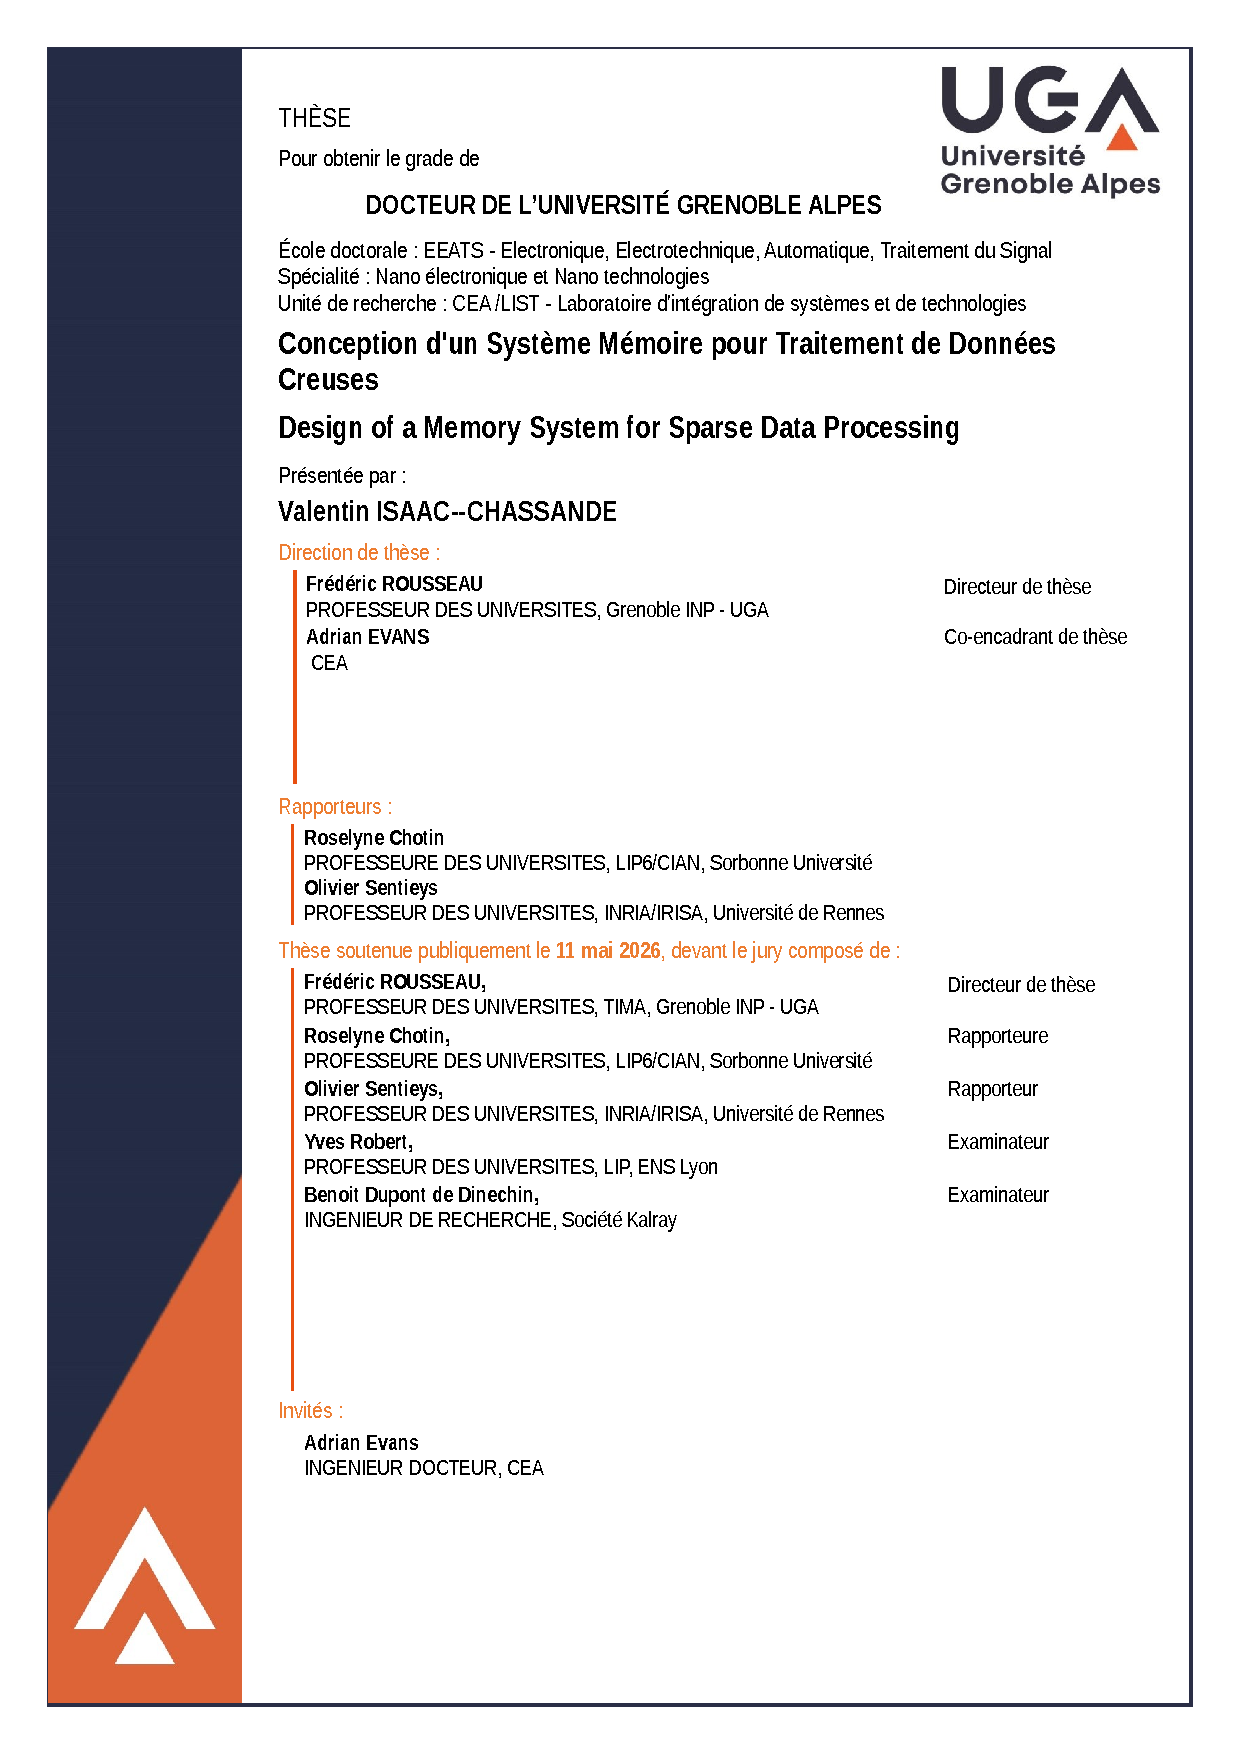
\includepdf[pages=-]{Figures/PDF/couverture_these.pdf}
% %%%%%%%%%%%%%%%%%%%%%%%%%%%%%%%%%%%%%%%%%%%%%%%%%%%%%%%%%%%%%%%%%%%%%

% %%%%%%%%%%%%%%%%%%%%%%%%%%%%%%%%%%%%%%%%%%%%%%%%%%%%%%%%%%%%%%%%%%%%%
% We redefine the title page environment.
% Here is an example of title page:
\begin{titlepage}

%% A A4 PDF to put in the background
% This is just a proposition
% Feel free to modify (you can use the SVGs in Figures/Src as a base)
% See other propositions in Figures/PDF
\ThisULCornerWallPaper{1.0}{Figures/PDF/Fond_Page_de_Garde_CEA-UGA-TIMA}

%% We redefine the page borders. At the end, \restoregeometry is called
%% to go back to the borders defined in Configuration.tex.
\thispagestyle{empty}
\newgeometry{left=1.5cm, right=1.5cm, top=1.50cm, bottom=1.00cm}

\raggedleft
\newlength{\headerheight}
\setlength{\headerheight}{\paperheight-4.5cm}

\begin{minipage}[t][0.2\headerheight]{\linewidth}

    % %% Logos (version with CEA, blanc logos)
    % \raggedleft
    % \newlength{\llogo}
    % \setlength{\llogo}{0.25\linewidth}
    % \begin{minipage}[b][0.5\llogo]{0.12\linewidth}
    %     
\includegraphics[width=\linewidth]{Figures/PDF/LogoBlanc1.pdf}
    %     \vfill
    %     
\includegraphics[width=\linewidth]{Figures/PDF/LogoBlanc2.pdf}
    % \end{minipage}
    % \qquad
    % 
\includegraphics[width=\llogo]{Figures/PDF/LIST.pdf}

    %% Logos (version with CEA, UGA and TIMA)
    \raggedleft
    \newlength{\llogo}
    \setlength{\llogo}{0.25\linewidth}
    \begin{minipage}[b][0.5\llogo]{0.12\linewidth}
        
\includegraphics[width=\linewidth]{Figures/PDF/LogoUGA.pdf}
        \vfill
        
\includegraphics[width=\linewidth]{Figures/PDF/LogoTIMA.pdf}
    \end{minipage}
    \qquad
    
\includegraphics[width=\llogo]{Figures/PDF/LIST.pdf}

    % %% Logos (version with CEA and UGA)
    % \raggedleft
    % \begin{minipage}{0.45\linewidth}
    % 	
\includegraphics[width=0.375\linewidth]{Figures/PDF/LogoUGA.pdf}
    % 	\hfill
    % 	
\includegraphics[width=0.45\linewidth]{Figures/PDF/LIST.pdf}
    % \end{minipage}

\end{minipage}

\centering

\begin{minipage}[t][0.18\headerheight]{\linewidth}
    \normalsize
    \centering

    %% Information about the author. Fill free to add or remove fields
    \textbf{\author}
    	
    Universit\'e Grenoble Alpes
    	
    CEA Grenoble (DRT/LIST/DSCIN/LSTA)
    	
    TIMA Laboratory (SLS)
    
    \textit{ORCID : 0009-0007-9842-5777}
    
    \textit{valentin.isaacchassande@univ-grenoble-alpes.fr}
    
    \textit{valentin.isaacchassande@cea.fr}

\end{minipage}

\begin{minipage}[t][0.08\headerheight]{\linewidth}
    \normalsize
    \centering

    %% The document type defined in Configuration.tex
    \textsc{\doctype}

\end{minipage}

\begin{minipage}[t][0.12\headerheight]{\linewidth}
    \normalsize
    \centering

    %% The title defined in Configuration.tex
    \begin{minipage}{16cm}
        \centering
        \begin{spacing}{2}
    	    \textbf{{\LARGE \textsc{\title}}}
    	\end{spacing}
    \end{minipage}

\end{minipage}

\begin{minipage}[t][0.12\headerheight]{\linewidth}
    \normalsize
    \centering

    %% Date (automatic with that command)
    \today

\end{minipage}

\begin{minipage}[t][0.23\headerheight]{\linewidth}
    \normalsize
    \centering

    %% Some supervisor names (example of a thesis)
    \begin{tabular}{rl}
        Thesis Adviser: & Fr\'ed\'eric ROUSSEAU \\
        Thesis Co-Supervisors: & Adrian EVANS \\
        & Yves DURAND \\
        & \\
        CSI Members: & Yves ROBERT (HDR) \\
        & Christophe PICARD
    \end{tabular}

\end{minipage}

\begin{minipage}[b][0.07\headerheight]{\linewidth}
    \normalsize
    \centering

    %% Any Additional Information
    EEATS Doctoral College, NENT Speciality
    
    \StartYear~-- \EndYear~Academic Years
    
    From \StartDate~to \EndDate

\end{minipage}

\end{titlepage}
% %%%%%%%%%%%%%%%%%%%%%%%%%%%%%%%%%%%%%%%%%%%%%%%%%%%%%%%%%%%%%%%%%%%%%

\restoregeometry
\onehalfspacing %\singlespacing
% %%%%%%%%%%%%%%%%%%%%%%%%%%%%%%%%%%%%%%%%%%%%%%%%%%%%%%%%%%%%%%%%%%%%%%%%%%%%%%%%%%%%%%%
% Acknowledgements
% %%%%%%%%%%%%%%%%%%%%%%%%%%%%%%%%%%%%%%%%%%%%%%%%%%%%%%%%%%%%%%%%%%%%%%%%%%%%%%%%%%%%%%%

\FancyHeadRight{\sectitle}

\if\Language\EN \renewcommand{\sectitle}{Acknowledgements}
\else \renewcommand{\sectitle}{Remerciements} \fi

\phantomsection
\addcontentsline{toc}{chapter}{\sectitle}
\chapter*{\sectitle}

% %%%%%%%%%%%%%%%%%%%%%%%%%%%%%%%%%%%% Your Text %%%%%%%%%%%%%%%%%%%%%%%%%%%%%%%%%%%%%%%%

{\color{red} \textbf{TODO}}

% Fred
% Adrian
% Yves (D)

% Cesar

% Jules

% Yves (R)
% Christophe

% Roselyne
% Olivier

% Benoit
% Yves (R) *
% Fred *

% ---

% LSTA

% Duo Gérôme Ludo

% Alex
% Je remercie Alex, le chef. Bien que je n'ai eu que peu de chef avant lui, il m'a semblé être un chef d'exception, et des dires de gens de plus d'expérience, ce n'est pas qu'une impression !

% Caroline
% Encore une fois, je parle avec peu d'expérience professionnel, et pourtant il me semble évident que Caroline représente la secrétaire modèle, indispensable pour le labo et toujours disponible et entreprenante en plus d'être des plus agréables. Demandez à n'importe qui au LSTA !

% PhD

% Mathieu
% Eduardo
% Davy & Rim
% Joe
% Louis
% Gabriel
% Antoine
% Juan
% Quan
% Junheng
% Yannick

% Joris
% Yann & Meg
% Julien

% Elian
% Mathieu

% Pierre Camille ? ; Yuliana Antoine R Fouad Emma Victor Théo Virgile

% ---

% TIMA
% rester vague trop de monde

% (Chandana)

% Arthur

% ---

% Marin
% Pierre H
% Julien

% Johan (Mathis Cyril Elios)
% Clin d'oeil a ma promo 2022 popo

% ---

% Piano?

% Albert

% Famille

% %%%%%%%%%%%%%%%%%%%%%%%%%%%%%%%%%%%%%%%%%%%%%%%%%%%%%%%%%%%%%%%%%%%%%%%%%%%%%%%%%%%%%%%

\cleardoublepage %% Comment this line if this section occupies the last pages
\adjustmtc
% %%%%%%%%%%%%%%%%%%%%%%%%%%%%%%%%%%%%%%%%%%%%%%%%%%%%%%%%%%%%%%%%%%%%%%%%%%%%%%%%%%%%%%%
% Epigraph
% %%%%%%%%%%%%%%%%%%%%%%%%%%%%%%%%%%%%%%%%%%%%%%%%%%%%%%%%%%%%%%%%%%%%%%%%%%%%%%%%%%%%%%%

\FancyHeadLeft{\sectitle}

\if\Language\EN \renewcommand{\sectitle}{Epigraph}
\else \renewcommand{\sectitle}{Epigraphe} \fi

\phantomsection
\addcontentsline{toc}{chapter}{\sectitle}

\vspace*{7cm}

% %%%%%%%%%%%%%%%%%%%%%%%%%%%%%%%%%%%% Your Text %%%%%%%%%%%%%%%%%%%%%%%%%%%%%%%%%%%%%%%%

\begin{flushright}
    \textit{Quote here. Quote here. Quote here. Quote here. Quote here. Quote here. Quote here. Quote here. Quote here. Quote here.}
    
    \bigskip
    
    Author, "Title".
\end{flushright}

% %%%%%%%%%%%%%%%%%%%%%%%%%%%%%%%%%%%%%%%%%%%%%%%%%%%%%%%%%%%%%%%%%%%%%%%%%%%%%%%%%%%%%%%

\cleardoublepage %% Comment this line if this section occupies the last pages
\adjustmtc
% %%%%%%%%%%%%%%%%%%%%%%%%%%%%%%%%%%%%%%%%%%%%%%%%%%%%%%%%%%%%%%%%%%%%%%%%%%%%%%%%%%%%%%%
% Resume and Abstract
% %%%%%%%%%%%%%%%%%%%%%%%%%%%%%%%%%%%%%%%%%%%%%%%%%%%%%%%%%%%%%%%%%%%%%%%%%%%%%%%%%%%%%%%

\FancyHeadLeft{\sectitle}

\renewcommand{\sectitle}{R\'esum\'e}

\phantomsection
\addcontentsline{toc}{chapter}{\sectitle}
\chapter*{\sectitle}

% %%%%%%%%%%%%%%%%%%%%%%%%%%%%%%%%%%%% Your Text %%%%%%%%%%%%%%%%%%%%%%%%%%%%%%%%%%%%%%%%

{\color{red} \textbf{TODO}}

% %%%%%%%%%%%%%%%%%%%%%%%%%%%%%%%%%%%%%%%%%%%%%%%%%%%%%%%%%%%%%%%%%%%%%%%%%%%%%%%%%%%%%%%

\cleardoublepage %% Comment this line if this section occupies the last pages
\adjustmtc

\if\Language\EN

\FancyHeadLeft{\sectitle}

\renewcommand{\sectitle}{Abstract}

\phantomsection
\addcontentsline{toc}{chapter}{\sectitle}
\chapter*{\sectitle}

% %%%%%%%%%%%%%%%%%%%%%%%%%%%%%%%%%%%% Your Text %%%%%%%%%%%%%%%%%%%%%%%%%%%%%%%%%%%%%%%%

{\color{red} \textbf{TODO}}

% %%%%%%%%%%%%%%%%%%%%%%%%%%%%%%%%%%%%%%%%%%%%%%%%%%%%%%%%%%%%%%%%%%%%%%%%%%%%%%%%%%%%%%%

\cleardoublepage %% Comment this line if this section occupies the last pages
\adjustmtc

\fi
% %%%%%%%%%%%%%%%%%%%%%%%%%%%%%%%%%%%%%%%%%%%%%%%%%%%%%%%%%%%%%%%%%%%%%%%%%%%%%%%%%%%%%%%
% List of Publications
% %%%%%%%%%%%%%%%%%%%%%%%%%%%%%%%%%%%%%%%%%%%%%%%%%%%%%%%%%%%%%%%%%%%%%%%%%%%%%%%%%%%%%%%

\FancyHeadLeft{\sectitle}

\if\Language\EN \renewcommand{\sectitle}{List of Publications}
\else \renewcommand{\sectitle}{Liste des publications} \fi

\phantomsection
\addcontentsline{toc}{chapter}{\sectitle}
\chapter*{\sectitle}

% %%%%%%%%%%%%%%%%%%%%%%%%%%%%%%%%%%%% Your Text %%%%%%%%%%%%%%%%%%%%%%%%%%%%%%%%%%%%%%%%

\noindent This thesis is based on the following publications:
\begin{enumerate}[label=\Roman*, ref=\Roman*, itemsep=0.5cm, topsep=0.5cm]
    %
    \item \label{publ:SoA}
        Valentin Isaac-{-}Chassande, Adrian Evans, Yves Durand, and Frédéric Rousseau. 2024. Dedicated Hardware Accelerators for Processing of Sparse Matrices and Vectors: A Survey. \textit{ACM Trans. Archit. Code Optim.} 21, 2, Article 27 (Feb. 2024), 26 pages.
        Reference~\cite{Isaac2024_SoA}
    %
    \item \label{publ:SpDC}
        Valentin Isaac-{-}Chassande, Adrian Evans, Yves Durand, and Frédéric Rousseau. 2024. SpDCache: Region-Based Reduction Cache for Outer-Product Sparse Matrix Kernels. In \textit{2024 IEEE 35th International Conference on Application-specific Systems, Architectures and Processors (ASAP)}. IEEE Computer Society, Los Alamitos, CA, USA, 3–7.
        Reference~\cite{Isaac2024_SpDCache}
    %
\end{enumerate}

\bigskip \bigskip \bigskip

\noindent The papers will be referred to in the thesis using their Roman numerals.

% %%%%%%%%%%%%%%%%%%%%%%%%%%%%%%%%%%%%%%%%%%%%%%%%%%%%%%%%%%%%%%%%%%%%%%%%%%%%%%%%%%%%%%%

\cleardoublepage %% Comment this line if this section occupies the last pages
\adjustmtc
% %%%%%%%%%%%%%%%%%%%%%%%%%%%%%%%%%%%%%%%%%%%%%%%%%%%%%%%%%%%%%%%%%%%%%%%%%%%%%%%%%%%%%%%
%                             Summary
% %%%%%%%%%%%%%%%%%%%%%%%%%%%%%%%%%%%%%%%%%%%%%%%%%%%%%%%%%%%%%%%%%%%%%%%%%%%%%%%%%%%%%%%

\FancyHeadRight{\sectitle}

\if\Language\EN \renewcommand{\sectitle}{Summary}
\else \renewcommand{\sectitle}{Sommaire} \fi

\phantomsection
\addcontentsline{toc}{chapter}{\sectitle}

\shorttoc{\sectitle}{1}

\cleardoublepage %% Comment this line if this section occupies the last pages
\adjustmtc
% %%%%%%%%%%%%%%%%%%%%%%%%%%%%%%%%%%%%%%%%%%%%%%%%%%%%%%%%%%%%%%%%%%%%%%%%%%%%%%%%%%%%%%%
% Notations
% %%%%%%%%%%%%%%%%%%%%%%%%%%%%%%%%%%%%%%%%%%%%%%%%%%%%%%%%%%%%%%%%%%%%%%%%%%%%%%%%%%%%%%%

\FancyHeadLeft{\sectitle}

\renewcommand{\sectitle}{Notations}

\phantomsection
\addcontentsline{toc}{chapter}{\sectitle}
\chapter*{\sectitle}

% %%%%%%%%%%%%%%%%%%%%%%%%%%%%%%%%%%%% Your Text %%%%%%%%%%%%%%%%%%%%%%%%%%%%%%%%%%%%%%%%

% mathematical notations (double square brackets, etc)
$$\forall (a, b) \in \mathbb{Z}^2, [\![a, b]\!] = [a, b] \cap \mathbb{Z}$$

\bigskip

\begin{center}
    ...
\end{center}

% %%%%%%%%%%%%%%%%%%%%%%%%%%%%%%%%%%%%%%%%%%%%%%%%%%%%%%%%%%%%%%%%%%%%%%%%%%%%%%%%%%%%%%%

\cleardoublepage %% Comment this line if this section occupies the last pages
\adjustmtc
% %%%%%%%%%%%%%%%%%%%%%%%%%%%%%%%%%%%%%%%%%%%%%%%%%%%%%%%%%%%%%%%%%%%%%%%%%%%%%%%%%%%%%%%
% Glossary
% %%%%%%%%%%%%%%%%%%%%%%%%%%%%%%%%%%%%%%%%%%%%%%%%%%%%%%%%%%%%%%%%%%%%%%%%%%%%%%%%%%%%%%%

\FancyHeadRight{\sectitle}

\if\Language\EN \renewcommand{\sectitle}{Glossary}
\else \renewcommand{\sectitle}{Glossaire} \fi

\printnoidxglossary[type=main, sort=letter, title={\sectitle}]

\cleardoublepage %% Comment this line if this section occupies the last pages
\adjustmtc
% %%%%%%%%%%%%%%%%%%%%%%%%%%%%%%%%%%%%%%%%%%%%%%%%%%%%%%%%%%%%%%%%%%%%%%%%%%%%%%%%%%%%%%%
% Acronyms
% %%%%%%%%%%%%%%%%%%%%%%%%%%%%%%%%%%%%%%%%%%%%%%%%%%%%%%%%%%%%%%%%%%%%%%%%%%%%%%%%%%%%%%%

\FancyHeadLeft{\sectitle}

\if\Language\EN \renewcommand{\sectitle}{Acronyms}
\else \renewcommand{\sectitle}{Acronymes} \fi

\printnoidxglossary[type=\acronymtype, title={\sectitle}]

\cleardoublepage %% Comment this line if this section occupies the last pages
\adjustmtc
% %%%%%%%%%%%%%%%%%%%%%%%%%%%%%%%%%%%%%%%%%%%%%%%%%%%%%%%%%%%%%%%%%%%%%%%%%%%%%%%%%%%%%%%
% Introduction
% %%%%%%%%%%%%%%%%%%%%%%%%%%%%%%%%%%%%%%%%%%%%%%%%%%%%%%%%%%%%%%%%%%%%%%%%%%%%%%%%%%%%%%%

\FancyHeadRight{\sectitle}

\renewcommand{\sectitle}{Introduction}

\phantomsection
\chapter*{\sectitle}
\addstarredchapter{\sectitle}

\lettrine{T}{he} rapid growth of data-intensive applications has made sparse and \gls{irrData} structures increasingly prevalent in scientific computing, machine learning, and graph analytics.
However, efficiently processing sparse matrices remains a fundamental challenge due to their inherent irregularity, which leads to unpredictable memory access patterns, limited opportunities for data reuse, and suboptimal utilization of hardware resources.
Existing hardware accelerators have demonstrated various solutions, yet they often rely on restrictive assumptions, exhibit limited scalability, or fail to fully exploit the memory bandwidth.

This thesis addresses the following central question:

\bigskip
\begin{highlight}{Problem Statement}{Mulberry}
    \colorbf{Mulberry}{\emph{How can hardware and architectural mechanisms be designed to efficiently support computation with sparse data, while ensuring scalability, adaptability, and high performance across diverse workloads?}}
\end{highlight}
\bigskip

To tackle this problem, we investigate the limitations of existing algorithms and accelerators, propose a novel cache architecture with support for read-accumulate-write operations, tailored to sparse data.
We then evaluate the behaviour of this specialized cache through modeling, simulation, and hardware prototyping.

\bigskip\bigskip

The manuscript is structured as follows.
We begin with an in-depth discussion of \gls{irrData}, with a particular emphasis on sparse matrices (Chapter~\ref{cha:background}).
This includes a study of fundamental sparse matrix multiplication kernels and their associated algorithms, highlighting the main hardware challenges that arise when dealing with sparse data.
A \gls{highLevel} analysis of algorithms for sparse data computing is provided, with a focus on basic storage schemes and opportunities for data reuse.
Building on this foundation, we review the state-of-the-art in hardware accelerators designed for efficient sparse matrix computing (Chapter~\ref{cha:soa}).
This review identifies common characteristics, proposes a classification of existing accelerators and design tendencies, offers a comparative analysis, and identifies the major tendencies across designs.
This analysis guided our subsequent architectural choices.

Following this survey, we introduce a novel cache architecture specifically designed to address the challenge of read-accumulate-write operations on sparse data, called ``random'' \glspl{reduction} (Chapter~\ref{cha:spdc}).
The proposed cache integrates \gls{reduction} support and organizes its storage into multiple regions optimized for denser and sparser data regions.
A Python model was developed to simulate memory transactions in this cache and to compare its behavior with that of a generic cache.
To further investigate its performance, we complement this analysis with a probabilistic model, that enables rapid simulation and design parameters exploration depending on matrix structure (Chapter~\ref{cha:theory}).

At the micro-architectural level, we detail the virtual partitioning of cache memory into multiple configurable regions, which ensures both flexibility and adaptability to diverse workloads (Chapter~\ref{cha:arch}).
The proposed cache is then evaluated through \acrshort{rtl} simulation, which reveals two distinct classes of matrices that exhibit different performance profiles.
Finally, the manuscript outlines potential future enhancements to improve both performance and scalability, including a multicore extension of the cache architecture and optimizations targeting better usability (Chapter~\ref{cha:optim}).

\section*{Contributions of the Thesis}

The main contributions of this thesis can be summarized as follows:

\begin{enumerate}
    \item \textbf{Analysis of sparse data computing} {\raggedleft \hfill (Chapter~\ref{cha:background})}
    \begin{itemize}
        \item Study of fundamental sparse matrix multiplication kernels and algorithms.
        \item Identification of the hardware challenges associated with sparse data processing.
        \item \Gls{highLevel} analysis of algorithms for sparse data computing, with emphasis on storage schemes and data reuse opportunities.
    \end{itemize}

    \item \textbf{Survey and classification of state-of-the-art accelerators} {\raggedleft \hfill (Chapter~\ref{cha:soa})}
    \begin{itemize}
        \item Comprehensive review of hardware accelerators for sparse matrix computing.
        \item Identification of common architectural features and design tendencies.
        \item Comparative analysis to explain design choices under varying constraints.
    \end{itemize}

    \item \textbf{Design of a cache architecture for ``random'' \glspl{reduction}} {\raggedleft \hfill (Chapter~\ref{cha:spdc})}
    \begin{itemize}
        \item Proposal of a cache with native \gls{reduction} support, capable of handling both dense and sparse data via multiple cache regions.
        \item Development of a Python-based simulation model to analyze memory transactions and benchmark against a generic cache.
    \end{itemize}

    \item \textbf{Probabilistic modeling and exploration of cache behavior} {\raggedleft \hfill (Chapter~\ref{cha:theory})}
    \begin{itemize}
        \item Implementation of a lightweight C-based probabilistic model for rapid simulation.
        \item Exploration of cache dimensioning and behavior across diverse workloads.
    \end{itemize}

    \item \textbf{Micro-architecture and evaluation through \acrshort{rtl} simulation} {\raggedleft \hfill (Chapter~\ref{cha:arch})}
    \begin{itemize}
        \item Introduction of a memory partitioning scheme enabling multiple configurable regions.
        \item Assessment of the proposed cache architecture using \acrshort{rtl}-level simulation.
        \item Identification of two groups of sparse matrices leading to different performance profiles.
    \end{itemize}

    \item \textbf{Future directions for performance and scalability} {\raggedleft \hfill (Chapter~\ref{cha:optim})}
    \begin{itemize}
        \item Extension of the cache architecture to multicore systems for improved scalability.
        \item Optimization techniques to enhance usability and practical deployment.
    \end{itemize}
\end{enumerate}

\cleardoublepage %% Comment this line if this section occupies the last pages
% %%%%%%%%%%%%%%%%%%%%%%%%%%%%%%%%%%%%%%%%%%%%%%%%%%%%%%%%%%%%%%%%%%%%%%%%%%%%%%%%%%%%%%%

% %%%%%%%%%%%%%%%%%%%%%%%%%%%%%%%%%%%%%%%%%%%%%%%%%%%%%%%%%%%%%%%%%%%%%%%%%%%%%%%%%%%%%%%
%                             Header Configuration for Sections
\FancyHeadRight{\leftmark}
% %%%%%%%%%%%%%%%%%%%%%%%%%%%%%%%%%%%%%%%%%%%%%%%%%%%%%%%%%%%%%%%%%%%%%%%%%%%%%%%%%%%%%%%

% %%%%%%%%%%%%%%%%%%%%%%%%%%%%%%%%%%%%%%%%%%%%%%%%%%%%%%%%%%%%%%%%%%%%%%%%%%%%%%%%%%%%%%%
%                             Main Sections
%%%%%%%%%%%%%%%%%%%%%%%%%%%%%%%%%%%%%%%%%%%%%%%%%%%%%%%%%%%%%%%%%%%%%%%%%
% CHAPTER Background
%%%%%%%%%%%%%%%%%%%%%%%%%%%%%%%%%%%%%%%%%%%%%%%%%%%%%%%%%%%%%%%%%%%%%%%%%

\chapter[Background]{Background}
\label{cha:background}

\minitoc

% %%%%%%%%%%%%%%%%%%%%%%%%%%%%%%%%%%%%%%%%%%%%%%%%%%%%%%%%%%%%%%%%%%%%%
% %% Background %%
% Introduction
% %%%%%%%%%%%%%%%%%%%%%%%%%%%%%%%%%%%%%%%%%%%%%%%%%%%%%%%%%%%%%%%%%%%%%

\section{Introduction}
\label{sec:background:intro}

TODO

(Common knowledge on sparse matrices / definitions)

Ref to papers \ref{publ:SoA} and \ref{publ:SpDC} backgrounds.
% %%%%%%%%%%%%%%%%%%%%%%%%%%%%%%%%%%%%%%%%%%%%%%%%%%%%%%%%%%%%%%%%%%%%%
% %% Background %%
% Irregular Accesses
% %%%%%%%%%%%%%%%%%%%%%%%%%%%%%%%%%%%%%%%%%%%%%%%%%%%%%%%%%%%%%%%%%%%%%

\section{Irregular Accesses}
\label{sec:bg:irrAccesses}

TODO
% %%%%%%%%%%%%%%%%%%%%%%%%%%%%%%%%%%%%%%%%%%%%%%%%%%%%%%%%%%%%%%%%%%%%%
% %% Background %%
% Sparse Matrices
% %%%%%%%%%%%%%%%%%%%%%%%%%%%%%%%%%%%%%%%%%%%%%%%%%%%%%%%%%%%%%%%%%%%%%

\section{Sparse Matrices}
\label{sec:bg:spMatrices}

TODO

% sparse matrices / base def (A nnz M N aij ...)

\subsection{Banded Matrices}
\label{sec:bg:bandedMatrices}

TODO
% %%%%%%%%%%%%%%%%%%%%%%%%%%%%%%%%%%%%%%%%%%%%%%%%%%%%%%%%%%%%%%%%%%%%%
% %% Background %%
% Sparse Formats
% %%%%%%%%%%%%%%%%%%%%%%%%%%%%%%%%%%%%%%%%%%%%%%%%%%%%%%%%%%%%%%%%%%%%%

\section{Sparse Formats}
\label{sec:bg:sparse_formats}

\lettrine{I}{n} the absence of a compressed format, matrices are stored in fixed size two-dimensional arrays.
With this \gls{dFormat}, elements can be randomly accessed ($\mathcal{O}(1)$), and \gls{seqAccesses} are highly efficient.
The two dimensions are called \glspl{rank} which correspond to the rows and columns.
For matrices, there are thus two variants of the \gls{dFormat}, depending on which \gls{rank} is stored sequentially in memory.
In a \emph{row-wise} (or \emph{row-major}) storage, the elements within the rows are sequential, and conversely for \emph{column-wise} (or \emph{column-major}). 

Sparse matrices contain a very large number of zeros, and to avoid storing these repeated zeros, there exist many compressed formats~\cite{Tewarson1973_COO_CSR_LIL_first, Kincaid1989_ELLPACK, Barrett1994_CSR_BCSR_DIA_ELL, Saad2003_COO_CSR_DIA_ELL, Bell2009_HYB, Chou2018_COO_CSR_DIA_ELL_HASH}, where certain formats are best-suited for matrices with a specific structure.
The main principle of these \glspl{spFormat} is to avoid storing the zero elements, compensating with additional \gls{metadata} which gives the position of the non-zero elements.

We can cite some of the most used \glspl{spFormat} like \acrfull{coo} that uses three tables of size $nnz$ with only the non-zero elements ($val$ table in Figure~\ref{fig:bg:FormatEx:COO}) and their row and column indices ($row$ and $col$ $idx$ tables).
This format is the simplest one.
It does not need to be sorted to be effective which is a great advantage when the data is ``randomly'' updated.
However, it is an inconvenient for matrix sequential traversals or search tasks.
This format can be sorted \emph{row-wise} as in the example in Figure~\ref{fig:bg:FormatEx:COO} or \emph{column-wise} if needed, but would lose its advantage compared to the two mostly used \glspl{spFormat} \acrfull{csr} (Figure~\ref{fig:bg:FormatEx:CSR}) and its \emph{column-major} counterpart \acrfull{csc} (Figure~\ref{fig:bg:FormatEx:CSC}), which are sorted by construction.
With \acrshort{csc}, the $val$ table of size $nnz$ stores the non-zero elements sorted \emph{column-wise} and the $idx$ table of size $nnz$ stores the corresponding row indices, similarly to \acrshort{coo}.
The third table $ptr$ of size $M+1$ stores the positions of the columns.
For example, in Figure~\ref{fig:bg:FormatEx:CSC}, the second column of index $1$ (\textit{green}) has non-zero elements between positions $2$ and $4$ (\textit{blue}, $4$ excluded) of tables $idx$ and $val$.
This $ptr$ table allows \acrshort{csr} and \acrshort{csc} to have a lower memory footprint than \acrshort{coo}.

\begin{figure}[htbp]
    \centering
    \begin{subfigure}[t]{0.32\linewidth}
        \centering
        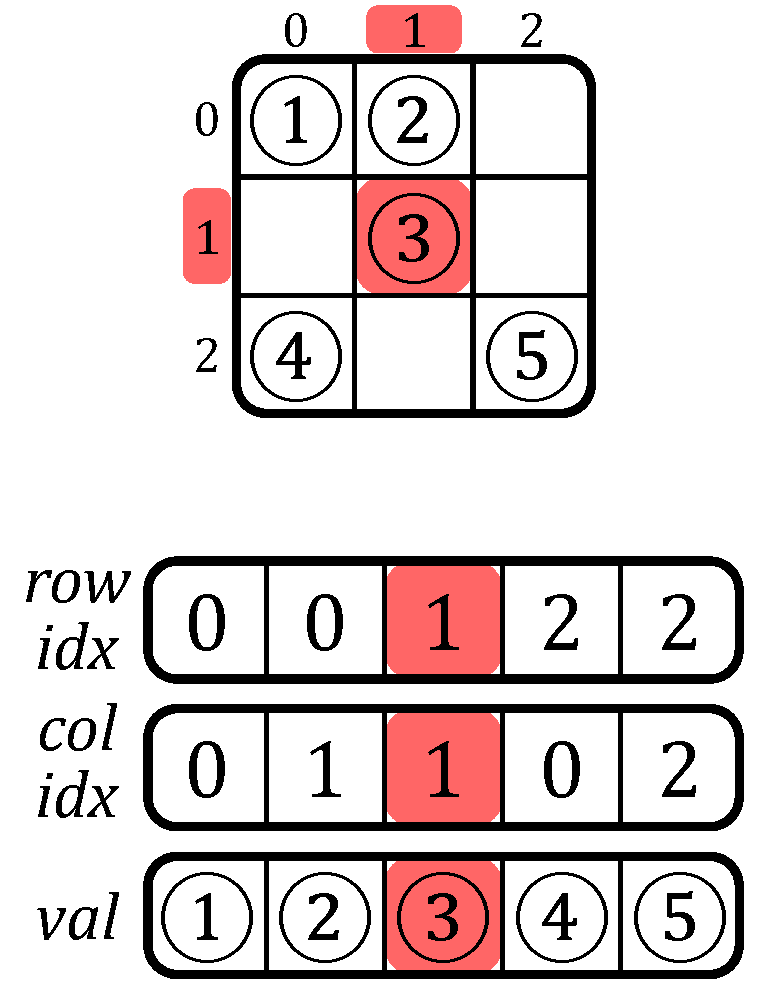
\includegraphics[width=0.8\linewidth]{Chapter_Background/Figures/PDF/SparseFormats/SpFormats_COO.pdf}
        \caption{\acrshort{coo}}
        \label{fig:bg:FormatEx:COO}
    \end{subfigure}
    \hfill
    \begin{subfigure}[t]{0.32\linewidth}
        \centering
        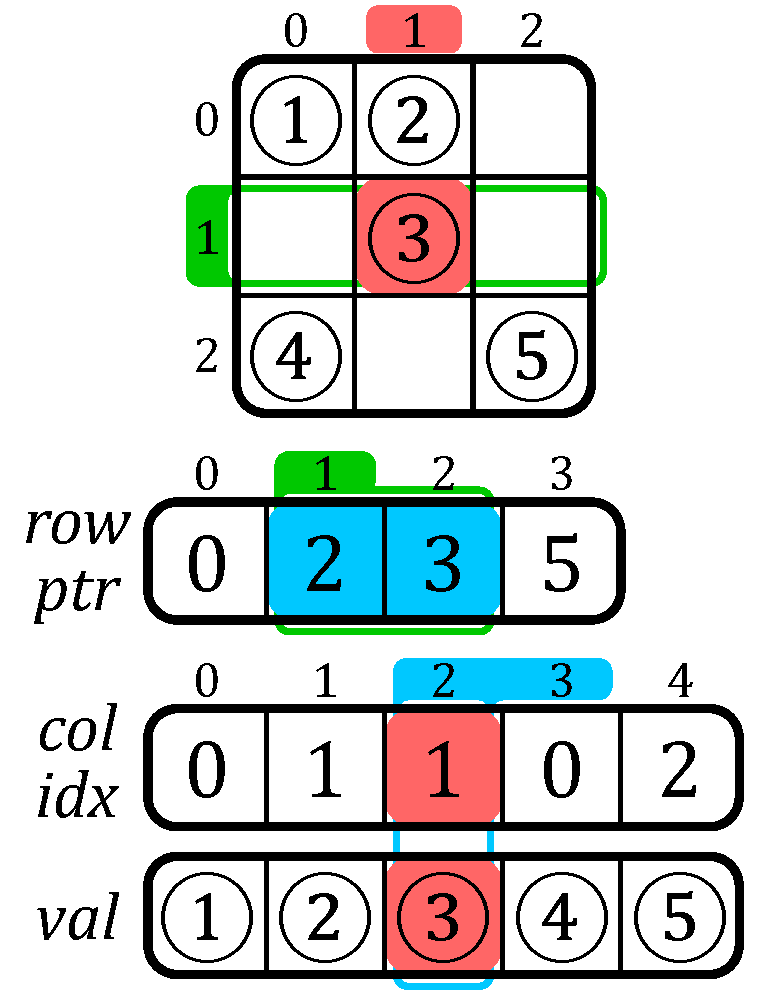
\includegraphics[width=0.8\linewidth]{Chapter_Background/Figures/PDF/SparseFormats/SpFormats_CSR.pdf}
        \caption{\acrshort{csr}}
        \label{fig:bg:FormatEx:CSR}
    \end{subfigure}
    \hfill
    \begin{subfigure}[t]{0.32\linewidth}
        \centering
        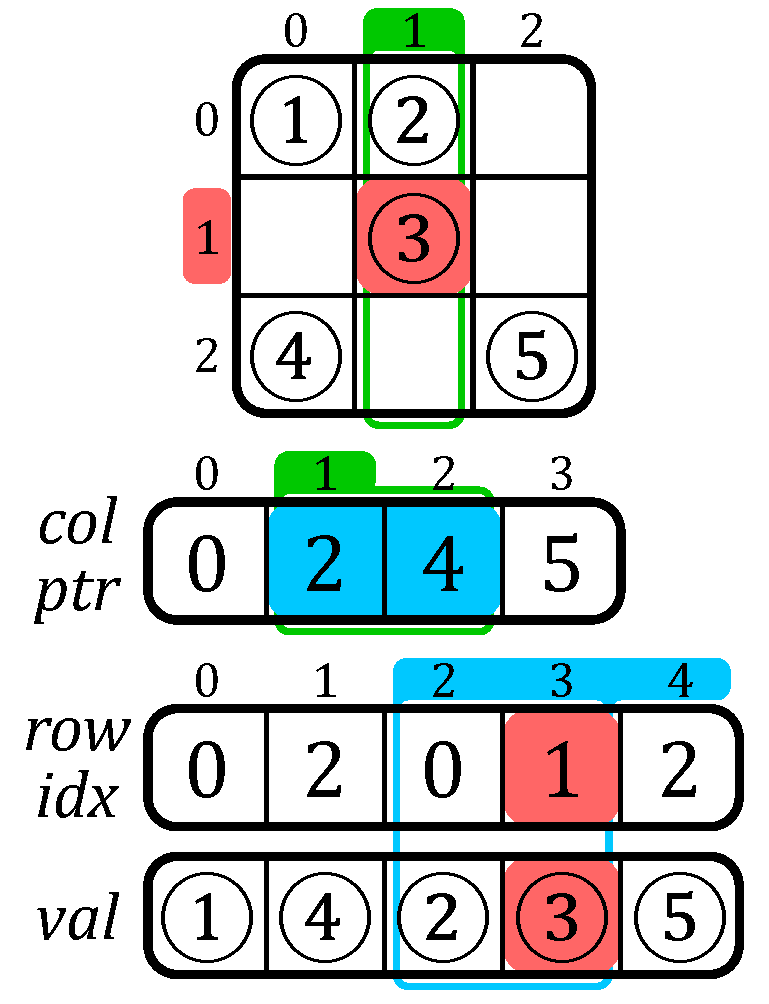
\includegraphics[width=0.8\linewidth]{Chapter_Background/Figures/PDF/SparseFormats/SpFormats_CSC.pdf}
        \caption{\acrshort{csc}}
        \label{fig:bg:FormatEx:CSC}
    \end{subfigure}
    \caption{Example of a Sparse Matrix in \acrshort{coo}, \acrshort{csr} and \acrshort{csc} Formats}
    \label{fig:bg:FormatEx}
\end{figure}

Many others classes of \glspl{spFormat} exists such as \acrfull{bcsr}, \acrfull{dia}, \acrfull{ell} and \acrfull{hyb}, which all have their own advantages depending on the matrix structure or the hardware setup.
Some details on these formats are mentioned in Appendix~\ref{app:sparse_formats}.

In general, there is many derivates from the above main categories of \glspl{spFormat}.
Ultimately, we can create any format we want depending of our needs and constraints in software and hardware.
Latter in this manuscript, we indeed use a custom \gls{spFormat} called \acrfull{bacsc} that is an extension of \acrshort{csc} for \gls{banded} matrices.
As shown in Figure~\ref{fig:bg:FormatEx:BaCSC}, we added extra information in the $ptr$ table to identify the beginning and end of the \gls{band}.
Indeed, three pointers instead of one are now needed per column, as shown with the example of column $2$ in \textit{yellow}.
The column is split in one in-\gls{band} (IB) region in the middle and two out-of-\gls{band} (OB) regions around.
The $ptr$ table size is thus extended to $3 \times M + 1$.
With this format, we can avoid the computational cost of identifying in which region non-zero elements are, while traversing the matrix, a feature we take advantage of in Chapter~\ref{cha:eval}.

\begin{figure}[htbp]
    \centering
    \includegraphics[width=\linewidth]{Chapter_Background/Figures/PDF/SparseFormats/SpFormats_BaCSC.pdf}
    \caption{Example of a Sparse Matrix in \acrshort{bacsc} Format}
    \label{fig:bg:FormatEx:BaCSC}
\end{figure}

\begin{highlight}{Definition}{LimeGreen}
    A \textbf{\gls{spFormat}} is a compression format for sparse matrices, which avoids storing zeros by using \gls{metadata}.
\end{highlight}

\begin{highlight}{Note}{SkyBlue}
    The mostly used \glspl{spFormat} are \acrshort{coo}, \acrshort{csr} and \acrshort{csc}.
\end{highlight}

\begin{highlight}{Conclusion}{Red}
    With the use of \glspl{spFormat}, it is possible to greatly \textbf{decrease memory footprints} while increasing the data dimensions.
    It allows great \textbf{flexibility} to manage data structure in software and hardware.
\end{highlight}
% %%%%%%%%%%%%%%%%%%%%%%%%%%%%%%%%%%%%%%%%%%%%%%%%%%%%%%%%%%%%%%%%%%%%%
% %% Background %%
% Kernels and Algorithms
% %%%%%%%%%%%%%%%%%%%%%%%%%%%%%%%%%%%%%%%%%%%%%%%%%%%%%%%%%%%%%%%%%%%%%

% rank / OP / IP / Gust / tile / tiling / partial outputs / partial sums / intersections

\section{Algorithms for Dense and Sparse Matrix Multiplication}
\label{sec:bg:algos}

The accelerators described in this paper address sparse \acrshort{mv} and \acrshort{mm}.
For \acrshort{mv} we use the notation $A(M,K) \times b(K) = c(M)$ and for \acrshort{mm} the notation $A(M,K) \times B(K,N) = C(M,N)$.
The \emph{rank} $K$ is the \emph{common rank} between the two inputs.

The existence of different \emph{ranks} allows several algorithmic possibilities to compute matrix multiplication: the \acrfull{ip} algorithm, the \acrfull{op} algorithm and \acrlong{gust}'s (\acrshort{gust}) algorithm~\cite{Faddeev1981_InnerOuter, Gustavson1978_GustAlgo}.
In all cases, the matrix $A$ is traversed sequentially.
The three algorithms, however, impose different access patterns for $B$ (or $b$) and $C$ (or $c$).
Indeed, in many cases, they have to be accessed multiple times, as discussed in the following sections.

\subsubsection{Inner-Product Algorithm}

The \acrlong{ip} algorithm~\cite{Faddeev1981_InnerOuter} is an intuitive way to calculate a matrix multiplication because it follows the loop order of the mathematical formulas~(\ref{eq:bg:MVinner}) and~(\ref{eq:bg:MMinner}) for \acrshort{mv} and \acrshort{mm}, respectively.

\begin{equation}
    \forall i \in \ldb0, M-1\rdb, \; c_{i} = \sum_{k = 0}^{K-1} A_{i,k} \times b_{k}
    \label{eq:bg:MVinner}
\end{equation}

\begin{equation}
    \forall (i, j) \in \ldb0, M-1\rdb \times \ldb0, N-1\rdb, \; C_{i, j} = \sum_{k = 0}^{K-1} A_{i,k} \times B_{k,j}
    \label{eq:bg:MMinner}
\end{equation}

The \emph{common rank} $K$ is the inner-most loop of the algorithm (see Algorithms~\ref{alg:bg:MVinner} and~\ref{alg:bg:MMinner}).
The output $C$ (or $c$) is updated sequentially, but the $B$-matrix (or $b$-vector) will be entirely read $M$ times.
In the context of sparse matrices, the reads of $B$ (or $b$) are conditioned by the non-zero elements of $A$, which requires indirect accesses.
If $B$ (or $b$) is also sparse, the algorithm needs to perform \emph{intersections} between the non-zero elements in the rows of $A$ and the columns of $B$ (or in the $b$-vector) (see Section~\ref{sec:bg:hwchallenges}).
In Algorithm~\ref{alg:bg:MMinner}, exchanging $M$ and $N$ simply causes the output to be updated \emph{column-wise}.

\begin{figure}
    \begin{minipage}[t]{0.49\linewidth}
        \begin{algorithm}[H]
        \caption{\acrlong{mv} \acrlong{ip} Algorithm}
        \label{alg:bg:MVinner}
        \For{$i \in \ldb 0, M-1 \rdb$}{
            \For{$k \in \ldb 0, K-1 \rdb$}{
                $c_{i} \acc A_{i,k} \times b_{k}$
            }
        }
        $ $\\
        $ $
        \end{algorithm}
    \end{minipage}
    \hfill
    \begin{minipage}[t]{0.49\linewidth}
        \begin{algorithm}[H]
        \caption{\acrlong{mm} \acrlong{ip} Algorithm}
        \label{alg:bg:MMinner}
        \For{$i \in \ldb 0, M-1 \rdb$}{
            \For{$j \in \ldb 0, N-1 \rdb$}{
                \For{$k \in \ldb 0, K-1 \rdb$}{
                    $C_{i,j} \acc A_{i,k} \times B_{k,j}$
                }
            }
        }
        \end{algorithm}
    \end{minipage}
\end{figure}

\subsubsection{Outer-Product Algorithm}

The \acrlong{op} algorithm~\cite{Faddeev1981_InnerOuter} has the opposite \emph{rank} loop order than the \acrlong{ip}.
It changes nothing mathematically except that the computation is separated into two phases.
First, during the \emph{multiply} phase, we compute several \emph{partial outputs} (\emph{POs}) consisting of the \emph{partial sums} $A_{j,k} \times b_{k}$, then during the \emph{merge} phase, we accumulate all the \emph{POs} to form the final $C$-matrix (or $c$-vector).
Algorithms~\ref{alg:bg:MVouter} and~\ref{alg:bg:MMouter} show that the \emph{common rank} $K$ is the outer-most loop.
Inverting $M$ and $N$ affects whether the output $C$ (or $c$) is updated by rows or by columns, but has no influence on the indirect accesses to the inputs.

\begin{figure}
    \begin{minipage}[t]{0.49\linewidth}
        \begin{algorithm}[H]
        \caption{\acrlong{mv} \acrlong{op} Algorithm}
        \label{alg:bg:MVouter}
        \For{$k \in \ldb 0, K-1 \rdb$}{
            \For{$i \in \ldb 0, M-1 \rdb$}{
                $c_{i} \acc A_{i,k} \times b_{k}$
            }
        }
        $ $\\
        $ $
        \end{algorithm}
    \end{minipage}
    \hfill
    \begin{minipage}[t]{0.49\linewidth}
        \begin{algorithm}[H]
        \caption{\acrlong{mm} \acrlong{op} Algorithm}
        \label{alg:bg:MMouter}
        \For{$k \in \ldb 0, K-1 \rdb$}{
            \For{$i \in \ldb 0, M-1 \rdb$}{
                \For{$j \in \ldb 0, N-1 \rdb$}{
                    $C_{i,j} \acc A_{i,k} \times B_{k,j}$
                }
            }
        }
        \end{algorithm}
    \end{minipage}
\end{figure}

With \acrlong{op}, the $B$-matrix (or $b$-vector) is read sequentially.
This algorithm necessitates the generation of $K$ \emph{POs}.
Moreover, in the context of sparse input matrices, the \emph{PO} element updates are conditioned by the non-zeros elements of both inputs.
Thus, a \emph{partial sum} could potentially be zero, reducing the number of \emph{PO} element updates, and making them non-sequential.
If the output $C$ (or $c$) is stored in a \emph{sparse format}, then it is necessary to repeatedly access and update each \emph{partial sum}.

\subsubsection{Gustavson's Algorithm}

As the \acrshort{mm} algorithm has three \emph{ranks} instead of two for \acrshort{mv}, there is a third ordering, known as \acrlong{gust}'s algorithm~\cite{Gustavson1978_GustAlgo} where the \emph{common rank} $K$ is the middle loop (see Algorithm~\ref{alg:bg:MMgustavson}).
With this approach, the output is computed row-by-row with \emph{PO}-rows generated and accumulated for each output $C$-row.

\begin{figure}
    \centering
    \begin{minipage}[t]{0.49\linewidth}
        \begin{algorithm}[H]
        \caption{\acrlong{mm} \acrlong{gust}'s Algorithm}
        \label{alg:bg:MMgustavson}
        \For{$i \in \ldb 0, M-1 \rdb$}{
            \For{$k \in \ldb 0, K-1 \rdb$}{
                \For{$j \in \ldb 0, N-1 \rdb$}{
                    $C_{i,j} \acc A_{i,k} \times B_{k,j}$
                }
            }
        }
        \end{algorithm}
    \end{minipage}
\end{figure}

With this algorithm, updates of the $C$-rows are sequential, but, in the dense case, the $B$-matrix is entirely read $M$ times and $K$ \emph{PO}-rows of size $N$ are generated.
In the context of sparse matrices, the selection of the rows in $B$ is indirect, however, within a row the accesses are sequential.
The \emph{intersection} operations are only needed for the $B$-rows and not each element.
The \emph{PO}-rows can be accumulated before computing the next $C$-row.
For this algorithm, exchanging $M$ and $N$ causes the three matrices to be accessed \emph{column-wise} instead of \emph{row-wise}.

\subsubsection{Algorithms Comparison}

Note that these algorithms are available in dense as well as in sparse \acrshort{mv} and \acrshort{mm} multiplications.
In sparse, the above algorithms (from \ref{alg:bg:MVinner} to \ref{alg:bg:MMgustavson}) have the same behavior from a software point-of-view, but need adjustments to traverse a \gls{spFormat} instead of a dense matrix.

TODO

\begin{table}
    \centering
    \caption{Comparison of Matrix Multiplication Algorithms}
    \footnotesize
    \begin{tabular}{|>{\centering\arraybackslash}m{1.5cm}|| *{3}{>{\arraybackslash}m{4.2cm}|}}
        \hhline{-||---}
        & \textbf{\acrfull{ip}} & \textbf{\acrfull{op}} & \textbf{\acrfull{gust}} \\
        \hhline{=::===}
        \textbf{A$(M, K)$} \newline \textbf{Accesses} & $\bullet$ read $N$ times\hyperlink{fn3}{$^{\mathrm{1}}$} \newline $\bullet$ \emph{row-wise} \newline $\bullet$ sequential & $\bullet$ read once \newline $\bullet$ \emph{column-wise} \newline $\bullet$ sequential & $\bullet$ read once \newline $\bullet$ \emph{row-wise} \newline $\bullet$ sequential \\
        \hhline{-||---}
        \textbf{B$(K, N)$} \newline \textbf{Accesses} & $\bullet$ read $\overline{nnz_{r}}(A) \times M$ times \newline $\bullet$ \emph{column-wise} \newline $\bullet$ not sequential & $\bullet$ read $\overline{nnz_{c}}(A)$ times\hyperlink{fn4}{$^{\mathrm{2}}$} \newline $\bullet$ \emph{row-wise} \newline $\bullet$ sequential & $\bullet$ read $\overline{nnz_{r}}(A)$ times\hyperlink{fn4}{$^{\mathrm{2}}$} \newline $\bullet$ \emph{row-wise} \newline $\bullet$ sequential within rows \\
        \hhline{-||---}
        \textbf{C$(M, N)$} \newline \textbf{Accesses} & $\bullet$ sequential \newline $\bullet$ generated \emph{row-wise} & $\bullet$ generated without specific structure \newline $\bullet$ $K$ \emph{POs} produced (each \emph{PO} has $nnz_{c}(A) \times nnz_{r}(B)$ non-zero elements) & $\bullet$ generated \emph{row-wise} \newline $\bullet$ for each row, $nnz_{r}(A)$ \emph{PO} rows produced (each \emph{PO} rows has $nnz_{r}(B)$ non-zero elements) \\
        \hhline{-||---}
        \multicolumn{4}{l}{\hypertarget{fn3}{$^{\mathrm{1}}$}In the case of \acrshort{mv} multiplication, $N=1$.} \\
        \multicolumn{4}{l}{\hypertarget{fn4}{$^{\mathrm{2}}$}Average number of non-zero entries in the rows/columns of $A$.}
    \end{tabular}
    \label{tab:AlgosCompSum}
\end{table}

\subsection{Tiling}
\label{sec:bg:tiling}

The \emph{tiling} process~\cite{Grunbaum1987_Tiling} consists in matrix partitioning: a matrix may be divided into \emph{tiles}, non-overlapping sub-matrices.
In other words, this method consists of adding \emph{ranks} to delimit the \emph{tiles}, and thus adding loop iterations in the kernel algorithm.

\emph{Tiling} methods allow to locally reduce the dimensions of data and thus to adapt the working set to the size of the local memory~\cite{Lam1991_Tiling}, particularly when the matrix has a structure with denser regions.
Tiling can also increase parallelism opportunities.
Software optimizations for sparse matrix computation, such as OSKI~\cite{Vuduc2005}, are based on \emph{tiling}.
In previous sections, the study of the \algo{IP}, \algo{OP} and \algo{Gust} algorithms highlighted the influence of \emph{rank} ordering on the sequentiality and data movement, and thus, adding intermediate \emph{ranks} with \emph{tiling} breaks the regularity of pure \algo{IP} or \algo{OP} algorithms, requiring additional hardware support (see Section~\ref{sec:bg:hwchallenges}).

For example, let us consider the $A$-matrix in Figure~\ref{fig:bg:tiling_ex} which is divided into four tiles (one level of \emph{tiling}).
For a SpMV, two new \emph{ranks} appear for a total of four \emph{ranks}: $M_1$ and $K_1$ allow \emph{tile} selection and $M_2$ and $K_2$ allow data access within a \emph{tile}.
Thus, we could decide to apply an \algo{OP} on \emph{tiles} and conversely an \algo{IP} within \emph{tiles}, mixing-up the pros and cons of these two algorithms at different \emph{rank} levels.
In the case of the example in Figure~\ref{fig:bg:tiling_ex}, the upper-left $A$-\emph{tile} (red) is evaluated first, sequentially updating the upper tile of the $c$-vector in an \algo{IP} manner.
The lower-left $A$-\emph{tile} (yellow) is then computed the same way. At this point, \emph{intersections} have been done with only the upper $b$-\emph{tile}, and $c$ has been updated sequentially.
The two next $A$-\emph{tiles} (green, then blue) will compute \emph{intersections} with the lower $b$-\emph{tile} and update the entire $c$-vector sequentially, showing the \algo{OP} characteristic of having \emph{POs} to \emph{merge}, two in this case.
% add ref to algo

\begin{figure}
    \centering
    \begin{minipage}[t]{0.28\linewidth}
        \begin{figure}[H]
            \centering
            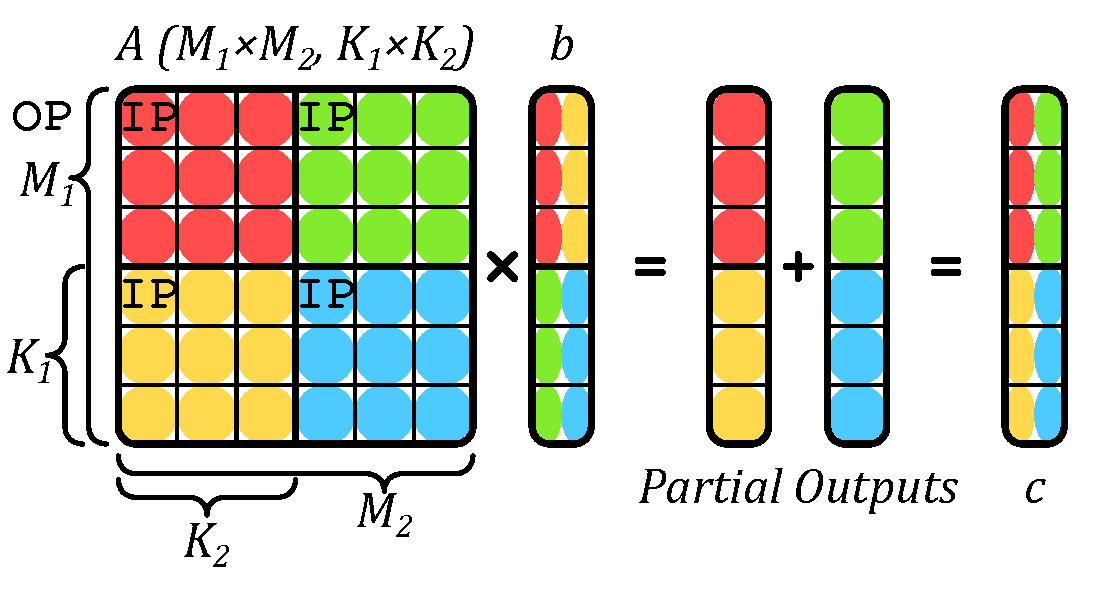
\includegraphics[width=\linewidth]{Chapter_Background/Figures/PDF/TilingExample.pdf}
            \caption{An Example of \Gls{tiling} on \acrshort{spmv}}
            \label{fig:bg:tiling_ex}
        \end{figure}
    \end{minipage}
    \hfill
    \begin{minipage}[t]{0.60\linewidth}
        \bigskip\bigskip
        \begin{algorithm}[H]
        \caption{\acrlong{mv} Algorithm with Custom \Gls{tiling} of Figure~\ref{fig:bg:tiling_ex}}
        \label{alg:bg:tiling_ex}
        \For{$k_1 \in \ldb 0, K_1-1 \rdb$}{
            \For{$i_1 \in \ldb 0, M_1-1 \rdb$}{
                \For{$i_2 \in \ldb 0, M_2-1 \rdb$}{
                    \For{$k_2 \in \ldb 0, K_2-1 \rdb$}{
                        $i \gets i_1 \times M_2 + i_2$\\
                        $k \gets k_1 \times K_2 + k_2$\\
                        $c_i \acc A_{i, k} \times b_k$
                    }
                }
            }
        }
        \end{algorithm}
    \end{minipage}
\end{figure}

Note that in case of \emph{tiling}, the $A$-matrix is no longer read sequentially, which can be problematic if it is stored in a classical \emph{sparse format} like \emph{CSR} that is specifically made for \emph{row-wise} accesses.
Custom \emph{sparse formats} adapted for \emph{tiling} can be used \cite{Im2004_TilingBCSR}, but this requires a preprocessing conversion.
% %%%%%%%%%%%%%%%%%%%%%%%%%%%%%%%%%%%%%%%%%%%%%%%%%%%%%%%%%%%%%%%%%%%%%
% %% Background %%
% Hardware Challenges
% %%%%%%%%%%%%%%%%%%%%%%%%%%%%%%%%%%%%%%%%%%%%%%%%%%%%%%%%%%%%%%%%%%%%%

\section{Hardware Challenges for Sparse Matrix Computation}
\label{sec:bg:hwchallenges}

In the previous section we presented a brief background on matrix multiplication without considering the underlying hardware.
Although the various \emph{sparse formats} reduce the memory footprint, they have the disadvantage that indirect accesses are required, which creates data-dependencies and reduces the effectiveness of caches.
As we have seen, with all three algorithms, at least some of the accesses are non-sequential.
The lack of spatial locality for these accesses reduces the benefit of having caches.
In other words, a full cache line is loaded, but only a few entries are read or modified.
Moreover, the matrices of interest are extremely large and even the non-zero elements, and associated \emph{metadata}, can not generally fit in the cache.
Depending on the algorithm, successive accesses to the same element may be too far apart to benefit from temporal locality in the cache.
% TODO: find the reference

% Perhaps we can add a reference to Yves's background paper where it was stated
% that with typical sparse matrix formats ~50% of the data brought into the
% cache is unused.

%% INNER PRODUCT
In an \algo{IP} algorithm, the $A$-\emph{metadata} needs to be read to indirectly access the $B$-matrix (or $b$-vector), which may itself be stored in a \emph{sparse format}.
In this case, the algorithm needs to check if the non-zero $A$-indices are present in $B$ (or $b$). If an index appears in neither list, there is no need to perform the multiplication (\emph{ineffectual operation}).
More generally, this problem applies to \emph{fibers} and is called the \emph{intersection} search. As a minimum, this requires reading all the \emph{metadata} for $A$ and $B$ (or $b$), and identifying those present in both.

%%%% VL %%%%
In Algorithm~\ref{alg:bg:IPSpMSpMCSR}, we present the pseudo-code for an \emph{inner-product} SpMSpM with $A$ and $B$ stored in \emph{(UOP, CP) row-major} (\emph{CSR}) and \emph{column-major} (\emph{CSC}) formats, respectively.
The outer loop~(\emph{M}), iterates over the rows of $A$, and the first step is to identify the start (\emph{A\_current\_ptr}) and end column (\emph{A\_next\_ptr}) in the \emph{CSR} \emph{metadata}.
The middle-loop (\emph{n}) iterates over the columns of $B$.
The inner-loop iterates over the elements of the current row of $A$, and for each index (\emph{A\_pos}), a search is performed in the \emph{metadata} of $B$, to see if the corresponding index in $B$ is present.
Assuming it is ($B\_pos \neq -1$), the \emph{partial sum} is computed and then accumulated.
This example highlights the need to efficiently search for the intersection of indices in the \emph{metadata} of the inputs.

Different algorithms can be used to address the \emph{intersection} search, depending on whether the elements are sorted.
When the elements are sorted, the \emph{intersection} becomes a merge and generally requires $2 \times k-1$ comparisons (in some cases the number of comparisons can be reduced~\cite{Baeza-Yates2010_Intersection}).
As we will see in Section~\ref{cha:soa}, certain accelerators provide support for performing this intersection operation directly in hardware.

\begin{algorithm}
    \caption{\acrshort{ip} \acrshort{spmspm} Performing \Gls{intersection} Searches with \acrshort{csr} and \acrshort{csc} Formats}
    \label{alg:bg:IPSpMSpMCSR}
    %
    \KwData{$A(M, K)$ in \acrshort{csr}: $\mathit{A.val}, \mathit{A.idx}, \mathit{A.ptr}$}
    \KwData{$B(K, N)$ in \acrshort{csc}: $\mathit{B.val}, \mathit{B.idx}, \mathit{B.ptr}$}
    \KwData{$C(M, N)$ in \gls{dFormat} (for readability)}
    \KwResult{$C = A \times B$}
    \BlankLine
    \For(\tcp*[f]{Iterations over the rows of A}){$i \in \ldb 0, M-1 \rdb$}{
        \For(\tcp*[f]{Iterations over the columns of B}){$j \in \ldb 0, N-1 \rdb$}{
            $acc \gets 0$; $pos_B \gets \mathit{B.ptr}_j$\;
            \For{$pos_A \in \ldb \mathit{A.ptr}_i, \mathit{A.ptr}_{i+1}-1 \rdb$}{
                \tcp{Iterations over the non-zero elements of the i-th row of A}
                $k_A \gets \mathit{A.idx}_{pos_A}$\;
                \tcp{Column-index of the (i, $pos_A$) non-zero element of A}
                $(\mathit{isMatch}, pos_B) \gets \mathit{IntersectionSearch}(k_A, j, pos_B, \mathit{B.idx}, \mathit{B.ptr})$\;
                \tcp{Return true and the matching $pos_B$ if $idx$ exists in the j-th column of B}
                \If(\tcp*[f]{If indices did match}){$\mathit{isMatch}$}{
                    $acc \gets acc + \mathit{A.val}_{pos_A} \times \mathit{B.val}_{pos_B}$\;
                    \tcp{Local partial sum accumulation}
                }
            }
            $C_{i,j} \gets acc$\tcp*[r]{Write in memory of the resulting (i, j) element of C}
        }
    }
    \BlankLine
    \Fn{$\mathit{IntersectionSearch}(k_A, j, pos_B, \mathit{B.idx}, \mathit{B.ptr})$}{
        \tcp{Naive intersection search allowing the i-th row of A and the j-th column of B to be traversed only once at iteration (i, j)}
        \While{$\mathit{B.idx}_{pos_B} < k_A$ \textbf{and} $pos_B < \mathit{B.ptr}_{j+1}$}{
            $pos_B \gets pos_B + 1$\;
        }
        \If(\tcp*[f]{Returns true if indices from A and B match}){$\mathit{B.idx}_{pos_B} = k_A$}{
            \textbf{return} $(true, pos_B)$\;
        }
        \textbf{return} $(false, pos_B)$\;
    }
\end{algorithm}
%%%%%%%%%%%%

%% OUTER PRODUCT
In an \algo{OP} algorithm, the inputs are accessed sequentially, but the updates of the output require indirect accesses.
The pattern of the accesses, while the output is generated, is non-sequential and determined by the structure of the input.
Furthermore, if these \emph{random}\footnote{We use the term \emph{random} to mean accesses are irregular and difficult to predict.} updates provoke cache misses where only one word within a cache-line is modified, the bandwidth to external memory is poorly utilized.
The \algo{OP} algorithm generates several \emph{partial outputs} (\emph{POs}) that must be accumulated to obtain the final output.
We can identify two strategies: \emph{immediate update} and \emph{deferred update}.
In the former, the final output is immediately updated as each \emph{partial sum} is generated.
If the output is stored using a \emph{sparse format}, either the index being updated does not yet exist, and the new \emph{partial sum} must be inserted.
Or, if it exists, a lookup must be done to locate it, the update performed and the result written back.
The problem associated with combining the \emph{POs} is called \emph{reduction}.

%%%% VL %%%%
In Algorithm~\ref{alg:bg:OPSpMSpMCSR}, we present the pseudo-code for an \emph{outer-product} SpMSpM using \emph{immediate update} with A and $B$ stored in \emph{(UOP, CP) column-major} (\emph{CSC}) and \emph{row-major} (\emph{CSR}) formats, respectively.
The outer loop~(\emph{K}), iterates over the rows of A and the columns of $B$ (common rank), and the first step is to identify the start (\emph{A\_current\_ptr, B\_current\_ptr}) and end fibers (\emph{A\_next\_ptr},\emph{B\_next\_ptr}) in the \emph{metadata}.
The middle-loop (\emph{A\_pos}) iterates over the elements of the current column of A.
The inner-loop (\emph{B\_pos}) iterates over the elements of the current row of $B$.
Because we only iterate over the non-zero values, there is no need for a search.
The \emph{partial sum} is then computed. Finally, it must be accumulated to $C_{A\_ind,B\_ind}$.
These accesses are non-sequential, making it necessary to lookup the value in $C$, update it, and write it back, which is performed by the \emph{REDUCTION()} function in the pseudo-code.

% ref for merging methods to add?

\begin{algorithm}
    \caption{\acrshort{op} \acrshort{spmspm} Performing \Gls{reduction} with \acrshort{csr} and \acrshort{csc} Formats}
    \label{alg:bg:OPSpMSpMCSR}
    %
    \KwData{$A(M, K)$ in \acrshort{csr}: $\mathit{A.val}, \mathit{A.idx}, \mathit{A.ptr}$}
    \KwData{$B(K, N)$ in \acrshort{csc}: $\mathit{B.val}, \mathit{B.idx}, \mathit{B.ptr}$}
    \KwData{$\mathit{PO}_k(M, N)$ for all $k \in \ldb 0, K-1 \rdb$ in \acrshort{coo}: $\mathit{PO_k.val}, \mathit{PO_k.row}, \mathit{PO_k.col}$}
    \KwData{$C(M, N)$ in \gls{dFormat} (for readability)}
    \KwResult{$C = A \times B$}
    \BlankLine
    \tcp{* * * `Immediate updates' version * * *}
    \For(\tcp*[f]{Iterations over the columns of A and the rows of $B$}){$k \in \ldb 0, K-1 \rdb$}{
        \For{$pos_A \in \ldb \mathit{A.ptr}_k, \mathit{A.ptr}_{k+1} \rdb$}{
            \tcp{Iterations over the non-zero elements of the k-th column of A}
            $i_A \gets \mathit{A.idx}_{pos_A}$\tcp*[r]{Row-index of the ($pos_A$, k) non-zero element of A}
            \For{$pos_B \in \ldb \mathit{B.ptr}_k, \mathit{B.ptr}_{k+1} \rdb$}{
                \tcp{Iterations over the non-zero elements of the k-th row of B}
                $j_B \gets \mathit{B.idx}_{pos_B}$\;
                \tcp{Column-index of the (k, $pos_B$) non-zero element of B}
                $C_{i_A, j_B} \gets C_{i_A, j_B} + \mathit{A.val}_{pos_A} \times \mathit{B.val}_{pos_B}$\;
                \tcp{Reduction (to memory) of the partial sum into the ($i_A$, $j_B$) element of C (immediate update)}
            }
        }
    }
    \BlankLine
    \tcp{* * * `Deffered updates' version * * *}
    \tcp{Multiply phase}
    \For(\tcp*[f]{Iterations over the columns of A and the rows of $B$}){$k \in \ldb 0, K-1 \rdb$}{
        $pos_\mathit{PO} \gets 0$\;
        \For{$pos_A \in \ldb \mathit{A.ptr}_k, \mathit{A.ptr}_{k+1} \rdb$}{
            \tcp{Iterations over the non-zero elements of the k-th column of A}
            $i_A \gets \mathit{A.idx}_{pos_A}$\tcp*[r]{Row-index of the ($pos_A$, k) non-zero element of A}
            \For{$pos_B \in \ldb \mathit{B.ptr}_k, \mathit{B.ptr}_{k+1} \rdb$}{
                \tcp{Iterations over the non-zero elements of the k-th row of B}
                $j_B \gets \mathit{B.idx}_{pos_B}$\;
                \tcp{Column-index of the (k, $pos_B$) non-zero element of B}
                $\mathit{PO_k.row}_{pos_\mathit{PO}} \gets i_A$\;
                $\mathit{PO_k.col}_{pos_\mathit{PO}} \gets j_B$\;
                $\mathit{PO_k.val}_{pos_\mathit{PO}} \gets \mathit{A.val}_{pos_A} \times \mathit{B.val}_{pos_B}$\; 
                \tcp{The k-th partial sum of the ($i_A$, $j_B$) element of C is stored in memory in the k-th partial output}
                $pos_\mathit{PO} \gets pos_\mathit{PO} + 1$\;
            }
        }
        \tcp{Each partial output is generated sorted, row-wise}
    }
    \tcp{Merge phase}
    \For(\tcp*[f]{Naive serial merge of the K partial outputs}){$k \in \ldb 0, K-2 \rdb$}{
        % $\mathit{MergedPO} \gets \{\}$\;
        % $pos_1 \gets 0$; $pos_2 \gets 0$; $pos_M \gets 0$\;
        % \While{$pos_1 < length(\mathit{PO}_k)$ \textbf{and} $pos_2 < length(\mathit{PO}_{k+1})$}{
        %     \If{$\mathit{PO_k.row}_{pos_1} < \mathit{PO_{k+1}.row}_{pos_2}$}{
        %         $\mathit{MergedPO}_{pos_M} \gets \mathit{PO_k}_{pos_1}$\;
        %         $pos_1 \gets pos_1 + 1$\;
        %     }
        %     \ElseIf{$\mathit{PO_k.row}_{pos_1} > \mathit{PO_{k+1}.row}_{pos_2}$}{
        %         $\mathit{MergedPO}_{pos_M} \gets \mathit{PO_{k+1}}_{pos_2}$\;
        %         $pos_2 \gets pos_2 + 1$\;
        %     }
        %     \Else{
        %         \If{$\mathit{PO_k.col}_{pos_1} < \mathit{PO_{k+1}.col}_{pos_2}$}{
        %             $\mathit{MergedPO}_{pos_M} \gets \mathit{PO_k}_{pos_1}$\;
        %             $pos_1 \gets pos_1 + 1$\;
        %         }
        %         \ElseIf{$\mathit{PO_k.col}_{pos_1} > \mathit{PO_{k+1}.col}_{pos_2}$}{
        %             $\mathit{MergedPO}_{pos_M} \gets \mathit{PO_{k+1}}_{pos_2}$\;
        %             $pos_2 \gets pos_2 + 1$\;
        %         }
        %         \Else{
        %             $\mathit{MergedPO}_{pos_M} \gets \mathit{PO_k}_{pos_1} + \mathit{PO_{k+1}}_{pos_2}$\;
        %             $pos_1 \gets pos_1 + 1$\;
        %             $pos_2 \gets pos_2 + 1$\;
        %         }
        %     }
        %     $pos_M \gets pos_M + 1$\;
        % }
        % \While{$pos_1 < length(\mathit{PO}_k)$}{
        %     $\mathit{MergedPO}_{pos_M} \gets \mathit{PO_k}_{pos_1}$\;
        %     $pos_1 \gets pos_1 + 1$; $pos_M \gets pos_M + 1$\;
        % }
        % \While{$pos_2 < length(\mathit{PO}_{k+1})$}{
        %     $\mathit{MergedPO}_{pos_M} \gets \mathit{PO_{k+1}}_{pos_2}$\;
        %     $pos_2 \gets pos_2 + 1$; $pos_M \gets pos_M + 1$\;
        % }
        $\mathit{PO}_{k+1} \gets \mathit{2DListsMerge}(\mathit{PO}_k, \mathit{PO}_{k+1})$\;
        % $\mathit{PO}_{k+1} \gets \mathit{MergedPO}$\;
    }
    \tcp{$\mathit{PO}_{K-1}$ is C stored in COO format}
    \For{$pos \in \ldb 0, length(\mathit{PO}_{K-1})-1 \rdb$}{
        \tcp{Update C (dense) from the fully merged partial outputs}
        $i \gets \mathit{PO_{K-1}.row}_{pos}$\;
        $j \gets \mathit{PO_{K-1}.col}_{pos}$\;
        $C_{i, j} \gets \mathit{PO_{K-1}.val}_{pos}$\tcp*[r]{Write in memory of the (i, j) element of C}
    }
\end{algorithm}
%%%%%%%%%%%%

% This paragraph covers deferred updates
To avoid the complexities of the indirect accesses with \emph{immediate updates}, the \emph{partial sums} can be stored and the accumulation can be deferred. One such technique is called \emph{output batching}~\cite{Kiriansky2016_Milk}. With this technique, tuples containing the index and the \emph{partial sum} are streamed sequentially to memory. Then, during a second pass, they are read back and the accumulations are performed, an approach which results in sequential memory accesses during the first pass, with the downside that the volume of data transferred to memory is increased.
%%%% VL %%%%
The different strategies for dealing with these updates are shown in Figure~\ref{fig:bg:OutputUpdatesStategies}.
%%%%%%%%%%%%
As we will see, hardware accelerators may combine the \emph{immediate} and \emph{deferred update} techniques to optimize memory bandwidth.
%%%% VL %%%%
\begin{figure}
    \begin{minipage}[b]{0.69\linewidth}
        \begin{figure}[H]% Does it go with a taxonomy in the comparison section?
            \centering
            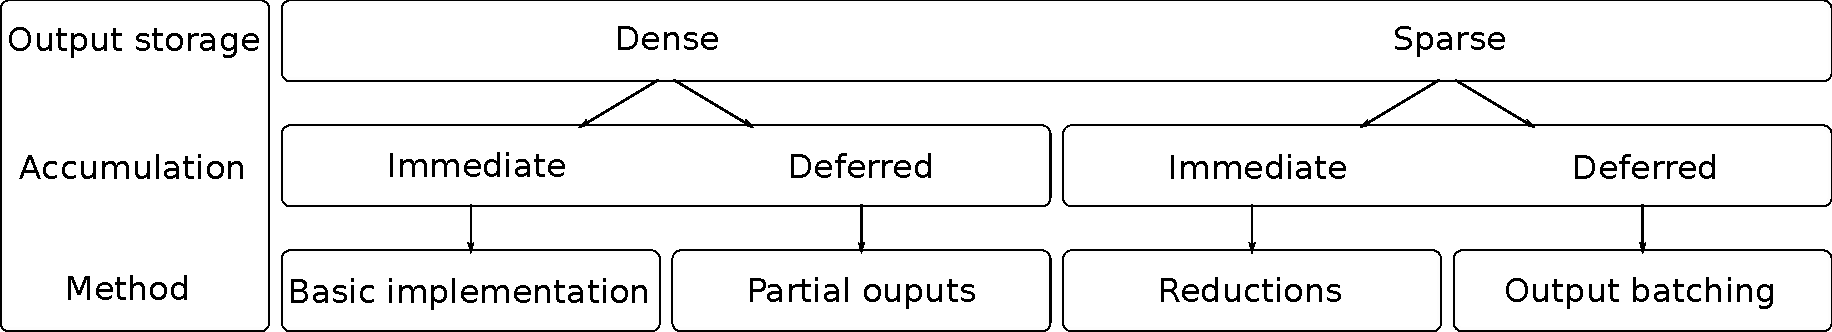
\includegraphics[width=\textwidth]{Chapter_Background/Figures/PDF/OutputUpdates.pdf}
            \caption{Strategies for Dealing with Random Output Updates in Outer Product Algorithms}
            \label{fig:bg:OutputUpdatesStategies}
        \end{figure}
    \end{minipage}
    \hfill
    \begin{minipage}[b]{0.29\linewidth}
        \begin{figure}[H]
            \centering
            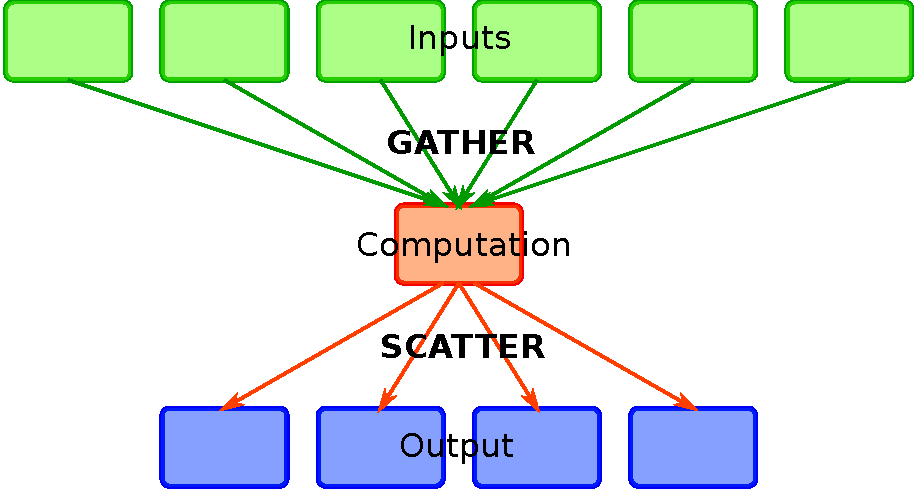
\includegraphics[width=\textwidth]{Chapter_Background/Figures/PDF/GatherScatter.pdf}
            \caption{\emph{Gather} and \emph{Scatter} Illustration}
            \label{fig:bg:gatherscatter}
        \end{figure}
    \end{minipage}
\end{figure}
%%%%%%%%%%%%
In Table~\ref{tab:bg:AlgosHWComp}, we summarize the previously discussed advantages and hardware challenges for each algorithm, including \algo{Gust} which presents a trade-off between \algo{IP} and \algo{OP}.

\begin{table}
    \centering
    \caption{Comparison of Advantages and Challenges with Matrix Multiplication Algorithms}
    \label{tab:bg:AlgosHWComp}
    \begin{tblr}{
            width = {\linewidth},
            colspec = {X[-1,c] X[-1,c] *{3}{X[j]}}, % rowspec
            rows = {m, font=\scriptsize},
            colsep = {4pt},
            row{1-Z} = {rowsep=1pt, black!2},
            row{1} = {c, font=\bfseries\scriptsize, black!5},
            column{1-2} = {font=\bfseries\scriptsize},
            cell{2}{1} = {r=2}{c},
            cell{4-Z}{1} = {c=2}{c},
            cell{5}{3} = {c=2}{l},
            cell{2}{Z} = {c},
            % hlines, vlines,
            % rulesep = {-1pt},
            hline{1,Z} = {2pt}, % Z for last
            hline{2} = {1pt},
            hline{3} = {2-Z}{0.5pt},
            hline{4-Y} = {0.5pt},
            vline{3} = {2-Z}{0.5pt},
        }
        &
        &
        \acrfull{ip} &
        \acrfull{op} &
        \acrfull{gust} \\
        %
        {Access \\ Count} &
        \acrshort{mv} &
        \textbf{\textit{A}:} once ; \textbf{\textit{b}:} $nnz(A)$ ; \textbf{\textit{c}:} once &
        \textbf{\textit{A}:} once ; \textbf{\textit{b}:} once ; \textbf{\textit{c}:} $nnz_{r}(A)$ &
        \emph{N/A} \\
        %
        &
        \acrshort{mm} &
        \textbf{\textit{A}:} $N$ ; \textbf{\textit{B}:} $nnz_{r}(A).M$ ; \newline \textbf{\textit{C}:} once &
        \textbf{\textit{A}:} once ; \textbf{\textit{B}:} $nnz_{c}(A)$ \newline \textbf{\textit{C}:} $\sim nnz_{r}(A).nnz_{c}(B)/K$ &
        \textbf{\textit{A}:} once ; \textbf{\textit{B}:} $nnz_{c}(A)$ \newline \textbf{\textit{C}:} $\sim nnz_{r}(A).nnz_{c}(B)/K$ \\
        %
        {Sequential \\ Accesses} &
        &
        Accesses to $A$ and $C$ &
        Accesses to $A$ and $B$ &
        Accesses to $A$ and $C$ \newline Accesses to $B$-rows \\
        %
        {Input \\ Format} &
        &
        {Accesses to $A$ and $B$ benefit from alternate formats (\emph{CSR} and \\ \emph{CSC})}&
        &
        Allows consistent format for $A$ and $B$ \\
        %
        {Parallelism \\ Opportunity} &
        &
        Possible with \gls{tiling} &
        Generation of \emph{POs} over \emph{common rank} of $A$ and $B$ &
        Reading $A$-rows and updating $C$-rows \\
        %
        {Reuse \\ Opportunity} &
        &
        Potentially $B$, but limited by its size &
        An $A$-column or $B$-row while computing \emph{POs} &
        $A$ set of $B$-rows, based on non-zero elements of $A$-rows \\ %Based on non-zero elements of $A$-rows, a set of $B$-rows are reused
        %
        Challenges &
        &
        \emph{Intersection} search between non-zero elements in $A$ and $B$ &
        Storage for \emph{POs} or in-place  \emph{merge} and \emph{reduce} &
        \emph{Merge} and \emph{reduce} of  \emph{PO rows} \\
    \end{tblr}
\end{table}

% \begin{table}
%     \newlength{\fstC}
%     \setlength{\fstC}{1.00cm}
%     \newlength{\scdC}
%     \setlength{\scdC}{0.65cm}
%     \newlength{\fstAndScdC}
%     \setlength{\fstAndScdC}{2.00cm}
%     \newlength{\lstC}
%     \setlength{\lstC}{4.03cm}
%     \centering
%     \caption{Comparison of Advantages and Challenges with Matrix Multiplication Algorithms}
%     \label{tab:bg:AlgosHWComp}
%     % \footnotesize
%     \scriptsize
%     \begin{tabular}{|>{\arraybackslash\centering}m{\fstC} >{\arraybackslash\centering}m{\scdC}|| *{3}{>{\arraybackslash}m{\lstC}|}}
%         \hhline{--||---}
%         &
%         &
%         \multicolumn{1}{c|}{\textbf{\acrfull{ip}}} &
%         \multicolumn{1}{c|}{\textbf{\acrfull{op}}} &
%         \multicolumn{1}{c|}{\textbf{\acrfull{gust}}} \\
%         %
%         \hhline{==::===}
%         \multirow{3}{\fstC}{\centering\textbf{Access Count}} &
%         \multicolumn{1}{|>{\arraybackslash\centering}m{\scdC}||}{\textbf{MV}} &
%         \textbf{\textit{A}:} once ; \textbf{\textit{b}:} $nnz(A)$ ; \textbf{\textit{c}:} once &
%         \textbf{\textit{A}:} once ; \textbf{\textit{b}:} once ; \textbf{\textit{c}:} $nnz_{r}(A)$ &
%         \multicolumn{1}{c|}{\emph{N/A}} \\
%         %
%         \hhline{~-||---}
%         &
%         \multicolumn{1}{|>{\arraybackslash\centering}m{\scdC}||}{\textbf{MM}} &
%         \textbf{\textit{A}:} $N$ ; \textbf{\textit{B}:} $nnz_{r}(A).M$ ; \newline \textbf{\textit{C}:} once &
%         \textbf{\textit{A}:} once ; \textbf{\textit{B}:} $nnz_{c}(A)$ \newline \textbf{\textit{C}:} $\sim nnz_{r}(A).nnz_{c}(B)/K$ &
%         \textbf{\textit{A}:} once ; \textbf{\textit{B}:} $nnz_{c}(A)$ \newline \textbf{\textit{C}:} $\sim nnz_{r}(A).nnz_{c}(B)/K$ \\
%         %
%         \hhline{--||---}
%         \multicolumn{2}{|>{\arraybackslash\centering}m{\fstAndScdC}||}{\textbf{Sequential Accesses}} &
%         Accesses to $A$ and $C$ &
%         Accesses to $A$ and $B$ &
%         Accesses to $A$ and $C$ \newline Accesses to $B$-rows \\
%         %
%         \hhline{--||---}
%         \multicolumn{2}{|>{\arraybackslash\centering}m{\fstAndScdC}||}{\textbf{Input Format}} &
%         \multicolumn{2}{l|}{\begin{minipage}{7.00cm} Accesses to $A$ and $B$ benefit from alternate formats (\emph{CSR} and \emph{CSC}) \end{minipage}} & 
%         Allows consistent format for $A$ and $B$ \\
%         %
%         \hhline{--||---}
%         \multicolumn{2}{|>{\arraybackslash\centering}m{\fstAndScdC}||}{\textbf{Parallelism Opportunity}} &
%         Possible with \gls{tiling} &
%         Generation of \emph{POs} over \emph{common rank} of $A$ and $B$ &
%         Reading $A$-rows and updating $C$-rows \\
%         %
%         \hhline{--||---}
%         \multicolumn{2}{|>{\arraybackslash\centering}m{\fstAndScdC}||}{\textbf{Reuse Opportunity}} &
%         Potentially $B$, but limited by its size &
%         An $A$-column or $B$-row while computing \emph{POs} &
%         $A$ set of $B$-rows, based on non-zero elements of $A$-rows \\ %Based on non-zero elements of $A$-rows, a set of $B$-rows are reused
%         %
%         \hhline{--||---}
%         \multicolumn{2}{|>{\arraybackslash\centering}m{\fstAndScdC}||}{\textbf{Challenges}} &
%         \emph{Intersection} search between non-zero elements in $A$ and $B$ &
%         Storage for \emph{POs} or in-place  \emph{merge} and \emph{reduce} &
%         \emph{Merge} and \emph{reduce} of  \emph{PO rows} \\
%         %
%         \hhline{--||---}
%     \end{tabular}
% \end{table}

%%%% VC %%%%
The issues presented with \algo{IP} and \algo{OP} can be generalized to two concepts: \emph{gather} and \emph{scatter}.
%%%% VL %%%%
% The issues presented with \emph{inner-product} and \emph{outer-product} can be generalized to two concepts: \emph{gather} and \emph{scatter} (see Figure~\ref{fig:gatherscatter}).
%%%%%%%%%%%%
The \emph{gather} problem exists when the inputs are indirectly accessed, and need to be read from memory using \emph{metadata} to present the processor with the correct terms for computing the \emph{partial sums}. Typically, with \algo{IP}, the \emph{gather} problem is more difficult.
The \emph{scatter} problem exists when the order in which the output matrix/vector is generated is not sequential and is typically associated with the \algo{OP} algorithm.
In the case of \emph{tiling}, a hardware accelerator must handle both \emph{gather} and \emph{scatter}, creating a need for hardware support for both \emph{intersection} searches and \emph{reductions}.

\subsection{SpMSpM Algorithm Analysis}
\label{sec:bg:AnalyticalModel}

To better understand how the algorithms impact the number and types of memory accesses, we developed, and presented in Figure~\ref{fig:bg:AnalyticalModel_SpMSpM}, a model based on memory accesses counts. We identify five memory access patterns: (1) those where a matrix is read only once, thus there is no opportunity for reuse, (2) where the accesses are sequential, but a line is read multiple times, (3) where lines are read consecutively, but the accesses within a line are \emph{random}, (4) where the lines are accessed \emph{randomly}, but within a line the accesses are sequential, and (5) where the matrix elements are accessed multiple times, and with a \emph{random} access pattern.

For each of the three algorithms, we counted the number of read and write accesses, based on the density of the input matrices. We plotted the number of memory accesses in logarithmic scale for SpMSpM, based on a square matrix with $M = 10,000$. Indeed, the number of non-zero elements in $C$ depends on the structure of the input matrices and in this model, we have assumed the non-zero entries in the input matrices are uniformly, randomly distributed. This corresponds to a \emph{worst case} for sparse matrices (no spatial and temporal locality). Banded input matrices would, for example, have fewer non-zero elements in $C$.
In each graph, we have separated the accesses into $A$ (bottom), $B$ (middle) and $C$ (top). The colour code shows the access pattern, based on the five categories described above.

In the top-row of Figure~\ref{fig:bg:AnalyticalModel_SpMSpM} (graphs~\ding{192}, \ding{193} and~\ding{194}), we start by considering a naïve accelerator which has no local storage, thus all data comes from main memory. From these figures, we clearly see that \algo{IP} requires more accesses, as the $A$-matrix must be read N times (graph~\ding{192}). Whereas for \algo{OP} and \algo{Gust}, the $A$-matrix is read only once (thus the grey colour). For \algo{OP} and \algo{Gust} the total number of accesses is the same, however, with \algo{OP} (graph~\ding{193}), the accesses to $C$ are \emph{random} (red). With \algo{Gust} (graph~\ding{194}), the accesses to $B$ are sequential within the rows (orange) and the $C$-rows are generated sequentially (yellow), thus \algo{Gust} avoids having any fully \emph{random} accesses (red).

\begin{figure}
    \centering
    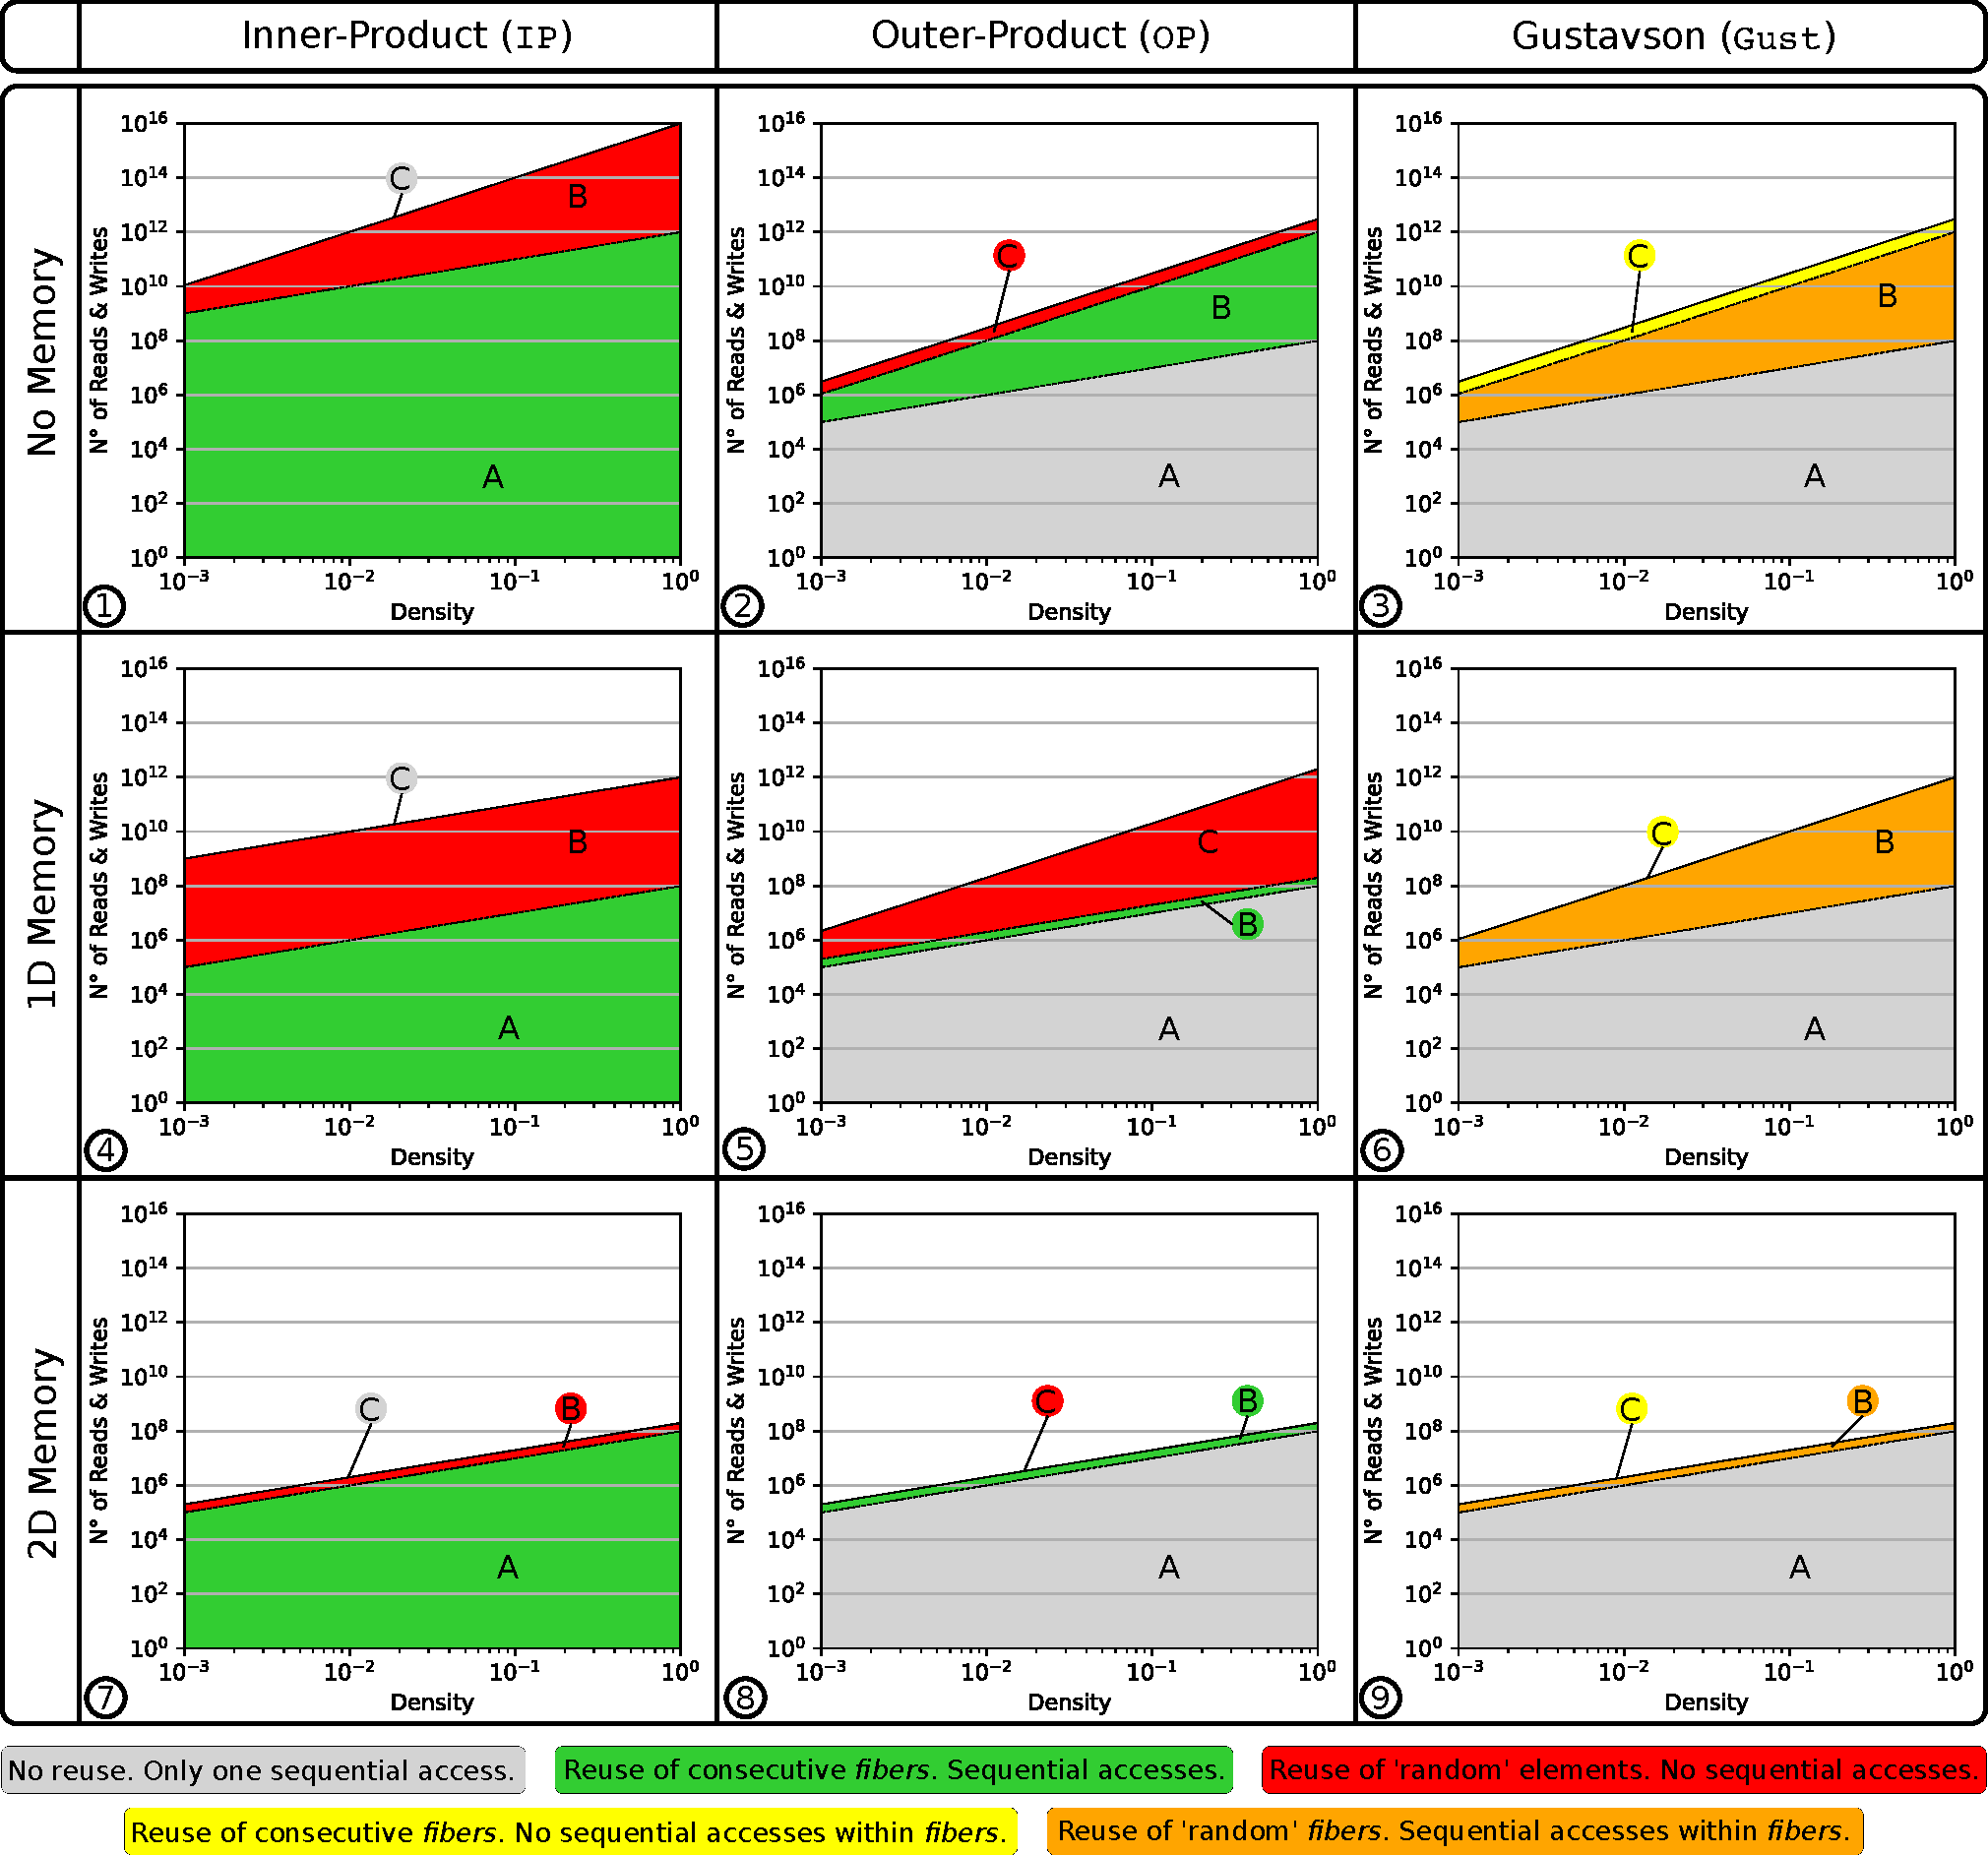
\includegraphics[width=\textwidth]{Chapter_Background/Figures/PDF/AnalyticalModel_SpMSpM.pdf}
    \caption{Model of Memory Access Counts Depending on Algorithm and Local Memory Size}
    \label{fig:bg:AnalyticalModel_SpMSpM}
\end{figure}

Since main memory accesses are the principal bottleneck, accelerators integrate local storage (such as buffers or caches). Thus, we consider the case of an accelerator with sufficient local memory to store one full row, per matrix. We assume this local storage is perfect (no misses) and re-calculate the number of remaining main memory accesses, as shown in the middle-row of Figure~\ref{fig:bg:AnalyticalModel_SpMSpM} (graphs~\ding{195}, \ding{196} and~\ding{197}). The matrices are assumed to be initially stored in main memory, thus they must be accessed at least once.
As can be seen, for \algo{IP} (graph~\ding{195}), the number of $A$-accesses is reduced, because rows are reused, thus the total number of $A$-accesses becomes equal to that in \algo{OP} and \algo{Gust}. For \algo{OP} (graph~\ding{196}), the single row buffer greatly reduces the number of $B$-accesses, however, it does nothing for $C$ (despite the appearance, due to the logarithmic scale). For \algo{Gust} (graph~\ding{197}), the single row buffer is sufficient to cache the \emph{reduction} operations in $C$, and thus, it now has fewer overall accesses than \algo{OP}. It is also interesting to note that \algo{OP} and \algo{Gust} scale better than \algo{IP} with lower densities, as seen by the shallower slope.

Finally, we have considered the extreme case where an accelerator has a buffer of sufficient size to store two matrices, which is shown in the bottom-row of Figure~\ref{fig:bg:AnalyticalModel_SpMSpM} (graphs~\ding{198}, \ding{199} and~\ding{200}). Although this case is not practical for large matrices, through the proper use of \emph{tiling} to locally reduce the dimensions of a sub-matrix, this case can be achieved at the level of a \emph{tile}. In this case, the total number of external accesses is equal for the three algorithms, as each matrix is accessed only once from main memory. For \algo{IP} (graph~\ding{198}), it is interesting to note that such a large buffer is needed to locally address the \emph{intersection} search in $B$. Similarly for \algo{OP} (graph~\ding{199}), a large storage is required to address the \emph{reductions} in $C$. For \algo{Gust}, in fact, it is not necessary to buffer the entire $B$-matrix. Indeed, buffering a few rows (corresponding to $nnz_{r}(A)$) is sufficient to achieve the number of accesses shown in graph~\ding{200}. This corresponds to an intermediate design point (multiple row buffers for $B$) not explicitly shown in the figure (between graphs~\ding{197} and~\ding{200}).

When viewed overall, Figure~\ref{fig:bg:AnalyticalModel_SpMSpM} highlights the benefits of \algo{Gust}. We clearly see that \algo{Gust} does not require any fully \emph{random} accesses (red). With a single row buffer, it is possible to address the \emph{reductions} in $C$. And, with a limited number of row buffers, the number of external memory accesses for $B$ can be reduced. Based on this analysis, it is clear that \algo{Gust} is the best algorithm for hardware implementation of SpMSpM.

% \begin{table}
%     \centering
%     \caption{Caption}
%     \label{tab:my_label}
%     \begin{tabular}{|c|| *{3}{>{\arraybackslash}m{4.15cm}|}}
%         \hhline{-||---}
%          & \textbf{Inner-Product (\algo{IP})} & \textbf{Outer-Product (\algo{OP})} & \textbf{Gustavson (\algo{Gust})} \\
%          \hhline{=::===}
%         \textbf{A$(M,K)$} & 0D: $nnz(A) \times N$ \newline 1D: $nnz(A)$ & 0D: $nnz(A)$ & 0D: $nnz(A)$ \\
%         \hhline{-||---}
%         \textbf{B$(K,N)$} & 0D: $nnz_{r}(A) \times nnz(B) \times M$ \newline $= nnz(A) \times nnz(B)$ \newline 1D: $nnz($B$) \times M$ \newline 2D: $nnz($B$)$ & 0D: $nnz_{c}(A) \times nnz_{r}($B$) \times K$ \newline $= nnz_{c}(A) \times nnz($B$)$ \newline 1D: $nnz_{r}($B$) \times K = nnz($B$)$ & 0D: $nnz_{r}(A) \times nnz_{r}($B$) \times M$ \newline $= nnz(A) \times nnz_{r}($B$)$ \newline 2D: $nnz($B$)$ \\
%         \hhline{-||---}
%         \textbf{C$(M,N)$} & 0D: $nnz(C) \times 2$ \newline (max: $M \times N \times 2$) & 0D: $nnz_{c}(A) \times nnz_{r}($B$) \times K \times 2$ \newline $= nnz_{c}(A) \times nnz($B$) \times 2$ \newline 2D: $nnz(C) \times 2$ \newline (max: $M \times N \times 2$) & 0D: $nnz_{r}(A) \times nnz_{r}($B$) \times M \times 2$ \newline $= nnz(A) \times nnz_{r}($B$) \times 2$ \newline 1D: $nnz(C) \times 2$ \newline (max: $M \times N \times 2$) \\
%         \hhline{-||---}
%     \end{tabular}
% \end{table}
% %%%%%%%%%%%%%%%%%%%%%%%%%%%%%%%%%%%%%%%%%%%%%%%%%%%%%%%%%%%%%%%%%%%%%
% %% Background %%
% Conclusion
% %%%%%%%%%%%%%%%%%%%%%%%%%%%%%%%%%%%%%%%%%%%%%%%%%%%%%%%%%%%%%%%%%%%%%

\section{Conclusion}
\label{sec:bg:conclu}

TODO

\clearpage
%%%%%%%%%%%%%%%%%%%%%%%%%%%%%%%%%%%%%%%%%%%%%%%%%%%%%%%%%%%%%%%%%%%%%%%%%
% CHAPTER State-of-the-Art
%%%%%%%%%%%%%%%%%%%%%%%%%%%%%%%%%%%%%%%%%%%%%%%%%%%%%%%%%%%%%%%%%%%%%%%%%

\chapter[State-of-the-Art]{State-of-the-Art}
\label{cha:soa}

\minitoc

% %%%%%%%%%%%%%%%%%%%%%%%%%%%%%%%%%%%%%%%%%%%%%%%%%%%%%%%%%%%%%%%%%%%%%
% %% State-of-the-Art %%
% Introduction 
% %%%%%%%%%%%%%%%%%%%%%%%%%%%%%%%%%%%%%%%%%%%%%%%%%%%%%%%%%%%%%%%%%%%%%

\section{Introduction}
\label{sec:soa:intro}

TODO

%%%%%%%%%%%%%%%%%

%%drom ASAP intr that can be a short conclu
% The state-of-the-art can be divided into two classes: 
% (1) accelerators that process the entire kernel and (2) accelerators that
% provide a processor assist, typically accelerating either
% the gathering of the inputs or the output scattering.
% Processor assists require less hardware 
% and are more flexible as the main processor executes the kernel.


\note{From SoA paper}

%from intro

It was recognized early in the 1960s~\cite{Saad2003_COO_CSR_DIA_ELL} that working on these sparse data sets using dense array representations was inefficient.
The seminal work of OSKI~\cite{Vuduc2005} in 2003 formalized the sparse representation alternatives and identified many optimizations.
This opened the path for specialized software libraries for sparse algebra~\cite{Williams2007}.
However, the single-core performance of software implementations can be deceiving, often only reaching 10\% of peak performance~\cite{Gale2020}.

%

The two matrix operations, SpMV and SpMSpM, pose orthogonal computational challenges: (1) access to sparse input data, (2) \emph{reduction} operations on the intermediate result and (3) formatting and writing back the result to memory.
The different algorithms, which are detailed in Section~\ref{sec:bg:matrix_formats_and_algos}, are built on different articulations of these three aspects.
% The sparse data storage scheme used in memory dictates the first aspect and is briefly explored in Section~\ref{sec:bg:matrix_formats}.
%The sparse data storage scheme used in memory dictates the first aspect and we explore different alternatives in Subsection~\ref{subsec:matrix_formats}.
The third aspect, \emph{i.e.} result storage, is sometimes overlooked when the output is dense and not too large.
For example, when running on a conventional CPU which is memory-bound, it becomes crucial to streamline the write accesses in order to optimize cache usage when writing a large dense vector output.
The second aspect, \emph{i.e.} the \emph{reduction} operations, deserves different solutions according to the execution platform.
On a conventional CPU, the bottleneck is memory throughput.
Thus, most software implementations of SpMV deal with \emph{a priori} reorganization of the input matrices, by row ordering, blocking and loop optimization, for improving the data locality of operations.
The perspective for SpMV is different when dealing with GPU platforms.
The challenge shifts to finding a balanced assignment of the numerous threads and warps, and to the use of local memory resources~\cite{Liu2014}.
SpMSpM is far more complex: the intermediate \emph{reductions} introduce new $NNZ$ values at random locations, which trigger costly memory allocations and list management operations~\cite{Gao2020}.
As a consequence, this phase dominates the execution time and becomes the main memory bottleneck on a regular CPU.
The issue is similar on GPUs because of the limited size of the scratchpad memory for processing large matrices, which requires complex memory management and load balancing~\cite{Zachariadis2020, Nagasaka2018, Deveci2018}.

%

The main motivation to use custom hardware accelerators is to make better use of the intermediate memory hierarchy, ensuring the input data is available near the cores and also off-loading the accumulation and \emph{reduction} operations from the processors.

The focus of this paper is to review these architectures, to compare them and to analyze their performance. Our main focus is on accelerators that eventually target custom or ASIC implementations, although we do touch on the contributions from accelerators that were prototyped on FPGAs. The reader is referred to~\cite{MOHAMMED_2022_SPARSE} for a survey of acceleration techniques for CPUs, GPUs and FPGAs. Section~\ref{sec:bg:matrix_formats_and_algos} reviews the storage schemes and the three basic algorithms with a focus on the data access patterns and their impact on the memory hierarchy. In Section~\ref{sec:bg:hw_challenges} we study how the different algorithms stress the memory systems and propose an analytical model based on these insights. In Section~\ref{sec:soa:hw_accelerators} we present the operation of several state-of-the-art hardware accelerators, in the light of these hardware challenges. In Section~\ref{sec:soa:comparison_and_analysis}, we systematically compare these accelerators. Throughout this study, we try to be consistent, and we hope that our nomenclature will be useful for architects and designers who intend to implement dedicated hardware for problems with sparse datasets.

% %%%%%%%%%%%%%%%%%%%%%%%%%%%%%%%%%%%%%%%%%%%%%%%%%%%%%%%%%%%%%%%%%%%%%
% Accelerators Section
% %%%%%%%%%%%%%%%%%%%%%%%%%%%%%%%%%%%%%%%%%%%%%%%%%%%%%%%%%%%%%%%%%%%%%

\section{Hardware Accelerators for Sparse Matrices and Vectors}
\label{sec:soa:hw_accelerators}

In this section, we describe the recent (2018-2023) hardware accelerators for sparse MM and MV, targeting ASIC-type implementation. We try to be consistent on notations and architecture schemes to simplify the comparison. Before going into the detailed overviews of the accelerators, in Table~\ref{tab:soa:classificationOverview} we present a criteria-based classification of the designs.

A first criterion to classify the accelerators is between \emph{standalone} accelerators that address the full kernel without the assist of a processor (\emph{e.g.} OuterSPACE~\cite{Pal2018_OuterSPACE} -- Section~\ref{sec:soa:outerspace}) and ones that  address only a part of the kernel and need a processor to manage the computation (\emph{e.g.} PHI~\cite{Mukkara2019_PHI} -- Section~\ref{sec:soa:other_accel}).
\emph{Standalone} accelerators are directly connected to the main memory and internally manage their own custom memories. The other accelerators actually intervene at different levels of the memory hierarchy, giving a second classification criterion. Certain accelerators intervene near the processors (\emph{e.g.} ASA~\cite{Zhang2022_ASA} -- Section~\ref{sec:soa:asa}), near the cache (\emph{e.g.} PHI and SortCache~\cite{Srikanth2021_SortCache} -- Sections~\ref{sec:soa:other_accel} and~\ref{sec:soa:sortcache}), or near the main memory (\emph{e.g.} SPiDRE~\cite{Barredo2019_SPiDRE} and SpaceA~\cite{Xie2021_SpaceA} -- Section~\ref{sec:soa:other_accel}).

Each accelerator is optimized for a specific algorithm (\algo{IP}, \algo{OP} or \algo{Gust}), our third criterion. For example, some accelerators (\emph{e.g.} PHI and SortCache) address the \emph{reduction} problem and are adapted to \algo{OP} algorithms but \emph{reductions} are also required with \algo{Gust} and highly-\emph{tiled} algorithms. ExTensor~\cite{Hegde2019_ExTensor} (Section~\ref{sec:soa:extensor}) is a general purpose accelerator that is demonstrated for a highly-\emph{tiled} \algo{OP} but also makes major contributions for \algo{IP}. 

From a memory perspective, the two main problems are \emph{gather} and \emph{scatter}, our fourth criterion. Certain accelerators offer solutions for one, the other or both. For example, some accelerators (\emph{e.g.} SpArch~\cite{Zhekai2020_SpArch} -- Section~\ref{sec:soa:sparch}) are specialized for an \algo{OP} algorithm but optimize both \emph{gather} and \emph{scatter}. Finally, accelerators preferably focus on sparse MM, MV or both -- our final criterion.

%%%% VL %%%%
% The classification can go further with more details in the different sparse formats used and the data location at each step of a multiplication as presented in Table~\ref{tab:classificationAppView}.

% For each inputs/outputs (including partial outputs), the sparse format used and the place it is stored in memory are described. Moreover, some information is added like the presence of data-rearrangements/hardware conversions for SPiDRE that convert sparse data into a reordered, dense version in main memory and SortCache that use a VBST storage scheme. As some accelerators only address a part of the kernel, the \emph{SW} gray cells indicates whenever the input/output is managed by the software. Thus we naturally find these cells for PHI, SPiDRE, SortCache and ASA. Finally, the \emph{NC} cells are used when the accelerator is not concerned by the partial outputs. This is obviously the case for SPiDRE since it only rearrange data in main memory ahead of time, PHI and SortCache directly generate the final output in caches (there eventually is overflow but we don't consider the resulting intermediate results as partial outputs of the kernel). MatRaptor~\cite{Srivastava2020_MatRaptor}, Gamma and InnerSP~\cite{Baek2021_InnerSP} manage partial output rows to sequentially build the output $C$ with the \emph{Gustavson's} algorithm.

% \begin{table}
%     \caption{Target Applications and Matrix Formats of Existing Accelerators}
%     \begin{center}
%         \footnotesize
%         \begin{tabular}{|c|c| *{4}{| *{2}{>{\centering\arraybackslash}m{1.15cm}|}}}
%             \hhline{--||--------}
%             & \multirow{5}{*}[-0.8ex]{\rotatebox{90}{\begin{minipage}{1.2cm}\raggedright\textbf{Sparse Kernel}\end{minipage}}} & \multicolumn{8}{c|}{\textbf{SpMSpV ($A \times b = c$)} or \textbf{SpMSpM ($A \times B = C$)}} \\
%             & & \multicolumn{8}{c|}{\textit{(NC: not concerned ; SW: managed by the software ; $\xrightarrow{}$: hardware conversion / data-rearrangement ;}} \\
%             & & \multicolumn{8}{c|}{\textit{RA: rearranged format)}} \\
%             \hhline{~~||--------}
%             & & \multicolumn{2}{c||}{\textbf{A}} & \multicolumn{2}{c||}{\textbf{b} or \textbf{B}} & \multicolumn{2}{c||}{\textbf{Partial c} or \textbf{Partial C}} & \multicolumn{2}{c|}{\textbf{c} or \textbf{C}} \\
%             \hhline{~~||--||--||--||--}
%             \textbf{Name} & & \textbf{Format} & \textbf{Stored in} & \textbf{Format} & \textbf{Stored in} & \textbf{Format} & \textbf{Stored in} & \textbf{Format} & \textbf{Stored in} \\
%             \hhline{==::==::==::==::==}
%             OuterSPACE & MM & \emph{(UOP, CP) col.-maj.} & Main memory & \emph{(UOP, CP) row-maj.} & Main memory & \emph{(UOP, CP) col.-maj.} & Main memory & \emph{(UOP, CP) col.-maj.} & Main memory \\
%             \hhline{--||--||--||--||--}
%             ExTensor & MM & \emph{(UOP, CP)}, tiling & Main memory & \emph{(UOP, CP)}, tiling & Main memory & \emph{CP$^{2}$} & Buffer & \emph{CP$^{2}$} & Main memory \\
%             \hhline{--||--||--||--||--}
%             PHI & MV & \multicolumn{2}{c||}{\cellcolor{veryLightGray} SW} & \multicolumn{2}{c||}{\cellcolor{veryLightGray} SW} & \multicolumn{2}{c||}{\cellcolor{lightGray} NC} & \emph{CP} & Caches, Main memory \\
%             \hhline{--||--||--||--||--}
%             SPiDRE & MV & \multicolumn{2}{c||}{\cellcolor{veryLightGray} SW} & \emph{CP $\xrightarrow{}$ RA} & Main memory & \multicolumn{2}{c||}{\cellcolor{lightGray} NC} & \emph{CP $\xrightarrow{}$ RA} & Main memory \\
%             \hhline{--||--||--||--||--}
%             MatRaptor & MM & \emph{(FL, UOP, CP) channel-maj.} & Main memory & \emph{(FL, UOP, CP) channel-maj.} & Main memory & \multicolumn{2}{c||}{\cellcolor{lightGray} NC} & \emph{(UOP, CP) row-maj.} & Main memory \\
%             \hhline{--||--||--||--||--}
%             SpArch & MM & \emph{(UOP, CP) row-maj.}, condensed column & Main memory & \emph{(UOP, CP) row-maj.} & Main memory & \emph{CP$^{2}$ row-maj.} & Main memory & \emph{(UOP, CP) row-maj.} & Main memory \\
%             \hhline{--||--||--||--||--}
%             Gamma & MM & \emph{(UOP, CP) row-maj.} & Main memory & \emph{(UOP, CP) row-maj.} & Internal cache & \multicolumn{2}{c||}{\cellcolor{lightGray} NC} & \emph{(UOP, CP) row-maj.} & Main memory \\
%             \hhline{--||--||--||--||--}
%             InnerSP & MM & \emph{(UOP, CP) row-maj.} & Main memory & \emph{(UOP, CP) row-maj.} & Main memory & \multicolumn{2}{c||}{\cellcolor{lightGray} NC} & \emph{(UOP, CP) row-maj.} & Main memory \\
%             \hhline{--||--||--||--||--}
%             SortCache & MM & \multicolumn{2}{c||}{\cellcolor{veryLightGray} SW} & \multicolumn{2}{c||}{\cellcolor{veryLightGray} SW} & \multicolumn{2}{c||}{\cellcolor{lightGray} NC} & \emph{(UOP, CP) $\xrightarrow{}$ VBST} & Caches \\
%             \hhline{--||--||--||--||--}
%             ASA & MM & \multicolumn{2}{c||}{\cellcolor{veryLightGray} SW} & \multicolumn{2}{c||}{\cellcolor{veryLightGray} SW} & \emph{CP} & Internal cache, Main memory & \emph{(UOP, CP)} &SPiDRE Main memory \\
%             \hhline{--||--||--||--||--}
%             GSCSp & MM & \emph{(UOP, CP) row-maj.} & Main memory & \emph{(UOP, CP) row-maj.} & Internal cache & \multicolumn{2}{c||}{\cellcolor{lightGray} NC} & \emph{(UOP, CP) row-maj.} & Main memory \\
%             \hhline{--||--||--||--||--}
%         \end{tabular}
%         \label{tab:classificationAppView}
%     \end{center}
% \end{table}
%%%%%%%%%%%%

After this first comparison, in Sections~\ref{sec:soa:outerspace} to~\ref{sec:soa:gamma} we present the \emph{standalone} accelerators, followed by the \emph{processor assist} accelerators in Sections~\ref{sec:soa:sortcache} to~\ref{sec:soa:asa}. In Section~\ref{sec:soa:other_accel}, we briefly touch on other accelerators.

% \begin{table}
%     \caption{Algorithmic and Architectural Classification of Existing Accelerators}
%     \begin{center}
%         \footnotesize
%         \begin{tabular}{|c|| *{2}{>{\centering\arraybackslash}p{0.5cm}|}| *{3}{>{\centering\arraybackslash}p{0.5cm}|}| *{3}{>{\centering\arraybackslash}p{0.5cm}|}| *{2}{>{\centering\arraybackslash}p{0.5cm}|} |c|}
%             \hhline{-||--||---||---||--||-}
%             & \multicolumn{2}{c||}{} & \multicolumn{3}{c||}{\textbf{Position in}} & \multicolumn{3}{c||}{\textbf{Most Adapted}} & \multicolumn{2}{c||}{\textbf{Hardware}} & \\
%             & \multicolumn{2}{c||}{\textbf{Autonomy}} & \multicolumn{3}{c||}{\textbf{Memory Hierarchy}} & \multicolumn{3}{c||}{\textbf{Algorithm}} & \multicolumn{2}{c||}{\textbf{Support for}} & \multirow{2}{*}[9.3ex]{\rotatebox{90}{\begin{minipage}{2.6cm}\raggedright\textbf{Sparse Kernels Addressed}\end{minipage}}} \\
%             \hhline{~||--||---||---||--||~}
%             \textbf{Name} & \rotatebox{90}{\textbf{\textit{Standalone}}} & \rotatebox{90}{\begin{minipage}{1.34cm}\raggedright\textbf{\textit{Processor Assist}}\end{minipage}} & \rotatebox{90}{\begin{minipage}{1.3cm}\raggedright\textbf{\textit{Near Processors}}\end{minipage}} & \rotatebox{90}{\begin{minipage}{1.3cm}\raggedright\textbf{\textit{Near Cache}}\end{minipage}} & \rotatebox{90}{\begin{minipage}{1.3cm}\raggedright\textbf{\textit{Near Main Memory}}\end{minipage}} & \rotatebox{90}{\begin{minipage}{1.3cm}\raggedright\textbf{\textit{Inner-product}}\end{minipage}} & \rotatebox{90}{\begin{minipage}{1.3cm}\raggedright\textbf{\textit{Outer-product}}\end{minipage}} & \rotatebox{90}{\textbf{\textit{Gustavson}}} & \rotatebox{90}{\textbf{\textit{Gather}}} & \rotatebox{90}{\textbf{\textit{Scatter}}} &  \\
%             \hhline{=::==::===::===::==::=}
%             OuterSPACE~\cite{Pal2018_OuterSPACE} & \cellcolor{darkGray} & & \multicolumn{3}{c||}{\textit{N/A}} & & \cellcolor{darkGray} & & \cellcolor{darkGray} & \cellcolor{darkGray} & MV, MM \\
%             \hhline{-||--||---||---||--||-}
%             ExTensor~\cite{Hegde2019_ExTensor} & \cellcolor{darkGray} & & \multicolumn{3}{c||}{\textit{N/A}} & \cellcolor{darkGray} & \cellcolor{veryLightGray} \hspace{1.0em} \hyperlink{fn5}{$^{\mathrm{a}}$} & & \cellcolor{darkGray} & \cellcolor{veryLightGray} \hspace{1.0em} \hyperlink{fn5}{$^{\mathrm{a}}$} & MV\hyperlink{fn6}{$^{\mathrm{b}}$}, MM \\
%             \hhline{-||--||---||---||--||-}
%             PHI~\cite{Mukkara2019_PHI} & & \cellcolor{darkGray} & & \cellcolor{darkGray} & & & \cellcolor{darkGray} & \cellcolor{veryLightGray} \hspace{1.0em} \hyperlink{fn6}{$^{\mathrm{b}}$} & & \cellcolor{darkGray} & MV, MM\hyperlink{fn6}{$^{\mathrm{b}}$} \\
%             \hhline{-||--||---||---||--||-}
%             SPiDRE~\cite{Barredo2019_SPiDRE} & & \cellcolor{darkGray} & & & \cellcolor{darkGray} & \cellcolor{darkGray} & & & \cellcolor{darkGray} & & MV, MM\hyperlink{fn6}{$^{\mathrm{b}}$} \\
%             \hhline{-||--||---||---||--||-}
%             MatRaptor~\cite{Srivastava2020_MatRaptor} & \cellcolor{darkGray} & & \multicolumn{3}{c||}{\textit{N/A}} & & & \cellcolor{darkGray} & \cellcolor{darkGray} & \cellcolor{darkGray} & MM \\
%             \hhline{-||--||---||---||--||-}
%             SpArch~\cite{Zhekai2020_SpArch} & \cellcolor{darkGray} & & \multicolumn{3}{c||}{\textit{N/A}} & & \cellcolor{darkGray} & & \cellcolor{darkGray} & \cellcolor{darkGray} & MM \\
%             \hhline{-||--||---||---||--||-}
%             Gamma~\cite{Zhang2021_Gamma} & \cellcolor{darkGray} & & \multicolumn{3}{c||}{\textit{N/A}} & & & \cellcolor{darkGray} & \cellcolor{darkGray} & \cellcolor{veryLightGray} \hspace{1.0em} \hyperlink{fn5}{$^{\mathrm{a}}$} & MM \\
%             \hhline{-||--||---||---||--||-}
%             InnerSP~\cite{Baek2021_InnerSP} & \cellcolor{darkGray} & & \multicolumn{3}{c||}{\textit{N/A}} & & & \cellcolor{darkGray} & \cellcolor{darkGray} & \cellcolor{darkGray} & MM \\
%             \hhline{-||--||---||---||--||-}
%             SortCache~\cite{Srikanth2021_SortCache} & & \cellcolor{darkGray} & & \cellcolor{darkGray} & & & \cellcolor{darkGray} & \cellcolor{veryLightGray} \hspace{1.0em} \hyperlink{fn6}{$^{\mathrm{b}}$} & & \cellcolor{darkGray} & MV\hyperlink{fn6}{$^{\mathrm{b}}$}, MM \\
%             \hhline{-||--||---||---||--||-}
%             ASA~\cite{Zhang2022_ASA} & & \cellcolor{darkGray} & \cellcolor{darkGray} & & & & \cellcolor{veryLightGray} \hspace{1.0em} \hyperlink{fn6}{$^{\mathrm{b}}$} & \cellcolor{darkGray} & & \cellcolor{darkGray} & MV\hyperlink{fn6}{$^{\mathrm{b}}$}, MM \\
%             \hhline{-||--||---||---||--||-}
%             Flexagon~\cite{Munoz-Martinez2023_Flexagon} & \cellcolor{darkGray} & & \multicolumn{3}{c||}{\textit{N/A}} & \cellcolor{darkGray} & \cellcolor{darkGray} & \cellcolor{darkGray} & \cellcolor{darkGray} & \cellcolor{darkGray} & MM \\
%             \hhline{-||--||---||---||--||-}
%             GSCSp~\cite{LI_2023_GSCSp} & \cellcolor{darkGray} & & \multicolumn{3}{c||}{\textit{N/A}} & & & \cellcolor{darkGray} & \cellcolor{darkGray} & \cellcolor{darkGray} & MM \\
%             \hhline{-||--||---||---||--||-}
%             \multicolumn{6}{l}{Gray cell: the accelerator meets the criterion.} & \multicolumn{6}{r}{\hypertarget{fn5}{$^{\mathrm{a}}$}Not main contribution but addressed in the article.} \\
%             \multicolumn{12}{r}{\hypertarget{fn6}{$^{\mathrm{b}}$}Could be adapted but not discussed in the article.}
%         \end{tabular}
%         \label{tab:classificationOverview}
%     \end{center}
% \end{table}

\begin{table}
    \caption{Algorithmic and Architectural Classification of Existing Accelerators}
    \begin{center}
        \footnotesize
        \begin{tabular}{|c|c|| *{2}{>{\centering\arraybackslash}p{0.5cm}|}| *{3}{>{\centering\arraybackslash}p{0.5cm}|}| *{3}{>{\centering\arraybackslash}p{0.5cm}|}| *{2}{>{\centering\arraybackslash}p{0.5cm}|} |c|}
            \hhline{--||--||---||---||--||-}
            & & \multicolumn{2}{c||}{} & \multicolumn{3}{c||}{\textbf{Position in}} & \multicolumn{3}{c||}{\textbf{Most Adapted}} & \multicolumn{2}{c||}{\textbf{Hardware}} & \\
            & & \multicolumn{2}{c||}{\textbf{Autonomy}} & \multicolumn{3}{c||}{\textbf{Memory Hierarchy}} & \multicolumn{3}{c||}{\textbf{Algorithm}} & \multicolumn{2}{c||}{\textbf{Support for}} & \multirow{2}{*}[9.3ex]{\rotatebox{90}{\begin{minipage}{2.6cm}\raggedright\textbf{Sparse Kernels Addressed}\end{minipage}}} \\
            \hhline{~~||--||---||---||--||~}
            \textbf{Name} & \textbf{Date} & \rotatebox{90}{\textbf{\textit{Standalone}}} & \rotatebox{90}{\begin{minipage}{1.34cm}\raggedright\textbf{\textit{Processor Assist}}\end{minipage}} & \rotatebox{90}{\begin{minipage}{1.3cm}\raggedright\textbf{\textit{Near Processors}}\end{minipage}} & \rotatebox{90}{\begin{minipage}{1.3cm}\raggedright\textbf{\textit{Near Cache}}\end{minipage}} & \rotatebox{90}{\begin{minipage}{1.3cm}\raggedright\textbf{\textit{Near Main Memory}}\end{minipage}} & \rotatebox{90}{\begin{minipage}{1.3cm}\raggedright\textbf{\textit{Inner-product}}\end{minipage}} & \rotatebox{90}{\begin{minipage}{1.3cm}\raggedright\textbf{\textit{Outer-product}}\end{minipage}} & \rotatebox{90}{\textbf{\textit{Gustavson}}} & \rotatebox{90}{\textbf{\textit{Gather}}} & \rotatebox{90}{\textbf{\textit{Scatter}}} &  \\
            \hhline{==::==::===::===::==::=}
            OuterSPACE~\cite{Pal2018_OuterSPACE} & 2018 & \cellcolor{darkGray} & & \multicolumn{3}{c||}{\textit{N/A}} & & \cellcolor{darkGray} & & \cellcolor{darkGray} & \cellcolor{darkGray} & MV, MM \\
            \hhline{--||--||---||---||--||-}
            ExTensor~\cite{Hegde2019_ExTensor} & 2019 & \cellcolor{darkGray} & & \multicolumn{3}{c||}{\textit{N/A}} & \cellcolor{darkGray} & \cellcolor{veryLightGray} \hspace{1.0em} \hyperlink{fn5}{$^{\mathrm{a}}$} & & \cellcolor{darkGray} & \cellcolor{veryLightGray} \hspace{1.0em} \hyperlink{fn5}{$^{\mathrm{a}}$} & MV\hyperlink{fn6}{$^{\mathrm{b}}$}, MM \\
            \hhline{--||--||---||---||--||-}
            PHI~\cite{Mukkara2019_PHI} & 2019 & & \cellcolor{darkGray} & & \cellcolor{darkGray} & & & \cellcolor{darkGray} & \cellcolor{veryLightGray} \hspace{1.0em} \hyperlink{fn6}{$^{\mathrm{b}}$} & & \cellcolor{darkGray} & MV, MM\hyperlink{fn6}{$^{\mathrm{b}}$} \\
            \hhline{--||--||---||---||--||-}
            SPiDRE~\cite{Barredo2019_SPiDRE} & 2019 & & \cellcolor{darkGray} & & & \cellcolor{darkGray} & \cellcolor{darkGray} & & & \cellcolor{darkGray} & & MV, MM\hyperlink{fn6}{$^{\mathrm{b}}$} \\
            \hhline{--||--||---||---||--||-}
            MatRaptor~\cite{Srivastava2020_MatRaptor} & 2020 & \cellcolor{darkGray} & & \multicolumn{3}{c||}{\textit{N/A}} & & & \cellcolor{darkGray} & \cellcolor{darkGray} & \cellcolor{darkGray} & MM \\
            \hhline{--||--||---||---||--||-}
            SpArch~\cite{Zhekai2020_SpArch} & 2020 & \cellcolor{darkGray} & & \multicolumn{3}{c||}{\textit{N/A}} & & \cellcolor{darkGray} & & \cellcolor{darkGray} & \cellcolor{darkGray} & MM \\
            \hhline{--||--||---||---||--||-}
            SpaceA~\cite{Xie2021_SpaceA} & 2021 & \cellcolor{darkGray} & & & & \cellcolor{darkGray} & \cellcolor{darkGray} & & & \cellcolor{darkGray} & \cellcolor{darkGray} & MV \\
            \hhline{--||--||---||---||--||-}
            Gamma~\cite{Zhang2021_Gamma} & 2021 & \cellcolor{darkGray} & & \multicolumn{3}{c||}{\textit{N/A}} & & & \cellcolor{darkGray} & \cellcolor{darkGray} & \cellcolor{veryLightGray} \hspace{1.0em} \hyperlink{fn5}{$^{\mathrm{a}}$} & MM \\
            \hhline{--||--||---||---||--||-}
            InnerSP~\cite{Baek2021_InnerSP} & 2021 & \cellcolor{darkGray} & & \multicolumn{3}{c||}{\textit{N/A}} & & & \cellcolor{darkGray} & \cellcolor{darkGray} & \cellcolor{darkGray} & MM \\
            \hhline{--||--||---||---||--||-}
            SortCache~\cite{Srikanth2021_SortCache} & 2021 & & \cellcolor{darkGray} & & \cellcolor{darkGray} & & & \cellcolor{darkGray} & \cellcolor{veryLightGray} \hspace{1.0em} \hyperlink{fn6}{$^{\mathrm{b}}$} & & \cellcolor{darkGray} & MV\hyperlink{fn6}{$^{\mathrm{b}}$}, MM \\
            \hhline{--||--||---||---||--||-}
            ASA~\cite{Zhang2022_ASA} & 2022 & & \cellcolor{darkGray} & \cellcolor{darkGray} & & & & \cellcolor{veryLightGray} \hspace{1.0em} \hyperlink{fn6}{$^{\mathrm{b}}$} & \cellcolor{darkGray} & & \cellcolor{darkGray} & MV\hyperlink{fn6}{$^{\mathrm{b}}$}, MM \\
            \hhline{--||--||---||---||--||-}
            Flexagon~\cite{Munoz-Martinez2023_Flexagon} & 2023 & \cellcolor{darkGray} & & \multicolumn{3}{c||}{\textit{N/A}} & \cellcolor{darkGray} & \cellcolor{darkGray} & \cellcolor{darkGray} & \cellcolor{darkGray} & \cellcolor{darkGray} & MM \\
            \hhline{--||--||---||---||--||-}
            GSCSp~\cite{LI_2023_GSCSp} & 2023 & \cellcolor{darkGray} & & \multicolumn{3}{c||}{\textit{N/A}} & & & \cellcolor{darkGray} & \cellcolor{darkGray} & \cellcolor{darkGray} & MM \\
            \hhline{--||--||---||---||--||-}
            \multicolumn{7}{l}{Gray cell: the accelerator meets the criterion.} & \multicolumn{6}{r}{\hypertarget{fn5}{$^{\mathrm{a}}$}Not main contribution but addressed in the article.} \\
            \multicolumn{13}{r}{\hypertarget{fn6}{$^{\mathrm{b}}$}Could be adapted but not discussed in the article.}
        \end{tabular}
        \label{tab:soa:classificationOverview}
    \end{center}
\end{table}

%%%%%%%%%%%%%%%%%%%%%%%%%%%%%%%%%%%%%%%%%%%%%%%%%%%%%%%%%%%%%%%%%%%%%%%%%%%%%%%%%%%%%%%%%%%%%%%%%%%%%%%%%%%%
% Complete accelerators

% %%%%%%%%%%%%%%%%%%%%%%%%%%%%%%%%%%%%%%%%%%%%%%%%%%%%%%%%%%%%%%%%%%%%%
% %% State-of-the-Art %%
% OuterSPACE
% %%%%%%%%%%%%%%%%%%%%%%%%%%%%%%%%%%%%%%%%%%%%%%%%%%%%%%%%%%%%%%%%%%%%%

\subsection{OuterSPACE}
\label{sec:soa:outerspace}

OuterSPACE~\cite{Pal2018_OuterSPACE} is an \algo{OP} accelerator with a focus on SpMSpM kernels, although it can also handle SpMV. It is a highly parallelized architecture which employs Single-Program Multiple-Data (SPMD)-style \emph{processing elements} (\emph{PEs}) that fetch data from main memory through a two-level highly-banked cache hierarchy as shown in Figure~\ref{fig:soa:outerspace}. The input $A$- and $B$-matrices are stored in \emph{(UOP, CP) column-} and \emph{row-major} formats, respectively, to match the read access patterns of the \algo{OP} algorithm. The \emph{partial} and final outputs are stored in \emph{(UOP, CP)} format.

The computation is temporally divided into the \emph{multiply} and \emph{merge} phases (Figure~\ref{fig:soa:outerspaceHow}). During the first phase, inputs are divided into \emph{tiles} of several rows~($A$) and columns~($B$) and distributed through the \emph{processing tiles} (\emph{PTs}) by a \emph{control unit}. Within each \emph{PT}, each \emph{PE} processes multiplications of one element of the $k^{th}$ $A$-column with all elements of the $k^{th}$ $B$-row and an L0 cache in the \emph{PT} facilitates the reuse of the $B$-rows between \emph{PEs}. This phase generates a \emph{partial output} (\emph{PO}) per \emph{PT}, corresponding to the \emph{tile} of rows~($A$) and columns~($B$) that it was assigned.

Then, during the \emph{merge} phase, the \emph{POs} are combined to generate the final $C$-matrix. Each \emph{PT} locally sorts the \emph{POs}, and then the \emph{PTs} work together to merge them. This algorithm was chosen to maximize data locality and parallelism, although it is less efficient. This \emph{merge} phase only uses half of the \emph{PEs} so the others are disabled (clock-gated) and the caches are reconfigured in a scratchpad mode to save energy.

Note, if $NNZ$ elements in the \emph{POs} exceeds the L0 cache capacity, it overflows to the last level cache, which results in reduced performance. OuterSPACE performs best when the $NNZ_c(A)$ and $NNZ_r(B)$ are both uniform which ensures a uniform distribution of work across the large number of \emph{PTs} and \emph{PEs}.

\begin{figure}
    \centering
    \begin{minipage}[b]{0.49\linewidth}
        \begin{figure}[H]
            \centering
            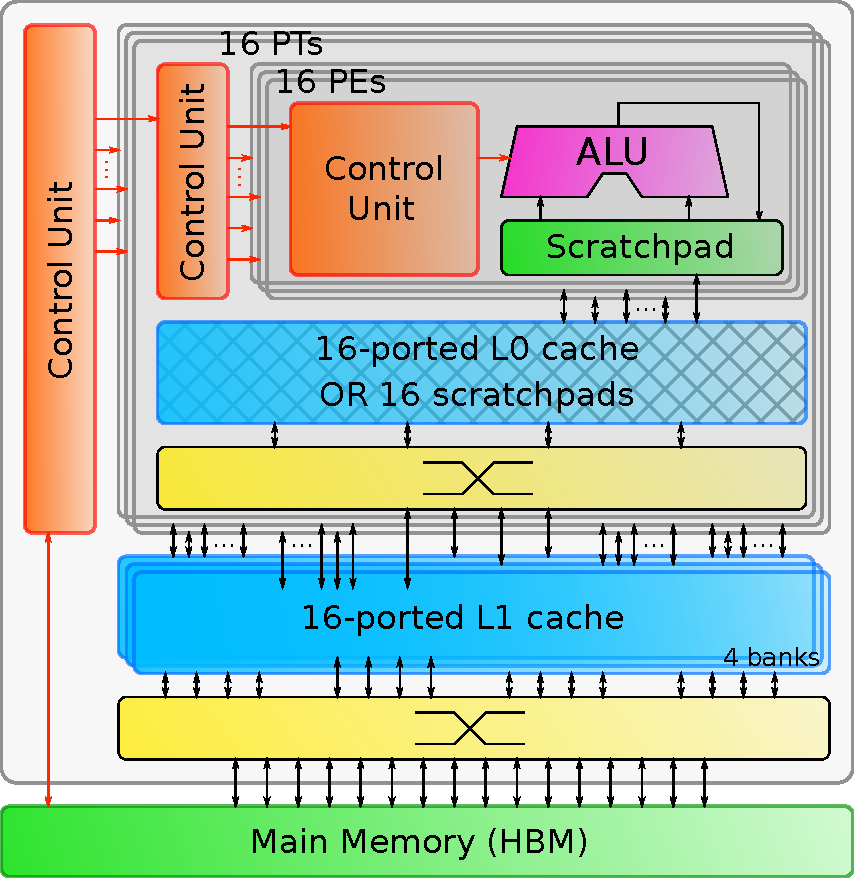
\includegraphics[width=0.7\textwidth]{Chapter_SoA/Figures/PDF/OuterSPACE.pdf}
            \caption{Architecture of OuterSPACE}
            \label{fig:soa:outerspace}
        \end{figure}
    \end{minipage}
    \hfill
    \begin{minipage}[b]{0.49\linewidth}
        \begin{figure}[H]
            \centering
            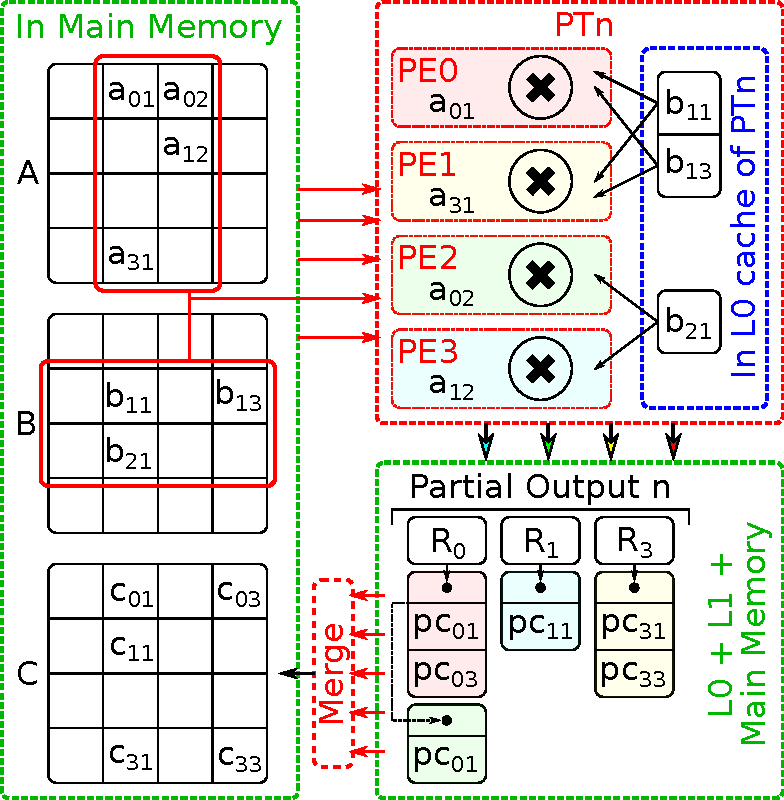
\includegraphics[width=0.705\textwidth]{Chapter_SoA/Figures/PDF/OuterSPACE_How_Vertical.pdf}
            \caption{OuterSPACE Data Flow}
            \label{fig:soa:outerspaceHow}
        \end{figure}
    \end{minipage}
\end{figure}

% %%%%%%%%%%%%%%%%%%%%%%%%%%%%%%%%%%%%%%%%%%%%%%%%%%%%%%%%%%%%%%%%%%%%%
% %% State-of-the-Art %%
% ExTensor
% %%%%%%%%%%%%%%%%%%%%%%%%%%%%%%%%%%%%%%%%%%%%%%%%%%%%%%%%%%%%%%%%%%%%%

\subsection{ExTensor}
\label{sec:soa:extensor}

The authors created ExTensor~\cite{Hegde2019_ExTensor} as a general purpose sparse tensor algebra accelerator (including SpMSpM). It is an \algo{OP} accelerator but due to its support for three levels of fixed \emph{tiling} of the inputs, it optimizes the \emph{intersection} search between non-zero elements or \emph{tiles}\footnote{Tensauraus~\cite{Srivastava2020_Tensaurus} is another accelerator designed for tensors, but their focus is on SpMM.}. By doing the \emph{intersections} ahead of time, at different levels of the memory hierarchy (which correspond to the \emph{tile} levels), ExTensor is able to efficiently eliminate \emph{ineffectual operations}, thus addressing the main issue in \algo{IP} or complex \emph{tiling} algorithms. Indeed, the input matrices would typically be stored in an \emph{(UOP, UOP, UOP, CP}) format, corresponding to three levels of \emph{tiling}.
ExTensor is designed with a flexible architecture composed of different bricks (see Figure~\ref{fig:soa:extensor}). To simply aid in the understanding, the interactions between the bricks are described using function calls:
\begin{itemize}
    \item The \emph{Scanner} is a storage unit that delivers a stream of coordinates in increasing order, fetching them from memory. The coordinates are delivered through the \emph{Iterate()} operation call.
    \item The \emph{Intersect} is a hardware block that co-iterates over several \emph{Scanners} in parallel and compares the coordinate streams. This unit performs the \emph{intersection} search required by \algo{IP} type algorithms, delivering a single stream with the matching coordinates, which are the coordinates of non-zero \emph{partial sums}. To optimise the \emph{intersection} step, it is possible to skip a range of coordinates in a stream depending on the current coordinate of another stream. Thus, the \emph{Intersect} sends skip messages with \emph{SkipTo()} operations to the other \emph{Scanners}.
    \item The \emph{Coordinator} is a hardware unit that includes \emph{Scanners} and \emph{Intersect} units, and manages the input and output data depending on the current processed \emph{tile}, as shown in Figure~\ref{fig:soa:extensor}. Data and \emph{metadata} are respectively stored in storage units and \emph{Scanners}, while a \emph{Sequencer} manages the \emph{Iterate()} calls so that the \emph{Intersect} brick delivers the stream of effective coordinates. In addition, in the \emph{Tile Coord} brick, the offsets of the \emph{tile} are added back, so the output of the \emph{Coordinator} is in absolute coordinates.
\end{itemize}

These bricks can be placed at different positions in a memory hierarchy, depending on the \emph{tiling} and selected hardware. Thus, the \emph{Coordinator} is able to intersect at coarse-granularity with output data being \emph{metadata} of the next \emph{tile}, skipping an entire \emph{tile} when appropriate, with low computation cost, and also at fine-granularity when output data are the non-zero elements that need to be multiplied.

ExTensor is designed with three levels of \emph{tiling} that each have  either input or output sequentiality. First, a \emph{Sequencer} plus \emph{Scanners} block~\ding{192} is placed close to the main memory to determine which \emph{tiles} to send to the next storage, the \emph{Last Level Buffer} (\emph{LLB}). Then, for each \emph{tile}, a \emph{Coordinator}~\ding{193} in the \emph{LLB} intersects the next level \emph{tiles}, which are sent to several \emph{PEs} that will process in parallel. Finally, in each \emph{PE}, a \emph{Coordinator}~\ding{194} intersects the non-zero elements of the computed \emph{tile} and sends them to the arithmetic unit of the \emph{PE} for multiplication.

In addition to these bricks which are the main contributions, ExTensor still needs to perform the \emph{merge} phase, including the \emph{reduction} of the \emph{POs} which are stored in \emph{CP$^{2}$} format. The \emph{Partial Output Buffer} (\emph{POB}), is managed by \emph{tiles}, and the content of the \emph{tile} is stored on-chip using a Content Addressable Memory (CAM) for quick access, enabling \emph{reductions} to be performed. On overflow, the \emph{tiles} are flushed to main memory. To benefit from ExTensor's support for \emph{tiling}, the input matrices need preprocessing, making it difficult to directly compare performance with other accelerators.

\begin{figure}
    \centering
    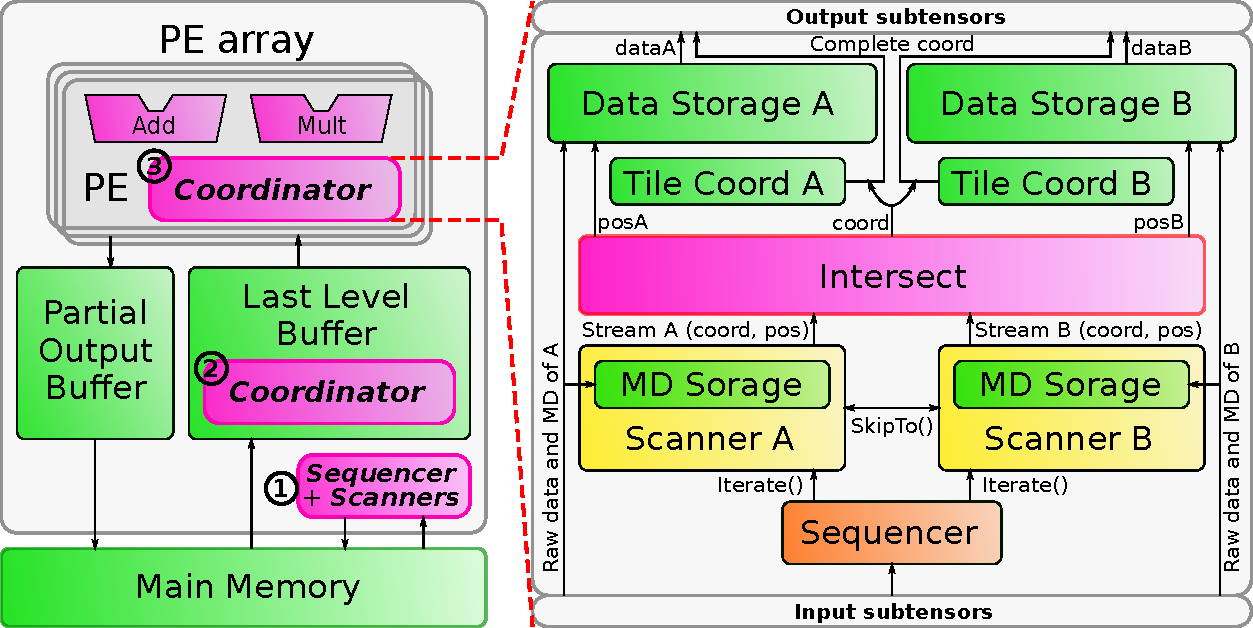
\includegraphics[width=0.6\linewidth]{Chapter_SoA/Figures/PDF/ExTensor.pdf}
    \caption{Architecture of ExTensor}
    \label{fig:soa:extensor}
\end{figure}

% %%%%%%%%%%%%%%%%%%%%%%%%%%%%%%%%%%%%%%%%%%%%%%%%%%%%%%%%%%%%%%%%%%%%%
% %% State-of-the-Art %%
% SpArch
% %%%%%%%%%%%%%%%%%%%%%%%%%%%%%%%%%%%%%%%%%%%%%%%%%%%%%%%%%%%%%%%%%%%%%

\subsection{SpArch}
\label{sec:soa:sparch}

SpArch~\cite{Zhekai2020_SpArch} uses an \algo{OP} algorithm for SpGEMM in order to benefit from the simplified access pattern for the inputs. To address the management of the large volume of \emph{POs}, SpArch  pipelines the \emph{multiply} and \emph{merge} phases and uses condensing methods to reduce the number of \emph{POs} and scheduling methods to reduce memory traffic.
Unlike other \algo{OP} accelerators~\cite{Pal2018_OuterSPACE}, with SpArch, both $A$ and $B$ are stored in \emph{(UOP, CP) row-major} format. As a consequence of this \emph{CSR} format, the $A$-rows can easily be condensed to the left (see Figure~\ref{fig:soa:sparch_algo}). Thus, when a condensed $A$-column is read, it will require reading all the $B$-rows corresponding to the different $A$-columns that have been combined. The \emph{MatA Column Fetcher} reads the combined $A$-columns and the \emph{MatB Row Prefetcher} reads the necessary $B$-rows (see Figure~\ref{fig:soa:sparch}), thus masking the memory latency. The \emph{MatB Row Prefetcher}, stores multiple $B$-rows in a cache, and it uses information about the upcoming $A$-columns  (provided by the \emph{Distance List Builder}) to ensure the needed $B$-rows are kept in the cache.

A key contribution of SpArch is the merge unit that is able to merge sixty-four \emph{POs} in parallel, through a binary tree type architecture. The core of the merger is a brick which compares and merges 4$\times$4 $(index, value)$ pairs in one cycle. These are combined to build a hierarchical merger array whose output is then written to main memory, and read back for further merging by the \emph{Partial Matrix Fetcher}. The authors note that the order in which the \emph{reductions} are performed is important, specifically sparser \emph{POs} should be merged first and they propose a Huffman tree scheduler to determine the best order to minimize memory accesses.
Overall, SpArch is able to compute an \algo{OP} SpGEMM\footnote{Since the merger can read \emph{POs} from memory, the $D$-matrix can be treated like an initial \emph{PO}.} kernel with reduced main memory traffic for the \emph{POs} mainly by addressing the \emph{scatter} problem with a highly parallelized merger.

\begin{figure}
    \centering
    \begin{minipage}[b]{0.54\linewidth}
        \begin{figure}[H]
            \centering
            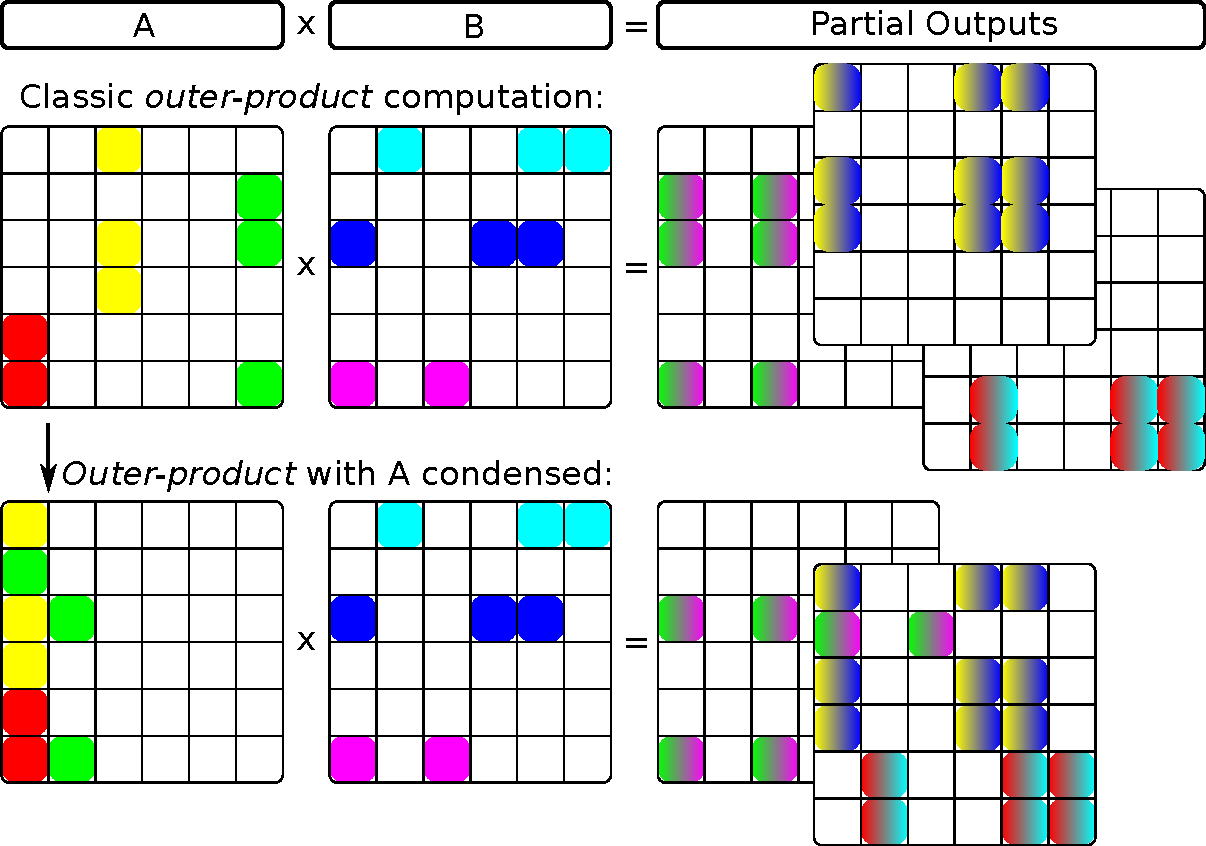
\includegraphics[width=0.85\linewidth]{Chapter_SoA/Figures/PDF/SpArch_algo.pdf}
            \caption{\emph{Outer-product} with a Condense $A$-Matrix}
            \label{fig:soa:sparch_algo}
        \end{figure}
    \end{minipage}
    \hfill
    \begin{minipage}[b]{0.44\linewidth}
        \begin{figure}[H]
            \centering
            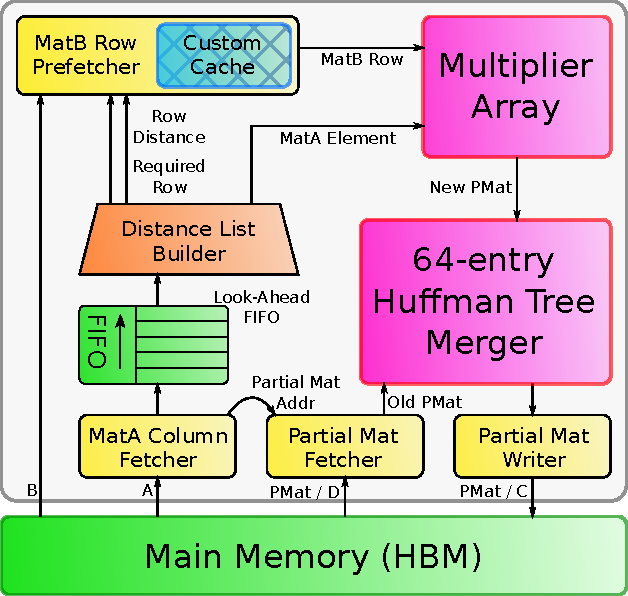
\includegraphics[width=0.8\linewidth]{Chapter_SoA/Figures/PDF/SpArch.pdf}
            \caption{Architecture of SpArch}
            \label{fig:soa:sparch}
        \end{figure}
    \end{minipage}
\end{figure}

% %%%%%%%%%%%%%%%%%%%%%%%%%%%%%%%%%%%%%%%%%%%%%%%%%%%%%%%%%%%%%%%%%%%%%
% %% State-of-the-Art %%
% MatRaptor
% %%%%%%%%%%%%%%%%%%%%%%%%%%%%%%%%%%%%%%%%%%%%%%%%%%%%%%%%%%%%%%%%%%%%%

\subsection{MatRaptor}
\label{sec:soa:matraptor}

MatRaptor~\cite{Srivastava2020_MatRaptor} is an accelerator designed to compute SpMSpM kernels. It is based on \algo{Gust} algorithm\footnote{Called \emph{row-wise product} in~\cite{Srivastava2020_MatRaptor}.}, which makes it possible to process multiple $A$-rows (2 to 8 for MatRaptor) in parallel. In MatRaptor (see Figure~\ref{fig:soa:matraptor}) a \emph{SpAL} (\emph{Sparse Matrix A Loader}) fetches non-zero elements of a $A$-row and sends them to a \emph{SpBL} (\emph{Sparse Matrix B Loader}). With the \emph{metadata} of this element, the \emph{SpBL} fetches non-zero elements of the corresponding $B$-rows and sends pairs of $A$- and $B$-elements to a \emph{PE}. This \emph{PE} computes the \emph{partial sums} and sends the results into queues for the \emph{merge} process. Instead of separating \emph{multiply} and \emph{merge} phases, several queues are used to store \emph{partial sums} and partially merged \emph{partial sums}, allowing the two phases to be pipelined. The \emph{PE} merges all the \emph{partial sums} resulting from an entire $A$-row, before sending the final output (the corresponding $C$-row) to main memory.

In MatRaptor, multiple $A$-rows are processed independently and in parallel in different \emph{PEs} and each \emph{PE} is assigned to a channel in an HBM memory~\cite{JESD235B}. It is important that each \emph{PE} can read its $A$-rows without interfering with the other \emph{PEs}. With the classic \emph{(UOP, CP) row-major} format, the rows are consecutive in memory and are not aligned to channel boundaries. To solve this problem, the authors propose a new format called \emph{C$^2$SR} (\emph{(FL, UOP, CP) channel-major}) that is based on a \emph{(UOP, CP) row-major}. For example, with two \emph{PEs}, all the elements of the even rows are stored in one channel, and the elements of the odd rows, in another channel, thus isolating the data. With this approach, the row pointers (\emph{UOP}) are no longer monotonic, which means that the length of a row can not be deduced by subtracting adjacent row pointers. This requires the addition of a new table (which we call \emph{fiber length} \emph{FL}), which stores the length of the non-zero elements in each row (see Figure~\ref{fig:soa:C2SR}). This modified storage format enables multiple \emph{PEs} to make effective use of the HBM.

MatRaptor is one of the first accelerators to use \algo{Gust} algorithm, however, it has some limitations regarding effective reuse of $B$-rows, both between parallel \emph{SpBLs} and temporally, as $A$ is traversed. A key contribution is the proposed \emph{C$^2$SR} input format, which makes it possible to separate rows into memory channels, to improve performance.

\begin{figure}
    \centering
    \begin{minipage}[b]{0.34\linewidth}
        \begin{figure}[H]
            \centering
            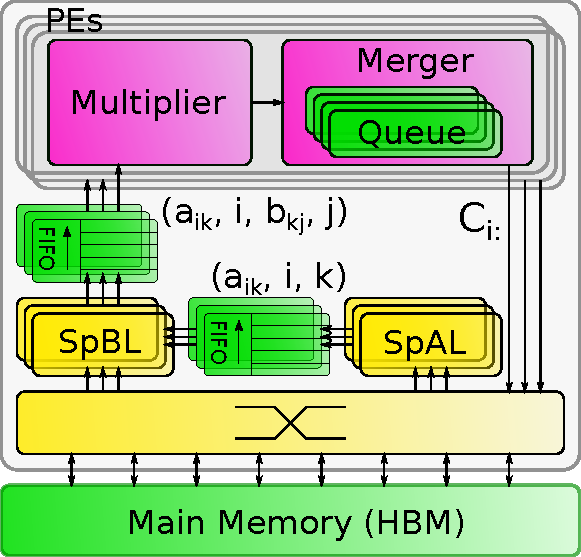
\includegraphics[width=0.85\textwidth]{Chapter_SoA/Figures/PDF/MatRaptor.pdf}
            \caption{Architecture of MatRaptor}
            \label{fig:soa:matraptor}
        \end{figure}
    \end{minipage}
    \hfill
    \begin{minipage}[b]{0.64\linewidth}
        \begin{figure}[H]
            \centering
            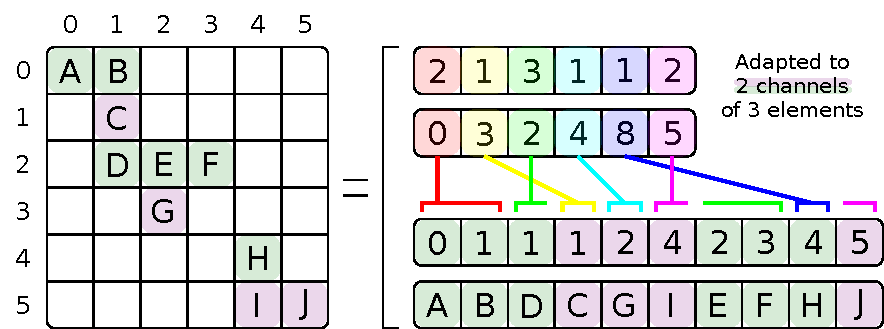
\includegraphics[width=0.9\textwidth]{Chapter_Background/Figures/PDF/SparseFormats/C2SR.pdf}
            \caption{\emph{(FL, UOP, CP) Channel-Major} Format ($C^{2}SR$)}
            \label{fig:soa:C2SR}
        \end{figure}
    \end{minipage}
\end{figure}

% %%%%%%%%%%%%%%%%%%%%%%%%%%%%%%%%%%%%%%%%%%%%%%%%%%%%%%%%%%%%%%%%%%%%%
% %% State-of-the-Art %%
% InnerSP
% %%%%%%%%%%%%%%%%%%%%%%%%%%%%%%%%%%%%%%%%%%%%%%%%%%%%%%%%%%%%%%%%%%%%%

\subsection{InnerSP}
\label{sec:soa:innersp}

InnerSP~\cite{Baek2021_InnerSP} is a SpMSpM accelerator based on the \algo{Gust} algorithm\footnote{The authors call this \emph{row-wise inner-product}, or confusingly sometimes \emph{inner-product}.}. The authors of InnerSP justify their choice by showing quantitatively that with the \algo{OP} the \emph{POs} represent a large volume of data, and that for many matrices the \emph{reductions} can not be done fully on-chip and thus must be buffered in main memory. Normally, with \algo{Gust} algorithm, $B$ must be read repeatedly, but InnerSP proposes a special cache for $B$ which exploits the spatial locality.

The architecture of InnerSP is shown in Figure~\ref{fig:soa:innersp}. The \emph{A reader} reads the $A$-rows. Two separate caches are used for $B$, one that stores the row pointers and the other which stores column indices and values. The \emph{B reader} reads the required $B$-rows, hopefully getting the data from the caches. Parallel multipliers perform the multiplications and then a hash-unit generates a hash based on the indices in $C$. A \emph{reduction} unit based on hash tables contains parallel comparators which search for matching hash values and performs the \emph {reductions}. When all the operations for a $A$-row are completed, the \emph{C writer} writes the $C$-row back to main memory.

% Figure located in Accelerators.tex

The architecture is efficient, as long as the \emph{Hash Reduction Unit} does not overflow. When overflows occur, the extra entries are temporarily stored in main memory, but there is a significant performance hit. To minimize the chance of overflows, InnerSP uses a pre-scanner to estimate the number of non-zero entries in the upcoming $C$-rows. The estimate primarily considers the $NNZ$ in the $A$-rows. If the estimated number of non-zero entries in $C$ exceeds the capacity of the \emph{Hash Reduction Unit}, then the row is split and processed in two passes. Conversely, if the number of non-zero entries in $C$ is small, two $A$-rows can be processed simultaneously.

To improve the performance of the $B$-cache, the authors exploit a technique from~\cite{Balaji2021_Popt}. The non-zero elements in the $A$-rows provide direct information about which $B$-rows are required. The column index table of $A$ is already pre-fetched by the \emph{A reader}, and when a row must be evicted from the $B$-cache, it chooses the ones which will not be required based on the upcoming entries in the column index table of $A$. This technique (also used by SpArch~\cite{Zhekai2020_SpArch}) maximizes the reuse of $B$-rows.

InnerSP is an accelerator based on \algo{Gust} algorithm which achieves high reuse of the $B$-rows, through a look-ahead in the $A$-\emph{metadata}.

\begin{figure}
    \centering
    \begin{minipage}[b]{0.54\linewidth}
        \begin{figure}[H]
            \centering
            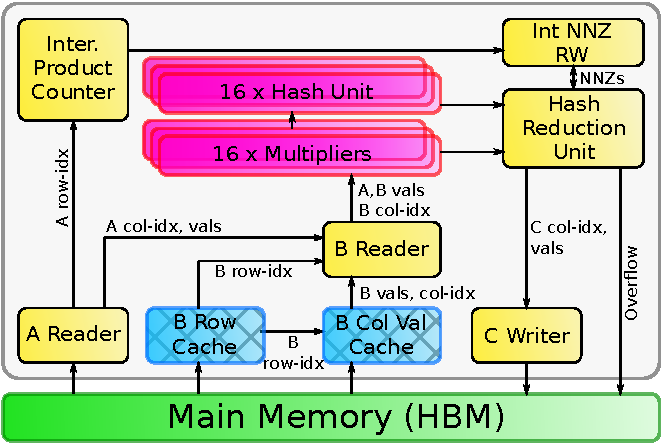
\includegraphics[width=0.9\textwidth]{Chapter_SoA/Figures/PDF/InnerSP.pdf}
            \caption{Architecture of InnerSP}
            \label{fig:soa:innersp}
        \end{figure}
    \end{minipage}
    \hfill
    \begin{minipage}[b]{0.44\linewidth}
        \begin{figure}[H]
            \centering
            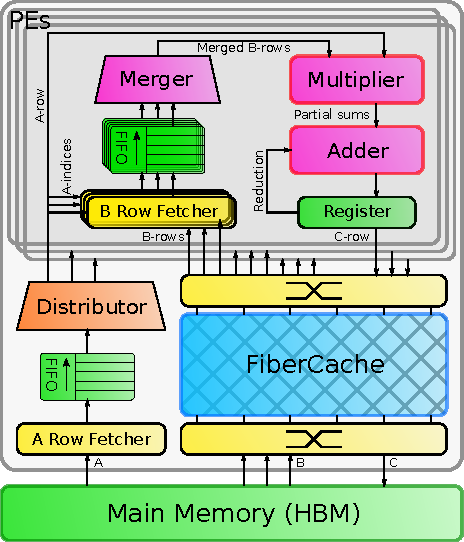
\includegraphics[width=0.8\textwidth]{Chapter_SoA/Figures/PDF/Gamma.pdf}
            \caption{Architecture of Gamma}
            \label{fig:soa:gamma}
        \end{figure}
    \end{minipage}
\end{figure}

% %%%%%%%%%%%%%%%%%%%%%%%%%%%%%%%%%%%%%%%%%%%%%%%%%%%%%%%%%%%%%%%%%%%%%
% %% State-of-the-Art %%
% Gamma
% %%%%%%%%%%%%%%%%%%%%%%%%%%%%%%%%%%%%%%%%%%%%%%%%%%%%%%%%%%%%%%%%%%%%%

\subsection{Gamma}
\label{sec:soa:gamma}

Gamma~\cite{Zhang2021_Gamma} is a dedicated accelerator for SpMSpM kernels, which uses \algo{Gust} algorithm. The two input matrices are both stored in \emph{(UOP, CP) row-major} format and the output is generated in the same format, providing consistency.

% Figure in Accelerators.tex

The Gamma architecture, presented in Figure~\ref{fig:soa:gamma}, is composed of a fetcher for the $A$-rows that contains a \emph{Distributor} to distribute them to 32 \emph{PEs}. Each \emph{PE} processes an entire $A$-row and computes the corresponding $C$-row. The \emph{PE} fetches the required $B$-rows and merges and sorts them in a 64-wide \emph{merge} block, before multiplying with the $A$-elements. As a result, the output $C$-row  is generated in order. The \emph{reduction} step is, thus, highly simplified, because any duplicate indices are adjacent. Normally, the $C$-row can be written back to main memory. However, if the $A$-row contains more than 64 non-zero elements, then it must be processed with multiple passes. After each pass, the partial $C$-row is stored temporarily. Finally, the temporary $C$-rows are read-back and merged by the \emph{PEs}.
Of course, the $B$-rows must be accessed repeatedly by the different \emph{PEs}, and Gamma proposes \emph{FiberCache} which is a highly banked cache which fetches the $B$-rows in advance, based on the column index table of $A$. It keeps track of which rows of $B$ are most needed by the \emph{PEs}, and when an eviction is necessary, the victim, is the row which is least needed.

Gamma encounters some difficulties when the $A$-matrix has rows that are too dense, requiring multiple iterations through the \emph{PEs}, which creates a high-load on the cache. The authors propose a software preprocessing technique which splits dense $A$-rows and rearranges them to make best use of the \emph{FiberCache}.

% Partial accelerators

% VL: SPiDRE and PHI here

% %%%%%%%%%%%%%%%%%%%%%%%%%%%%%%%%%%%%%%%%%%%%%%%%%%%%%%%%%%%%%%%%%%%%%
% %% State-of-the-Art %%
% SortCache
% %%%%%%%%%%%%%%%%%%%%%%%%%%%%%%%%%%%%%%%%%%%%%%%%%%%%%%%%%%%%%%%%%%%%%

\subsection{SortCache}
\label{sec:soa:sortcache}

The authors of SortCache~\cite{Srikanth2021_SortCache} note that modern processors are able to load an entire cache line in parallel but in many sparse applications less than 50\% of the data within a line is used, even with hand-tuned code. They propose a light SpGEMM accelerator which offloads the \emph{reduction} step, based on the \emph{Vectorized Binary Search Tree} (VBST), a data-structure from their earlier work~\cite{Srikanth2017_SuperStrider,Srikanth2019_MetaStrider}.
The VBST is a standard binary search tree where the size of node is a multiple of the cache block size and contains a sorted vector of $K$ $(key, value)$ pairs. Associated with each node is a \emph{pivot}; the pivots, with left and right child pointers, form a binary tree, as illustrated in Figure~\ref{fig:soa:sortcache_vbst}.

% Location of Figure in Accelerators.tex

Using the VBST, SortCache focuses on accelerating the \emph{scatter} updates to the output matrix, which are performed directly in the cache. The authors augment the processor with a single new instruction, \mbox{\emph{RED Key, Value}}. After $K$ updates have been issued, the hardware launches a \emph{reduction} in the SortCache, where the $K$ $(key, value)$ pairs are inserted into the VBST. This is done by traversing the tree from the root to the leaves. When duplicate keys are found, the \emph{reduction} operation is performed in the cache. When new keys are found, they are inserted, which can result in a temporary, new node with up to $2K$ $(key, value)$ pairs. This temporary node is partitioned, with one half having exactly $K$ entries. The insertion procedure may require visiting each level of the tree at least once ($\mathcal{O}(log(n)$) and it does not ensure the uniqueness of the keys, so at the end, an additional full traversal of the tree is required to remove duplicates.

The nodes closest to the root of the tree are accessed most frequently and are thus mapped to the caches closest to the processor. The authors propose to re-purpose cache tracking hardware (e.g. TAG values, LRU counters) to store the additional metadata (pivots, pointers). One of the difficulties with SortCache is that, in some cases, a large fraction of the VBST nodes are underutilized.

\begin{figure}
    \centering
    \begin{minipage}[b]{0.64\linewidth}
        \begin{figure}[H]
            \centering
            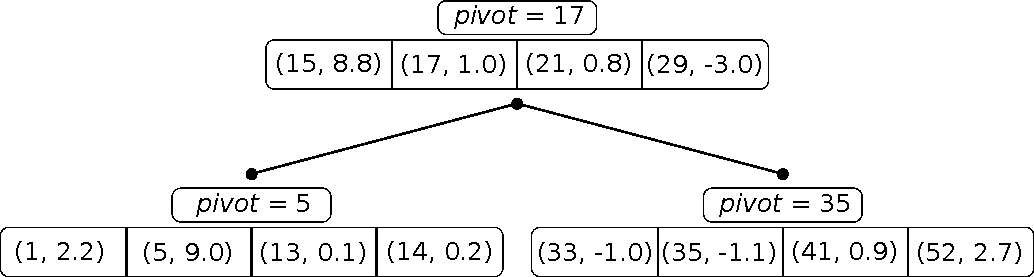
\includegraphics[width=\textwidth]{Chapter_SoA/Figures/PDF/VBST_example.pdf}
            \caption{VBST Data Structure Used by SortCache}
            \label{fig:soa:sortcache_vbst}
        \end{figure}
    \end{minipage}
    \hfill
    \begin{minipage}[b]{0.34\linewidth}
        \begin{figure}[H]
            \centering
            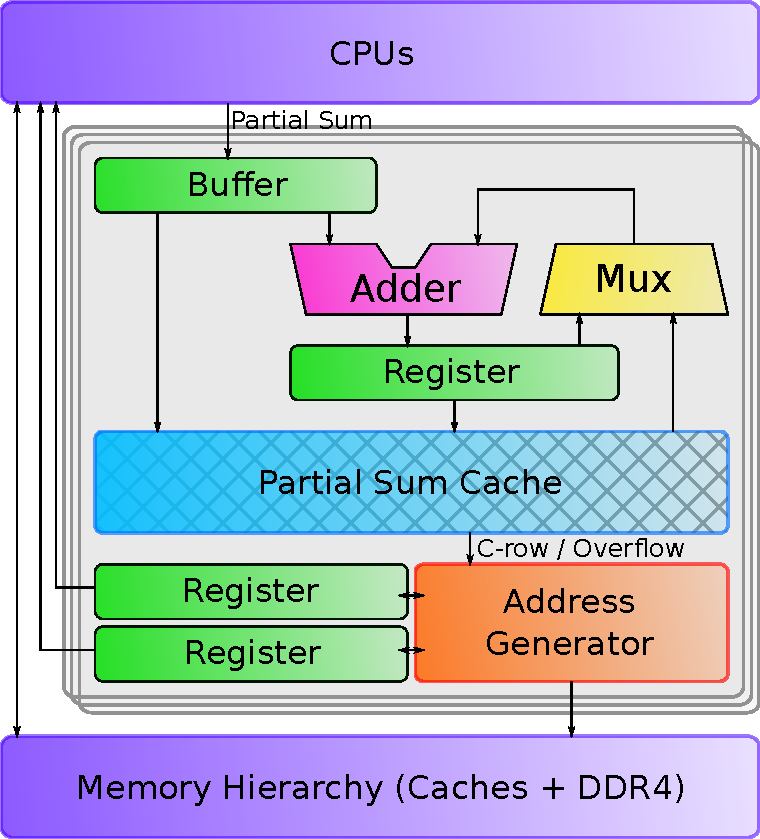
\includegraphics[width=\textwidth]{Chapter_SoA/Figures/PDF/ASA.pdf}
            \caption{Architecture of ASA}
            \label{fig:soa:asa}
        \end{figure}
    \end{minipage}
\end{figure}

% %%%%%%%%%%%%%%%%%%%%%%%%%%%%%%%%%%%%%%%%%%%%%%%%%%%%%%%%%%%%%%%%%%%%%
% %% State-of-the-Art %%
% ASA
% %%%%%%%%%%%%%%%%%%%%%%%%%%%%%%%%%%%%%%%%%%%%%%%%%%%%%%%%%%%%%%%%%%%%%

\subsection{ASA}
\label{sec:soa:asa}

In the scope of graph analytic problems, the authors of ASA~\cite{Zhang2022_ASA} observed that \algo{Gust} algorithm achieves high performance for SpGEMM kernels but note that it still requires acceleration for the \emph{reduction} step\footnote{The authors refer to the \emph{reduction} step as SPA (Sparse Accumulation).}. The software state-of-the-art for \emph{reduction} uses hash tables~\cite{Brock2021_GraphBLAS}. Some hardware accelerators, such as HTA~\cite{Zhang2019_HTA}, enhance performance for hash operations, but those solutions are not optimized for SpGEMM kernels. ASA is a low area, near-core extension for a general purpose processor that specifically accelerates the \emph{reduction} step for \algo{Gust} algorithm.

ASA accelerates \emph{reduction} operations received from software via custom instructions.
As presented in Figure~\ref{fig:soa:asa}, the \emph{partial sums} from these instructions are stored in a waiting buffer as $(index, value)$ pairs with a key that is a hash of the index, computed in software to maintain flexibility. The cache line, accessed with the key, is filled with the indices and the \emph{partial sums}. If a corresponding \emph{partial sum} is already stored, ASA accumulates it and writes back the result. If not, the \emph{partial sum} is simply stored into the cache. 

To minimize die area, the cache is not dimensioned for an entire $C$-row\footnote{The authors present a \emph{column-wise} \algo{Gust} implementation. This choice is arbitrary and, for consistency, we stick with a \emph{row-wise} presentation.} but ASA handles cache overflows in hardware. When a \emph{partial sum} needs to be stored in a fully filled cache line, a victim is selected and evicted, based on a LRU policy. The evicted entry is written into a pre-allocated FIFO queue in the memory hierarchy. ASA uses an address generator to manage evicted data and updates head and tail registers for the list. Software then traverses the list to merge duplicate keys to build the final output $C$-row. To avoid overflows, the authors advocate \emph{tiling} methods to efficiently distribute work through one or several ASA cores.

% Figure in Accelerators.tex

ASA is an accelerator which  optimizes the \emph{scatter} aspect of SpGEMM kernel with low area overhead, while leaving high software flexibility. Unlike other \algo{Gust} accelerators, there is no hardware \emph{gather} support for reusing or caching the $B$-rows.

%%%%%%%%%%%%%%%%%%%%%%%%%%%%%%%%%%%%%%%%%%%%%%%%%%%%%%%%%%%%%%%%
% Other Accelerators
%%%%%%%%%%%%%%%%%%%%%%%%%%%%%%%%%%%%%%%%%%%%%%%%%%%%%%%%%%%%%%%%
\subsection{Other Accelerators}
\label{sec:soa:other_accel}

In the above sections, we have described a selection of the main sparse accelerators that have appeared in the literature, covering different matrix multiplication algorithms and architectures. This list is not exhaustive, and in the following paragraphs we present several other accelerators which we will cover in less detail, due to space constraints.

\subsubsection{SPiDRE}

The authors of SPiDRE (Sparse Data Rearrange Engine)~\cite{Barredo2019_SPiDRE} propose a solution for the poor utilization of the memory hierarchy in sparse applications. They propose a near-memory data rearrangement engine. This engine can preprocess data, near memory, to create new data-structures that are dense and benefit from the memory hierarchy. For example, with a SpMV kernel, the input vector could be rearranged through a user defined function to a dense format where all non-zero elements are in the right order of computation.

\subsubsection{PHI}

The authors of PHI~\cite{Mukkara2019_PHI} note that many large graph algorithms favour pull (each node reads inputs from its neighbours) compared to push implementations (each node propagates results to its neighbours), as push implementations require read-modify-writes which require accessing complete cache lines, even though a small unit of data is modified. The authors include \algo{OP} SpMV (a push algorithm) in their evaluation.

PHI is a modified cache optimized to efficiently process commutative \emph{scatter} updates. When an update is received but the line is not in the cache, the line is not fetched, but rather marked as being in \emph{update mode}, where it simply stores the update. If subsequent updates hit the line, they are stored, or combined via the commutative operator. When a cache line is evicted, if it contains multiple updates, PHI assumes that the coalescing has been effective, and it processes the operations via a read-modify-write from main memory. If a cache contains few updates when evicted, PHI batches these updates as $(address, value)$ tuples, allocating a new cache line to assemble the batch. Groups of updates are organized by \emph{bins} corresponding to a small memory region. The batches are streamed to main memory. Later, the reading of the batches is also efficient, as they are contiguous.

In multi-core systems, private caches act as local buffers, thus coalescing the updates reduces coherency protocol traffic. This combination of in-cache coalescing and update buffering enables PHI to take advantage of locality when possible (like Coup~\cite{ZHANG_2015__Exploiting_Commutativity}), but with the addition of \emph{update batching}, PHI improves memory utilization, even when the data being updated is too large to fit in the cache.

\subsubsection{GSCSp}

GSCSp~\cite{LI_2023_GSCSp} is a FPGA-based accelerator based on \algo{Gust} algorithm. In other \algo{Gust} accelerators, a \emph{PE} processes a full $A$-row but the authors note that when there is variability in the number of elements in the $A$-rows, \emph{PEs} may be blocked, waiting for another \emph{PE} to complete. Thus the authors propose to distribute the elements in an $A$-row to different \emph{PEs} (\emph{element-wise} parallelism). Initially, each \emph{PE} buffers its output $C$-row, and when a \emph{PE} advances to the next row, it pushes its partial $C$-row to a final merger. The authors also propose to use separate caches for the \emph{metadata} for the $B$-rows and the values, and report that combined with the \emph{element-wise} parallelism, the approach is effective for reducing the memory traffic for accessing $B$-rows.

\subsubsection{Flexagon}

Flexagon~\cite{Munoz-Martinez2023_Flexagon} is a SpMSpM accelerator for DNN applications. The authors claim that the optimal algorithm (\algo{IP}, \algo{OP} and \algo{Gust}) depends on the matrix structure, potentially varying between DNN models and layers within a DNN, although in the majority of the cases, their data shows that \algo{Gust} is the most efficient. Flexagon is configurable: it can implement all three  algorithms. To achieve that, the authors designed a \emph{Merger-Reduction Network} (\emph{MRN}) that is able to perform multiplications (for \emph{partial sum} generation), accumulations (for \emph{reductions} operations) and comparisons (for \emph{intersection} searches and \emph{merge} phases) via a binary tree structure. Flexagon addresses the memory access issues of each algorithms via three custom memories: a FIFO for the $A$-matrix that is always read sequentially, a cache for the $B$-matrix that is subject to high temporal and spatial reuse in each of the three algorithms, and a PSRAM to store \emph{POs} for \algo{OP} and \algo{Gust} algorithms.

\subsubsection{Other Accelerators}

In GraphR~\cite{Song2018_GraphR}, the authors propose to use ReRAM technology and a cross-bar to perform graph operations directly in hardware, but this approach is not currently scalable to large problems. The ITS accelerator~\cite{Sadi2019_ITS} focuses on an \algo{OP} implementation of SpMV and they apply data-compression to the \emph{metadata}. The authors of SPU~\cite{Dadu2019_SPU} propose a more general hardware solution to input data dependencies and focus on graph applications. The focus of Alrescha~\cite{Asgari2020_Alrescha} is an innovative and adaptive preprocessing of the matrix in hardware to simplify the accesses to the $b$-vector. The authors of CoSparse~\cite{Feng2021_CoSPARSE} focus on a software layer that selects the hardware acceleration that is best adapted to the given problem.

The SSSR accelerator~\cite{Scheffler2023_SSSR} for RISC-V processors goes further by addressing \emph{intersection} and \emph{union} while streaming data to and from memory and it can be used for multiple kernels, however the RISC-V performance can not easily be compared with the other accelerators presented in this paper. In passing we note three other accelerators EIE~\cite{Han2016_EIE}, SCNN~\cite{Angshuman2017_SCNN} and CANDLES~\cite{Gudaparthi2022_CANDLES} which have hardware support for sparsity but which are highly focused on CNNs, besides SDMA~\cite{Gao2023_SDMA} that focuses on GNNs.

The SpaceA~\cite{Xie2021_SpaceA} accelerator exploits near-memory computing inside a 3D DRAM memory to implement SpMV using an \algo{IP} algorithm. With preprocessing, the rows of the matrix are assigned to banks within specific DRAM dies, while optimizing spatial locality. A separate die is used for storing the input and output vectors. Associated with each DRAM bank which stores the matrix, there is a \emph{PE} which reads the non-zero values of the matrix, fetches the required vector entries and performs the computations. Bringing the compute near the DRAM and exploiting emerging 3D technology, is an orthogonal approach to reduce memory access overheads.

\subsubsection{Other FPGA based Accelerators}

Many sparse accelerators have been prototyped on FPGAs~\cite{MOHAMMED_2022_SPARSE}. Indeed, AMD/Xilinx provide a turnkey library for SpMV~\cite{Xilinx_Vitis_2021, Li2023_OnXilinx}. In \cite{Du2022_HiSparse}, the authors propose a higher-performance SpMV using a modified \emph{CSR} format where the data is packed for efficient, streaming access in HBM\footnote{GraphLily~\cite{Hu2021_GraphLily} is a precursor of HiSparse, also from Cornell University.}. They also propose a highly-banked on-chip memory for the vector updates, and a hazard resolution strategy that allows efficient pipelining.

% %%%%%%%%%%%%%%%%%%%%%%%%%%%%%%%%%%%%%%%%%%%%%%%%%%%%%%%%%%%%%%%%%%%%%
% Comparison and Analysis
% %%%%%%%%%%%%%%%%%%%%%%%%%%%%%%%%%%%%%%%%%%%%%%%%%%%%%%%%%%%%%%%%%%%%%

\section{Comparison of Existing Accelerators}
\label{sec:soa:comparison_and_analysis}

In this section, we analyze and further compare the accelerators that were described in Section~\ref{sec:soa:hw_accelerators}. We start with Table~\ref{tab:soa:classificationMaturity} where we summarize the accelerators, chronologically, showing the research group where they were developed. We see that MIT is very active in the field, as they were involved in developing four different accelerators (\emph{e.g.} ExTensor, PHI, SpArch and Gamma).

\begin{table}
    \caption{Chronological Summary of Sparse Accelerators}
    \centering
    \footnotesize
    \begin{tabular}{|c|c|| >{\centering\arraybackslash}m{4.05cm}|| >{\centering\arraybackslash}m{7.19cm}|}
        \hhline{--||-||-}
        \textbf{Name} & \textbf{Date} & \textbf{Institute / University} & \textbf{Summary} \\
        \hhline{==::=::=}
        OuterSPACE~\cite{Pal2018_OuterSPACE} & 2018 & Univ. of Michigan / Arizona State Univ. & Highly parallelized SPMD, two levels cache -- \algo{OP} SpMSpM \\
        \hhline{--||-||-}
        ExTensor~\cite{Hegde2019_ExTensor} & 2019 & Univ. of Illinois / NVIDIA / MIT & General purpose tensor algebra -- With \emph{tiled} SpMSpM \\
        \hhline{--||-||-}
        PHI~\cite{Mukkara2019_PHI} & 2019 & MIT (CSAIL) / Carnegie Mellon Univ. & In cache, hash-based accelerator for \emph{reductions} \\
        \hhline{--||-||-}
        SPiDRE~\cite{Barredo2019_SPiDRE} & 2019 & UPC, BSC (Spain) / Arm Research & Near main memory data reorganisation for \emph{intersections} \\
        \hhline{--||-||-}
        MatRaptor~\cite{Srivastava2020_MatRaptor} & 2020 & Cornell & Row-parallel with HBM-aware custom format -- \algo{Gust} SpMSpM \\
        \hhline{--||-||-}
        SpArch~\cite{Zhekai2020_SpArch} & 2020 & MIT / Stanford / NVIDIA & Compression method to reduce \emph{POs}, \emph{multiply}/\emph{merge} pipe -- \algo{OP} SpGEMM \\
        \hhline{--||-||-}
        SpaceA~\cite{Xie2021_SpaceA} & 2021 & UC Santa Barbara & In memory accelerator for 3D DRAM -- \algo{IP} SpMV \\
        \hhline{--||-||-}
        Gamma~\cite{Zhang2021_Gamma} & 2021 & MIT (CSAIL) & Parallelized architecture with \emph{FiberCache} for $B$ -- \algo{Gust} SpMSpM \\
        \hhline{--||-||-}
        InnerSP~\cite{Baek2021_InnerSP} & 2021 & KAIST / DGIST (S. Korea) & $A$-look-ahead, caches for $B$, \emph{Hash Reduction Unit} for $C$ -- \algo{Gust} SpMSpM \\
        \hhline{--||-||-}
        SortCache~\cite{Srikanth2021_SortCache} & 2021 & Georgia Tech / Zettaflops / Sandia Labs & In cache accelerator for \emph{reductions}, based on the VBST \\
        \hhline{--||-||-}
        ASA~\cite{Zhang2022_ASA} & 2022 & Lehigh Univ. / Lawrence Berkeley & Custom cache accelerator for \emph{reductions} -- \algo{Gust} SpGEMM \\
        \hhline{--||-||-}
        Flexagon~\cite{Munoz-Martinez2023_Flexagon} & 2023 & Univ. of Murcia / Georgia Tech / NVIDIA & Configurable accelerator supporting all three algorithms -- SpMSpM \\
        \hhline{--||-||-}
        GSCSp~\cite{LI_2023_GSCSp} & 2023 & Nanyang Technological Univ. & Element-wise, FPGA-based accelerator -- \algo{Gust} SpMSpM \\
        \hhline{--||-||-}
    \end{tabular}
    \label{tab:soa:classificationMaturity}
\end{table}

\subsection{Benchmarks, Evaluation and Performance}

Up to this point, we have discussed the architecture of the various accelerators, without reporting the performance they achieve.
Most of the matrices used for benchmarking come from the SuiteSparse Matrix Collection~\cite{Kolodziej2019_SuiteSparse} that contains a large number of matrices from diverse, real applications. Domain specific matrix libraries are also used~\cite{Leskovec2014_SNAP, Smith2017_FROSTT, Azad2018_HipMCL, Reddi2020_MLPerf}, as well as some synthetic matrix generators~\cite{Ang2010_Graph500, Beamer2017_GAP}.
The densities are in general less than 1\% and can be as low as $10^{-5}$\%. ExTensor, SortCache and Flexagon also benchmark with denser matrices. In all cases, large matrices with several million $NNZ$, exceeding the size of a normal cache, have been evaluated.

\begin{table}
    \centering
    \caption{Qualitative Analysis and Evaluation of Sparse Accelerators}
    \footnotesize
    \begin{tabular}{|c|| >{\centering\arraybackslash}m{1.97cm}| >{\centering\arraybackslash}m{7.17cm}| >{\centering\arraybackslash}m{2.7cm}|}
        \hhline{-||---}
        \textbf{Name} & \textbf{Preprocessing\hyperlink{fn101}{$^{1}$}} & \textbf{Functional Evaluation (Tool / Evaluation Specifics / Host\hyperlink{fn102}{$^{2}$})} & \textbf{Local Memory Size} \\
        \hhline{=::===}
        OuterSPACE~\cite{Pal2018_OuterSPACE} & $A$ $\rightarrow$ \emph{row-major} & \emph{gem5} / Model only key elements; Skip memory allocation; Ignore start-up time / $\varnothing$ & 528KiB (33.8k entries) \\ % 1kB * 16 * 16 + 16kB * 16 + 4kB * 4 = 528kB -> 33ki elements (33.8k)
        \hhline{-||---}
        ExTensor~\cite{Hegde2019_ExTensor} & $A$, $B$ $\rightarrow$ highly \emph{tiled} custom format & Custom Python simulator / Only the \emph{Coordinator} is evaluated; Remainder modeled analytically / $\varnothing$ & $\sim$38MiB (2.5M entries) \\ % 64kB * 128 + 30MB + ? = ~ 38MB -> ~ 2.4Mi elements (2.5M)
        \hhline{-||---}
        PHI~\cite{Mukkara2019_PHI} & \emph{N/A} & \emph{ZSim} / Entirely evaluated / 16-cores system with 3 level cache & 32.3MiB (2.8M entries) \\ % 32kB + 256kB + 32MB = 32.3MB -> 2.7Mi elements (2.8M)
        \hhline{-||---}
        SPiDRE~\cite{Barredo2019_SPiDRE} & Not needed & \emph{gem5} / \emph{Unknown} / Single ARM core & $\varnothing$ (main memory size) \\ % no data but works in main memory
        \hhline{-||---}
        MatRaptor~\cite{Srivastava2020_MatRaptor} & $A$, $B$ $\rightarrow$ \emph{C$^2$SR} & \emph{gem5} / Entirely evaluated / $\varnothing$ & 320KiB (27.3k entries) \\ % 8 * 10 * 4KB = 320kB -> 26.7ki elements (27.3k)
        \hhline{-||---}
        SpArch~\cite{Zhekai2020_SpArch} & $A$, $B$ $\rightarrow$ \emph{row-major} & Custom C++ simulator / Entirely evaluated / $\varnothing$ & 940KiB (62.5k entries) \\ % 1024 * 12B + 1024 * 48 * 12B + 8192 * 12B + 16*16*16B(array) * 64 = 940kB -> 61ki element (62.5k)
        \hhline{-||---}
        SpaceA~\cite{Xie2021_SpaceA} & $A$ $\rightarrow$ row-aligned to DRAM banks & Custom simulator / Simulation tracking values stored in 3D-DRAM / $\varnothing$ & 4GiB (268.4M entries) \\ % 4GB -> 256Mi elements (268.4M)
        \hhline{-||---}
        Gamma~\cite{Zhang2021_Gamma} & $A$, $B$ $\rightarrow$ \emph{row-major} & Custom simulator / Entirely evaluated / $\varnothing$ & 3MiB (262.1k entries) \\ % 3MB -> 256ki elements (262,1k)
        \hhline{-||---}
        InnerSP~\cite{Baek2021_InnerSP} & Not needed & Custom simulator / Entirely evaluated / $\varnothing$ & $\leq$976.5KiB (119.9k entries) \\ % 4B * 1024 + 12B * 4096 + 8B * 1024 + 12B * 128 * 64 + 32kB (/8) + 256(or512)kB (/8) + 2 * 4B * 1024 + 16 * 16kB (/8) + 4B * 128 + 12B * 1024 = 720.5kB -> 85.1ki elements (87.2k) OR 976.5kB -> 117.1ki elements (119.9k)
        \hhline{-||---}
        SortCache~\cite{Srikanth2021_SortCache} & \emph{N/A} & Custom simulator / Entirely evaluated / Single threaded, in-order core  with 3 level cache & 16.3MiB (1.4M entries) \\ % 32kB + 256kB + 16MB = 16.3MB -> 1.4Mi elements (1.4M)
        \hhline{-||---}
        ASA~\cite{Zhang2022_ASA} & \emph{N/A} & Modified \emph{ZSim} / Entirely evaluated, one ASA per core / 8-cores with 3 level cache & 8$\times$8KiB (8$\times$1k entries) \\ % for one ASA: 8kB -> 1ki elements (1k)
        \hhline{-||---}
        Flexagon~\cite{Munoz-Martinez2023_Flexagon} & Not needed & Custom simulator based on STONNE / Entirely evaluated / $\varnothing$ & 1.3MiB (327.7k entries) \\ % open source soon // 256B + 1MB + 256KB (/4B) = 1.3MB -> 320.1ki elements (327.7k)
        \hhline{-||---}
        GSCSp~\cite{LI_2023_GSCSp} & $A$, $B$ $\rightarrow$ \emph{row-major} & HLS / FPGA Prototype / $\varnothing$ & 2.1MiB (178.2k entries) \\ % 40kB + 2MB = 2.1MB -> 174ki elements (178.2k)
        \hhline{-||---}
        \multicolumn{4}{l}{\hypertarget{fn101}{$^{1}$}We assume matrices are initially stored in \emph{(UOP, CP) column-major} format (\emph{CSC}).} \\
        \multicolumn{4}{l}{\hypertarget{fn102}{$^{2}$}Only for \emph{processor assist} accelerators.}
    \end{tabular}
    \label{tab:soa:evaluation}
\end{table}

% \begin{table}
%     \caption{Benchmark Matrices for Sparse MM and MV}
%     \begin{center}
%         \small
%         \begin{tabular}{|c||c|c|c|c|}
%             \hhline{-||----}
%             \textbf{Name} & \textbf{\# Matrices} & \textbf{Density Range} & \textbf{Largest NNZ} & \textbf{Sources} \\
%             \hhline{=::====}
%             \multirow{2}{*}{OuterSPACE~\cite{Pal2018_OuterSPACE}} & 20 & from 0.0001\% to 1.082\% & 16,518,948 & SuiteSparse and SNAP \\
%             \cline{2-5}
%             & \textit{unknown} & \textit{unknown} & \textit{unknown} & Graph500 R-MAT synthetic matrices \\
%             \hhline{-||----}
%             ExTensor~\cite{Hegde2019_ExTensor} & 14 & from 0.0002\% to 20.3\% & 11,524,432 & SuiteSparse and FROSTT \\
%             \hhline{-||----}
%             PHI~\cite{Mukkara2019_PHI} & 1 & 0.0001\% & 1,949,412,601 & SuiteSparse \\
%             \hhline{-||----}
%             SPiDRE~\cite{Barredo2019_SPiDRE} & \textit{unknown} & \textit{unknown} & \textit{unknown} & \textit{unknown} \\
%             \hhline{-||----}
%             MatRaptor~\cite{Srivastava2020_MatRaptor} & 14 & from 0.00061\% to 1.1\% & 5,105,039 & same as OuterSPACE \\
%             \hhline{-||----}
%             SpArch~\cite{Zhekai2020_SpArch} & 20 & from 0.0001\% to 1.082\% & 16,518,948 & same as OuterSPACE \\
%             \hhline{-||----}
%             SpaceA~\cite{Xie2021_SpaceA} & 15 & from 0.0003\% to 0.347\% & 14,148,858 & SuiteSparse \\
%             \hhline{-||----}
%             Gamma~\cite{Zhang2021_Gamma} & 37 & from 0.0001\% to 1\% & 16,518,948 & same as OuterSPACE plus SuiteSparse \\
%             \hhline{-||----}
%             \multirow{2}{*}{InnerSP~\cite{Baek2021_InnerSP}} & set of 755 & \textit{unknown} & 5,105,039 & SuiteSparse and SNAP \\
%             \cline{2-5}
%             & 14 & from 0.00061\% to 1.1\% & 5,105,039 & from OuterSPACE \\
%             \hhline{-||----}
%             SortCache~\cite{Srikanth2021_SortCache} & 11 & from 0.4\% to 78.5\% & 2,097,566 & SuiteSparse \\
%             \hhline{-||----}
%             ASA~\cite{Zhang2022_ASA} & 9 & from 0.00002\% to 0.3\% & $\sim$104,000,000 & HipMCL, SNAP and GAP \\
%             \hhline{-||----}
%             Flexagon~\cite{Munoz-Martinez2023_Flexagon} & 9 & from 6\% to 100\% & 2,718,144 & MLPerf \\
%             \hhline{-||----}
%             GSCSp~\cite{LI_2023_GSCSp} & 10 & from 0.09\% to 2.80\% & 484,256 & SuiteSparse \\
%             \hhline{-||----}
%         \end{tabular}
%         \label{tab:classificationMatrices}
%     \end{center}
% \end{table}

In Table~\ref{tab:soa:evaluation}, we note any required preprocessing, assuming, arbitrarily, that matrices are initially stored in \emph{CSC} format\footnote{This choice is based on the SuiteSparse Matrix Collection where matrices are stored \emph{column-major}.}. We see that a few accelerators require a conversion to their  specific format (\emph{e.g.} ExTensor and MatRaptor). PHI, SortCache and ASA are not concerned by preprocessing since they only address \emph{scatter}. In any case, fair benchmarking must take into account the cost of specialised preprocessing.

Not all accelerators have reached the same level of design maturity, and in Table~\ref{tab:soa:evaluation}, we have shown how each design was analyzed or simulated.
All designs report that they have been simulated at a cycle-accurate level. Most of the accelerators use custom simulators or tools like \emph{gem5}~\cite{Lowe2020_gem5}, \emph{ZSim}~\cite{SANCHEZ_2013_ZSIM} and STONNE~\cite{Munoz-Martinez2021_STONNE}, but unfortunately there is no common approach, making it difficult to fairly compare the reported performance. RTL descriptions are often only generated for key parts of the design. To estimate power and area, authors used tools such as CACTI~\cite{Balasubramonian2017_CACTI7} and McPAT~\cite{Li2009_McPAT}\footnote{We have not attempted to compare power/energy as the data in the literature is heterogeneous and can not be fairly compared.}.
In the last column of the table, we show the size of the local memory storage used in simulation by each accelerator. Except for SPiDRE and SpaceA which work directly in main memory, the local memories are in the range of 0.3MiB to 38MiB, corresponding to 27k to 2.8M entries. Thus, in the model presented in Section~\ref{sec:bg:AnalyticalModel}, most of the accelerators are situated in the middle-row of Figure~\ref{fig:bg:AnalyticalModel_SpMSpM}, with a local memory corresponding to a few matrix rows.

The accelerators performance are reported as a speedup versus a baseline, which may differ according to their hardware and software platforms: typically the Intel MKL library~\cite{Intel2003_IntelMKL} and the Armadillo library~\cite{Conrad2016_Armadillo} for CPUs, or cuSPARSE~\cite{NVIDIA2014_cuSPARSE} and CUSP~\cite{Dalton2014_Cusp} for GPUs.
Since different baselines with different numbers of threads and cores are used, these speedups need to be interpreted with care.
The speedups are in general higher for the \emph{standalone} accelerators as they provide optimized hardware for the entire kernel, while \emph{processor assist} accelerators have less impressive speedups but aim to be general purpose and have lower area overhead.

The only accelerators that have a comparable baseline are the \emph{standalone} ones addressing SpMSpM. They all compare themselves to OuterSPACE with the same benchmark matrices, so we can sort them by their speedup: Gamma ($6.6\times$)\footnote{This speedup increases to $7.7\times$ with their proposed preprocessing.}, InnerSP ($4.57\times$), SpArch ($4\times$), MatRaptor ($1.8\times$) and OuterSPACE ($1\times$).
Three of the five \emph{standalone} accelerators use the \algo{Gust} algorithm (Gamma, InnerSP and MatRaptor). SpArch, an \algo{OP} accelerator employing a complex architecture, outperforms MatRaptor, but does not achieve the same performance as InnerSP or Gamma, which suggests that \algo{Gust} is most adapted to high-performance hardware accelerators.

These measurements are consistent with our model presented in Section~\ref{sec:bg:AnalyticalModel} (Figure~\ref{fig:bg:AnalyticalModel_SpMSpM}). OuterSPACE, the baseline, corresponds to graph~\ding{196}. MatRaptor, the first \algo{Gust} accelerator, was able to achieve higher performance by reducing the number of \emph{random} accesses, and creating better regularity (red to yellow), as seen in graph~\ding{197}.

SpArch, is an \algo{OP} accelerator with a much larger local memory, which is used to address the red region in graph~\ding{196}. Their $A$-matrix condensing method, allows them to reduce the number of \emph{POs}, and approach the performance achievable in graph~\ding{199}, although, \emph{in fine}, it is impossible to store all the \emph{POs} in local memory. InnerSP and Gamma correspond to optimizations of the \algo{Gust} approach in graph~\ding{197}, to approach the performance in graph~\ding{200}. This is achieved by custom caches for the $B$-matrix to address the orange region. With the \algo{Gust} algorithm, it is only necessary to store a limited number of $B$-rows, which is achievable with the large local memories in these accelerators. The model presented in Section~\ref{sec:bg:AnalyticalModel} is helpful to understand the local memory requirements for SpMSpM accelerators.

%% RV %%
% \begin{table}
%     \caption{Reported Performance of Sparse Accelerators}
%     \begin{center}
%         \footnotesize
%         \begin{tabular}{|c|c|| >{\centering\arraybackslash}m{7cm} |c|c|c|}
%             \hhline{--||----}
%             & & \multicolumn{2}{c|}{\textbf{Baseline for Comparison}} & & \textbf{Average} \\
%             \cline{3-4}
%             \textbf{Name} & \textbf{Date} & \textbf{Hardware} & \textbf{Software} & \textbf{Kernels} & \textbf{Speedups} \\
%             \hhline{==::====}
%             %
%             \multirow{3}{*}{OuterSPACE} & \multirow{3}{*}{2018} & 6 cores/12 threads, 3.6 GHz Intel Xeon E5-1650V4 CPU & Intel MKL & \multirow{3}{*}{SpMV, SpMSpM} & \mbox{7.9$\times$} \\
%             \cline{3-4} \cline{6-6}
%             & & \multirow{2}{*}{NVIDIA Tesla K40 GPU} & cuSPARSE & & \mbox{1.13$\times$} \\
%             \cline{4-4} \cline{6-6}
%             & & & CUSP & & \mbox{1.14$\times$} \\
%             \hhline{==::====}
%             %
%             \multirow{2}{*}{ExTensor} & \multirow{2}{*}{2019} & \multirow{2}{*}{12 cores/24 threads, 3 GHz Intel Xeon E5-2687W v4 part} & \multirow{2}{*}{Intel MKL} & SpMSpM & \mbox{3.4$\times$} \\
%             \cline{5-6}
%             & & & & SpMM & \mbox{1.3$\times$} \\
%             \hhline{==::====}
%             %
%             \multirow{2}{*}{PHI} & \multirow{2}{*}{2019} & \multirow{2}{*}{2.2 GHz, 16 core x86-64 system} & outer-product & \multirow{2}{*}{SpMV} & \mbox{7$\times$} \\
%             \cline{4-4} \cline{6-6}
%             & & & inner-product & & \mbox{1.4$\times$} \\
%             \hhline{==::====}
%             %
%             SPiDRE & 2019 & single out-of-order Arm processor & \textit{unknown} & SpMV & \mbox{1.62$\times$} \\
%             \hhline{==::====}
%             %
%             \multirow{4}{*}{MatRaptor} & \multirow{4}{*}{2020} & single-threaded, 2.20 GHz Intel Xeon E5-2699 v4 server-class CPU & \multirow{2}{*}{Intel MKL} & \multirow{4}{*}{SpMSpM} & \mbox{77.5$\times$} \\
%             \cline{3-3} \cline{6-6}
%             & & 12 threads, 2.20 GHz Intel Xeon E5-2699 v4 server-class CPU & & & \mbox{7.9$\times$} \\
%             \cline{3-4} \cline{6-6}
%             & & NVIDIA Titan Xp GPU & cuSPARSE & & \mbox{37.6$\times$} \\
%             \cline{3-4} \cline{6-6}
%             & & OuterSPACE & $\varnothing$ & & \mbox{1.8$\times$} \\
%             \hhline{==::====}
%             %
%             \multirow{5}{*}{SpArch} & \multirow{5}{*}{2020} & 4-core ARM A53 CPU & Armadillo & \multirow{5}{*}{SpMSpM} & \mbox{1285$\times$} \\
%             \cline{3-4} \cline{6-6}
%             & & 6-core Intel Core-i7 5930K CPU & Intel MKL & & \mbox{19$\times$} \\
%             \cline{3-4} \cline{6-6}
%             & & \multirow{2}{*}{NVIDIA TITAN Xp GPU} & cuSPARSE & & \mbox{18$\times$} \\
%             \cline{4-4} \cline{6-6}
%             & & & CUSP & & \mbox{17$\times$} \\
%             \cline{3-4} \cline{6-6}
%             & & OuterSPACE & $\varnothing$ & & \mbox{4$\times$} \\
%             \hhline{==::====}
%             %
%             \multirow{3}{*}{Gamma} & \multirow{3}{*}{2021} & 4-core, 8-thread Skylake Xeon E3-1240 v5 & Intel MKL & \multirow{3}{*}{SpMSpM} & \mbox{33$\times$} \\
%             \cline{3-4} \cline{6-6}
%             & & OuterSPACE & \multirow{2}{*}{$\varnothing$} & & \mbox{6.6$\times$} \\
%             \cline{3-3} \cline{6-6}
%             & & SpArch & & & \mbox{1.84$\times$} \\
%             \hhline{==::====}
%             %
%             \multirow{4}{*}{InnerSP} & \multirow{4}{*}{2021} & 6-core Intel Core-i7 5930k CPU & Intel MKL & \multirow{4}{*}{SpMSpM} & \mbox{18.0$\times$} \\
%             \cline{3-4} \cline{6-6}
%             & & OuterSPACE & \multirow{3}{*}{$\varnothing$} & & \mbox{4.57$\times$} \\
%             \cline{3-3} \cline{6-6}
%             & & SpArch & & & \mbox{1.068$\times$} \\
%             \cline{3-3} \cline{6-6}
%             & & MatRaptor & & & \mbox{$2.45\times$} \\
%             \hhline{==::====}
%             %
%             SortCache & 2021 & single-threaded & \textit{unknown} & SpGEMM & \mbox{1.56$\times$} \\
%             \hhline{==::====}
%             %
%             \multirow{2}{*}{ASA} & \multirow{2}{*}{2022} & 8-core, 2.6 GHz architecture hash-based with main memory based on Micron MT40A2G4 and cache sizes and latency based on Intel i7-6700 & \textit{unknown} & \multirow{2}{*}{SpMSpM} & \mbox{2.25$\times$} \\
%             \cline{3-4} \cline{6-6}
%             & & HTA with similar cache sizes & $\varnothing$ & & \mbox{1.67$\times$} \\
%             \hhline{==::====}
%             %
%             GSCSp & 2023 & Xilinx Zynq UltraScale ZCU106 (quad-core ARM Cortex-A53) & row-wise & SpMSpM & \mbox{1.62$\times$} \\
%             \hhline{--||----}
%         \end{tabular}
%         \label{tab:classificationResults}
%     \end{center}
% \end{table}

%% RV %%
% (area * 14² / tech²) / 0.008 => norm_area (over PHI)
% \begin{table}
%     \caption{Main Memory Technology and Reported Die Area of Existing Accelerators}
%     \begin{center}
%         \begin{tabular}{|c|c||c|c|c||c|c|}
%             \hhline{--||---||--}
%             & & & & \textbf{Normalized} & \textbf{Main Memory} & \textbf{Main Memory} \\
%             \textbf{Name} & \textbf{Date} & \textbf{Technology ($nm$)} & \textbf{Area ($mm^2$)} & \textbf{Area} & \textbf{Technology} & \textbf{Bandwidth} \\
%             \hhline{==::===::==}
%             OuterSPACE & 2018 & 32 & 87 & 2081.54 & HBM2 & 128GB/s \\
%             \hhline{--||---||--}
%             ExTensor & 2019 & 32 & 96.89 & 2318.17 & \textit{unknown} & \textit{unknown}$^{\mathrm{1}}$ \\
%             \hhline{--||---||--}
%             PHI & 2019 & 14 & 0.008 & 1 (base) & DDR4 & 51.2GB/s \\
%             \hhline{--||---||--}
%             SPiDRE & 2019 & \textit{unknown} & \textit{unknown} & \textit{unknown} & \textit{unknown} & \textit{unknown} \\
%             \hhline{--||---||--}
%             MatRaptor & 2020 & 28 & 2.257 & 70.53 & HBM2 & 128GB/s \\
%             \hhline{--||---||--}
%             SpArch & 2020 & 40 & 28.49 & 436.25 & HBM2 & 128GB/s \\
%             \hhline{--||---||--}
%             Gamma & 2021 & 45 & 30.6 & 370.22 & HBM2 & 128GB/s \\
%             \hhline{--||---||--}
%             InnerSP & 2021 & 40 & 18.7 & 286.34 & HBM2 & 128GB/s \\
%             \hhline{--||---||--}
%             SortCache & 2021 & 15 & 0.79 & 86.02 & \textit{unknown} & \textit{unknown} \\ % in metastrider 128MB/s HBM
%             \hhline{--||---||--}
%             ASA & 2022 & 14 & 0.014 & 1.75 & DDR4 & 38.4GB/s \\
%             \hhline{--||---||--}
%             GSCSp & 2023 & \multicolumn{3}{c||}{ZCU106: $74\%$ LUTs / $47\%$ FFs / $\sim 60\%$ U-BRAM} & DDR4 & 6.4GB/s \\
%             \hhline{--||---||--}
%             \multicolumn{7}{l}{$^{\mathrm{1}}$The memory bandwidth is unknown but the CPU has a theoretical maximum bandwidth of 68.256GB/s.}
%         \end{tabular}
%         \label{tab:classificationArea}
%     \end{center}
% \end{table}

%%%%%%%%%%%%%%%%%%%%%EXTRA%INFOS%%%%%%%%%%%%%%%%%%%%%%
% OuterSPACE
% average throughput of 2.9 GFLOPS
% memory bandwidth utilization: 59.5-68.9\% for multiply phase and 46.5-64.8\% for merge phase

% SpArch
% memory bandwidth utilization: 68.6\%

% InnerSP
% --> 15.5 Glops, with 16 multipliers at 1~GHz.
%%%%%%%%%%%%%%%%%%%%%%%%%%%%%%%%%%%%%%%%%%%%%%%%%%%%%%

\subsection{Analysis for Designers}
\label{sec:soa:analysis}

\begin{figure}
    \centering
    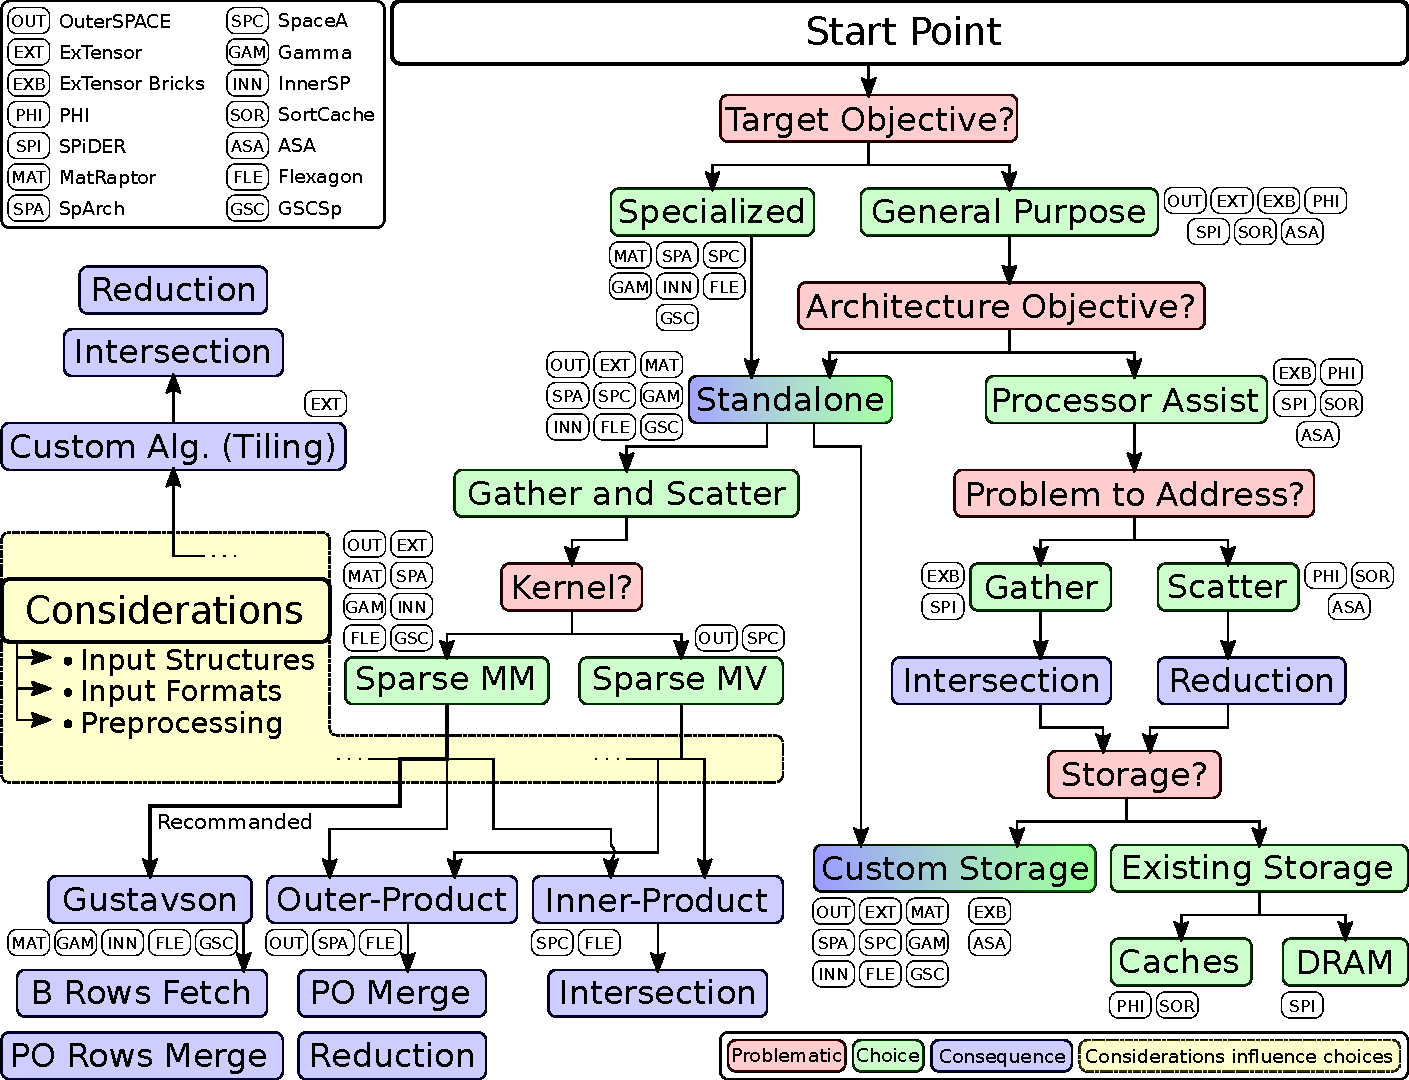
\includegraphics[width=\linewidth]{Chapter_SoA/Figures/PDF/Taxonomy.pdf}
    \caption{Flow Diagram for Architecture Selection}
    \label{fig:soa:taxonomy}
\end{figure}

There is no single "best overall" accelerator. A designer must consider the required performance, the available area and the class of problems to be addressed. In Figure~\ref{fig:soa:taxonomy} we present a flow diagram which can guide a designer towards an architecture based on their requirements. Starting from the top-right of the figure, the designer must first decide between a \emph{specialized accelerator} for a specific kernel or a \emph{general purpose accelerator}. The former is preferable if performance must be maximized, requiring a \emph{standalone} accelerator addressing both \emph{gather} and \emph{scatter} (\emph{e.g.} MatRaptor, SpArch, Gamma and InnerSP).

A \emph{general purpose accelerator} can either take the form of a highly configurable \emph{standalone} block (\emph{e.g.} OuterSPACE and ExTensor) or a \emph{processor assist} that boosts performance for a specific task. With a \emph{processor assist} (rightmost branch in the figure), the processor still performs important parts of the kernel, typically the multiplications, but off-loads the \emph{scatter} or \emph{gather} tasks to the accelerator, as these are the tasks which are the bottleneck with a traditional cache hierarchy. For example, for an \algo{IP} algorithm, the difficult part of the \emph{gather} task is performing the \emph{intersection} (e.g. the ExTensor bricks and SPiDRE).  Conversely, with \algo{OP} or \algo{Gust}, the challenge with the \emph{scatter} is to efficiently perform \emph{reductions} (e.g. PHI, SortCache and ASA). Finally, the designer must decide whether the storage is done by reusing existing memory resources (\emph{e.g.} PHI, SPiDRE and SortCache) or through custom caches/memories.

Going back to the case of a \emph{standalone} accelerator, the algorithms differ according to the supported kernels. For sparse MV, the accelerators studied here have opted for an \algo{OP} algorithm. For sparse MM, the designers of three of the five highest performing accelerators have chosen \algo{Gust} algorithm, as this algorithm provides a good trade-off, simplifying the \emph{gather} by reusing input $B$-rows and the row-by-row generation of the output, simplifying the \emph{scatter} aspect. The fact that the outputs are generated row-by-row, facilitates parallel implementations. \algo{Gust} works well with \emph{(UOP, CP)}, providing consistent input and output formats. Beyond the basic algorithm, \emph{tiling} approaches, as proposed by ExTensor, can be explored.

Orthogonal to previous choices, other design considerations are important. First, the starting point needs to be defined: some accelerators require software to perform \emph{tiling} (\emph{e.g.} ExTensor) or to rearrange the rows to improve performance (\emph{e.g.} Gamma). The cost of such preprocessing can be high, and is usually only justified if the same matrix is reused multiple times.

% %%%%%%%%%%%%%%%%%%%%%%%%%%%%%%%%%%%%%%%%%%%%%%%%%%%%%%%%%%%%%%%%%%%%%
% Conclusion 
% %%%%%%%%%%%%%%%%%%%%%%%%%%%%%%%%%%%%%%%%%%%%%%%%%%%%%%%%%%%%%%%%%%%%%

\section{Conclusion}
\label{sec:soa:conclusions}

% % Messages à passer
% \begin{itemize}
% \item Emerging field, increased activity
% \item Comparison of the SoA
% \item Memory hierarchy - not just a processing problem
% \item Gustavson
% \item Meta-data can be used to optimize caching strategies
% \item Innovative re-Use (re-purpose) of existing HW memory resources --> these accelerators can be integrated into existing memory systems
% \item Perhaps the key challenging is a highly parallelized reduction/merger
% \item None of the existing accelerators has focused on specific matrix structures
% \end{itemize}

The size of the datasets considered in computational physics, machine learning and graph analytics is continuing to grow and over the last six years, we note the emergence of many hardware accelerators designed to improve upon the performance of CPUs and GPUs. In this paper, we have presented the most important designs and established a comparison, while highlighting the underlying hardware challenges associated with sparse multiplication kernels.

As we have seen, with this class of problem, the challenge is to efficiently use the memory system despite the dereferencing required to access the \emph{metadata} associated with the \emph{sparse data formats}. Depending on the selected MM algorithm, the major challenge is either with the \emph{gather} and \emph{intersection} or with the \emph{scatter} updates. We have identified that accelerators based on \emph{Gustavson's} algorithm achieve a trade-off, where, on the \emph{gather} side, a limited number of $B$-rows need to be accessed, and on the output side, the result is generated row-by-row, simplifying the \emph{scatter} updates. The best \emph{Gustavson} accelerators have implemented further optimizations such as smart cache eviction strategies where the victim is selected by looking ahead at the $A$-indices. Several of the smaller \emph{processor assist} accelerators reuse existing cache memories and simply modify the behaviour of the control logic (directories, tags, eviction policies) to optimize the operation for sparse matrices. On the other hand, the highest performance accelerators propose dedicated, massively parallel \emph{reduction}/\emph{mergers}, to maximize parallelism.

Given the number and diversity of existing designs, it is clear that further hardware optimizations and improvements are possible. As stated earlier, there may never be a single "best" sparse accelerator, but rather designs that are best suited to specific classes of problems. We believe that the structure of the matrices is critical in terms of the sizing of caches and other resources, and that in the coming years, new accelerators will be increasingly tailored based on the structure of the matrices for specific classes of problems.

%%%%%%%%%%%%%%%%%

\clearpage
%%%%%%%%%%%%%%%%%%%%%%%%%%%%%%%%%%%%%%%%%%%%%%%%%%%%%%%%%%%%%%%%%%%%%%%%%
% CHAPTER SpDCache
%%%%%%%%%%%%%%%%%%%%%%%%%%%%%%%%%%%%%%%%%%%%%%%%%%%%%%%%%%%%%%%%%%%%%%%%%

\chapter[SpDCache]{SpDCache}
\label{cha:spdc}

\minitoc

% \input{}



%%%%%%%%%%%%%
%%from ASAP

%%red cache and op spmv behavior
% Performing a \emph{reduction} in hardware requires a \emph{READ} from memory,
% followed by an accumulation and a \emph{WRITE} back. This operation is denoted
% $\mathit{RED}(key, value)$~\cite{Srikanth2021_SortCache} with the \emph{key} being
% the position in the output vector $c$.
% In Fig.~\ref{fig:GC_cache_WB}, we show three cases that occur in a generic data cache when a
% \emph{reduction} is performed. If the vector entry ($c_{key}$) 
% \emph{hits} in the cache, the \emph{update} is performed by the processor
% with no external memory access.
% When there is a \emph{miss}, the operation is blocked until 
% the \emph{READ} from main memory completes. Potentially, the \emph{miss} will also 
% trigger an \emph{eviction}, which exacerbates the blocking condition, because
% a cache-line must first be written back, before the \emph{READ} from main memory can 
% be performed. In scientific applications, the matrices are extremely
% large and only a small portion of the vector $c$ can reside in the cache, thus
% the \emph{miss+evict} case arises frequently.

% A \emph{reduction cache}, such as~\cite{Srikanth2021_SortCache} or~\cite{Mukkara2019_PHI},
% is a data-cache which accepts
% \emph{reduction} instructions (\emph{RED}) from the processor and performs accumulations locally (near-memory).
% In the case of a \emph{hit}, see Fig.~\ref{fig:red_based_cache}, the \emph{reduction}
% takes place in the cache. For a \emph{miss}, the cache allocates a new line
% with zeros, and simply inserts the value. In this case,
% the cache-line is inconsistent with main memory. Only when the line needs to be evicted,
% is a \emph{READ} performed. In the cache, the values in the line are accumulated with the main memory data, and the result
% is written back. As seen in the figure, a \emph{reduction cache} reduces the number
% of main memory accesses in the case of a \emph{miss}. At the end of the algorithm, the cache
% must be flushed.

% \begin{figure}[htbp]
%     \centering
%     \begin{subfigure}[t]{0.506493506\linewidth} %39/77 (39/73)
%         \centering
%         
\includegraphics[width=\linewidth]{Figures/PDF/HardwareSpecs_RWtransactions_1.pdf}
%         \caption{Generic Cache (Write-Back)}
%         \label{fig:GC_cache_WB}
%     \end{subfigure}
%     \hfill
%     \begin{subfigure}[t]{0.441558442\linewidth} %34/77 (34/73)
%         \centering
%         
\includegraphics[width=\linewidth]{Figures/PDF/HardwareSpecs_RWtransactions_2.pdf}
%         \caption{Reduction Cache}
%         \label{fig:red_based_cache}
%     \end{subfigure}
%     \caption{\emph{READ} and \emph{WRITE} Transactions of a \emph{Reduction} Operation in Generic and \emph{Reduction} Caches}
%     \label{fig:RWtransactions}
% \end{figure}

% A widely used \emph{sparse format} to compress the non-zero elements in the matrix $A$ is \emph{CSC} (\emph{Compressed Sparse Column})~\cite{Saad2003_COO_CSR_DIA_ELL},
% where $A$ is a sparse matrix of dimensions $(M, N)$ with a number of non-zero elements $\mathit{NNZ}$. 
% It consists of three tables ($\mathit{VAL}$, $\mathit{IDX}$, $\mathit{PTR}$) used to store non-zero values, row indices and column positions.
% When performing an \algo{OP} SpMV ($A.b = c$) with this format (Algorithm~\ref{alg:spmv_with_red}),
% we see that a \emph{RED} is needed to accumulate the output vector $c$ (line~6). Moreover, $A$ is read sequentially 
% while $c$ is updated ``randomly''.
% In fact, the \emph{key} is determined via an indirection with an access to $\mathit{IDX}$.

% \begin{algorithm}[htbp]
%     \def\_{\!\!\!\!\!\!}
%     \caption{\emph{Outer-Product} SpMV -- Single Threaded}\label{alg:spmv_with_red}
%     \For(\Comment*[f]{\_ loop \_ over \_ columns \_ of \_ A \_}){$n \in \ldb 0, N-1 \rdb$}{
%         $\mathit{currPos}, \mathit{nextPos} \gets \mathit{PTR}_n, \mathit{PTR}_{n+1}$\;
%         \For{$pos \in \ldb \mathit{currPos}, \mathit{nextPos}-1 \rdb$}{
%             $key \gets \mathit{IDX}_{pos}$\Comment*[r]{\_ row \_ index \_}
%             $val \gets \mathit{VAL}_{pos} \times b_n$\Comment*[r]{\_ val \_ = \_ A\textsubscript{key,n} \_ $\times$ \_ b\textsubscript{n} \_}
%             $\mathit{RED}(key, val)$\Comment*[r]{\_ c\textsubscript{key} \_ += \_ val \_}
%         }
%     }
% \end{algorithm}

% In memory, $A$ is stored as three dense tables, but conceptually, as we perform
% the \algo{OP} multiplication, the matrix is traversed from top to bottom, then left to right. A row
% in the matrix corresponds to a \emph{key}, or equivalently, a position in the output vector $c$. In
% Fig.~\ref{fig:spmv_on_matrix}, we show an example of a sparse matrix with a few non-zero values
% (\ding{192} - \ding{197}). 
% As we traverse the matrix, we first perform a \emph{reduction} for the value on row $\mathit{key}_{10}$,
% then on row $\mathit{key}_{20}$ and then $\mathit{key}_{30}$. Each of these results in a 
% \emph{RED} on $c$. As we continue, we then \emph{hit} another
% value \ding{196} on the row $\mathit{key}_{10}$ which must be \emph{reduced} with an existing entry \ding{192}
% (as shown on the left of Fig.~\ref{fig:spmv_on_matrix}, \emph{Conceptual View}).

% \begin{figure}[htbp]
%     \centering
%     
\includegraphics[width=1\linewidth]{Figures/PDF/HardwareSpecs_SpMVonMatrix.pdf}
%     \caption{Traversal of Non-Zero Elements of Input Matrix for \algo{OP} SpMV (left) and Impact on Cache (right)}
%     \label{fig:spmv_on_matrix}
% \end{figure}

% Let us consider how $c$ is stored in a two-way set-associative cache with 32B lines.
% We assume that all the \emph{keys} map to $\mathit{set}_1$.
% When \ding{192} is updated, there is a \emph{miss} and $\mathit{line}_1$ is allocated for $\mathit{key}_{10}$.
% Similarly with \ding{193}, $\mathit{line}_2$ is allocated for $\mathit{key}_{20}$.
% When $\mathit{key}_{30}$ comes along, an \emph{eviction} must be performed. We assume $\mathit{line}_1$, holding $\mathit{key}_{10}$,
% is evicted. We then come to \ding{195} which has $\mathit{key}_{13}$, adjacent in memory to $\mathit{key}_{10}$,
% and thus stored in the same line. This line must be brought back to process \mbox{\ding{195} - \ding{197}}.

% This example illustrates how a conventional cache can be inefficient.
% First, we note the line holding $\mathit{key}_{10}$ was evicted, although it
% was frequently accessed after \ding{192}. This \emph{eviction} was triggered by $\mathit{key}_{30}$, which was only accessed once. 
% Furthermore, for $\mathit{key}_{20}$ and $\mathit{key}_{30}$, a full line was loaded, only to 
% modify a single entry. A ``smarter'' cache would have maintained the line with $\mathit{key}_{10}$ 
% to avoid an unnecessary main memory access. Furthermore, this ``smarter'' cache would not have
% allocated full lines for $\mathit{key}_{20}$ and $\mathit{key}_{30}$ to only modify a single word.
% In the following sections, we explain how SpDCache achieves these ``smart'' behavior.

%%archi SpDC
% As shown in Fig.~\ref{fig:cache_partition}, SpDCache is divided into three regions\footnote{SpDCache could be implemented as a mode of a generic cache.}. The first, \emph{GRC} (\emph{Generic Region Cache}), is 
% for all memory transactions unrelated to the output vector $c$, including reads of $A$ and $b$.
% It is a classic, set-associative cache and not our focus, but is required for the processor to operate normally.
% The other two regions, called \emph{IBRC} and \emph{OBRT}, are able to perform \emph{reductions} on $c$.
% The \emph{IBRC} works as a line-wise, set-associative \emph{reduction cache} to hold high density data in the \emph{IBR}.
% The difference with the \emph{GRC} is that it
% is able to perform \emph{reductions} and it is dedicated to the \emph{banded} region, so that spurious accesses do not provoke undesired \emph{evictions}.
% Finally, the \emph{OBRT} works as an element-wise, fully-associative table whose role is to handle sparse regions (\emph{OBR}).

% \vspace{-5mm}
% \begin{figure}[htbp]
%     \centering
%     \begin{minipage}[b]{0.58\linewidth}
%         \begin{figure}[H]
%     		\centering
%     		
\includegraphics[width=\linewidth]{Figures/PDF/HardwareSpecs_MatrixAndDataCachePartition.pdf}
%     		\caption{Data-Cache Partitioning into Regions (GRC, IBRC, OBRT)}
%     		\label{fig:cache_partition}
%     	\end{figure}
%     \end{minipage}
%     \hfill
%     \begin{minipage}[b]{0.38\linewidth}
%     	\begin{figure}[H]
%     		\centering
%     		
\includegraphics[width=\linewidth]{Figures/PDF/HardwareSpecs_GlobalViewArchi_Simplified.pdf}
%     		\caption{Simplified View of the Memory Hierarchy with SpDCache}
%     		\label{fig:global_view_archi}
%     	\end{figure}
%     \end{minipage}
% \end{figure}

% Fig.~\ref{fig:global_view_archi} shows a simplified view of a memory hierarchy with SpDCache. The \emph{Processor Interface} (\emph{PI}) takes
% \emph{reduction} operations, \emph{RED(key, value, region)}, from the processor and dispatches them to the \emph{IBRC} and \emph{OBRT}, depending on the \emph{region} argument.
% The \emph{IBRC} communicates with the memory hierarchy using \emph{READ} and \emph{WRITE} transactions over entire cache-lines, to propagate the local \emph{updates}
% to the downstream memory.
% As \emph{OBRT} \emph{updates} are for isolated elements, it does not make sense to bring a full line into the L1 to modify a 
% single word. 
% The \emph{OBRT} thus propagates \emph{updates} by issuing atomic Read-Modify-Write transactions (\emph{RMWs}), which must be processed remotely and 
% close to the main memory. 
% Existing protocols such as \mbox{AXI-4}~\cite{ARM2023_AXI} already support atomic transactions for certain operations (logical, integer add, min, max) and
% these would need to be extended to include floating point addition.
% The \emph{RMWs} from the \emph{OBRT} are temporarily buffered in a small queue (\emph{RMWQ}), to avoid congestion.

% SpDCache is driven by three key design principles.
% First, we ensure a given \emph{key} is in only one region, to avoid coherency problems.
% Second, the \emph{IBRC} is given priority over the \emph{OBRT}, to enable coalescing.
% Third, we avoid bringing a full line from memory to the L1 to simply update a few entries.

% \begin{figure}[htbp]
%     \centering
%     
\includegraphics[width=1\linewidth]{Figures/PDF/HardwareSpecs_SpDC_behavior.pdf}
%     \caption{Internal Operation of SpDCache with Examples} % Internal Operation of SpDCache
%     \label{fig:spdc_archi}
% \end{figure}

% In Fig.~\ref{fig:spdc_archi}, we describe the operation of SpDCache, 
% via a series of scenarios, each shown in a different color.
% When a new \emph{reduction} \emph{RED(key, value, region)} is received from the processor, 
% we test for a \emph{hit} in the \emph{IBRC}, regardless of the \emph{region} argument.
% If it \emph{hits}, the value (case \addr{0b} -- \textit{turquoise}) can be accumulated in 
% the corresponding line of the \emph{IBRC}. We give this priority to the \emph{IBRC} as
% part of the mechanism to avoid duplication.

% If there is a \emph{miss} in the \emph{IBRC}, then the target region is 
% determined based on the \emph{region} argument of the \emph{RED} transaction.
% If it is \emph{IBR}, then it
% is necessarily a \emph{miss} case, and the value (\addr{02} -- \textit{orange}) must be inserted into a free cache-line of 
% the \emph{IBRC}. When we allocate this line, we ensure that it does not create
% a duplication of existing entries in the \emph{OBRT}. If there is duplication, as in
% our example, these entries (\addr{00}, \addr{02}, \addr{06}) are deleted from
% the \emph{OBRT} and merged into the newly allocated line ($set_1, line_1$).

% If the target region is the \emph{OBR}, then the \emph{reduction} (\addr{3d} -- \textit{purple})
% is processed in the \emph{OBRT}, either allocating a new entry (\emph{miss} case) or accumulating with 
% an existing entry (\emph{hit} case).

% Now, we describe the \emph{eviction} scenarios. In the \emph{IBRC}, the line to evict is selected
% ($set_2, line_2$ -- \textit{pink}), a \emph{READ} to main memory is performed, the values from
% the evicted line are accumulated and a \emph{WRITE} to main memory is issued.
% If the evicted line only has a few
% non-zero elements, it is a special case. To avoid bringing a full line
% from main memory, the non-zero values (\addr{a1} and \addr{a5} -- \textit{blue}) are 
% converted to atomic \emph{RMWs} and pushed onto the \emph{RMWQ}.

% The width of the \emph{band} ($W_B$), must be selected so that one column of the \emph{band}
% remains blocked in the \emph{IBRC}, otherwise, this region of the cache is
% always thrashing. This is our approach to selecting $W_B$ and it is independent of the matrix.

% In the \emph{OBRT}, an \emph{eviction} simply consists of moving the element from the table to the 
% \emph{RMWQ} (\addr{8c} -- \textit{brown}).
% \emph{OBRT} \emph{evictions} are issued in advance when the table is nearly full.
% The \emph{RMWQ} issues atomic \emph{RMWs} when it is not empty (\addr{56} -- \textit{dark green}).


%%experimental results
% We modeled the behavior of SpDCache (based on the flowchart in Fig.~\ref{fig:spdc_archi}) using a transaction-level model in Python, for a single-core, 
% single-thread system executing a \algo{OP} SpMV kernel (Algorithm~\ref{alg:spmv_with_red}).
% We do not model timing, as the order of the memory accesses determines the behavior of the cache
% (\emph{hits}, \emph{misses}, \emph{evictions}), which depends only on the SpMV algorithm.
% The model checks the final numerical result and reports the main memory traffic associated with 
% the \emph{updates} to the output vector (\emph{Output Memory Traffic}), where 
% we count the bytes transferred (64B for each \emph{READ} and \emph{WRITE}, and 8B per atomic \emph{RMW}, 
% with our configuration). For each \emph{WRITE} transaction, it tracks how many words in the line 
% were actually used (\emph{Evicted Cache Line Utilization}) and it tracks how many 
% words in the cache held useful data (\emph{Cache Memory Utilization}). We consider a word 
% in the cache to be useful if it is updated or inserted by the processor.
% Our goal is to validate the principle of SpDCache using real application matrices 
% from SuiteSparse Matrix Collection~\cite{Kolodziej2019_SuiteSparse}.

% As baselines, we implemented a fully generic cache (GC) that handle \emph{READs} and \emph{WRITEs} for both 
% inputs ($A$, $b$) and output ($c$), following the data movements shown in Fig.~\ref{fig:GC_cache_WB}, and 
% a simple \emph{reduction cache} (RedC) that processes \emph{RED} transactions in a dedicated region 
% using the flow shown in Fig.~\ref{fig:red_based_cache}.
% In the RedC, 25\% of the memory is allocated for the inputs and the other 75\% for \emph{REDs} on $c$.
% In SpDCache (SpDC), 25\% is allocated for the \emph{GRC}, 50\% for the \emph{IBRC}
% and 25\% for the \emph{OBRT}.
% All three caches use a \emph{random} eviction policy and have a total data storage of 32~kiB, and we do not account
% for the \emph{TAG} storage. The set associative regions have 4~ways 
% and 64B cache lines (8 \emph{double} words per line).

% We simulated 48 matrices that have been used by the state-of-the-art accelerators~\cite{Pal2018_OuterSPACE, Hegde2019_ExTensor, Srivastava2020_MatRaptor, Baek2021_InnerSP, Zhang2021_Gamma, Srikanth2021_SortCache, Zhang2022_ASA}. 
% In Table~\ref{tab:results}, we report the results for a representative subset; the
% gains with the full set are similar. Most, but not all, of the matrices have a dense \emph{band}
% and even some matrices without an obvious \emph{band} benefit from the blocking 
% effect in the \emph{IBRC}.

% As expected, the simple \emph{reduction cache} (RedC) decreases the
% main memory traffic to 39.2\% of the GC baseline. 
% SpDCache has significantly better performance than the RedC, reducing the traffic to 12.3\%.

% The benefits of SpDCache can be partly explained by the improved
% utilization of the cache-lines. On average, a line evicted from the
% \emph{IBRC} has 7.46 modified words, compared to 3.69 and 3.91 with
% the baselines. This improved utilization is the result of blocking the dense region in the \emph{IBRC}.

% We need to consider an additional metric, the percentage of traffic sent as atomic \emph{RMW} transactions (\textit{\%~ATO}).
% If this value is too high, it means we have simply shifted the workload to the lower level caches, which inherently have limited compute capability.
% This is the case for the \emph{msc10848} matrix where 70.9\% of the traffic is atomic \emph{RMWs}, where a very large fraction of the non-zero values are outside the \emph{band}.
% Conversely, the \emph{raefsky3} matrix is an example were no atomic \emph{RMWs} are used, as the region outside the \emph{band} was empty. In this case, 25\% of the available memory was unused.

% To facilitate comparison with other accelerators, we simulated the set of matrices used by OuterSPACE~\cite{Pal2018_OuterSPACE}, 
% a commonly used baseline (not shown in Table~\ref{tab:results}). On these matrices, SpDCache's memory traffic is $8.8\times$ lower than \emph{GC}.

% \begin{table*}[t]
%     \def\colorR{Red}
%     \caption{Decrease in Memory Traffic and Improvement in Cache Utilization from Python Simulation}
%     \label{tab:results}
%     \centering
%     \begin{tabular}{|c|c|| *{2}{>{\centering\arraybackslash}m{1.0cm}|}| >{\centering\arraybackslash}m{1.0cm}|| *{3}{>{\centering\arraybackslash}m{1.0cm}|}| *{3}{>{\centering\arraybackslash}m{1.0cm}|}}
%         %\hline
%         \hhline{|--||---||---||---|}
%         \multirow{3}{*}{\textbf{Matrix}} & \multirow{3}{*}{\textbf{NNZ} / \textbf{M}} & \multicolumn{3}{c||}{\textbf{Output Memory Traffic}} & \multicolumn{3}{c||}{\textbf{Evicted Cache Line Utilization}} & \multicolumn{3}{c|}{\textbf{Cache Memory Utilization} (\%)} \\
%         %\cline{3-11}
%         %\hhline{|~~|--||-||---||---|}
%         & & RedC & \multicolumn{2}{c||}{SpDC} & GC & RedC & SpDC & GC & RedC & SpDC \\
%         & & \textit{\%/GC} & \textit{\%/GC} & \textit{\% ATO} & \textit{Avg} & \textit{Avg} & \textit{Avg} & \textit{Avg} & \textit{Avg} & \textit{Avg} \\
%         %\hline \hline
%         \hhline{:==::=:=::=::=:=:=::=:=:=:}
%         \textit{consph} & $6.0m$ / $83k$ & $23.5$ & $14.6$ & $27.9$ & $6.17$ & $6.60$ & $7.87$ & $48.5$ & $89.7$ & $96.8$ \\
%         \textit{roadNet-CA} & $5.5m$ / $2.0m$ & $61.9$ & $25.3$ & $14.0$ & $4.31$ & $3.75$ & $7.64$ & $39.6$ & $50.1$ & $83.0$ \\
%         \textit{pdb1HYS} & $4.3m$ / $36k$ & $11.9$ & $8.1$ & $22.5$ & $5.89$ & $6.97$ & $7.89$ & $48.7$ & $86.8$ & $95.3$ \\
%         \textit{offshore} & $4.2m$ / $0.3m$ & $77.9$ & $8.4$ & $43.4$ & $1.96$ & $1.87$ & $7.23$ & $31.7$ & $27.1$ & $80.1$ \\
%         \textit{webbase-1M} & $3.1m$ / $1.0m$ & $71.5$ & $34.9$ & $37.0$ & $5.77$ & $5.40$ & $8.00$ & $42.4$ & $65.7$ & $90.4$ \\
%         \textit{ramage02} & $2.9m$ / $17k$ & $9.5$ & $4.6$ & $44.1$ & $5.21$ & $6.42$ & $7.85$ & $47.7$ & $81.9$ & $94.1$ \\
%         \textit{filter3D} & $2.7m$ / $0.1m$ & $50.9$ & $10.6$ & $35.3$ & $2.72$ & $3.28$ & $7.14$ & $35.9$ & $50.4$ & $86.0$ \\
%         \textit{2cubes\_sphere} & $1.6m$ / $0.1m$ & $58.0$ & $8.7$ & $33.5$ & $2.29$ & $2.24$ & $7.49$ & $36.5$ & $31.2$ & $79.7$ \\
%         \textit{mac\_econ\_fwd500} & $1.3m$ / $0.2m$ & $28.3$ & $22.9$ & $4.6$ & $4.40$ & $6.04$ & $7.62$ & $42.4$ & $70.7$ & $73.6$ \\
%         \textit{scircuit} & $1.0m$ / $0.2m$ & $71.0$ & $22.6$ & $35.4$ & $3.95$ & $3.60$ & $7.94$ & $40.2$ & $46.7$ & $91.0$ \\
%         \textit{wiki-Vote} & $0.1m$ / $8.3k$ & $62.1$ & $5.1$ & $29.5$ & $1.74$ & $1.81$ & $5.68$ & $29.4$ & $25.0$ & $62.2$ \\
%         \hhline{|--||--||-||---||---|}
%         \multicolumn{2}{|c||}{\textbf{Geometric Mean}} & $\mathbf{39.2}$ & \hspace{1mm} $\mathbf{12.3}$ \!\!\! \hyperlink{fn0}{$^\mathrm{a}$} & $\mathbf{25.9}$ & $\mathbf{3.69}$ & $\mathbf{3.91}$ & \hspace{1mm} $\mathbf{7.46}$ \!\!\! \hyperlink{fn1}{$^\mathrm{b}$} & $\mathbf{39.7}$ & $\mathbf{51.9}$ & \hspace{1mm} $\mathbf{84.1}$ \!\!\! \hyperlink{fn2}{$^\mathrm{c}$} \\
%         %\hline \hline
%         \hhline{:==::=:=::=::=:=:=::=:=:=:}
%         \textit{raefsky3} & $1.5m$ / $21k$ & $19.7$ & \textcolor{\colorR}{$26.3$} & \textcolor{\colorR}{$0.0$} & $7.98$ & $8.00$ & $8.00$ & $49.5$ & $95.4$ & \textcolor{\colorR}{$65.0$} \\
%         \textit{msc10848} & $1.2m$ / $11k$ & $35.9$ & $14.4$ & \textcolor{\colorR}{$70.9$} & $4.96$ & $5.73$ & $7.86$ & $47.5$ & $72.0$ & $92.6$ \\
%         %\hline
%         \hhline{|--||--||-||---||---|}
%         \multicolumn{11}{l}{\hypertarget{fn0}{$^\mathrm{a}$Decrease by $8.1\times$ compared to GC.} \quad \hypertarget{fn1}{$^\mathrm{b}$Increase by $2.0\times$ compared to GC.} \quad \hypertarget{fn2}{$^\mathrm{c}$Increase by $2.1\times$ compared to GC.}}
%     \end{tabular}
%     \vspace{-1mm}
% \end{table*}

%%conclu
% We have presented the concept of SpDCache, a \emph{reduction cache} that has optimized storage and compute techniques for the sparser and denser regions of \emph{banded} matrices.
% This approach does not reduce the number of compute operations, however, it significantly decreases memory traffic ($8.1\times$).
% These benefits can be attributed to three techniques: (1) blocking the dense part of the \emph{band} in the \emph{IBRC}, (2) using fine-grained storage in the \emph{OBRT}
% and (3) off-loading the \emph{reductions} for isolated elements to the downstream caches, to prevent local \emph{evictions} and reduce traffic.

% Exploiting the coarse-grain structure of matrices is key to design hardware optimized for sparse matrix kernels.
% In future work, we plan to also take advantage of local fine-grain density in the \emph{OBR}, to further reduce memory traffic, and evaluate speedup on a clock-accurate model.

\clearpage
%%%%%%%%%%%%%%%%%%%%%%%%%%%%%%%%%%%%%%%%%%%%%%%%%%%%%%%%%%%%%%%%%%%%%%%%%
% CHAPTER Theory
%%%%%%%%%%%%%%%%%%%%%%%%%%%%%%%%%%%%%%%%%%%%%%%%%%%%%%%%%%%%%%%%%%%%%%%%%

\chapter[Theory]{Theory}
\label{cha:theory}

\minitoc

% \input{}



%%%%%%%%%%%%
%%from HPCA
%%background
% In Figure~\ref{fig:banded_mat_def}, we illustrate a banded, square matrix of dimension $M$.
% We define $w_B$ as the width of the banded region, or \textit{bandwidth}, as shown in \textit{red} in the figure. 
% Sometimes it is easier to refer to the half-\textit{bandwidth}, $w_{hB}$, which respects the relation $w_B = 2w_\mathit{hB} - 1$.
% The average density in the band and out of the band is defined as $d_\mathit{IB}$ and $d_\mathit{OB}$, respectively.
% In a \textit{perfectly banded} matrix, there are no elements outside the band, thus $d_\mathit{OB} = 0$.

% \begin{figure}[htbp]
%     \centering
%     % \begin{minipage}[b]{0.33980583\linewidth} % 17.5/51.5
%     %     \begin{figure}[H]
%     %         \centering
%     %         
\includegraphics[width=\linewidth]{Figures/PDF/MatrixDef.pdf}
%     %         \caption{Banded Matrix Definition}
%     %         \label{fig:banded_mat_def}
%     %     \end{figure} 
%     % \end{minipage}
%     % \hfill
%     \begin{minipage}[b]{0.63106796\linewidth} % 32.5/51.5
%         \begin{figure}[H]
%             \centering
%             
\includegraphics[width=\linewidth]{Figures/PDF/MatrixSpMVRep.pdf}
%             \caption{Visual Representation of \algo{OP} SpMV Computation}
%             \label{fig:op_spmv_rep}
%         \end{figure}
%     \end{minipage}
% \end{figure}

% Sparse matrices are used in many kernels, such as sparse matrix-vector (SpMV) and sparse matrix-matrix multiplication (SpMM).
% These kernels can be implemented with several algorithms.
% Many works~\cite{Isaac2024_SoA, Mukkara2019_PHI, Pal2018_OuterSPACE} have shown that the \textit{Outer-Product} (\algo{OP}) algorithm has the potential to enhance performance, if computed with an adapted hardware architecture.
% For sparse kernels, the performance is almost always limited by the indirect accesses induced by the sparse formats.
% The indirections are ``random'' and have limited spatial and temporal locality, limiting the effectiveness of traditional caches.
% For \algo{OP} algorithms, these indirect accesses occur when updating the output vector, which are referred to as ``scatter updates''.

% Many software solutions focus on improving performance, using conventional compute hardware including CPUs and GPUs~\cite{MOHAMMED_2022_SPARSE}, but since the performance limitation comes from the memory system, custom hardware solutions are required.
% PHI~\cite{Mukkara2019_PHI}, SortCache~\cite{Srikanth2021_SortCache} and ASA~\cite{Zhang2022_ASA} modify the cache hierarchy for an existing processor to support scatter updates.
% This type of accelerator, called a \textit{reduction cache}, has the advantage of being general purpose, offering a performance improvement to any algorithm requiring ``random'' scatter updates.
% The focus of this paper is a new \textit{reduction cache} architecture, which exploits the coarse- and fine-grained structure of the matrix, to improve performance, unlike previous solutions.

% Our analysis is focussed on the \algo{OP} SpMV kernel, \mbox{$A \times b = c$}, shown in Algorithm~\ref{alg:op_spmv}.
% The solution is equally applicable to SpMM kernels with \textit{Gustavson}'s algorithm~\cite{Gustavson1978_GustAlgo} or other ``push''-type graph algorithms.
% \algo{OP} SpMV is the sparse version of matrix-vector multiplication that simply consists in $c_{i} \acc A_{i,j} \times b_j$ for all $0 \leqslant i, j \leqslant M-1 \in \mathbb{N}$, computed column-first.
% It behaves differently than the row-first, \textit{Inner-Product} version.
% The matrix $A$ is sparse and is usually stored in the CSC sparse format (\textit{Compressed Sparse Column})~\cite{Saad2003_CSR}, which consists in three 1D-tables: $\mathit{val}$ of size $nnz$, containing all the non-zero elements, sorted by column; $\mathit{idx}$ of size $nnz$, containing the row-index of every non-zero element; $\mathit{ptr}$ of size $M+1$, containing the position of each column in tables $\mathit{val}$ and $\mathit{idx}$.
% The vectors $b$ and $c$ are dense (one table each).

% \begin{algorithm}[htbp]
%     \caption{\algo{OP} SpMV: $A \times b = c$}\label{alg:op_spmv}
%     \For(\Comment*[f]{Column-first}){$j \in \ldb0, M-1\rdb$}{
%         \For{$\mathit{pos} \in \ldb\mathit{ptr}_j, \mathit{ptr}_{j+1}-1\rdb$}{
%             $\mathit{i} \gets \mathit{idx}_{\mathit{pos}}$\;
%             $c_{\mathit{i}} \gets c_{\mathit{i}} + \mathit{val}_{\mathit{pos}} \times b_j$\Comment*[r]{RED}
%         }
%     }
% \end{algorithm}

% When computing an \algo{OP} SpMV, the matrix is read column by column, left to right, traversing the columns top to bottom, shown in Figure~\ref{fig:op_spmv_rep}.
% Each non-zero element of row $i$ (horizontally) will eventually be accumulated into the output vector $c$ at index $i$.
% In our representation, we show the output vector $c$ at the right of the matrix.
% Since the traversal of the matrix $A$ is column-wise, each element of $c$ is progressively updated.

% With the \algo{OP} algorithm and CSC format, reads to $A$ and $b$ occur on consecutive addresses, both being read once.
% Caches benefit from the spatial locality of these accesses and effectively mask the external memory latency.
% Because $A$ is sparse, the reads and writes to $c$ do not necessarily occur on consecutive addresses.
% This is due to indirections when accessing $c$ via the $\mathit{idx}$ table of $A$: $c_{idx_{pos}}$.
% The obstacle to high performance are these ``random'' scatter updates to $c$ and in the next sections, we study the cache behavior when updating $c$.

% In \algo{OP} SpMV, the accesses that occur to $c$ consist of a read of $c_i$, a modification (accumulation with partial product $\mathit{val}_\mathit{pos} \times b_j$) and a write to update $c_i$, which is referred to as a \textit{reduction} (line 4 of Algorithm~\ref{alg:op_spmv}).
% For other ``push''-type algorithms, the modify operation may change (e.g. logical OR...) but the read-modify-write pattern is the same.
% \textit{Reduction caches} are specialized data-caches that can natively perform \textit{reductions}.
% Indeed, instead of considering the \textit{reduction} as two separate memory transactions, it becomes a single memory transaction, $\mathit{RED}(\mathit{address}, \mathit{value})$.
% This new operation can be implemented as a single, ``fire-and-forget'' instruction, meaning the processor does not need to wait for a response, unlike a load instruction.
% The value of the \textit{reduction} is then simply stored or accumulated in the cache, and merged to main memory when the cache-line must be evicted.
% This ``write-back''-like policy removes unnecessary memory traffic and masks memory read response latency.
% The \textit{reduction cache} computes accumulations internally, using a local arithmetical unit, a form of near-memory computing.
% Existing accelerators such as PHI, SortCache and ASA are based on a \textit{reduction cache}.
% In addition, they each have their own unique approach to manage the spatial irregularity of the \textit{reductions}.
% Indeed, a simple \textit{reduction cache} is not sufficient to manage these ``random'' accesses, as we will show in Section~\ref{sec:theory}.

% In our analysis of \textit{reduction caches}, we use a set-associative configuration, with $8$ byte elements which we consider as the basic memory unit.
% $s_C$ is the size of the cache, in elements.
% The cache is divided into \textit{sets}, ways and cache-lines, of size $S$, $W$ and $l$, respectively.
% Thus, $s_C = S \times W \times l$ elements.

% Our focus is on banded matrices, thus for each non-zero element, we must determine if it is in or out of the band.
% This could be done in the inner-loop of the algorithm (lines 4-7 of Algorithm~\ref{alg:op_spmv}), by checking $|j - pos| \leqslant w_\mathit{hB}$, but this adds many instructions in the critical inner-loop.
% To avoid this overhead, we propose a dedicated sparse format called BaCSC (\textit{Banded CSC}) that adds the in- or out-of-band information in the $\mathit{ptr}$ table.
% In the standard CSC $\mathit{ptr}$ table, two consecutive entries of indices $k$ and $k+1$ indicate the position in the $\mathit{idx}$ and $\mathit{val}$ tables of the first non-zero element of column $k$ and $k+1$.
% In the BaCSC $\mathit{ptr}$ table, we add two entries, to indicate the position in the $\mathit{idx}$ and $\mathit{val}$ tables of the first and the last non-zero element of the in-band region of column $k$.
% This extended $\mathit{ptr}$ table has a size of $3M+1$, but enables the location of the band to be determined in the outer-loop, reducing the instructions in the inner-loop.

%%model
% Many previous works~\cite{Zhang2021_Gamma, Isaac2024_SpDCache, Srikanth2021_SortCache, Isaac2024_SoA} observed the critical role played by the structure of the matrix in the efficiency of sparse hardware accelerators.
% To go beyond simply observing the behavior of a specific accelerator processing a given matrix, a model of the matrix and the cache is required.
% We present a hybrid probabilistic/fast simulation model for a \textit{reduction cache}, processing \algo{OP} SpMV, which predicts the volume of memory traffic issued by the L1 cache, starting from a matrix density distribution and a cache configuration.

% The model represents the non-zero density both in the matrix and in the cache, with cache-line granularity.
% Using these coarse grain densities, a fast simulation of the \algo{OP} SpMV is performed.
% The state of the cache can be predicted at each step of the simulation.
% By counting the evictions, we evaluate the update memory traffic.
% We can thus predict the total number of memory accesses for different types of matrices and quickly explore different \textit{reduction cache} configurations.

% We do not consider the sequential accesses to the input matrix $A$ and vector $b$ in our model.
% Indeed, the matrix tables $\mathit{val}$, $\mathit{idx}$ and $\mathit{ptr}$, and the vector $b$ are each read once, giving a total memory traffic of $2\mathit{nnz} + (M+1) + M$ elements.
% The latency for these sequential accesses can be masked with a linear prefetcher~\cite{Smith1982_Prefetcher}, and a small generic cache.

% Our model uses the cache configuration parameters $S$, $W$ and $l$.
% Although our model is not limited to banded matrices, they are the focus of this work.
% The matrix density distribution thus takes on two different values, either $d_\mathit{IB}$ in the band, or $d_\mathit{OB}$ outside of the band, as shown in Figure~\ref{fig:banded_mat_def}.

% We normalize the memory traffic by dividing the number of elements that are read or written by the number of non-zero elements ($nnz$) in the matrix, so we can compare performance between matrices of different sizes and densities.
% Indeed, we can interpret the normalized memory traffic, $\mathit{normMT}$, as the number of elements transferred from/to memory per non-zero matrix element.
% If the memory traffic remains constant while the matrix density increases, we expect $\mathit{normMT}$ to decrease.

% % %%%%%%%%%%%%%%%%%%%%%%%%%%%%%%%%%%%%%%%%%%%%%%%%%%%%%%%%%%%%%%%%%%%%%
% \subsection{Operation of the Analytical Model}
% \label{sec:model}

% \paragraph{Matrix Representation}
% The square matrix is of dimension $M$, as represented in Figure~\ref{fig:model:matrix_cache_rep}.
% Its rows and columns are indexed by $0 \leqslant i, j \leqslant M-1 \in \mathbb{N}$.
% Each column is split into vertical-strips of size $l$, where $l$ is the cache-line size.
% Indeed a vertical-strip is a portion of a column $j$ of size $l$, from row-indices $i$ to $i+l-1$, as illustrated by the \textit{red} rectangle within the matrix in the figure.
% Within a column, vertical-strips are indexed by $k \in \ldb0, M_l-1\rdb$~\footnote{We use $\ldb a, b\rdb$ for the integer intervals, and $[a, b]$ for real intervals.}, with $M_l = \left\lceil\frac{M}{l}\right\rceil$, and $k = \left\lceil\frac{i}{l}\right\rceil$.

% The matrix is thus represented as a static, dense two dimensional table, $\mathit{MDT}$ (\textit{Matrix Density Table}), of size $(M_l, M)$ that contains the density in $[0, 1]$ of each vertical-strip.
% We assume that the distribution of the non-zero elements within a vertical-strip is uniform, as assumed in related work~\cite{Temam1992_Model} where the authors only studied a directly-mapped generic cache for an \textit{Inner-Product} SpMV kernel, for the case of \textit{perfectly banded} matrices.

% \begin{figure}[htbp]
%     \centering
%     \includegraphics[width=\linewidth]{Figures/PDF/CModel_matrix&cache_rep.pdf}
%     \caption{Input Matrix and Cache Representation of Vector $c$}
%     \label{fig:model:matrix_cache_rep}
% \end{figure}

% \paragraph{Cache Representation}
% Still in Figure~\ref{fig:model:matrix_cache_rep}, the cache is represented as a single column, which maps directly to the output vector $c$.
% This ``column-representation'' of the cache is partitioned into cache-lines, corresponding directly to the vertical-strips of a given column of the matrix, as shown by the horizontal \textit{light red} rectangle.
% A cache-line $k \in \ldb0, M_l-1\rdb$ is stored in a unique \textit{set} $s \in \ldb0,S-1\rdb$ of the cache such that $s = k \% S$.
% Unlike the matrix representation which is static, the cache representation is continuously updated as the model evaluates \algo{OP} SpMV.

% Of course, the real cache-size is not necessarily equal to the output vector size.
% Thus, at a given time, the number of valid (non-empty) cache-lines contained in the cache representation must not exceed the actual cache-size.
% Specifically, we ensure the number of valid cache-lines in a \textit{set} does not exceed the number of ways $W$.
% In the example in Figure~\ref{fig:model:matrix_cache_rep}, the actual cache is holding four valid cache-lines, which are the only valid cache-lines present in the cache representation.

% To count the number of valid cache-lines, we further distinguish them from empty ones.
% For this reason, we set the cache-line densities to be either zero (the cache-line is empty), or the density is in the range $\left[\frac{1}{l}, 1\right]$ (the cache-line is valid).
% A valid cache-line has a density between $\frac{1}{l}$ and $1$, corresponding to the probabilistic number of non-zero elements.

% The state of the cache is thus represented with the dynamic table $\mathit{DCDT}$ (\textit{Disjoint Cache Density Table}), of dimension $M_l$ that contains the disjoint-density in $\{0\} \cup \left[\frac{1}{l}, 1\right]$ of each cache-line, at a given iteration.
% Initially, all cache-lines are set to zero density, since the cache is considered empty.

% \paragraph{Iterative Process}
% In the fast simulation phase, the analytical model~\cite{FRIEDENTHAL2012_AnalyticalModel} iterates over the vertical-strips in the matrix, following the dense traversal of the \algo{OP} algorithm, as described in Section~\ref{sec:background} and shown with \textit{red} arrows in Figure~\ref{fig:model:matrix_cache_rep}.
% In a given iteration (column $j$, vertical-strip $\kappa$), we use the matrix density of the current vertical-strip, $\mathit{MDT}_{\kappa,j}$, and the current state of $\mathit{DCDT}$ to determine if an eviction occurs, and update it for the next iteration, if necessary.

% \paragraph{Disjoint-Density of the Current Vertical-Strip}
% The density of the current vertical-strip in the matrix has to be disjointed at each iteration, to determine whether the strip is empty or not, as done for the cache-lines.
% We define the vertical-strip disjoint-density as $d_\mathit{lM}(\kappa) \in \{0\} \cup [\frac{1}{l}, 1]$.
% \begin{itemize}
%     \item When $\mathit{MDT}_{\kappa,j} = 0$, the vertical-strip in the matrix is empty, thus, $d_\mathit{lM}(\kappa) = 0$.
%     \item When $0 < \mathit{MDT}_{\kappa,j} < \frac{1}{l}$, the vertical-strip can have either $0$ or $1$ non-zero elements.
%             To resolve this, we maintain a running counter of the accumulated $\mathit{MDT}_{\kappa,j}$ values, and when this counter exceeds $\frac{1}{l}$, the current vertical-strip is considered non-empty, so we set $d_\mathit{lM}(\kappa) = \frac{1}{l}$.
%             If the counter is below this threshold, $d_\mathit{lM}(\kappa) = 0$.
%             %To avoid undesired aliasing artifacts, we add a small random variation to this threshold.
%     \item When $\mathit{MDT}_{\kappa,j} \geqslant \frac{1}{l}$, the vertical-strip has one or several non-zero elements.
%           Thus, $d_\mathit{lM}(\kappa) = \mathit{MDT}_{\kappa,j}$.
% \end{itemize}

% With this definition, we can distinguish empty ($d_\mathit{lM}(\kappa) = 0$) and non-empty ($d_\mathit{lM}(\kappa) \ne 0$) vertical-strips.

% \paragraph{Eviction Processing}
% With the above definitions, we can determine if a miss occurs at the current iteration.
% A miss occurs when the cache-line $\kappa$ is not valid and the vertical-strip is not empty.
% Recall that in a \textit{reduction cache}, a miss without eviction results in the allocation of a free cache-line, initially filled with zeros, and produces no memory traffic.
% We define \mbox{$\mathit{miss}(\kappa) = (\mathit{DCDT}_\kappa = 0) \; and \; (d_\mathit{lM}(\kappa) \ne 0)$}, a boolean indicating whether a miss occurs in the current iteration.

% When allocating a free cache-line, it is necessary to ensure that the number of valid cache-lines in the \textit{set} \mbox{$s = \kappa \% S \in \ldb0,S-1\rdb$} does not exceed $W$.
% The new allocation may thus trigger an eviction.
% Stated formally, $\mathit{nnzcl}_\kappa$ is the count of the cache-lines $k$ from the \textit{set} $s$ that verify $\mathit{DCDT}_k \ne 0$.
% We define \mbox{$\mathit{evict}(\kappa) = \mathit{miss}_\kappa \; and \; (\mathit{nnzcl}_\kappa = W)$}, a boolean indicating whether an eviction occurs in the current iteration.

% In the case of an eviction, for the probabilistic model, we use a \textit{random} eviction policy to select a valid cache-line in the \textit{set} $s$ (when $\mathit{DCDT}_k \ne 0$).
% The index of the evicted cache-line is $e \in \ldb0, M_l-1\rdb$.

% \paragraph{Cache Update}
% The last step is to update $\mathit{DCDT}$ before proceeding to the next iteration.
% (1) If a cache-line is evicted, we must account for the memory traffic and reset the victim line $e$.
% (2) The density of the current cache-line $\kappa$ may increase if there is a hit or if it is newly allocated.

% (1) In the case of an eviction ($\mathit{evict}(\kappa)$ is true), we reset the victim cache-line ($e$) by setting $\mathit{DCDT}_e = 0$.

% (2) We update the density of the cache-line $\kappa$.
% In the case of a miss ($\mathit{DCDT}_\kappa = 0$), the cache-line density is set to the disjoint-density of the matrix vertical-strip $\kappa$.
% In the case of a hit, the cache-line and the vertical-strip densities are merged: $\mathit{DCDT}_\kappa \gets \mathit{DCDT}_\kappa + (1 - \mathit{DCDT}_\kappa) \times d_\mathit{lM}(\kappa)$.
% The updated cache-line density is either $0$ or greater than $\frac{1}{l}$, thus respecting the constraint that the cache-line is either empty or valid.

% \paragraph{Final Iteration}
% Starting with an initially empty cache, we run all $M \times M_l$ iterations and count the total number of evictions ($\mathit{nbEvict}$).
% After the last iteration, we account for the memory transactions required to flush the cache ($\mathit{nbFlush}$), writing the valid cache-lines to memory, by counting lines where $\mathit{DCDT}_k \ne 0$, for $k \in \ldb0, M_l-1\rdb$.
% % The number of memory accesses to flush the cache ($\mathit{nbFlush}$) will never exceed \mbox{$S \times W$}, the size of the cache.

% In a \textit{reduction cache}, evictions and flushes result in a line-wise memory read, a modification, and a line-wise memory write.
% The update memory traffic is $2 l (\mathit{nbEvict} + \mathit{nbFlush})$ elements, and $\mathit{normMT}$ is this amount divided by $nnz$.

%%theory
% We now study the \textit{reduction cache} behavior when computing \algo{OP} SpMV, starting with the simple case of \textit{perfectly banded} matrices with varying \textit{bandwidths}.
% We then use the analytical model to analyse the \textit{reduction cache} behavior, varying the out-of-band density and the cache-size.
% We show the benefit of storing the in- and out-of-band of the matrix in separate regions of the cache, to achieve low memory traffic.

% % %%%%%%%%%%%%%%%%%%%%%%%%%%%%%%%%%%%%%%%%%%%%%%%%%%%%%%%%%%%%%%%%%%%%%
% \subsection{Behavior of a Perfect-Band in a Cache}
% \label{sec:perfectband_vs_cache}

% \begin{figure}[htbp]
%     \centering
%     \begin{subfigure}{0.49\linewidth}
%         \centering
%         
\includegraphics[width=\linewidth]{Figures/PDF/PBrotationCase1_0.pdf}
%         \caption{Column iteration $j$}
%         \label{fig:in_band_rotation_00}
%     \end{subfigure}
%     \hfill
%     \begin{subfigure}{0.49\linewidth}
%         \centering
%         
\includegraphics[width=\linewidth]{Figures/PDF/PBrotationCase1_1.pdf}
%         \caption{Column iteration $j+1$}
%         \label{fig:in_band_rotation_01}
%     \end{subfigure}
%     \caption{Example of the Eviction Rotation in a Perfect Band when the Cache is Undersized ($s_C < w_B + l - 1$)}
%     \label{fig:in_band_rotation_case1}
% \end{figure}

% \begin{figure}[htbp]
%     \centering
%     \begin{subfigure}{0.49\linewidth}
%         \centering
%         
\includegraphics[width=\linewidth]{Figures/PDF/PBrotationCase2_0.pdf}
%         \caption{Column iteration $j$}
%         \label{fig:in_band_rotation_10}
%     \end{subfigure}
%     \hfill
%     \begin{subfigure}{0.49\linewidth}
%         \centering
%         
\includegraphics[width=\linewidth]{Figures/PDF/PBrotationCase2_1.pdf}
%         \caption{Column iteration $j+1$}
%         \label{fig:in_band_rotation_11}
%     \end{subfigure}
%     \caption{Example of the Eviction Rotation in a Perfect Band when the Cache is `Properly' Sized ($s_C = w_B + l - 1$)}
%     \label{fig:in_band_rotation_case2}
% \end{figure}

% We now show why the \textit{reduction cache} must be `properly' dimensioned with respect to the \textit{bandwidth} of a \textit{perfectly banded} matrix, in order to avoid unnecessary evictions when processing an \algo{OP} SpMV kernel.
% Indeed, if the cache is too small compared to the band, evictions occur before the column iteration is over, leading to poor data-reuse for the next iteration.
% To achieve high data-reuse, we show that the cache-size ($s_C$) and the \textit{bandwidth} ($w_B$) must respect the relationship given in Equation~\ref{eq:in_band_cond}.

% \begin{equation}
%     s_C \geqslant w_B + l - 1
%     \label{eq:in_band_cond}
% \end{equation}

% We consider two examples with a cache having four cache-lines ($L_1$ to $L_4$) with $l = 6$.
% In Figure~\ref{fig:in_band_rotation_case1}, we illustrate the case when the cache is too small ($s_C < w_B + 5$).
% In Figure~\ref{fig:in_band_rotation_00}, we see the state of the cache after iterating up to column $j$.
% Then, in Figure~\ref{fig:in_band_rotation_01}, we see the state after processing the next column, $j+1$.
% The cache-line $L_1$ (\textit{orange}) is evicted, and allocated to new elements at the bottom of the band, below the \textit{yellow} area.
% In this case, there are still elements of the band above the \textit{green} area, whose corresponding cache-line has, unfortunately, been evicted.
% Thus, on iteration $j+2$, cache-line $L_1$ must be fetched again and this pattern continues creating \textit{thrashing}.

% In Figure~\ref{fig:in_band_rotation_case2}, we illustrate the case when the cache is `properly' sized ($s_C \geqslant w_B + 5$).
% As in the previous example, Figures~\ref{fig:in_band_rotation_10} and~\ref{fig:in_band_rotation_11} show the state of the cache at iterations $j$ and $j+1$, respectively.
% This time, the cache-line $L_1$ is evicted only when all elements of the band in the \textit{orange} region have been processed.
% Indeed, the eviction of cache-line $L_1$ occurs just in time so that it can be allocated to the new region at the bottom of the band, below the \textit{yellow} area.
% In this way, when processing columns, the cache-lines do a rotation where the top one is evicted and allocated at the bottom, with one eviction occurring after the processing of every $l$ columns.

% If the cache-size is larger than required by Equation~\ref{eq:in_band_cond}, the rotations are the same, the eviction-rate is the same, but each cache-line accumulates more elements, increasing the hit-rate.
% To produce this perfect cache rotation, we assume an LRU eviction policy and dense vertical-strips, although, even with a \textit{random} policy, the general pattern still holds.

% This analysis shows that, with a ``properly-sized'' \textit{reduction cache}, a \textit{perfectly banded} matrix provokes no unnecessary evictions and the cache-lines are fully utilized.
% Many real matrices are banded, but are rarely \textit{perfectly banded}, and next, we study the impact of non-zero elements out of the band.

% % %%%%%%%%%%%%%%%%%%%%%%%%%%%%%%%%%%%%%%%%%%%%%%%%%%%%%%%%%%%%%%%%%%%%%
% \subsection{Impact of Out-Of-Band Density on Memory Traffic}
% \label{sec:graph1}

% We now apply the analytical model of Section~\ref{sec:redcache_model} to analyse the performance of a \textit{reduction cache} for banded matrices, processing an \algo{OP} SpMV kernel ($A \times b = c$).
% We consider banded matrices of dimension $M = 1000$, with a half-band of size $w_\mathit{hB} = 125$ and an in-band density $d_\mathit{IB} = 1$.
% We analyse a 4-way set-associative cache ($W = 4$) with a cache-line size of $l = 8$ elements, with a \textit{random} eviction policy.
% The size of the cache varies from $S = 1$ to $S = 32$ \textit{sets}.
% When the cache-size reaches $S = 32$, the cache can hold the full output vector: $S \times W \times l \geqslant M$.
% In Figure~\ref{fig:theory_traffic_vs_d_ob}, we plot the normalized memory traffic, $\mathit{normMT}$, for the output vector $c$, depending on the out-of-band density $d_\mathit{OB}$, for varying cache-sizes.

% \begin{figure}[htbp]
%     \centering
%     
\includegraphics[width=\linewidth]{Figures/PDF/graph1_25.07.31.pdf}
%     \caption{Normalized Output Memory Traffic Depending on the Out-of-Band Density for Several Cache-Sizes}
%     \label{fig:theory_traffic_vs_d_ob}
% \end{figure}

% On the right of the graph, we notice that $\mathit{normMT}$ reaches a peak when the out-of-band density equals \mbox{$\frac{1}{l} = 0.125$}.
% Indeed, when there is at least one non-zero element per cache-line, the behavior of the cache approaches that seen for a dense matrix.
% As the density increases further, the traffic remains constant, thus $\mathit{normMT}$ drops, as seen in the graph in Figure~\ref{fig:theory_traffic_vs_d_ob}

% For the plot corresponding to $S = 32$, the cache is large enough to store the entire output vector $c$, thus, there are no evictions and $\mathit{normMT}$ is constant, corresponding to the flush traffic at the end.
% This plot gives the lower bound of memory traffic for the output vector $c$.

% The first takeaway of this graph is that variations in $d_\mathit{OB}$ heavily impact $\mathit{normMT}$.
% Isolated non-zero elements outside the band trigger misses and evictions of cache-lines corresponding to the banded region.
% Furthermore, when a cache-line is allocated for an isolated out-of-band element, most of the cache-line remains empty.
% In this case, instead of the efficient rotating pattern described in Section~\ref{sec:perfectband_vs_cache}, the cache is \textit{thrashing} with low utilisation.
% Regardless of the cache-size, the lower the out-of-band density, the lower $\mathit{normMT}$, as seen by the plots that tend downward toward the left of the graph.
% Avoiding the perturbations induced by the out-of-band elements would enable the cache to achieve minimal memory traffic, as with a \textit{perfectly banded} matrix.

% Not surprisingly, at the left of the graph, $\mathit{normMT}$ varies depending on the cache-size.
% This is due to the relative size of the band and the cache.
% Indeed, if the matrix \textit{bandwidth} is large compared to the cache-size, processing one column of the band will generate many evictions.
% To avoid evictions in the band, the relationship given by Equation~\ref{eq:in_band_cond} in Section~\ref{sec:perfectband_vs_cache} must be fulfilled.
% Indeed, for this example, for $S \geqslant 8$, this relationship holds and the corresponding plots have significantly lower $\mathit{normMT}$.
% Conversely, the first three plots ($S = 1$ to $4$) do not respect this condition, explaining their high $\mathit{normMT}$.
% Thus, the second takeaway from this graph is that, given a cache memory size, there is an ideal \textit{bandwidth} that generates minimal $\mathit{normMT}$.
% Increasing the cache-size beyond this threshold only produces a minor reduction in memory traffic, since at the beginning of matrix traversal, the first eviction is deferred before reaching the steady state rotating pattern, as discuss in Section~\ref{sec:perfectband_vs_cache}.

% These observations lead us to divide the cache into two regions.
% One which is optimized for storing the band and the other which handles all the other elements.
% The in-band region of the cache can thus operate with maximal efficiency corresponding to the bottom-left of Figure~\ref{fig:theory_traffic_vs_d_ob}.
% In subsequent sections, we analyse the out-of-band traffic.

% % %%%%%%%%%%%%%%%%%%%%%%%%%%%%%%%%%%%%%%%%%%%%%%%%%%%%%%%%%%%%%%%%%%%%%
% \subsection{Design Analysis for Out-of-Band Region}
% \label{sec:graph2}

% For the type of large matrices under study, there are usually too many non-zero elements in the out-of-band region for them to be cached from one column to the next, thus making it impossible to achieve the rotating pattern described in Section~\ref{sec:perfectband_vs_cache}.
% Therefore, the size of the cache for the out-of-band is not as important as the choice of associativity and data granularity.
% To justify this affirmation, we use the analytical model from Section~\ref{sec:redcache_model} to analyse the performance of the \textit{reduction cache} when processing only the non-zero elements outside of the band.
% As we have already discussed the handling of the in-band region, we now consider only the out-of-band elements, which is equivalent to setting the in-band density to $d_\mathit{IB} = 0$.
% Using the same matrix parameters as in the previous section, we explore different choices of cache-line size ($l \in \{1, 8\}$ elements), associativity (set-associative or fully-associative), memory transaction type (\textit{R/W} or \textit{RMW}), and total cache-size ($s_C \in \{128, 256\}$ elements).
% Because the out-of-band data is highly sparse, we want to explore having an element-wise cache ($l = 1$) instead of the typical line-wise cache ($l = 8$).
% As this cache region can be relatively small, a fully-associative configuration ($S = 1$, $l = 1$) is reasonable in terms of hardware implementation, and this full associativity makes full use of the storage.
% Indeed, when dealing with sparse elements, it is wasteful to bring a full line into the cache to only modify one element and then evict it, which we denote as \textit{R/W}.
% Thus, we consider offloading the \textit{reduction} to a higher level cache, thus reducing unnecessary data transfers.
% We assume the higher level cache can support this operation which we denote as \textit{RMW}.
% Indeed, protocols such as AXI~\cite{ARM2023_AXI} support atomic transactions (AMOs), which could easily be extended for \textit{reduction} operations.

% To validate that the cache-size is of secondary importance, we consider two different sizes (\textit{solid} and \textit{dashed}).
% For a given cache-size, we adjust the number of ways ($W$), based on the associativity, to keep the cache-size constant.
% In Figure~\ref{fig:theory_OBtraffic_vs_d_OB}, we plot $\mathit{normMT}$ for the output vector, depending on $d_\mathit{OB}$, for varying cache configurations.

% \begin{figure}[htbp]
%     \centering
%     
\includegraphics[width=\linewidth]{Figures/PDF/graph3_25.07.31_modif.pdf}
%     \caption{Normalized Output Memory Traffic of the Out-of-Band, Depending on the Density for Several Cache-Sizes}
%     \label{fig:theory_OBtraffic_vs_d_OB}
% \end{figure}

% Let us start by considering a classic set-associative cache with a line-wise memory interface (\textit{solid blue}, \textit{dot}), where we see a dependence of $\mathit{normMT}$ on $d_\mathit{OB}$.
% On the right of the graph ($d_\mathit{OB} \geqslant \frac{1}{l}$), we observe the same behavior as in Section~\ref{sec:graph1}, where the cache behavior approaches that seen for a dense matrix, where the cache tends to \textit{thrash}.

% Looking at the plot for the fully-associative cache with a line-wise memory interface (\textit{solid green}, \textit{square}), we see that the normalized traffic is not impacted by the density of the out-of-band, as expected.
% With the fully-associative cache, $\mathit{normMT}$ is constant near $16$, as, on average, there are two line-wise transactions per non-zero element processed, one read to fill the line, one write to evict it.

% The \textit{red} plots (\textit{diamond}) correspond to a fully-associative cache with an element-wise memory interface, which can offload element-wise \textit{RMW} transactions.
% We see that this approach results in over an order magnitude reduction in $\mathit{normMT}$.
% First, we avoid transferring full cache-lines which are mostly empty, and we only send the \textit{RMW} in one direction (``fire-and-forget'').
% Indeed, $\mathit{normMT}$ is now reduced to below one transaction per non-zero element processed.
% The fact that this value is below one shows that this cache region does hit and reduce memory traffic.
% However, increasing the size of this cache does not significantly increase the hit-rate, as can be seen by the \textit{dashed} plots, which correspond to a $2\times$ larger cache, and which are not significantly lower than the corresponding \textit{solid} ones.

% To summarize, the characteristics needed for the out-of-band region are: (1) a fully-associative element-wise data-storage to avoid virtually empty cache-lines, (2) an element-wise memory interface to reduce memory traffic, and (3) a small storage region which is adequate.

% % %%%%%%%%%%%%%%%%%%%%%%%%%%%%%%%%%%%%%%%%%%%%%%%%%%%%%%%%%%%%%%%%%%%%%
% \subsection{Resulting Approach and Discussion}
% \label{sec:theory_conclu}

% In the previous sections, we analyzed the behavior of \textit{reduction caches} executing an \algo{OP} SpMV kernel with banded matrices.
% We evaluated the expected memory traffic using an analytical model, considering separately the in- and out-of-band regions.
% We identified the cache characteristics required for both regions, which are extremely different.
% We thus propose to divide the available cache memory into two dedicated regions: one for the in-band, and one for the out-of-band.

% To obtain the efficient rotating pattern for the in-band region, which is the key to massively reducing memory traffic, Equation~\ref{eq:in_band_cond} must be respected.
% In practice, this defines the size of the band that can be allocated to the in-band cache region.
% As we have seen, this cache region can operate efficiently with a set-associative line-wise configuration.

% For the out-of-band region, a fully-associative element-wise cache with an element-wise memory interface can significantly reduce the memory traffic.
% The size of this region is less critical, thus it is preferable to allocate the majority of the available storage to the in-band region.

% It is important to note that the analytical model that we have presented is based on the assumption of a uniform distribution of the non-zero elements.
% In practice, this is not always the case, and this non-uniformity can impact the cache behavior, as will be seen later in Section~\ref{sec:evaluation}.
% Indeed, if the non-zero elements are clumped, the cache-lines tend to be better filled, resulting in lower memory traffic.
% In other words, our uniform assumption leads to a pessimistic prediction of memory traffic.

\clearpage
%%%%%%%%%%%%%%%%%%%%%%%%%%%%%%%%%%%%%%%%%%%%%%%%%%%%%%%%%%%%%%%%%%%%%%%%%
% CHAPTER Microarchitecture
%%%%%%%%%%%%%%%%%%%%%%%%%%%%%%%%%%%%%%%%%%%%%%%%%%%%%%%%%%%%%%%%%%%%%%%%%

\chapter[Microarchitecture]{Microarchitecture and Evaluation}
\label{cha:arch}

\minitoc

% %%%%%%%%%%%%%%%%%%%%%%%%%%%%%%%%%%%%%%%%%%%%%%%%%%%%%%%%%%%%%%%%%%%%%
% %% Microarchitecture %%
% Introduction
% %%%%%%%%%%%%%%%%%%%%%%%%%%%%%%%%%%%%%%%%%%%%%%%%%%%%%%%%%%%%%%%%%%%%%

\section{Introduction}
\label{sec:arch:intro}

TODO

% we do a rtl implem of spdc for eval
% first, some details about the implem
% then, eval and new things around it (dcd)

\clearpage
% HPDcache
% %%%%%%%%%%%%%%%%%%%%%%%%%%%%%%%%%%%%%%%%%%%%%%%%%%%%%%%%%%%%%%%%%%%%%
% %% Microarchitecture %%
% Microarchitecture
% %%%%%%%%%%%%%%%%%%%%%%%%%%%%%%%%%%%%%%%%%%%%%%%%%%%%%%%%%%%%%%%%%%%%%



%% add RAM, nop, RTL, CAM



\section{Microarchitecture}
\label{sec:arch:microarch}

% In light of the above analysis, this section describes the architecture of a \gls{redC} capable of supporting multiple regions with distinct characteristics.
% We introduce OBaMMA, an \textit{\underline{O}uter-Product} \underline{Ba}nded \underline{M}atrix \underline{M}emory \underline{A}ccelerator.
\acrlong{spdc} features two primary capabilities.
First, as a \gls{redC}, it supports \textit{reduction} instructions, enabling the accumulation of data near-memory.
Second, it implements a region-based cache where regions have different data-granularity, levels of associativity and overall behavior.

% The OBaMMA cache has three regions:
% \begin{itemize}
%     \item The \acrshort{grc} (\textit{Generic Region Cache}) functions as a generic cache region.
%     It is useful for processing sequential memory accesses that occur during the computation of sparse kernels.
%     For example, in the \algo{OP} SpMV kernel, the \acrshort{grc} manages the sequential reads of matrix $A$ and vector $b$.
%     %
%     \item The \acrshort{drc} (\textit{Dense Region Cache}) operates as a line-wise set-associative \gls{redC}.
%     It exclusively processes \textit{reduction} instructions, in a write-back manner.
%     Data to be accumulated is held only in the cache.
%     Memory transactions, to synchronize main memory, are issued only on data \gls{eviction}.
%     This region is beneficial for matrix areas which exhibit high locality despite the apparent randomness of accesses, such as within the matrix band.
%     %
%     \item The \acrshort{srt} (\textit{Sparse Region Table}) functions as an element-wise fully-associative \gls{redC}.
%     Like the \acrshort{drc}, it processes \textit{reduction} instructions in a write-back manner but employs atomic element-wise memory transactions instead of the conventional line-wise read and write transactions.
%     This region is advantageous for matrix areas where elements are isolated, having minimal spatial locality, such as outside the band of a matrix.
% \end{itemize}

% This approach is similar to~\cite{Isaac2024_SpDCache} which already suggested that splitting a cache can reduce memory traffic, however, the analysis was empirical, based on a high-level Python model and the sizing of the regions was not addressed.
% Our work extends this by providing an analytical study that strengthens the concept and offers insights into region dimensioning.
% Additionally, OBaMMA includes a fully functional RTL implementation, enabling accurate performance and area evaluation, as presented in Section~\ref{sec:evaluation}.

\subsection{HPDcache: The RTL base generic cache}

\acrlong{spdc} is implemented into an L1 data cache for a CVA6 RISC-V core, building upon an existing open-source high-performance set-associative data cache known as HPDcache~\cite{Fuguet2023_HPDcache}.
In contrast to traditional data caches, HPDcache introduces new features, including buffering techniques for memory writes, set-associative storage to manage read \gls{miss} requests, and dynamic configurability of each cache-line to operate in either write-back or write-through modes.
It is designed for high performance, utilizing a three-stage pipeline to handle multiple instructions while minimizing stall potential through out-of-order cache execution.

An overview of \acrlong{spdc}'s microarchitecture is shown in Figure~\ref{fig:arch:microarch}, where \textit{black} and \textit{blue} components are originally from HPDcache.
The first stage (\textit{st0}) decodes instructions and issues reads to the cache directory and data RAMs (\textit{Dir} and \textit{Data}).
These reads require one cycle to respond.
In the second stage (\textit{st1}), the response indicates whether a \gls{hit} or \gls{miss} occurred and if an \gls{eviction} is necessary.
The instruction proceeds to the final stage (\textit{st2}) only if a \gls{miss} or \gls{eviction} must be processed.
At \textit{st0}, the instruction is not yet consumed.
Depending on the response and the availability of cache resources at \textit{st1}, a \textit{nop} (\textit{no operation}) may be inserted in the pipeline, and the instruction may be placed in a \textit{replay table}.
The instruction is then replayed with the highest priority once its dependencies are cleared.
If the instruction does not need to be replayed at \textit{st1}, it is consumed and processed.
This pipeline serves as the foundation for implementing \acrlong{spdc}'s \gls{reduction} operations.
% add infos on blocks such as UC, CMO..

HPDcache provides extensive static and dynamic configurability, making it a flexible foundation for further extensions.
To implement \acrlong{spdc} as well as a \gls{redC} baseline, we modified HPDcache to be highly configurable so that a single RTL implementation can produce multiple designs.
The RTL can be instantiated as a generic cache (the first baseline, \acrshort{gc}), as a \gls{redC} (the second baseline, \acrshort{redc}), or as \acrshort{spdc}, the solution presented in the previous chapters.

\subsection{RTL Implementation of SpDCache}

We configure the original HPDcache as a 4-way set-associative cache with 128 \glspl{set} and 64-byte cache-lines, resulting in a total cache size of 32~KiB.
We extend the three-stage pipeline to handle the new \gls{red} instruction.
Figure~\ref{fig:arch:microarch} provides an overview of \acrlong{spdc}'s microarchitecture, highlighting new blocks in \textit{red}, modified blocks in \textit{blue}, and untouched components in \textit{black}.
The overall architecture aligns with the design presented in Chapter~\ref{cha:spdc}, adapted here for hardware implementation.
Let us briefly describe the operation of the \acrshort{drc} under three scenarios: \glspl{hit}, \glspl{miss} with available cache-lines, and \glspl{miss} requiring \gls{eviction}.

\begin{figure}[htbp]
    \centering
    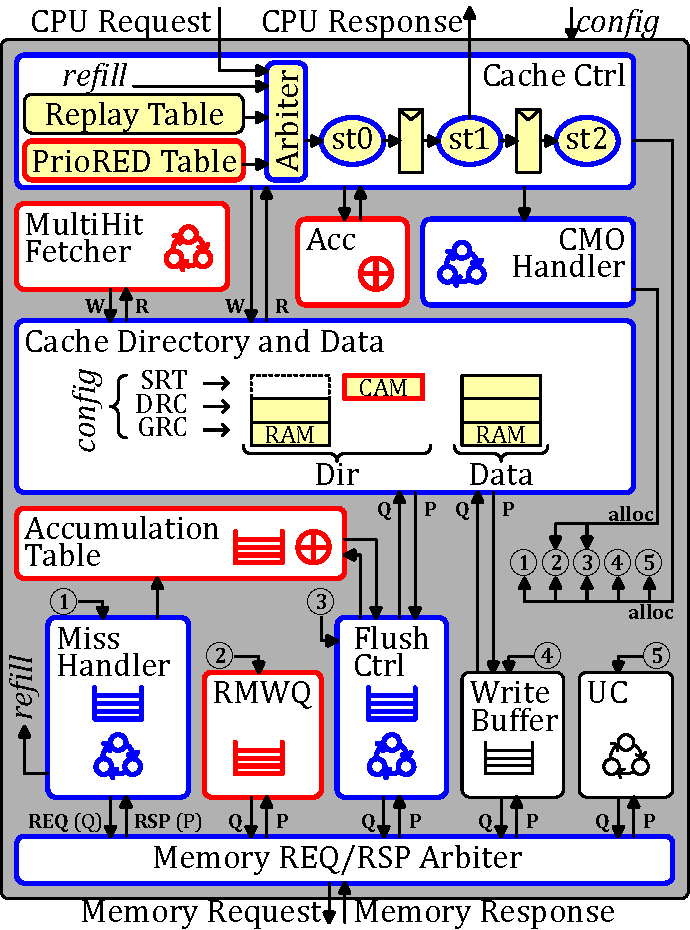
\includegraphics[width=0.7\linewidth]{Chapter_MicroArch/Figures/PDF/SpDC_MicroArchi.pdf}
    \caption{\acrlong{spdc} Microarchitecture, based on HPDcache \note{RMWQ}}
    \label{fig:arch:microarch}
\end{figure}

\textbf{In the case of a \gls{hit}}, the value of the \gls{red} instruction is accumulated with its corresponding value in the cache.
At \textit{st1}, the cache value, read in \textit{st0} from \textit{Data}, is accumulated with the \gls{red} value using a dedicated accumulator (\textit{Acc}).
The result is written back to \textit{Data} at \textit{st2}.

\textbf{In the case of a \gls{miss}}, if there is an available cache-line, the value of the \gls{red} instruction is simply stored in this free entry of the cache.
A free cache-line is selected at \textit{st1}, and at \textit{st2}, the \gls{red} value is written to \textit{Data} along with zeros to reset the selected cache-line.
A write to \textit{Dir} is also performed to change the state of the cache-line from free to valid.

\textbf{If a \gls{miss} occurs but no cache-line is free}, an \gls{eviction} must be processed before handling the \gls{red} instruction.
The \gls{red} instruction is placed in the \textit{PrioRED table} to be replayed with higher priority than the \textit{replay table}.
Meanwhile, at \textit{st2}, the \textit{miss handler}, \textit{flush controller}, and \textit{accumulation table} are allocated to process the \gls{eviction}.
The \gls{eviction} is a ``fire-and-forget'' operation, meaning the \gls{red} instruction only needs to wait for the entry in \textit{Data} to be freed, not for the entire \gls{eviction} to finish.
The \gls{eviction} process begins by fetching and resetting the chosen 64~B cache-line from \textit{Data}, which is done in one cycle by the \textit{flush controller}.
Simultaneously, the \textit{miss handler} issues a read to the main memory, which in our performance simulations, we assume will take 64 cycles to respond. \note{FIX}
The \textit{accumulation table} waits and temporarily stores both the old cache-line from the \textit{flush controller} and the 64~B response data from the \textit{miss handler}.
It then accumulates the cache-line with the data, word by word, and sends the 64~B results back to the main memory using the existing write interface.

With the changes described above, we have transformed \mbox{HPDcache} into a \gls{redC}.
To achieve multiple cache regions, we virtually separate the cache RAMs.
To maintain HPDcache's set-associative operation, we divide the cache memory along its \glspl{set}.
Thus, each region of the cache has the same structure as the overall cache but is smaller in size: each \gls{set} contains a fixed number (the number of ways) of 64-byte cache-lines, as depicted in Figure~\ref{fig:arch:set_redirection}.
Each region can map any possible address.
To ensure that every address matches a unique \gls{set} within each region, we allocate a power-of-two number of consecutive \glspl{set} to a region.
Considering the total number of \glspl{set} $S_T$ and our region $R$ mapping on $S_R < S_T$ of them, starting at the \gls{set} $s_\mathit{offset}$, if an address matches one of the \glspl{set} of this region, no action is required.
However, if the address matches a \gls{set} $s_\mathit{addr}$ outside the region, we need to map it to a unique \gls{set} in the region such that $s_\mathit{region} = (s_\mathit{addr} \% S_R) + s_\mathit{offset}$, as illustrated in Figure~\ref{fig:arch:set_redirection}.
The three regions \acrshort{grc}, \acrshort{drc}, and \acrshort{srt} are each defined by their number of \glspl{set} $S_R$ and their first \gls{set}, $s_\mathit{offset}$.
\acrlong{spdc} can thus be reconfigured to operate as a generic cache, a traditional \gls{redC} or a region-based \gls{redC} based on the needs of the application (\textit{config} in Figure~\ref{fig:arch:microarch}).

\begin{figure}[htbp]
    \centering
    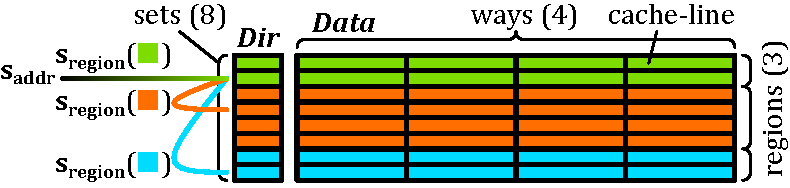
\includegraphics[width=\linewidth]{Chapter_MicroArch/Figures/PDF/Sets_redirection.pdf}
    \caption{Set Redirection Depending on the Region}
    \label{fig:arch:set_redirection}
\end{figure}

The \acrshort{srt} region requires additional adjustments to function as an element-wise fully-associative cache.
This region operates as if all the \glspl{set} were combined into a single \gls{set}, containing numerous elements.
Each element requires its own directory entry.
Therefore, we replace the \textit{Dir} RAMs of this region with a \textit{CAM} (\textit{Content-Addressable Memory}) containing the addresses of each valid element in the \acrshort{srt} region.
With the \textit{CAM}, we can check for a \gls{hit} across the entire region and retrieve the matching value stored in the \textit{Data} RAMs.
We also added a queue (\textit{RED AMO Queue}) \note{FIX} to manage the element-wise \gls{rmw} memory transactions.

To avoid address duplication between regions, the \textit{MultiHit fetcher} in Figure~\ref{fig:arch:microarch} manages coherency between the \acrshort{drc} and \acrshort{srt}, following the description in Chapter~\ref{cha:spdc}.
Since software selects the region, this can be necessary.
The \textit{MultiHit fetcher} performs two tasks.
First, given an address, it probes the \textit{CAM} for entries whose cache-line address matches.
If one or more matches are found, it records their positions locally and notifies the \textit{cache controller}.
Second, when activated, the \textit{MultiHit fetcher} gathers the corresponding elements from the \textit{Data} RAMs of the \acrshort{srt} and assembles them into a single 64~B line that will be written into the \acrshort{drc}.

%%%
We have added several custom instructions to the CVA6 RISC-V core~\cite{Waterman2016_RISCV_ISA}.
The primary addition is the \textit{reduction} instruction (\gls{red}), which takes an address and a value as arguments and expects no response.
This instruction is accompanied by a region instruction (\textit{REG}) that specifies in which region subsequent \textit{reductions} should be processed.
We have also added an instruction to flush the \textit{reduction} regions (\acrshort{drc} and \acrshort{srt}) of the cache, which is necessary at the end of the algorithm.
It is performed in the cache by the \textit{CMO handler}.
Finally, we have included an instruction to enable and disable the \textit{reduction} mode of \acrlong{spdc}.

\begin{figure}[htbp]
    \centering
    \begin{subfigure}{0.49\linewidth}
        \centering
        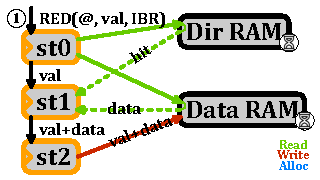
\includegraphics[width=\linewidth]{Chapter_MicroArch/Figures/PDF/SpDC_Pipeline_01.pdf}
        \caption{TODO}
        \label{fig:arch:pipeline_01}
    \end{subfigure}
    \hfill
    \begin{subfigure}{0.49\linewidth}
        \centering
        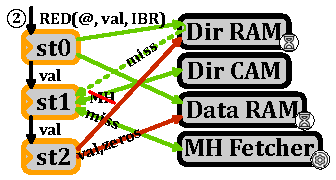
\includegraphics[width=\linewidth]{Chapter_MicroArch/Figures/PDF/SpDC_Pipeline_02.pdf}
        \caption{TODO}
        \label{fig:arch:pipeline_02}
    \end{subfigure}
    %
    \begin{subfigure}{0.49\linewidth}
        \centering
        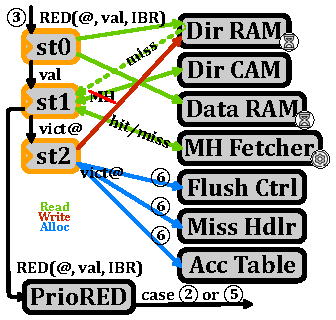
\includegraphics[width=\linewidth]{Chapter_MicroArch/Figures/PDF/SpDC_Pipeline_03.pdf}
        \caption{TODO}
        \label{fig:arch:pipeline_03}
    \end{subfigure}
    \hfill
    \begin{subfigure}{0.49\linewidth}
        \centering
        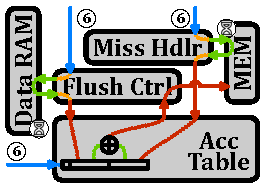
\includegraphics[width=0.8\linewidth]{Chapter_MicroArch/Figures/PDF/SpDC_Pipeline_06.pdf}
        \caption{TODO}
        \label{fig:arch:pipeline_06}
    \end{subfigure}
    %
    \begin{subfigure}{0.49\linewidth}
        \centering
        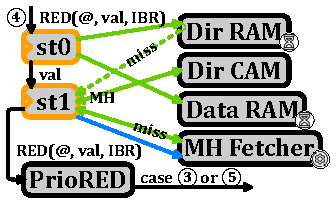
\includegraphics[width=\linewidth]{Chapter_MicroArch/Figures/PDF/SpDC_Pipeline_04.pdf}
        \caption{TODO}
        \label{fig:arch:pipeline_04}
    \end{subfigure}
    \hfill
    \begin{subfigure}{0.49\linewidth}
        \centering
        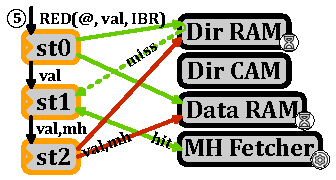
\includegraphics[width=\linewidth]{Chapter_MicroArch/Figures/PDF/SpDC_Pipeline_05.pdf}
        \caption{TODO}
        \label{fig:arch:pipeline_05}
    \end{subfigure}
    \caption{Pipeline Operation IBR}
    \label{fig:arch:pipeline_IBR}
\end{figure}

\begin{figure}[htbp]
    \centering
    \begin{subfigure}{0.49\linewidth} % [position][height][inner pos]{width}
        \centering
        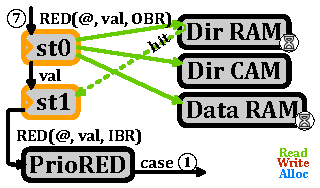
\includegraphics[width=\linewidth]{Chapter_MicroArch/Figures/PDF/SpDC_Pipeline_07.pdf}
        \caption{TODO}
        \label{fig:arch:pipeline_07}
    \end{subfigure}
    \hfill
    \begin{subfigure}{0.49\linewidth}
        \centering
        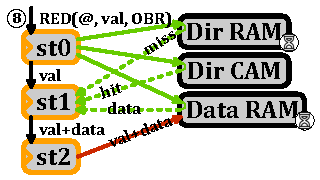
\includegraphics[width=\linewidth]{Chapter_MicroArch/Figures/PDF/SpDC_Pipeline_08.pdf}
        \caption{TODO}
        \label{fig:arch:pipeline_08}
    \end{subfigure}
    %
    \begin{subfigure}{0.49\linewidth}
        \centering
        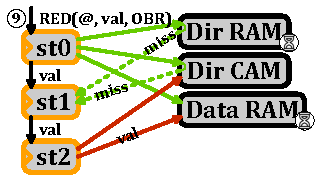
\includegraphics[width=\linewidth]{Chapter_MicroArch/Figures/PDF/SpDC_Pipeline_09.pdf}
        \caption{TODO}
        \label{fig:arch:pipeline_09}
    \end{subfigure}
    \hfill
    \begin{subfigure}{0.49\linewidth}
        \centering
        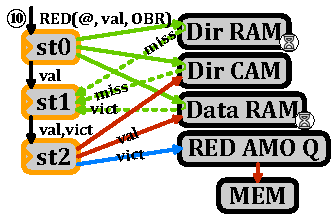
\includegraphics[width=\linewidth]{Chapter_MicroArch/Figures/PDF/SpDC_Pipeline_10.pdf}
        \caption{TODO \note{RMWQ}}
        \label{fig:arch:pipeline_10}
    \end{subfigure}
    \caption{Pipeline Operation OBR}
    \label{fig:arch:pipeline_OBR}
\end{figure}
% %%%%%%%%%%%%%%%%%%%%%%%%%%%%%%%%%%%%%%%%%%%%%%%%%%%%%%%%%%%%%%%%%%%%%
% %% Microarchitecture %%
% Introduction
% %%%%%%%%%%%%%%%%%%%%%%%%%%%%%%%%%%%%%%%%%%%%%%%%%%%%%%%%%%%%%%%%%%%%%

\section{Evaluation}
\label{sec:arch:eval}

TODO intro

% %%%%%%%%%%%%%%%%%%%%%%%%%%%%%%%%%%%%%%%%%%%%%%%%%%%%%%%%%%%%%%%%%%%%%
\subsection{Methodology for RTL Simulations}

The starting point is a CVA6~\cite{Zaruba2019_CVA6} RISC-V core with HPDcache~\cite{Fuguet2023_HPDcache} as an L1 data-cache with size 32~KiB ($S=128$, $W=4$, $l=8$ elements).
This serves as our baseline for performance comparison which we refer to as the \acrfull{gc}.
Next we evaluate a \gls{redC} which we derived from the HPDcache and configured to have two regions: a generic region with 16~KiB, and a \gls{reduction} region with 16~KiB whose behavior is the same as the \acrshort{drc} region of \acrlong{spdc}.
We refer to this design as \acrshort{redc}.
Finally, we evaluate \acrfull{spdc} with a reference configuration of: \acrshort{grc} = 8~KiB, \acrshort{drc} = 16~KiB, \acrshort{srt} = 8~KiB, which corresponds to the 25\%/50\%/25\% configuration selected in Chapter~\ref{cha:spdc}.
The configurations are summarized in Table~\ref{tab:arch:region_configs}.
All our simulations are performed using Siemens Questasim\texttrademark~2023.3 and the memory accesses beyond the L1 incur a fixed latency of 64 clock cycles.
We do not aim to evaluate a full system in this work, as our goal is to identify performance behavior using real matrices.
Thus, we use a single-core, single-cache-level environment.
The CVA6 core is not designed for high performance and can process at most one instruction per cycle.
We will discuss later how this limitation affects cache performance. \note{CHECK THIS AT THE END}
The fixed memory latency of 64 cycles is not realistic but provides a reasonable approximation of other memory levels' latencies and helps stabilize results for clearer interpretation.

% int64_t

% the hw constraint of the region sizes (could be fixed)

\begin{table}[htbp]
    \caption{Region Sizing of the Cache Configurations}
    \label{tab:arch:region_configs}
    \centering
    \begin{tblr}{
            width = {0.75\linewidth},
            colspec = {X[3cm,c] *{6}{X[c]}}, % rowspec
            rows = {m, font=\small},
            colsep = {1pt},
            row{1-Z} = {rowsep=2pt, black!2},
            column{2,4,6} = {r, rightsep=2pt},
            column{3,5,7} = {l, leftsep=2pt},
            row{1} = {c, font=\bfseries\small, black!5},
            cell{1}{2,4,6} = {c=2}{},
            hspan = {minimal},
            % hlines, vlines,
            % rulesep = {-1pt},
            hline{1,Z} = {2pt}, % Z for last
            hline{2} = {1pt},
            vline{2} = {1-Z}{0.5pt},
        }
        %
        Configurations & \acrshort{grc} & & \acrshort{drc} & & \acrshort{srt} & \\
        %
        \acrshort{gc}   & 100\% & ($S = 128$) & 0\%  & ($S = 0$)  & 0\%  & ($S = 0$)  \\
        \acrshort{redc} & 50\%  & ($S = 64$)  & 50\% & ($S = 64$) & 0\%  & ($S = 0$)  \\
        \acrshort{spdc} & 25\%  & ($S = 32$)  & 50\% & ($S = 64$) & 25\% & ($S = 32$)
    \end{tblr}
\end{table}

% %%%%%%%%%%%%%%%%%%%%%%%%%%%%%%%%%%%%%%%%%%%%%%%%%%%%%%%%%%%%%%%%%%%%%
\subsection{Sparse Formats Used for thr RTL Simulations}

By default, matrices are stored in \acrshort{csc} sparse format, and we use this format for most of our simulations.
However, in our evaluation, we try simulating \acrshort{spdc} with a specific format tailored for \acrshort{banded} matrices.
As shown in Figure~\ref{fig:arch:BaCSC}, compared to a \acrshort{csc}, we added extra information in the $ptr$ table to identify the beginning and end of the \gls{band}.
Indeed, three pointers instead of one are now needed per column, as shown with the example of column 2 in \textit{yellow}.
The column is split in one in-\gls{band} (IB) region in the middle and two out-of-\gls{band} (OB) regions around.
The $ptr$ table size thus becomes $3 \times M + 1$.
With this format, we can avoid the computational cost of identifying in which region non-zero elements are, while traversing the matrix, with the drawback of having to preprocess it.

\begin{figure}[htbp]
    \centering
    \includegraphics[width=\linewidth]{Chapter_MicroArch/Figures/PDF/SpFormats_BaCSC.pdf}
    \caption{Example of a Sparse Matrix in \acrshort{bacsc} Format}
    \label{fig:arch:BaCSC}
\end{figure}

\begin{highlight}{Conclusion}{Red}
    ..
\end{highlight}

% %%%%%%%%%%%%%%%%%%%%%%%%%%%%%%%%%%%%%%%%%%%%%%%%%%%%%%%%%%%%%%%%%%%%%
\subsection{Software Implementation of Outer-Product SpMV Kernel}

The code running on the CVA6 is written in generic C, compiled with \textit{gcc} 11.2.0 and -O3 optimization.
The \acrshort{red}-related instructions used in the \acrshort{op} \acrshort{spmv} kernel are manually inserted using \textit{asm} directives, as illustrated in Source Code~\ref{src:arch:op_spmv}.

\sourcecode{Chapter_MicroArch/Code/op_spmv.c}{C Code for the \acrshort{op} \acrshort{spmv} with \acrshort{red} Operations}{src:arch:op_spmv}{htbp}

The code shown is for \acrshort{spdc}.
Variants for other designs differ as follows: \acrshort{redc} omits region selection (line~15) and invokes \acrshort{reg} once before the loops with \acrshort{ibr} as the argument; \acrshort{gc} requires no \acrshort{reg} instruction and replaces \acrshort{red} with standard accumulation: $c[idx] \acc val$.

For \acrshort{spdc}, it is necessary to know the target region for each \acrshort{red} instruction based on the size of the \gls{band} (line~15).
The half-\gls{band} width $w_\mathit{hB}$ is derived from Chapter~\ref{cha:theory} (Equation~\ref{eq:theory:in_band_cond}) to ensure the in-\gls{band} region fits within the \acrshort{drc} independent of matrix structure.
In our reference configuration ($s_C(\mathit{DRC}) = 2048$, $l = 8$), $w_\mathit{hB} = 1021$.
Region selection follows Equation~\ref{eq:arch:reg_select} via an inline function, avoiding conditional branches within the inner-loop.

\begin{equation}
    \label{eq:arch:reg_select}
    \forall (i,j) \in \ldb 0, M-1 \rdb \times \ldb 0, N-1 \rdb, \; \mathit{region} = \left\{
    \begin{tabular}{ll}
        \acrshort{ibr} & if \; $|i-j| < w_\mathit{hB}$ \\
        \acrshort{obr} & else
    \end{tabular} \right.
\end{equation}

On-the-fly region computation introduces overhead in the critical inner-loop.
To mitigate this, we propose an alternative implementation (Source Code~\ref{src:arch:op_spmv_bacsc}) that precomputes regions and stores them using the \acrshort{bacsc} format.
Each column iteration begins with lookups in the outer-loop (line~5) to retrieve pointers for three sections: top out-of-\gls{band} (\textit{OB1}), in-\gls{band} (\textit{IB}), and bottom out-of-\gls{band} (\textit{OB2}).
The column is then processed through three separate inner-loops (lines~13, 21, 29) without region computation overhead.

\sourcecode{Chapter_MicroArch/Code/op_spmv_bacsc.c}{Optimized C Code for the \acrshort{op} \acrshort{spmv} when Using \acrshort{bacsc}}{src:arch:op_spmv_bacsc}{htbp}

Each approach trades off one limitation for another.
\acrshort{spdc}(\acrshort{csc}) uses simple \acrshort{csc} format with minimal preprocessing and low memory overhead, but incurs additional inner-loop instructions and thus latency per iteration.
\acrshort{spdc}(\acrshort{bacsc}) reduces instructions and latency at the cost of matrix preprocessing into \acrshort{bacsc} format and increased memory footprint.
Both variants are evaluated in the results section.

These software approaches avoid hardware modifications, providing flexibility.
However, hardware-computed regions with \acrshort{csc} format would eliminate the noted drawbacks.
A detailed breakdown of each design's instruction characteristics:
\begin{itemize}
    \item \acrshort{gc}: 10 inner-loop instructions; 3 instructions per \acrshort{red} with critical load dependency.
    \item \acrshort{redc}: 8 inner-loop instructions; 1 ``fire-and-forget'' \acrshort{red} instruction; 1 \acrshort{reg} setup per entire computation.
    \item \acrshort{spdc}(\acrshort{csc}): 14 inner-loop instructions; 1 ``fire-and-forget'' \acrshort{red} instruction; region computation within inner-loop.
    \item \acrshort{spdc}(\acrshort{bacsc}): 8 inner-loop instructions; 1 ``fire-and-forget'' \acrshort{red} instruction; outer-loop overhead.
\end{itemize}

To prevent software from limiting performance, we unroll inner-loops by a factor of 8 (not shown in Source Codes~\ref{src:arch:op_spmv} and~\ref{src:arch:op_spmv_bacsc}).
Each unrolled iteration executes 8 logical iterations with optimized instruction scheduling.
With cache-line size $l = 8$, this unrolling hides read-\gls{miss} latency through \glspl{hit} on consecutive addresses.
``Random'' \gls{reduction} accesses do not benefit from this latency hiding.
Consequently, \acrshort{gc} experiences potential latency from both \glspl{reduction} reads and writes, while \acrshort{redc} and \acrshort{spdc} benefit from ``fire-and-forget'' semantics and consecutive \gls{reduction} scheduling.

\acrshort{spdc}(\acrshort{csc}) is constrained to 4$\times$ unrolling due to register pressure on our platform.
This limitation, addressable with a higher-register CPU, demonstrates another advantage of hardware based region computation.

\begin{highlight}{Conclusion}{Red}
    ..
\end{highlight}

% %%%%%%%%%%%%%%%%%%%%%%%%%%%%%%%%%%%%%%%%%%%%%%%%%%%%%%%%%%%%%%%%%%%%%
\subsection{Matrix Selection for the RTL Evaluation}

We have selected an extended set of 62 square matrices from the SuiteSparse Matrix Collection~\cite{Kolodziej2019_SuiteSparse} which includes virtually all the matrices used by recent hardware accelerators~\cite{Zhang2021_Gamma, Xie2021_SpaceA, Zhang2022_ASA, Srikanth2021_SortCache, Pal2018_OuterSPACE}.
We verified that this set is diverse containing \gls{banded} and non-\gls{banded} sparse matrices with various sizes ($M \in [1.2\times10^{2}, 2.0\times10^{6}]$), numbers of non-zero elements ($nnz \in [2.2\times10^{3}, 1.4\times10^{7}]$) and a wide range of densities ($d \in [1.4\times10^{-6}, 7.8\times10^{-1}]$).

Based on our experimental results presented in the following section, we categorize these matrices into two groups according to their performance characteristics.
To facilitate this classification, we introduce a new metric, $d_\mathit{cd}$, defined as the average density of cache-line-sized clusters within matrix columns.
Specifically, for a cache with line size $l$, this metric quantifies the average density of non-empty cache-lines (or vertical-stripes as referenced in Chapter~\ref{cha:theory}), ranging between $\frac{1}{l}$ and 1.

%fig?

% When this metric is low ($d_\mathit{cd} \ll \frac{1}{l}$) the DRC is less effective and the problem tends to be memory-bound.
% When this metric is high ($d_\mathit{cd} \gg \frac{1}{l}$) there is significant spatial reuse in the cache and the problem tends to become compute-bound.

This metric provides a fine grain view of matrix density, which aligns more closely with cache characteristics.
When $d_\mathit{cd}$ approaches $\frac{1}{l}$ for a given matrix, it indicates that most non-zero elements are separated by at least $l$ zeros.
Consequently, the cache-lines are often nearly empty, which may render the line-wise \acrshort{drc} of a \acrshort{redc} inefficient, while the element-wise \acrshort{srt} of \acrshort{spdc} becomes more beneficial.
Conversely, as $d_\mathit{cd}$ increases, the non-zero elements of the matrix cluster more closely, enhancing the efficiency of the \acrshort{drc}.

In our experiments with $l = 8$, we establish two groups of matrices based on a $d_\mathit{cd}$ threshold of 20\%.
This threshold corresponds to a range of one to two non-zero elements per eight.
Although there is no definitive threshold, performance can vary significantly depending on the hardware environment.
In our scenario, using a simple scalar core, we can clearly distinguish matrices with highly isolated non-zero elements, thus setting the threshold at fewer than two elements per cache line.
A complete discussion on this follows in the next section.

According to this threshold, we categorize 21 matrices in group~1 ($d_\mathit{cd} \leqslant 20\%$) and 41 in group~2 ($d_\mathit{cd} > 20\%$).
We have selected 13 well-known matrices from both groups that are frequently used for performance evaluation, as illustrated in Table~\ref{tab:arch:matrices}.
The selected matrices represent a range of overall matrix densities ($d$) and $d_\mathit{cd}$ values, as depicted by the \textit{red} and \textit{purple} points in the scatter plot in Figure~\ref{fig:arch:matrices}.
In the following evaluation, we report the performance results of the 13 matrices from group~1 and~2, the geometric means for both groups on all matrices, and the overall geometric mean for the full set of 62 matrices.

\begin{table}[htbp]
    \centering
    \caption{Characteristics of Selected Group~1 and~2 Matrices}
    \label{tab:arch:matrices}
    \begin{tblr}{
            width = {0.8\linewidth},
            colspec = {X[c] X[c,2] *{4}{X[c]}}, % rowspec
            rows = {m, font=\small},
            colsep = {1pt},
            row{1-Z} = {rowsep=2pt, black!2},
            row{1} = {c, font=\bfseries\small, black!5},
            row{2,9} = {c, font=\bfseries\small},
            hspan = {minimal},
            % hlines, vlines,
            % rulesep = {-1pt},
            hline{1,Z} = {2pt}, % Z for last
            hline{2,3,9,10} = {1pt},
        }
        %
        ID & Matrix & M & nnz & Density & d\textsubscript{cd} \\
        Group 1 \\
        11 & poisson3Da    & 13.5~k & 352~k  & 1.93 e-3 & 14\% \\
        12 & cit-HepTh     & 27.8~k & 353~k  & 4.57 e-4 & 13\% \\
        13 & soc-Epinions1 & 75.8~k & 508~k  & 8.84 e-5 & 16\% \\
        14 & sme3Db        & 29.1~k & 2.08~M & 2.46 e-3 & 15\% \\
        15 & Stanford      & 282~k  & 2.31~M & 2.91 e-5 & 12\% \\
        16 & web-Google    & 916~k  & 5.11~M & 6.08 e-6 & 13\% \\
        Group 2 \\
        21 & msc10848 & 10.8~k & 1.23~M & 1.05 e-2 & 73\% \\
        22 & opt1     & 15.4~k & 1.93~M & 8.09 e-3 & 86\% \\
        23 & bcsstk32 & 44.6~k & 2.01~M & 1.01 e-3 & 75\% \\
        24 & xenon2   & 15.7~k & 2.87~M & 1.56 e-4 & 40\% \\
        25 & consph   & 83.3~k & 6.01~M & 8.66 e-4 & 57\% \\
        26 & x104     & 108~k  & 10.0~M & 8.66 e-4 & 78\% \\
        27 & pwtk     & 218~k  & 11.6~M & 2.45 e-4 & 75\%
        %
    \end{tblr}
\end{table}

\begin{figure}[htbp]
    \centering
    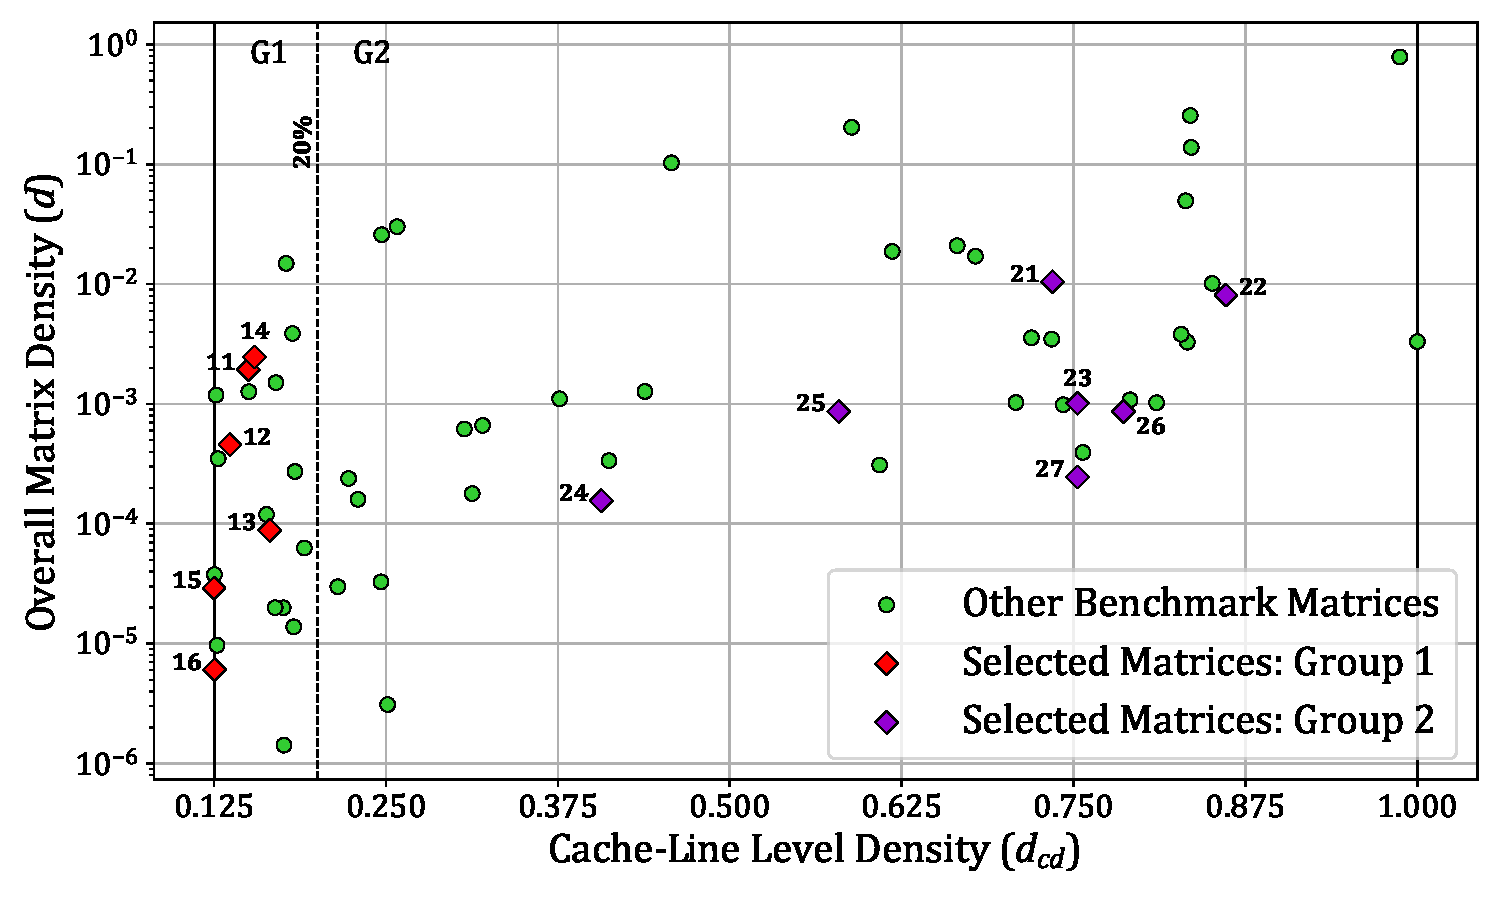
\includegraphics[width=\linewidth]{Chapter_MicroArch/Figures/PDF/BenchmarkMatricesDcdRep.pdf}
    \caption{Benchmark Matrices: $d_\mathit{cd}$ vs $nnz/Column$}
    \label{fig:arch:matrices}
\end{figure}

\begin{highlight}{Conclusion}{Red}
    The benchmark matrices are divided into two groups depending on $d_\mathit{cd}$, their average cache-line-sized clusters density.
\end{highlight}

% %%%%%%%%%%%%%%%%%%%%%%%%%%%%%%%%%%%%%%%%%%%%%%%%%%%%%%%%%%%%%%%%%%%%%
\subsection{Results Analysis}

% %%%%%%%%%%%%%%%%%%%%%%%%%%%%%%%%%%%%%%%%%%%%%%%%%%%%%%%%%%%%%%%%%%%%%
\subsubsection{Memory Traffic}

For all the benchmark matrices, we simulated the SystemVerilog model executing the full \algo{OP} SpMV and initially measured the memory traffic for the output vector as shown in Figure~\ref{fig:arch:outmemtraffbar} for \textit{RedC}, OBaMMA with BaCSC and OBaMMA with CSC.
These results are expressed as a ratio compared to the memory traffic for \textit{GC}.
OBaMMA achieves a remarkable $3.9\times$ reduction in memory traffic which is over $2.7\times$ lower compared to \textit{RedC}. 
OBaMMA performs well for the matrices in both groups.
Since \textit{GC} performs better for group~2, the relative benefit of OBaMMA is smaller but still significant.
With OBaMMA, the data in the DRC is dense and stays in the cache from column to column enabling the rotating pattern of Section~\ref{sec:theory} to occur.
Outside of the DRC, the opportunities for reuse are limited and the element-wise, fully-associative storage makes best use of the memory bandwidth by avoiding the transfer of mostly empty cache-lines.

Note that for the group~1 matrices, the \textit{RedC} traffic is higher than for \textit{GC}.
Indeed, when the cache-lines are always sparsely used, the cache is ineffective, both for \textit{GC} and \textit{RedC}.
In our configuration, the size of \textit{GC} is 2$\times$ larger than the DRC region in the \textit{RedC}, which explains the better performance.
For the group~2 matrices, the cache becomes effective, as the cache-lines frequently hit, and it becomes possible to take advantage of the in-memory accumulation provided by \textit{RedC}.

So far, we focused on output memory traffic.
To perform an \algo{OP} SpMV, the input matrix and input vector are read once in a linear fashion~\cite{Isaac2024_SoA}.
Figure~\ref{fig:arch:inoutmetraff} shows the distribution of the total memory traffic including inputs and the output vector.
We note the stark difference in behavior between the group~1 and group~2 matrices.
For group~1, with traditional caches, the output traffic is high because near empty cache-lines are frequently transferred back and forth to main memory and, this is one of the reasons that \algo{OP} algorithms are less used, despite having theoretically better performance~\cite{Mukkara2019_PHI, Isaac2024_SoA}.
For these matrices, OBaMMA greatly reduces the output traffic providing a $2.7\times$ reduction in overall traffic.
For the group~2 matrices, OBaMMA still provides a $17\%$ reduction in overall traffic, although these matrices already perform well with traditional caches.
For \textit{GC}, \textit{RedC} and OBaMMA with CSC, the volume of input traffic is constant. 
With OBaMMA, the preprocessing adds a small input traffic overhead ($< 10\%$).

\begin{figure}[htbp]
    \centering
    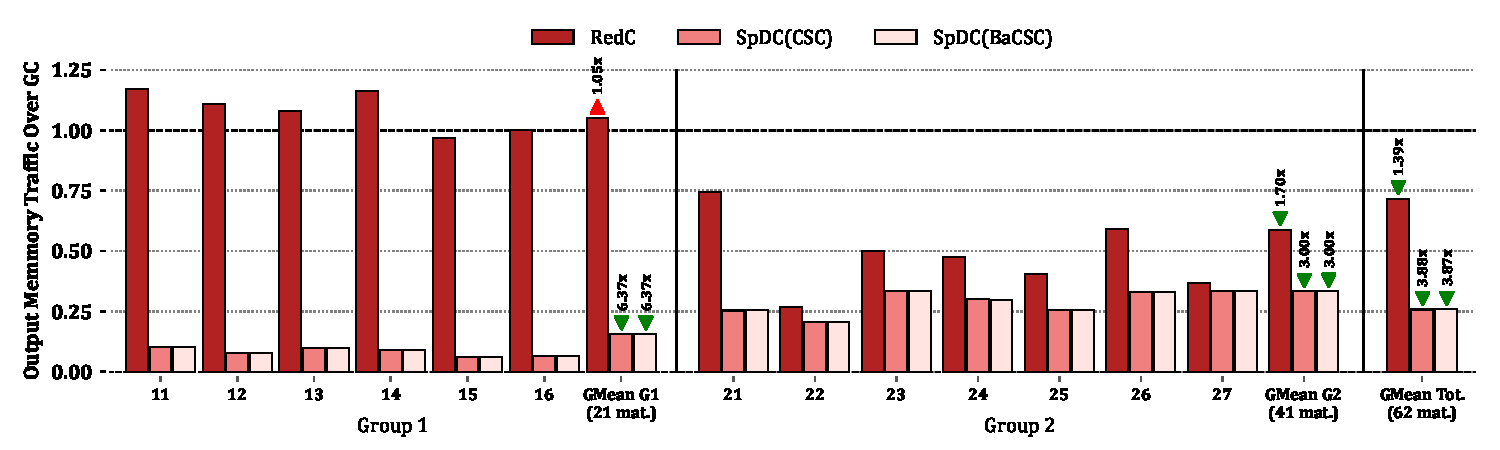
\includegraphics[width=\linewidth]{Chapter_MicroArch/Figures/PDF/OutMemTrafficFromRTL.pdf}
    \caption{Output Memory Traffic Normalized over \acrshort{gc}, from \acrshort{rtl} Simulations}
    \label{fig:arch:outmemtraffbar}
    % \label{fig:arch:outMT}
\end{figure}

\begin{figure}[htbp]
    \centering
    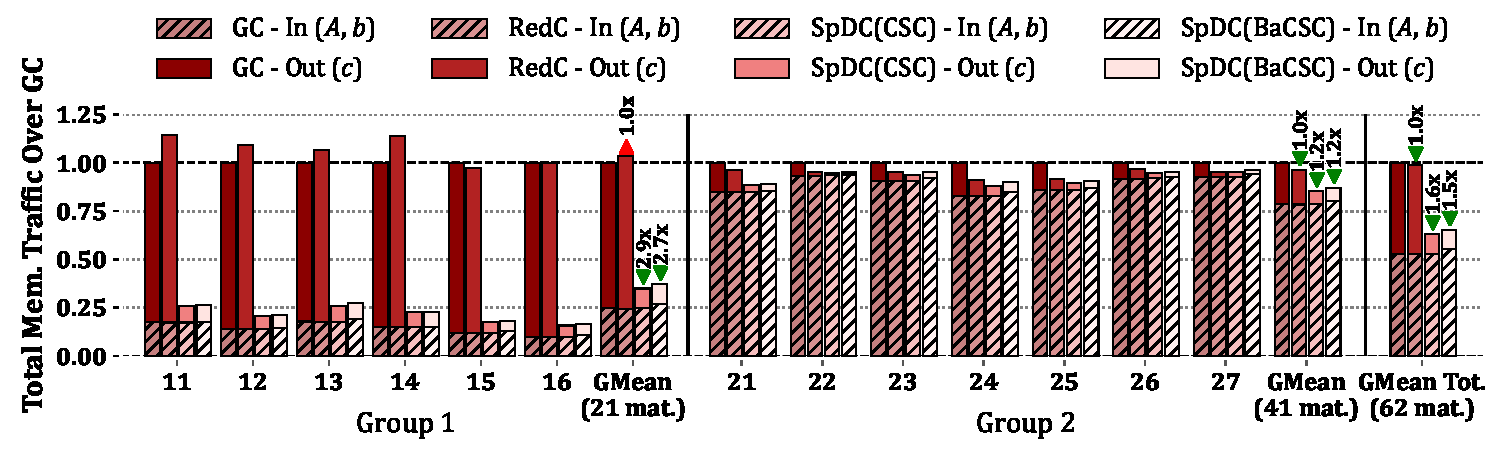
\includegraphics[width=\linewidth]{Chapter_MicroArch/Figures/PDF/TotMemTrafficFromRTL.pdf}
    \caption{Total Memory Traffic on Input Matrix $A$, Input Vector $b$ and Output Vector $c$, Normalized over \acrshort{gc}, from \acrshort{rtl} Simulations}
    \label{fig:arch:inoutmetraff}
    % \label{fig:arch:totMT}
\end{figure}

% %%%%%%%%%%%%%%%%%%%%%%%%%%%%%%%%%%%%%%%%%%%%%%%%%%%%%%%%%%%%%%%%%%%%%
\subsubsection{Latencies}

Our focus now shifts to the total compute time, and we recall that all main memory reads incur a fixed 64 cycle latency.
Figure~\ref{fig:arch:speedup} shows the speedup compared to execution on \textit{GC}.
For the group~1 matrices, we first note that \textit{RedC} achieves some speedup $(1.09\times$) which can be explained as the RED operation is ``fire-and-forget'' for the processor, however, they can quickly block in the cache if the \textit{accumulation table} (\textit{AccTab}) is busy processing the previous request.
In the group~1 matrices, because the cache-lines are sparse, there are frequently bursts of evictions making this effect dominant, thus the system is memory bound.
OBaMMA slightly outperforms \textit{RedC} because it can also issue ``fire-and-forget'' element-wise memory transactions which reduces the blocking.

For the group~2 matrices, particularly, with our single core RISC-V processor, the system becomes compute bound.
For OBaMMA with CSC, there is an overhead to calculate the region which results in some slow down ($-1.36\times$), however, with preprocessing, this overhead is removed and OBaMMA achieves the same latencies as \textit{GC}.

\begin{figure}[htbp]
    \centering
    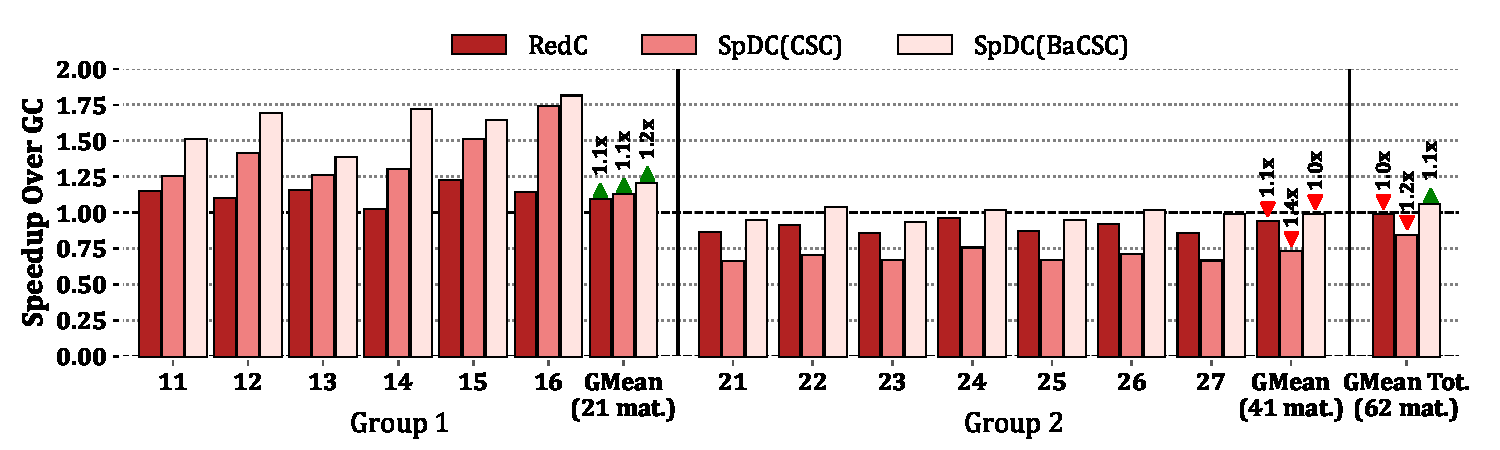
\includegraphics[width=\linewidth]{Chapter_MicroArch/Figures/PDF/Speedups.pdf}
    \caption{Speedup over \acrshort{gc}, from \acrshort{rtl} Simulations}
    \label{fig:arch:speedup}
\end{figure}

% %%%%%%%%%%%%%%%%%%%%%%%%%%%%%%%%%%%%%%%%%%%%%%%%%%%%%%%%%%%%%%%%%%%%%
\subsubsection{Discussion over the Two Performance Groups}

%discussion using slide

Two parameters characterize sparse matrices: (1) the $nnz/Column$ which is a coarse-grain measure of density and (2) the $d_\mathit{cd}$ which is a measure of the density at the granularity of a cache-line.
In Figure~\ref{fig:arch:allscatter}, the normalized memory traffic ($bytes/nnz$) for each of the matrices is shown for \textit{RedC} and OBaMMA.
With \textit{RedC}, the memory traffic is high for low values of $d_\mathit{cd}$ whereas for OBaMMA, the memory traffic is virtually independent of both density parameters.

\begin{figure}[htbp]
    \centering
    \begin{subfigure}{0.49\linewidth}
        \centering
        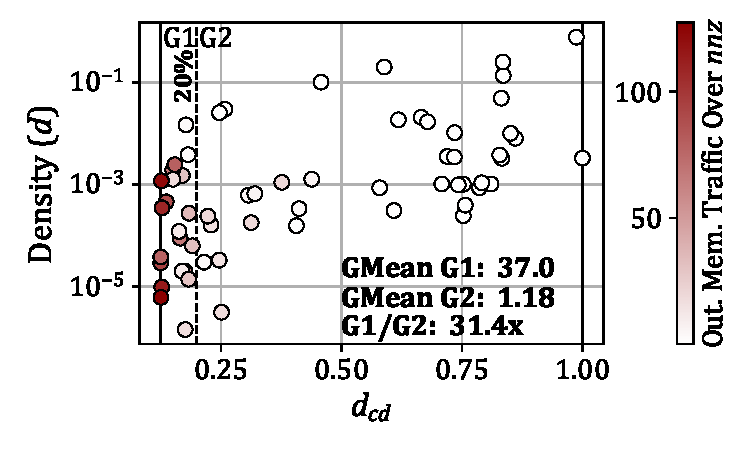
\includegraphics[width=\linewidth]{Chapter_MicroArch/Figures/PDF/MatricesDcdRep_WithMT_onRedC.pdf}
        \caption{\acrshort{redc} Output Memory Traffic over \acrshort{gc}}
        \label{fig:arch:perfOnMat:00}
    \end{subfigure}
    \hfill
    \begin{subfigure}{0.49\linewidth}
        \centering
        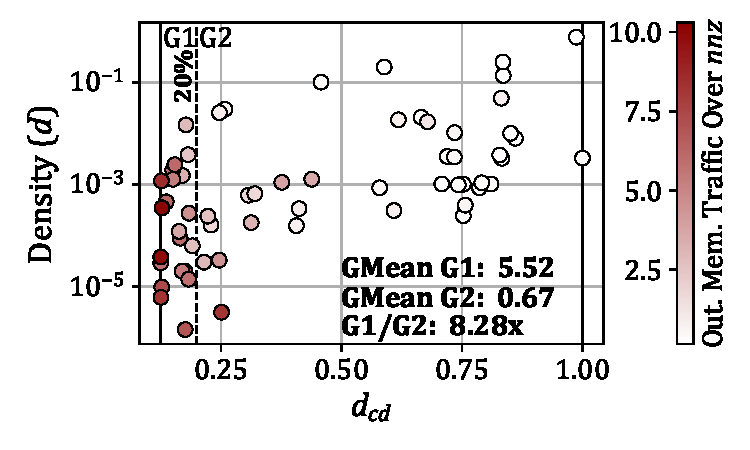
\includegraphics[width=\linewidth]{Chapter_MicroArch/Figures/PDF/MatricesDcdRep_WithMT_onSpDC.pdf}
        \caption{\acrshort{spdc} Output Memory Traffic over \acrshort{gc}}
        \label{fig:arch:perfOnMat:01}
    \end{subfigure}
    %
    \begin{subfigure}{0.49\linewidth}
        \centering
        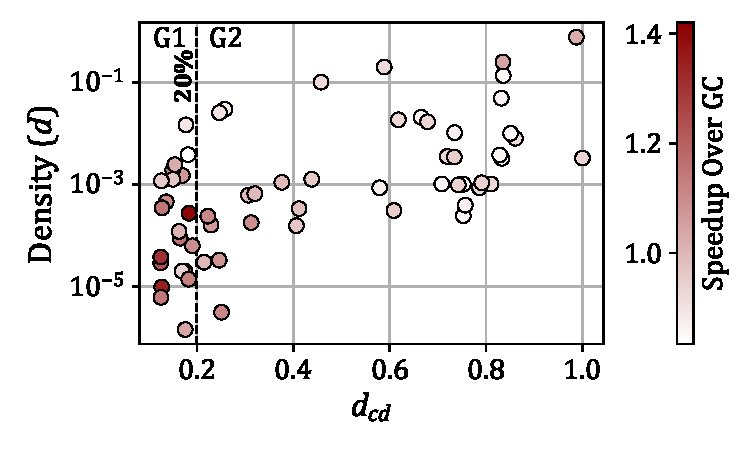
\includegraphics[width=\linewidth]{Chapter_MicroArch/Figures/PDF/MatricesDcdRep_WithSpeedUp_onRedC.pdf}
        \caption{\acrshort{redc} Speedup over \acrshort{gc}}
        \label{fig:arch:perfOnMat:10}
    \end{subfigure}
    \hfill
    \begin{subfigure}{0.49\linewidth}
        \centering
        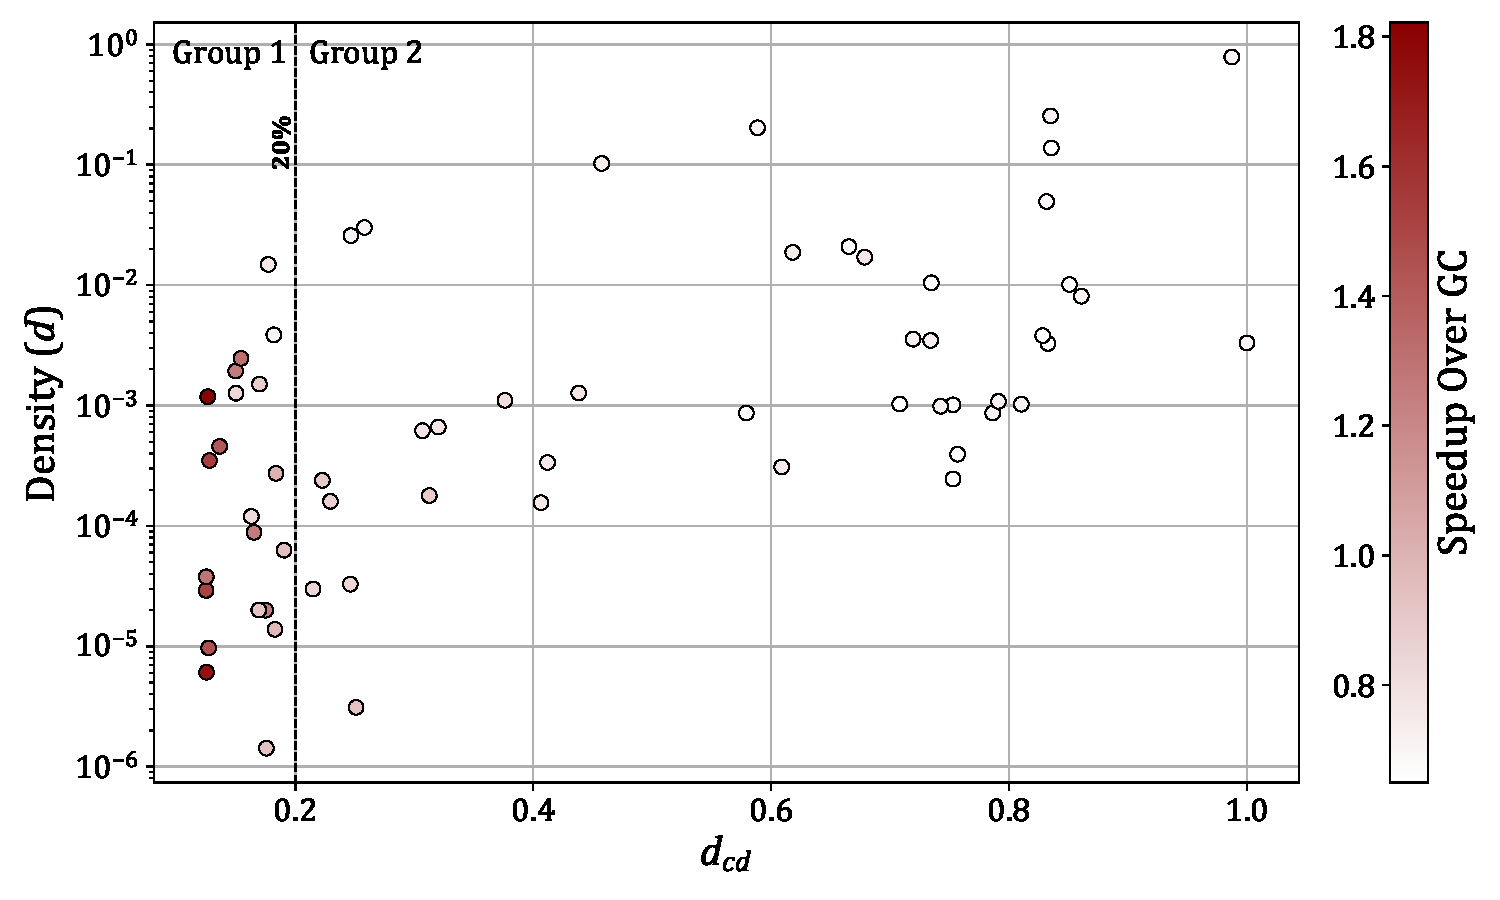
\includegraphics[width=\linewidth]{Chapter_MicroArch/Figures/PDF/MatricesDcdRep_WithSpeedUp_onSpDC.pdf}
        \caption{\acrshort{spdc} Speedup over \acrshort{gc}}
        \label{fig:arch:perfOnMat:11}
    \end{subfigure}
    \caption{Memory Traffic and Speedup Performance Visualized Across Benchmark Matrix Densities and $d_\mathit{cd}$}
    \label{fig:arch:perfOnMat}
\end{figure}

To summarize, the group~1 matrices are the ones that perform poorly with traditional caches, and for this group, OBaMMA achieves a $2.4\times$ reduction in memory traffic and a speedup of $1.21\times$.
In a processor with more compute resources (e.g. multicore) the pressure on the memory system would be greater and the majority of matrices would behave as the group~1 matrices.
Indeed, with OBaMMA, the memory traffic is insensitive to the characteristics of the matrices as shown in Figure~\ref{fig:arch:allscatter} which makes for predictable performance.

We previously discussed how the single-entry \textit{AccTab} was a performance bottleneck for \textit{RedC}. 
We investigate the impact of increasing the \textit{AccTab} entries from 1 to 8, presenting the speedup relative to \textit{GC} for selected group~1 and~2 matrices.

For the matrices in group~2, which are compute bound, increasing the \textit{AccTab} entries has no impact on runtime ($\leqslant 1\%$).
In the case of group~1 matrices, setting the \textit{AccTab} to 1, 2, 4, and 8 entries allows \textit{RedC} to achieve performance improvements of $1.16\times$, $1.36\times$, $1.60\times$, and $1.61\times$ respectively, compared to \textit{GC}, although this comes at the cost of increased area.
For OBaMMA, increasing the \textit{AccTab} has virtually no impact regardless of the matrices ($\leqslant 0.5\%$).
This is expected as there are rarely evictions from the DRC as it is sized to contain the \gls{band}.
OBaMMA's region based architecture thus reduces both total memory traffic and memory bursts.

% %%%%%%%%%%%%%%%%%%%%%%%%%%%%%%%%%%%%%%%%%%%%%%%%%%%%%%%%%%%%%%%%%%%%%
\subsubsection{Area Overhead}

Both HPDcache and OBaMMA systems were synthesized in GF22FDX technology using Synopsis DC\texttrademark.
The original area was $0.99~mm^2$ and the OBaMMA version was $1.3~mm^2$, an increase of $26\%$.
This shows that OBaMMA could reasonably be integrated into a processor, providing a large performance improvement ($3.9\times$ in memory traffic), with an area overhead that is much lower than predicted by Borkar's law~\cite{Borkar2007_AreaOverheads}.
% GC 991638,916 um2 / OBaMMA 1252208,92 um2 / 26%

% %%%%%%%%%%%%%%%%%%%%%%%%%%%%%%%%%%%%%%%%%%%%%%%%%%%%%%%%%%%%%%%%%%%%%
\subsection{Comparison with the Analytical Model}

To validate consistency between our models and implementations, we compare the normalized output memory traffic produced by three sources: the analytical model of Chapter~\ref{cha:theory}, the Python model of Chapter~\ref{cha:spdc}, and the \acrshort{rtl} implementation presented in this chapter.
For a fair comparison, the caches for \acrshort{redc} and \acrshort{spdc} are configured to 32~KiB total (see Table~\ref{tab:arch:region_configs}): 50\%/50\%/0\% for \acrshort{redc} and 25\%/50\%/25\% for \acrshort{spdc}.
The analytical model accepts global parameters and density distributions rather than concrete matrices, so we synthesize \gls{banded} matrices for the Python and \acrshort{rtl} simulations that match those parameters.
All synthetic matrices use $M = 10^{4}$, half-\gls{band} width $w_\mathit{hB} = 1021$, in-\gls{band} density $d_\mathit{IB} = 10^{-2}$, and out-of-\gls{band} density $d_\mathit{OB}$ varying from $10^{-7}$ to $10^{-2}$.
Note that at $d_\mathit{OB} \simeq 8\times10^{-3}$, approximately one non-zero element exists per column in the out-of-\gls{band} region, whereas at $d_\mathit{OB} \simeq 8\times10^{-7}$, approximately one non-zero element exists in the entire out-of-\gls{band} region, resulting in a nearly \gls{PBanded} matrix.

\begin{figure}[htbp]
    \centering
    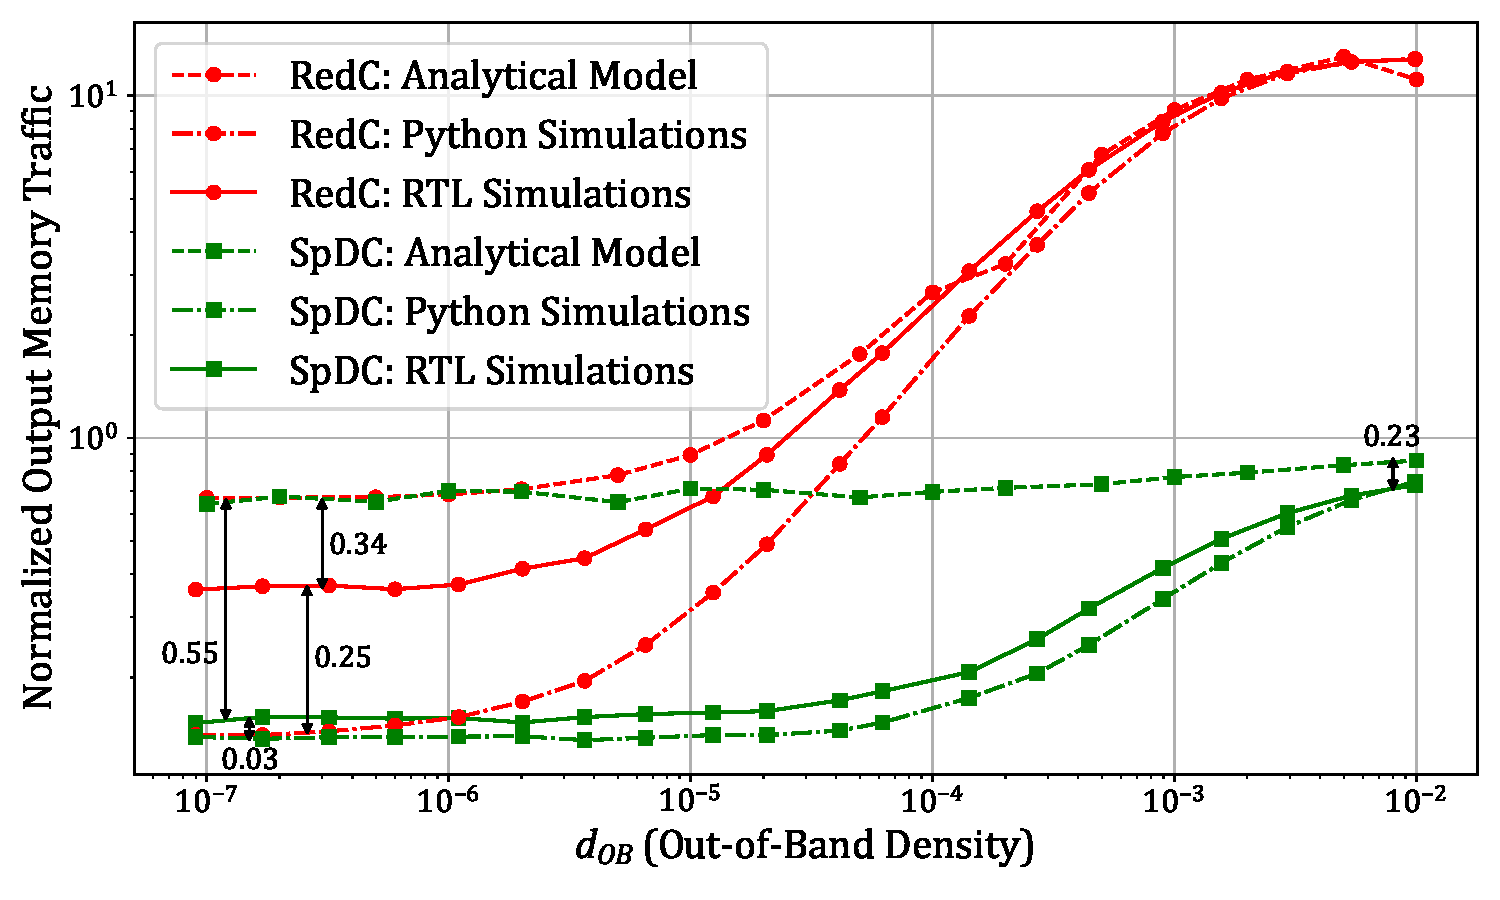
\includegraphics[width=\linewidth]{Chapter_MicroArch/Figures/PDF/graph11_25.12.02.pdf}
    \caption{Normalized Output Memory Traffic Depending on the Out-of-Band Density for the \acrshort{redc} and \acrshort{spdc} Configurations, Through Different Simulation Models}
    \label{fig:arch:graph11}
\end{figure}

Figure~\ref{fig:arch:graph11} shows the results: \acrshort{spdc} (\textit{green}) outperforms \acrshort{redc} (\textit{red}) in normalized output memory traffic ($\mathit{normMT}$).
Two observations are noteworthy.
First, the three approaches agree most closely when $d_\mathit{OB}$ is low.
Indeed, at $d_\mathit{OB} = 10^{-2}$ there is no measurable difference for \acrshort{redc}, while \acrshort{spdc} exhibits a 0.23 difference in $\mathit{normMT}$.
At the smallest $d_\mathit{OB}$ the discrepancies reach 0.58 element transferred in memory per \gls{reduction}.
Overall trends are preserved across models and deviations remain small.
Second, the analytical model consistently overestimates traffic, the Python model consistently underestimates it, and the \acrshort{rtl} results fall between the two.

\begin{highlight}{Conclusion}{Red}
    Across synthetic \gls{banded} matrices, all three simulation models demonstrate consistent memory traffic results, with only minor divergences as matrices approach the \gls{PBanded} regime.
\end{highlight}

% %%%%%%%%%%%%%%%%%%%%%%%%%%%%%%%%%%%%%%%%%%%%%%%%%%%%%%%%%%%%%%%%%%%%%
\subsection{Comparison with the Python Model}

To further validate our implementation over real, not necessarily \gls{banded}, matrices, we compare the \acrshort{rtl} results against the Python simulations from Chapter~\ref{cha:spdc}.
Table~\ref{tab:arch:results_python} presents the Python results for the \acrshort{rtl} cache configurations shown in Table~\ref{tab:arch:region_configs}.
We include the \acrshort{redc} 50\%/50\%/0\% configuration for comparison, though it is suboptimal according to the Python analysis.
Table~\ref{tab:arch:rtl_vs_python} reports \acrshort{rtl} results with geometric mean over the same 48 matrices used in Python simulations, comparing output and total memory traffic.

\begin{figure}[htbp]
    \centering
    \begin{minipage}[t]{0.49\linewidth}
        \centering
        \begin{table}[H]
            \caption{Results of Main Cache Configurations from Python Simulation}
            \label{tab:arch:results_python}
            \centering
            \begin{tblr}{
                    width = {0.88\linewidth},
                    colspec = {X[1.7,c] X[0.5,c] X[0.8,c] *{3}{X[c]}}, % rowspec
                    rows = {m, font=\small},
                    colsep = {1pt},
                    column{1-3} = {colsep=0pt},
                    column{1} = {leftsep=1pt},
                    column{3} = {rightsep=1pt},
                    row{1-Z} = {rowsep=2pt, black!2},
                    row{1} = {c, font=\bfseries\small, black!5},
                    column{1} = {l},
                    row{2-4} = {c, black!5},
                    row{2-4} = {font=\itshape\small},
                    row{2-4} = {rowsep=0pt},
                    row{6,9,11,13} = {abovesep=0pt},
                    row{5,8,10,12} = {belowsep=0pt},
                    cell{2}{2} = {r=3}{c},
                    cell{2-4}{1} = {r},
                    cell{5,8,10,12}{1} = {r=2}{},
                    cell{5-13}{1} = {c=3}{},
                    cell{1}{1} = {r=2}{},
                    hspan = {minimal},
                    % hlines, vlines,
                    % rulesep = {-1pt},
                    hline{1,Z} = {2pt}, % Z for last
                    hline{5} = {1pt},
                    vline{4} = {1-Z}{0.5pt},
                }
                %
                GMeans (48 mat.) & & & \acrshort{gc} & \acrshort{redc} & \acrshort{spdc} \\
                %
                & \rotatebox[y=2pt]{90}{\glspl{set}} & \acrshort{grc}\; & 128 & 64 & 32 \\
                &                                    & \acrshort{drc}\; & \O  & 64 & 64 \\
                &                                    & \acrshort{srt}\; & \O  & \O & 32 \\
                %
                \textbf{Output Memory Traffic} (\% over GC)      & & & 100  & 103 & 24.5 \\
                                                                & & & \cst1.0 & \cst1.0 & \dwG4.1 \\
                \textbf{Ratio of RMWs in Memory Traffic} (\%)    & & & \O   & \O   & 40.5 \\
                \textbf{Total Memory Traffic} (\% over GC)       & & & 100  & 98.5 & 56.1 \\
                                                                & & & \cst1.0 & \cst1.0 & \dwG1.8 \\
                \textbf{Evicted Cache Line Utilization} (max: 8) & & & 3.60 & 3.41 & 7.21 \\
                                                                & & & \cst1.0 & \cst1.0 & \upG2.0 \\
                \textbf{Cache Memory Utilization} (\%)           & & & 36.4 & 43.8 & 75.2 \\
                                                                & & & \cst1.0 & \upG1.2 & \upG2.1 \\
                %
            \end{tblr}
        \end{table}
    \end{minipage}
    \hfill
    \begin{minipage}[t]{0.49\linewidth}
        \centering
        \begin{table}[H]
            \caption{\acrshort{rtl} Results Comparison with Python Simulations}
            \label{tab:arch:rtl_vs_python}
            \centering
            \begin{tblr}{
                    width = {0.88\linewidth},
                    colspec = {X[1.7,c] X[0.5,c] X[0.8,c] *{3}{X[c]}}, % rowspec
                    rows = {m, font=\small},
                    colsep = {1pt},
                    column{1-3} = {colsep=0pt},
                    column{1} = {leftsep=1pt},
                    column{3} = {rightsep=1pt},
                    row{1-Z} = {rowsep=2pt, black!2},
                    row{1} = {c, font=\bfseries\small, black!5},
                    column{1} = {l},
                    row{2-4} = {c, black!5},
                    row{2-4} = {font=\itshape\small},
                    row{2-4} = {rowsep=0pt},
                    row{6,8,10,12} = {abovesep=0pt},
                    row{5,7,9,11} = {belowsep=0pt},
                    cell{2}{2} = {r=3}{c},
                    cell{2-4}{1} = {r},
                    cell{5,7,9,11}{1} = {r=2}{},
                    cell{5-Z}{1} = {c=3}{},
                    cell{1}{1} = {r=2}{},
                    hspan = {minimal},
                    % hlines, vlines,
                    % rulesep = {-1pt},
                    hline{1,Z} = {2pt}, % Z for last
                    hline{5} = {1pt},
                    vline{4} = {1-Z}{0.5pt},
                }
                %
                GMeans (48 mat.) & & & \acrshort{gc} & \acrshort{redc} & \acrshort{spdc} \\
                %
                & \rotatebox[y=2pt]{90}{\glspl{set}} & \acrshort{grc}\; & 128 & 64 & 32 \\
                &                                    & \acrshort{drc}\; & \O  & 64 & 64 \\
                &                                    & \acrshort{srt}\; & \O  & \O & 32 \\
                %
                \textbf{Output Memory Traffic} (\% over GC) & & & 100  & 75.5 & 20.0 \\
                                                            & & & \cst1.0 & \dwG1.3 & \dwG5.0 \\
                $\rightarrow$ \textbf{RTL/Python} (\%)      & & & 116 & 85.0 & 94.6 \\
                                                            & & & \upR0.9 & \dwG1.2 & \dwG1.1 \\
                \textbf{Total Memory Traffic} (\% over GC)  & & & 100  & 99.3 & 54.7 \\
                                                            & & & \cst1.0 & \cst1.0 & \dwG1.8 \\
                $\rightarrow$ \textbf{RTL/Python} (\%)      & & & 75.5 & 76.1 & 73.6 \\
                                                            & & & \dwG1.3 & \dwG1.3 & \dwG1.4 \\
                %
            \end{tblr}
        \end{table}
    \end{minipage}
\end{figure}

The total memory traffic for \acrshort{redc} and \acrshort{spdc} relative to \acrshort{gc} is nearly equivalent across both simulations.
However, output memory traffic shows notable differences: \acrshort{rtl} achieves better traffic reduction than Python, 1.3$\times$ for \acrshort{redc} (vs. 1.0$\times$ in Python) and 5.0$\times$ for \acrshort{spdc} (vs. 4.1$\times$ in Python).
Comparing raw traffic values between \acrshort{rtl} and Python simulations across all configurations, we observe approximately 25\% lower total memory traffic in \acrshort{rtl}.
Output memory traffic varies by $\pm$15\%, with \acrshort{rtl} showing favorable results for both \acrshort{redc} and \acrshort{spdc}.

\begin{highlight}{Conclusion}{Red}
    Over a set of real application matrices, the \acrshort{rtl} implementation corroborates the Python simulations, exhibiting slightly improved memory traffic performance.
\end{highlight}
% %%%%%%%%%%%%%%%%%%%%%%%%%%%%%%%%%%%%%%%%%%%%%%%%%%%%%%%%%%%%%%%%%%%%%
% %% Microarchitecture %%
% Conclusion
% %%%%%%%%%%%%%%%%%%%%%%%%%%%%%%%%%%%%%%%%%%%%%%%%%%%%%%%%%%%%%%%%%%%%%

\section{Conclusion}
\label{sec:arch:conclu}

TODO

\begin{highlight}{Takeaways}{Mulberry}
    \colorbf{Mulberry}{TODO}
\end{highlight}

\clearpage

\clearpage
%%%%%%%%%%%%%%%%%%%%%%%%%%%%%%%%%%%%%%%%%%%%%%%%%%%%%%%%%%%%%%%%%%%%%%%%%
% CHAPTER Optimizations
%%%%%%%%%%%%%%%%%%%%%%%%%%%%%%%%%%%%%%%%%%%%%%%%%%%%%%%%%%%%%%%%%%%%%%%%%

\chapter[Optimizations]{SpDCache Optimizations}
\label{cha:optim}

\minitoc

% %%%%%%%%%%%%%%%%%%%%%%%%%%%%%%%%%%%%%%%%%%%%%%%%%%%%%%%%%%%%%%%%%%%%%
% %% Optims %%
% Introduction
% %%%%%%%%%%%%%%%%%%%%%%%%%%%%%%%%%%%%%%%%%%%%%%%%%%%%%%%%%%%%%%%%%%%%%

\section{Introduction}
\label{sec:optim:intro}

%TODO

\clearpage
% %%%%%%%%%%%%%%%%%%%%%%%%%%%%%%%%%%%%%%%%%%%%%%%%%%%%%%%%%%%%%%%%%%%%%
% %% Optims %%
% RTL Optimizations
% %%%%%%%%%%%%%%%%%%%%%%%%%%%%%%%%%%%%%%%%%%%%%%%%%%%%%%%%%%%%%%%%%%%%%

\section{RTL Optimizations for SpDCache}
\label{sec:optim:rtloptims}

\lettrine{T}{he} \acrshort{rtl} implementation of \acrlong{spdc} presented in Chapter~\ref{cha:arch} was essential to validate our performance models and to analyze performance based on matrix structure.
However, as already noted several times in the previous chapter, the \acrshort{rtl} implementation is missing some features and could be optimized for better practicality and performance.
In this section, we detail the major features and optimizations that are still to be implemented.

% %%%%%%%%%%%%%%%%%%%%%%%%%%%%%%%%%%%%%%%%%%%%%%%%%%%%%%%%%%%%%%%%%%%%%
\subsection{Floating-Point Support Implementation}
\label{sec:optim:rtloptims:fp}

The key focus of this thesis has been the structure on the non-zero elements in the matrix, however, the data-type of the matrices plays an important role in their storage footprint and the arithmetic complexity.
Indeed, in scientific computing, matrices are primarily stored in double precision (64-bits) floating-point.
In other applications such as DNNs or graph analytics, lower precision formats (\ex binary, 16-bits floating-point, 8-bits integer) are frequently used.
To simplify the design complexity of \acrlong{spdc}, we chose to work with 64-bits integer format.
This results in the same data-traffic as double floating-point, but simplifies the design, as the arithmetic operations (accumulations) can be done in a single cycle.
To deploy \acrlong{spdc} for high-performance computing applications, it must be extended to support the double data-type.

To support the accumulation of double format data between \textit{st1} and \textit{st2} in the \gls{pipeline} (Section~\ref{sec:arch:pipeline}), we could either deploy a single-cycle high-performance \acrshort{fpu} with the area trade-offs, or extend the \gls{pipeline} to accommodate two-cycle, for example, floating-point accumulation.
The latter approach better suits our \textit{accumulation table}, which does not stall the \gls{pipeline} and can parallelize element-wise accumulations across stored 64-byte lines.
Additionally, full floating-point support requires extending the AXI port to handle element-wise \acrfull{rmw} operations beyond its native integer capabilities~\cite{ARM2023_AXI}.

Floating-point support is critical for \acrlong{spdc} deployment.
Our expectation is that the associated \acrshort{rtl} changes, while time-consuming, should not present fundamental technical obstacles.

\begin{highlight}{Conclusion}{Red}
    \textbf{Floating-point support} is achievable through \gls{pipeline} extension and requires extending the AXI port for element-wise operations, presenting no fundamental implementation issues.
\end{highlight}

% %%%%%%%%%%%%%%%%%%%%%%%%%%%%%%%%%%%%%%%%%%%%%%%%%%%%%%%%%%%%%%%%%%%%%
\subsection{Region-Sizes Configuration}
\label{sec:optim:rtloptims:config}

One strength of \acrlong{spdc}'s \acrshort{rtl} implementation is its highly configurable design, inherited from the HPDcache implementation used as a foundation.
This allowed us to develop a single \acrshort{rtl} codebase that could be compiled and simulated for multiple designs, \acrshort{gc}, \acrshort{redc}, and \acrshort{spdc}, each with different region size configurations.
However, these configurations are static, requiring \acrshort{rtl} recompilation for each design variant.

Currently, \acrshort{spdc}'s \gls{reduction} mode can be dynamically enabled or disabled via an instruction issued before and after the \acrshort{spmv} kernel.
This switches between a generic cache and a hard-coded \acrshort{rtl} configuration.
To enhance software flexibility, \acrshort{spdc} should support dynamic configuration settings through the initial configuration instruction.

A fundamental limitation is that region sizes are restricted to powers of two, which severely constrains configuration options and led to the 25/50/25\% configuration used in the previous chapter.
This restriction stems from address decoding that uses bit shifts to extract the \gls{set} index, an approach inherited from HPDcache.
Supporting arbitrary region sizes would require integer division and modulo operations, which could introduce long, critical paths.
However, our Python simulations in Chapter~\ref{cha:spdc} demonstrate that precise region sizing is unnecessary for achieving good performance, making this optimization less important.

A practical compromise would be to provide one or two predefined configurations for \acrshort{redc} and \acrshort{spdc}, allowing dynamic selection by software while maintaining a simple user interface.

\begin{highlight}{Conclusion}{Red}
    Dynamic region-size configuration through software, while desirable, has a high hardware complexity without significant performance gains.
    A practical approach is to provide \textbf{predefined configurations for dynamic selection}, balancing flexibility with implementation simplicity.
\end{highlight}

% %%%%%%%%%%%%%%%%%%%%%%%%%%%%%%%%%%%%%%%%%%%%%%%%%%%%%%%%%%%%%%%%%%%%%
\subsection{Hardware Calculation of Region and Band-Width}
\label{sec:optim:rtloptims:regionInHW}

\acrlong{spdc} evaluation shows that depending on matrix characteristics, the \acrshort{op} \acrshort{spmv} kernel can be compute-bound, making region calculation a critical software bottleneck.
We addressed this by using a custom sparse format that converts latency costs into memory traffic costs.
To eliminate any latency or memory traffic overhead, we could compute the region argument of the \acrshort{red} instruction directly in hardware.
This approach sacrifices software flexibility but enables \acrshort{csc} format compatibility and simplifies the \acrshort{op} \acrshort{spmv} kernel to the version shown in Algorithm~\ref{src:arch:op_spmv}.
The required \acrlong{spdc} modifications are:
\begin{itemize}
    \item Configuration: The initial instruction enabling \acrlong{spdc}'s \gls{reduction} mode must accept a configuration argument specifying the word size in bytes ($s_w$), the output vector address ($c$), and the \acrshort{drc} size in bytes ($s_\mathit{DRC}$).
    The hardware could fetch the last parameter independently.
    When this instruction is issued, prior to each \acrshort{spmv}, the half-\gls{bw} is computed and retained until reconfigured, where $s_l$ denotes cache-line size in bytes:
    $$w_\mathit{hB} = \dfrac{s_\mathit{DRC}-s_l}{2 \times s_w}+1$$
    The half-\gls{bw} could also be computed in software, and given as argument to the configuration.
    %
    \item Column indexing: Each outer-loop iteration requires issuing a new instruction containing the current column index $j \in \ldb 0; M-1 \rdb$, denoted $CCOL(j)$.
    This value persists until the next $CCOL$ instruction arrives, consuming one cycle per outer-loop iteration.
    Note that the \acrshort{reg} instruction becomes unnecessary.
    %
    \item Region determination: For each $RED(addr, val)$ instruction, \acrshort{spdc} computes the current row $i \in \ldb 0; M-1 \rdb$ from the address: $i = \dfrac{addr-c}{s_w}$, then determines the region as \acrshort{ibr} if $|i-j| \leqslant w_\mathit{hB}$, otherwise \acrshort{obr}.
\end{itemize}
These modifications impose minimal hardware overhead, with per-\gls{reduction} computations executed at \textit{st0} in the \acrlong{spdc} \gls{pipeline}.
This feature becomes essential when extending \acrshort{spdc} to multi-level, multi-core architectures (Section~\ref{sec:optim:multicore}).

\begin{highlight}{Conclusion}{Red}
    \textbf{Hardware-based region computation} eliminates unnecessary instructions in the software's inner-loop, enabling \acrshort{csc} format compatibility and simplifying the \acrshort{spmv} kernel with minimal hardware overhead.
\end{highlight}

% %%%%%%%%%%%%%%%%%%%%%%%%%%%%%%%%%%%%%%%%%%%%%%%%%%%%%%%%%%%%%%%%%%%%%
\subsection{Complete Inter-Region Cache Coherency}
\label{sec:optim:rtloptims:coherency}

When executing an \acrshort{op} \acrshort{spmv} kernel with \acrlong{spdc}, we assume that the processor issues \acrshort{red} instructions strictly on addresses of the output vector $c$, and that loads and stores are issued only on addresses not in the output vector $c$.
\acrlong{spdc}'s current implementation provides no hardware safeguards if this assumption is violated.
While we provide local coherency between the two \gls{reduction} regions (\acrshort{drc} and \acrshort{srt}) to prevent $c$ address duplication, we lack coherency with the \acrshort{grc}.
A simple detection system could verify that \glspl{reduction} are issued exclusively on addresses within the output vector's range, while other instructions operate outside this range.
PHI~\cite{Mukkara2019_PHI} demonstrates that full coherency is achievable, as required in their design, proving that \glspl{reduction} and generic instructions can safely coexist within the same cache hierarchy.
In \acrlong{spdc}'s case, implementing global inter-region coherency would require the following modifications:
\begin{itemize}
    \item Configuration: When enabling \gls{reduction} mode, the configuration parameter must specify the address range for \acrshort{red} instructions (\eg, output vector $c$ and its extent).
    %
    \item Region Assignment: To prevent address duplication between \gls{reduction} regions and the \acrshort{grc}, loads and stores on $c$ addresses target \gls{reduction} regions, while \acrshortpl{red} on non-$c$ addresses target the \acrshort{grc}.
    The following cases apply only when \gls{reduction} mode is enabled.
    %
    \item Load on $c$ address:
    \begin{itemize}
        \item \Glspl{miss} in \acrshort{drc} and \acrshort{srt}: Issue memory read and return data to processor, bypassing cache.
        \item \Gls{hit} in \acrshort{drc} or \acrshort{srt}: Issue memory read, accumulate with cached data, and return result to processor.
    \end{itemize}
    We do not update \gls{reduction} regions on load to avoid complexity.
    Updating would require writing zeros to memory to prevent double accumulation upon \gls{eviction} or flush.
    %
    \item Store on $c$ address:
    \begin{itemize}
        \item \Glspl{miss} in \acrshort{drc} and \acrshort{srt}: Issue memory write with store value, bypassing cache.
        \item \Gls{hit} in \acrshort{drc} or \acrshort{srt}: Overwrite cached data with store value and issue memory write of a zero to maintain consistency.
    \end{itemize}
    Cache policy (write-through and write-back) can influence this design choice.
    Crucially, data must not exist in both memory and cache simultaneously.
    %
    \item \acrshort{red} on non-$c$ address:
    \begin{itemize}
        \item \Gls{miss} in \acrshort{grc}: Issue memory read, accumulate with \acrshort{red} value, insert into \acrshort{grc} (with \gls{eviction} if needed), and mark dirty (write-back) or write to memory (write-through).
        \item \Gls{hit} in \acrshort{grc}: Accumulate cached data with \acrshort{red} value, update \acrshort{grc} accordingly, and mark dirty (write-back) or write to memory (write-through).
    \end{itemize}
\end{itemize}
It is to be expected that incorrect region usage increases memory traffic and latency, degrading performance.
Implementing a coherency or detection scheme would ensure deterministic behavior, a clear benefit for \acrlong{spdc} deployment.

\begin{highlight}{Conclusion}{Red}
    \textbf{Complete inter-region cache coherency} prevents address duplication across \gls{reduction} and generic regions, ensuring deterministic behavior at minimal hardware cost through address-range configuration and region-specific load/store/reduction handling.
\end{highlight}
% %%%%%%%%%%%%%%%%%%%%%%%%%%%%%%%%%%%%%%%%%%%%%%%%%%%%%%%%%%%%%%%%%%%%%
% %% Optims %%
% SpDCache on MM kernels
% %%%%%%%%%%%%%%%%%%%%%%%%%%%%%%%%%%%%%%%%%%%%%%%%%%%%%%%%%%%%%%%%%%%%%

\section{SpDCache on Matrix-Matrix Multiplication Kernels}
\label{sec:optim:spmm}

%TODO
% %%%%%%%%%%%%%%%%%%%%%%%%%%%%%%%%%%%%%%%%%%%%%%%%%%%%%%%%%%%%%%%%%%%%%
% %% Optims %%
% SpDCache on Multicore Architecture
% %%%%%%%%%%%%%%%%%%%%%%%%%%%%%%%%%%%%%%%%%%%%%%%%%%%%%%%%%%%%%%%%%%%%%

\section{SpDCache on Multi-Level, Multi-Core System}
\label{sec:optim:multicore}

%TODO
% %%%%%%%%%%%%%%%%%%%%%%%%%%%%%%%%%%%%%%%%%%%%%%%%%%%%%%%%%%%%%%%%%%%%%
% %% Optims %%
% Conclusion
% %%%%%%%%%%%%%%%%%%%%%%%%%%%%%%%%%%%%%%%%%%%%%%%%%%%%%%%%%%%%%%%%%%%%%

\section{Conclusion}
\label{sec:optim:conclu}

%TODO

\clearpage

\clearpage

% %%%%%%%%%%%%%%%%%%%%%%%%%%%%%%%%%%%%%%%%%%%%%%%%%%%%%%%%%%%%%%%%%%%%%%%%%%%%%%%%%%%%%%%

% %%%%%%%%%%%%%%%%%%%%%%%%%%%%%%%%%%%%%%%%%%%%%%%%%%%%%%%%%%%%%%%%%%%%%%%%%%%%%%%%%%%%%%%
%                             Post Sections
% %%%%%%%%%%%%%%%%%%%%%%%%%%%%%%%%%%%%%%%%%%%%%%%%%%%%%%%%%%%%%%%%%%%%%%%%%%%%%%%%%%%%%%%
% Conclusion
% %%%%%%%%%%%%%%%%%%%%%%%%%%%%%%%%%%%%%%%%%%%%%%%%%%%%%%%%%%%%%%%%%%%%%%%%%%%%%%%%%%%%%%%

\FancyHeadRight{\sectitle}

\renewcommand{\sectitle}{Conclusion}

\phantomsection
\chapter*{\sectitle}
\addstarredchapter{\sectitle}

\minitoc

\newcounter{concluCnt}
\setcounter{concluCnt}{0}
\renewcommand{\thesection}{\arabic{concluCnt}}

% %%%%%%%%%%%%%%%%%%%%%%%%%%%%%%%%%%%%%%%%%%%%%%%%%%%%%%%%%%%%%%%%%%%%%%%%%%%%%%%%%%%%%%%
% Conclu 1

\addtocounter{concluCnt}{1}
\section{TODO}

\lettrine{I}{n} this thesis, we addressed the central question of \colorbf{Mulberry}{how hardware and architectural mechanisms can be designed to efficiently support computation with sparse data, while ensuring scalability, adaptability, and high performance across diverse workloads}.
Our approach focused on the challenges posed by irregular memory access patterns in sparse matrix computations, particularly in the context of the \textbf{\acrfull{op} \acrfull{spmv}} kernel.
We identified that the \acrshort{op} algorithm, while promising for parallelism and optimization with \acrshort{mv} kernels, generates ``random'' \glspl{reduction} (irregular updates on the output vector) that stress traditional memory systems.
To mitigate these challenges, we proposed \textbf{\acrlong{spdc}}, a novel \textbf{region-based \gls{redC}} architecture designed to optimize memory transactions for sparse data by leveraging the structural properties of \gls{banded} matrices.

Through this work, we developed a \textbf{lightweight, flexible solution} that can be integrated into any kernel suffering from ``random'' \glspl{reduction}, recognizing that caches are a fundamental component of memory hierarchies in CPUs, GPUs, and accelerators.
Our design prioritizes \textbf{scalability}, ensuring that the solution remains effective across different system scales.
Additionally, we addressed the critical influence of \textbf{matrix structure} on performance, conducting a detailed analysis of cache behavior specifically for \gls{banded} matrices.
By adapting our architecture to better handle dense and sparse regions, we provided insights into how matrix structure can inform the design of efficient architectures, with \textbf{\acrlong{spdc}} serving as a practical example.
This work also demonstrated how \textbf{simple yet targeted modifications} to cache design can yield significant performance improvements for \gls{reduction}-based kernels.

While our approach has limitations, such as the absence of a full evaluation on multi-level, multi-core systems and the early-stage refinement of \acrlong{spdc}, we intentionally focused on \textbf{precision and conceptual clarity} over raw performance metrics.
This emphasis on intrinsic understanding, rather than merely achieving impressive results, offers a more meaningful response to our central question and addresses a gap often overlooked in existing accelerator research.

\subsection*{Summary of Contributions}

\paragraph*{Chapter~\ref{cha:background}. Analysis of Sparse Data Computing}

We established a foundational understanding of sparse matrices, their storage formats, and the hardware challenges associated with their computation.
Our analysis of \textbf{\acrfull{ip}, \acrfull{op}, and \acrfull{gust}} algorithms revealed that \acrshort{op} and \acrshort{gust} are the most promising for hardware acceleration, particularly due to their potential for parallelism and data reuse.
We identified \textbf{\gls{gather} (\gls{intersection} searches)} and \textbf{\gls{scatter} (``random'' \glspl{reduction})} as the two core challenges in sparse matrix processing, which guided our subsequent architectural choices.

\paragraph*{Chapter~\ref{cha:soa}. Survey and Classification of State-of-the-Art Accelerators}
We conducted a comprehensive review of recent hardware accelerators for sparse matrix computations, categorizing them based on **autonomy, memory hierarchy position, algorithm compatibility, and hardware support for gather/scatter operations**. Our comparative analysis highlighted that **Gustavson-based accelerators** often achieve the best performance due to their balanced approach to input reuse and output generation. This survey informed the design of **SpDCache**, positioning it as a **processor-assist, near-cache accelerator** optimized for **OP SpMV kernels**.

\paragraph*{Chapter~\ref{cha:spdc}. Design of SpDCache for "Random" Reductions}
We introduced **SpDCache**, a **region-based reduction cache** that partitions memory into **In-Band (IBR) and Out-of-Band (OBR) regions** to optimize handling of both dense and sparse data. Our **Python-based simulation model** demonstrated that SpDCache significantly reduces memory traffic compared to generic caches, particularly for **banded matrices**. The architecture’s **virtual partitioning** and **reduction support** enable efficient management of irregular updates, addressing the scatter problem inherent in OP algorithms.

\paragraph*{Chapter~\ref{cha:theory}. Probabilistic Modeling and Exploration of Cache Behavior}
We developed a **hybrid probabilistic and analytical model** to simulate SpDCache’s behavior during OP SpMV operations. This model allowed us to explore how different cache configurations impact memory traffic, particularly for **banded matrices**. Our analysis revealed **two distinct groups of matrices** based on their **fine-grain structure**, as measured by the **$d_{CD}$ metric** (density of non-zero elements in the central diagonal region). This distinction underscores the importance of **adapting cache regions** to the specific structure of the input matrices.

\paragraph*{Chapter~\ref{cha:arch}. Microarchitecture and RTL Evaluation}
We detailed the **microarchitectural implementation of SpDCache**, featuring **three dedicated regions: Generic Region Cache (GRC), Dense Region Cache (DRC), and Sparse Region Table (SRT)**. Our **RTL simulations** validated the architecture’s effectiveness, showing **significant reductions in memory traffic** and **improved cache utilization**. The results confirmed that SpDCache efficiently handles both **coarse-grain** (region-based partitioning) and **fine-grain** (matrix structure-dependent) optimizations, making it adaptable to a wide range of sparse matrices.

\paragraph*{Chapter~\ref{cha:optim}. Optimizations and Future Directions}
We explored **RTL-level optimizations** to refine SpDCache’s performance, including **multi-core integration** and **extensions to SpMSpM kernels**. These enhancements position SpDCache as a **scalable, versatile solution** for modern sparse matrix processing systems. Our findings lay the groundwork for future research in **high-performance, energy-efficient architectures** for sparse data computations, with a focus on **bandwidth efficiency** and **adaptability to diverse workloads**.

---

\subsection*{Key Results and Insights}

- **Algorithmic Choice:** OP and Gust algorithms are the most effective for hardware acceleration, with **Gustavson offering the best trade-off** for SpMSpM kernels.
- **Cache Optimization:** SpDCache’s **region-based partitioning** and **reduction support** significantly reduce memory traffic, particularly for matrices with **structured sparsity** (e.g., banded matrices).
- **Fine-Grain Structure Matters:** The **$d_{CD}$ metric** revealed two distinct matrix groups, highlighting the need for **adaptive cache configurations** tailored to matrix structure.
- **Scalability and Usability:** SpDCache’s **multi-core extensions** and **optimizations for SpMSpM** demonstrate its potential for **scalable, high-performance sparse matrix processing**.

---

\subsection*{Future Work}

While SpDCache advances the state-of-the-art in cache architectures for sparse data, several avenues remain for future exploration:
- **Multi-Level Cache Hierarchies:** Extending SpDCache to **multi-level cache systems** could further improve performance for large-scale applications.
- **Dynamic Region Sizing:** Implementing **runtime-adaptive region sizing** based on matrix structure could enhance flexibility and efficiency.
- **Integration with Emerging Technologies:** Exploring SpDCache’s compatibility with **in-memory computing** and **processing-in-memory (PIM)** architectures may unlock new performance gains.
- **Broader Application Domains:** Evaluating SpDCache in **graph analytics, deep learning, and scientific computing** could demonstrate its versatility across diverse sparse workloads.

---

\subsection*{Final Thoughts}

This thesis contributes a **novel, reduction-aware cache architecture** that bridges the gap between theoretical insights and practical hardware implementations for sparse matrix computing. By addressing the challenges of **irregular memory accesses** and **efficient data reuse**, SpDCache provides a **scalable, adaptable solution** for modern computational demands. As sparse data continues to grow in importance across scientific, machine learning, and graph analytics applications, architectures like SpDCache will play a critical role in enabling **high-performance, energy-efficient processing** of these challenging workloads.


%%%%%%%%%%%%%%%









Our contributions include:
- **A comprehensive analysis of sparse matrix algorithms and hardware challenges**, highlighting the inefficiencies of traditional caches in handling irregular accesses and reductions.
- **The design and evaluation of SpDCache**, which partitions memory into **In-Band (IBR) and Out-of-Band (OBR) regions** to efficiently manage both dense and sparse data, significantly reducing memory traffic compared to generic caches.
- **Theoretical and probabilistic modeling** to analyze cache behavior, revealing the importance of **fine-grain matrix structure** (measured by the $d_{CD}$ metric) in optimizing performance.
- **Microarchitectural implementation and RTL simulations**, validating SpDCache’s effectiveness in reducing memory traffic and improving cache utilization, while identifying two distinct groups of matrices with different performance profiles.
- **Optimizations and extensions** for multi-core systems and SpMSpM kernels, positioning SpDCache as a scalable solution for modern sparse matrix processing.

However, our work has some limitations:
- **Single-core, single-cache level focus**: Our evaluation was constrained to a single-core, single-cache level system, which limits raw performance compared to more complex, multi-level, or multi-core architectures.
- **Uniformity assumptions**: The analytical model assumes a uniform distribution of non-zero elements, which may not always reflect real-world matrix structures, potentially affecting performance predictions.
- **Hardware complexity**: The fully-associative nature of the Sparse Region Table (SRT) and specialized eviction policies introduce hardware complexity, which could impact scalability and implementation costs.
- **RTL implementation optimization**: The current RTL implementation is a first iteration and could be further refined, as some features are still missing or not fully optimized.

While SpDCache advances the state-of-the-art in cache architectures for sparse data, future work could explore **multi-level cache hierarchies, dynamic region sizing, and integration with emerging technologies** like in-memory computing to further enhance performance and scalability. Additionally, broader application domains, such as graph analytics and deep learning, could be investigated to demonstrate SpDCache’s versatility across diverse sparse workloads.


% \subsection{A Section}

% \subsubsection{A Subsection}

% \lipsum[3]

% %%%%%%%%%%%%%%%%%%%%%%%%%%%%%%%%%%%%%%%%%%%%%%%%%%%%%%%%%%%%%%%%%%%%%%%%%%%%%%%%%%%%%%%
% Conclu 2

% \addtocounter{concluCnt}{1}
% \section{Second element}

% \lipsum[1-5]

% %%%%%%%%%%%%%%%%%%%%%%%%%%%%%%%%%%%%%%%%%%%%%%%%%%%%%%%%%%%%%%%%%%%%%%%%%%%%%%%%%%%%%%%

\renewcommand{\thesection}{\arabic{chapter}.\arabic{section}}

\cleardoublepage %% Comment this line if this section occupies the last pages
% \adjustmtc %% Commented for the appendices minitoc to not disappear
% %%%%%%%%%%%%%%%%%%%%%%%%%%%%%%%%%%%%%%%%%%%%%%%%%%%%%%%%%%%%%%%%%%%%%%%%%%%%%%%%%%%%%%%
% French Synthesis
% %%%%%%%%%%%%%%%%%%%%%%%%%%%%%%%%%%%%%%%%%%%%%%%%%%%%%%%%%%%%%%%%%%%%%%%%%%%%%%%%%%%%%%%

\FancyHeadRight{\sectitle}

\renewcommand{\sectitle}{Synth\`ese en Fran\c cais}

\begin{otherlanguage}{french}

\phantomsection
\chapter*{\sectitle}
\addstarredchapter{\sectitle}

\mtcselectlanguage{french}
\minitoc

\newcounter{synthFCnt}
\setcounter{synthFCnt}{0}
\renewcommand{\thesection}{\arabic{synthFCnt}}

% %%%%%%%%%%%%%%%%%%%%%%%%%%%%%%%%%%%%%%%%%%%%%%%%%%%%%%%%%%%%%%%%%%%%%%%%%%%%%%%%%%%%%%%

\addtocounter{synthFCnt}{1}
\section{Introduction}

\lettrine{C}{ette} thèse aborde un défi central dans le domaine du traitement des données creuses, omniprésentes dans des applications exigeantes comme le calcul scientifique, l'analyse de graphes et l'apprentissage automatique : comment concevoir des mécanismes matériels et architecturaux efficaces pour supporter ces calculs, tout en garantissant scalabilité, adaptabilité et haute performance~?
Les matrices creuses, bien que réduisant considérablement l'empreinte mémoire grâce à des formats compressés (comme \acrshort{csr} ou \acrshort{csc}), posent des défis majeurs en raison de leurs accès mémoire irréguliers.
Ces derniers limitent l'efficacité des caches traditionnels et compliquent la parallélisation des calculs.

Pour répondre à cette problématique, ce manuscrit propose une analyse approfondie des algorithmes fondamentaux de multiplication de matrices creuses, \acrfull{ip}, \acrfull{op} et \acrfull{gust}, et identifie leurs défis matériels respectifs, séparés en deux problèmes clés : le \gls{gather} (recherche d'intersections entre éléments non nuls) et le \gls{scatter} (réductions, c.à.d. lecture-accumulation-écritures, aléatoires sur les résultats).
L'algorithme de \acrlong{gust} émerge comme le plus prometteur pour une implémentation matérielle, grâce à ses compromis équilibrés entre réutilisation des données et génération séquentielle des résultats, tandis que l'\acrshort{op} se révèle particulièrement adapté aux noyaux \acrshort{spmv} (multiplication matrice creuse-vecteur).

La contribution principale de cette thèse est \acrlong{spdc}, une architecture de cache de réduction basée sur des régions, optimisant les transactions mémoire pour les données creuses en exploitant les propriétés structurelles des matrices bandées.
\acrlong{spdc} partitionne la mémoire cache en régions dédiées aux zones denses et creuses, réduisant significativement le trafic mémoire par rapport aux caches génériques.
Les contributions clés incluent :
\begin{itemize}
    \item Une modélisation architecturale via des modèles Python et probabilistes (en C) pour analyser les transactions mémoire et explorer le dimensionnement des caches, mettant en lumière l'importance de la structure gros grain des matrices (comme les bandes denses).
    \item Une implémentation microarchitecturale validée par des simulations \acrshort{rtl}, mettant en lumière l'importance de la structure petit grain des matrices (influençant la densité des lignes de cache).
    \item Des optimisations pour la scalabilité, incluant des extensions aux noyaux de calcul matrice-matrice creuses et des architectures multi-c\oe{}urs.
\end{itemize}

Ce travail fait progresser l'état-de-l'art des architectures de cache pour données creuses, en insistant sur une compréhension intrinsèque des structures matricielles et une conception adaptative pour des solutions matérielles hautes performances.
Dans les sections suivantes, une synthèse pour chaque chapitre du manuscrit résume les travaux effectués, les contributions et les résultats majeurs.

% %%%%%%%%%%%%%%%%%%%%%%%%%%%%%%%%%%%%%%%%%%%%%%%%%%%%%%%%%%%%%%%%%%%%%%%%%%%%%%%%%%%%%%%

\addtocounter{synthFCnt}{1}
\section{Synthèse du Chapitre~\ref{cha:background} : Contexte sur le calcul des matrices creuses}

\lettrine{L}{e} Chapitre~\ref{cha:background} pose les bases théoriques et pratiques pour comprendre les défis liés au traitement des matrices creuses, omniprésentes dans des domaines tels que le calcul scientifique, l'analyse de graphes et l'apprentissage automatique.
Ces matrices, caractérisées par une majorité d'éléments nuls, nécessitent des formats de stockage compressés (comme \acrshort{coo}, \acrshort{csr} ou \acrshort{csc}, voir la Figure~\ref{fig:bg:FormatEx}) pour réduire leur empreinte mémoire et optimiser leur manipulation.
Cependant, leur structure irrégulière engendre des accès mémoire imprévisibles, limitant l'efficacité des caches traditionnels et compliquant la parallélisation des calculs.

\subsection*{Algorithmes de multiplication de matrices creuses}

Trois algorithmes principaux sont analysés pour les opérations de multiplication matrice-vecteur \acrshort{mv} (\acrshort{spmv}, \acrshort{spmspv} ; $A \times b = c$) et matrice-matrice \acrshort{mm} (\acrshort{spmm}, \acrshort{spmspm}, \acrshort{spgemm} ; $A \times B = C$) :
\begin{itemize}
    \item \acrfull{ip} : Intuitif mais souffrant de recherches d'intersection coûteuses entre les éléments non nuls des matrices/vecteurs d'entrée, surtout lorsque les données sont stockées dans des formats compressés.
    \item \acrfull{op} : Génère des réductions aléatoires sur le vecteur ou la matrice de sortie, stressant le système mémoire en raison d'accès irréguliers et de mises à jour partielles fréquentes.
    \item \acrfull{gust} : Un compromis entre \acrshort{ip} et \acrshort{op}, uniquement pour les opérations \acrshort{mm}, optimisant la réutilisation des données d'entrée (lignes de $B$) et la génération séquentielle des résultats (lignes de $C$), ce qui en fait le candidat le plus adapté pour une implémentation matérielle efficace.
\end{itemize}

Une analyse comparative (Tableau~\ref{tab:bg:AlgosHWComp}) met en évidence les forces et faiblesses de chaque algorithme en termes d'accès mémoire, de parallélisme et de réutilisation des données.
Par exemple, pour des opérations \acrshort{mm}, \acrshort{gust} évite les accès aléatoires sur une matrice entière et réduit significativement le trafic mémoire avec une mémoire locale limitée, contrairement à \acrshort{ip} ou \acrshort{op}.

\subsection*{Défis matériels et solutions}

Les accès irréguliers (\gls{gather} pour \acrshort{ip}, \gls{scatter} pour \acrshort{op}) constituent le principal goulot d'étranglement, nécessitant des solutions matérielles dédiées :
\begin{itemize}
    \item Problème de \gls{gather} : Les recherches d'intersection entre indices non nuls (ex. : entre les lignes de $A$ et les colonnes de $B$ (ou $b$) en \acrshort{ip}) sont coûteuses en logiciel.
    Des accélérateurs matériels (comme ExTensor~\cite{Hegde2019_ExTensor}, Chapitre~\ref{cha:soa}) proposent des unités spécialisées pour ces opérations.
    \item Problème de \gls{scatter} : Les réductions aléatoires en \acrshort{op} (mises à jour irrégulières de la matrice $C$ ou du vecteur $c$) saturent la bande passante mémoire.
    Des caches de réduction (comme PHI~\cite{Mukkara2019_PHI} ou notre travail, \acrlong{spdc}~[\ref{publ:SpDC}]) optimisent ces opérations en rassemblant et fusionnant les mises à jour autant que possible.
\end{itemize}

\subsection*{Analyse des algorithmes pour \acrshort{spmspm}}

Une modélisation des accès mémoire pour le noyaux de calcul \acrshort{spmspm} (Figure~\ref{fig:bg:AnalyticalModel_SpMSpM}) montre que :
\begin{itemize}
    \item Sans mémoire locale (``0D''), \acrshort{gust} surpasse \acrshort{ip} et \acrshort{op} en évitant les accès aléatoires.
    \item Avec une mémoire locale limitée (``1D'', ex. : une ligne de matrice), \acrshort{gust} et \acrshort{op} réduisent davantage le trafic mémoire que \acrshort{ip}, grâce à une meilleure réutilisation des données.
    \item Avec une mémoire locale étendue (``2D''), les trois algorithmes deviennent équivalents, mais \acrshort{gust} reste le plus efficace en pratique car il nécessite moins de mémoire pour atteindre ce niveau de performance.
\end{itemize}

\bigskip
\begin{highlight}{Conclusion}{Red}
    Ce chapitre souligne que les matrices creuses structurées (comme les matrices bandées) et les algorithmes adaptés (notamment \acrshort{gust} pour les opérations \acrshort{mm}) offrent des opportunités d'optimisation matérielle.
    Les défis clés (recherches d'intersection et réductions aléatoires) nécessitent des architectures spécialisées, comme celles explorées dans les Chapitres~\ref{cha:spdc} à~\ref{cha:optim}, où \acrlong{spdc} est proposé comme solution innovante pour les caches de réduction adaptés aux matrices bandées.
\end{highlight}

\begin{highlight}{Mot-clés}{Mulberry}
    Matrices creuses, formats \acrshort{coo}/\acrshort{csr}/\acrshort{csc}, algorithmes \acrshort{ip}/\acrshort{op}/\acrshort{gust}, accès mémoire irréguliers, réductions aléatoires.
\end{highlight}

% %%%%%%%%%%%%%%%%%%%%%%%%%%%%%%%%%%%%%%%%%%%%%%%%%%%%%%%%%%%%%%%%%%%%%%%%%%%%%%%%%%%%%%%

\addtocounter{synthFCnt}{1}
\section{Synthèse du Chapitre~\ref{cha:soa} : \'Etat-de-l'art des accélérateurs matériels pour le calcul des matrices creuses}

\lettrine{L}{e} Chapitre~\ref{cha:soa} propose une analyse comparative des accélérateurs matériels dédiés au traitement des matrices creuses~[\ref{publ:SoA}].
Ces matrices, caractérisées par leur basse densité et leurs accès mémoire irréguliers, posent des défis majeurs aux architectures traditionnelles (CPU/GPU), limitant leur efficacité à environ 10\% des performances maximales théoriques.
Les accélérateurs matériels visent à surmonter ces limites en optimisant les hiérarchies mémoire, les algorithmes de multiplication (\acrlong{ip}, \acrlong{op}, \acrlong{gust}) et les opérations de \gls{gather}-\gls{scatter}.

\subsection*{Classification et tendances architecturales}

Les accélérateurs sont classés selon cinq critères principaux :
\begin{enumerate}
    \item Autonomie : complètement autonomes, c.à.d. qui exécute entièrement une opération et ne communique qu'avec la mémoire principale (ex. : OuterSPACE~\cite{Pal2018_OuterSPACE}, Gamma~\cite{Zhang2021_Gamma}), ou assistés par processeur (ex. : PHI, \acrlong{spdc}).
    \item Position dans la hiérarchie mémoire : proches du processeur (ex. : ASA~\cite{Zhang2022_ASA}), des caches (ex. : PHI), ou de la mémoire principale (ex. : SPiDRE~\cite{Barredo2019_SPiDRE}).
    \item Algorithmes supportés :
    \begin{itemize}
        \item \acrfull{gust} : Préféré pour les noyaux \acrshort{mm} (ex. : Gamma, MatRaptor~\cite{Srivastava2020_MatRaptor}) grâce à son équilibre entre réutilisation des données d'entrée ($B$) et génération séquentielle des résultats ($C$).
        \item \acrfull{op} : Adapté aux noyaux \acrshort{spmv} (ex. : OuterSPACE, GAS~\cite{Zhang2024_GAS}) pour son potentiel de parallélisme, malgré des réductions aléatoires coûteuses.
        \item \acrfull{ip} : Moins performant seul, mais combiné à d'autres algorithmes dans des architectures adaptatives (ex. : Flexagon~\cite{Munoz-Martinez2023_Flexagon}, IOPS~\cite{Sun2025_IOPS}).
    \end{itemize}
    \item Opérations matérielles : Support pour le \gls{gather} (recherche d'intersections, ex. : ExTensor) et/ou le \gls{scatter} (réductions aléatoires, ex. : PHI, SortCache~\cite{Srikanth2021_SortCache}).
    \item Noyaux ciblés : \acrshort{mv} ou \acrshort{mm} (en croissance, notamment pour les graphes et l'IA).
\end{enumerate}

\subsection*{Accélérateurs emblématiques}

Quelques accélérateurs représentatifs, en guise d'example :
\begin{itemize}
    \item OuterSPACE (2018) : Architecture \acrshort{op} parallélisée avec hiérarchie de caches à deux niveaux, optimisée pour \acrshort{spmspm}.
    Utilise des \textit{processing tiles} (``éléments de calcul'') pour diviser le calcul en phases de multiplications et de fusion des résultats partiels.
    \item ExTensor (2019) : Accélérateur \acrshort{ip} générique pour l'algèbre tensorielle, avec un système de \gls{tiling} (découpage en ``tuiles'') à trois niveaux pour éliminer les opérations inefficaces (qui retourne zéro) via des intersections matérielles.
    \item Gamma (2021) : Spécialisé en \acrshort{spmspm} avec l'algorithme \acrshort{gust}, utilisant un cache spécialisé (\textit{FiberCache}) pour précharger les lignes de $B$ et simplifier les réductions.
    \item PHI (2019) : Cache de réduction pour les mises à jour commutatives (\acrshort{op}), combinant accumulation en-cache et \textit{batching} (``regroupement par lots'') du vecteur de sortie pour réduire le trafic mémoire.
\end{itemize}

\subsection*{Comparaison et performances}

Les accélérateurs sont évalués sur des matrices issues de la \textit{SuiteSparse Matrix Collection}~\cite{Kolodziej2019_SuiteSparse} (densités < 10\textsuperscript{-2}, jusqu'à 10\textsuperscript{-7}).
Les vitesses d'exécution sont rapportées par rapport à des bibliothèques logicielles (comme MKL~\cite{Intel2003_IntelMKL} et cuSPARSE~\cite{NVIDIA2014_cuSPARSE}) ou à des accélérateurs de référence comme OuterSPACE.
Les résultats montrent que :
\begin{itemize}
    \item \acrlong{gust} domine pour les opérations \acrshort{mm} (ex. : ScanNow~\cite{Ma2025_ScanNow}, ACES~\cite{Lu2024_ACES}, Spada~\cite{Li2023_Spada}).
    \item \acrshort{op} reste compétitif pour le \acrshort{spmv} (ex. : GAS, SSSR~\cite{Scheffler2023_SSSR}), surtout dans les architectures assistées par processeur.
    \item Les solutions hybrides (\acrshort{ip}+\acrshort{op}+\acrshort{gust}, ex. : Flexagon, Vesper~\cite{Jin2024_Vesper}) gagnent en popularité pour leur adaptabilité.
\end{itemize}

Les principales limitations sont :
\begin{itemize}
    \item La prétraitement des matrices (ex. : conversion en formats propriétaires pour ExTensor ou MatRaptor).
    \item L'hétérogénéité des benchmarks, rendant les comparaisons directes difficiles.
    \item La complexité matérielle et la spécificité des accélérateurs autonomes, souvent compensée par des gains de performance.
\end{itemize}

\subsection*{Perspectives pour les concepteurs}

Le choix d'un accélérateur dépend des contraintes applicatives :
\begin{enumerate}
    \item Besoin de performance maximale : Privilégier les architectures autonomes (ex. : Gamma, Spada) avec support \acrshort{gust} ou \acrshort{op}, et des mémoires locales optimisées.
    \item Flexibilité et faible empreinte : Opter pour des architectures assistées par processeurs (ex. : PHI, SortCache) ciblant le \gls{scatter} ou le \gls{gather}.
    \item Adaptabilité algorithmique : Les designs récents (ex. : Flexagon, Vesper) intègrent plusieurs algorithmes pour s'adapter dynamiquement aux matrices.
\end{enumerate}

\bigskip
\begin{highlight}{Conclusion}{Red}
    Ce chapitre souligne que l'algorithme de \acrlong{gust} est le plus efficace pour les accélérateurs autonomes, suivi de \acrshort{op} pour les solutions assistées par processeur, tandis que l'\acrshort{ip} reste pertinent dans des contextes spécifiques.
    Les défis qui ont dirigés les développement de la thèse incluent :
    \begin{itemize}
        \item L'optimisation des hiérarchies mémoire pour réduire le trafic mémoire.
        \item Le développement d'architectures adaptatives, capables de s'adapter aux structures des matrices.
        \item L'intégration multi-c\oe{}ur pour améliorer la scalabilité.
    \end{itemize}
    Contribution de la thèse : Le travail se concentre sur les caches de réduction (\acrlong{spdc}), une approche légère et scalable pour les noyaux \acrshort{op} \acrshort{spmv}, complétant l'état-de-l'art par une analyse fine des structures matricielles (bandes et densités locales).
\end{highlight}

\begin{highlight}{Mot-clés}{Mulberry}
    Accélérateurs matériels, \acrlong{gust} vs \acrshort{op}/\acrshort{ip}, caches de réduction, hiérarchies mémoire, adaptabilité algorithmique.
\end{highlight}

% %%%%%%%%%%%%%%%%%%%%%%%%%%%%%%%%%%%%%%%%%%%%%%%%%%%%%%%%%%%%%%%%%%%%%%%%%%%%%%%%%%%%%%%

\addtocounter{synthFCnt}{1}
\section{Synthèse du Chapitre 3 : \acrlong{spdc}, un cache de réduction basé sur les régions pour les noyaux de matrices creuses}%%%HERE

Ce chapitre introduit \acrlong{spdc}, une architecture de cache innovante conçue pour optimiser les opérations de réduction aléatoire (\gls{scatter}) dans le cadre des noyaux de multiplication matrice-vecteur creuse (\acrshort{spmv}) utilisant l'algorithme \acrfull{op}. L'objectif principal est de réduire le trafic mémoire et d'améliorer l'efficacité des caches traditionnels, souvent limités par les accès irréguliers générés par les matrices creuses.

---

\subsection*{Contexte et motivations}

Les caches génériques (ex. : caches *set-associatifs* avec politique LRU) sont optimisés pour des accès séquentiels et locaux, mais peinent à gérer les mises à jour aléatoires typiques des algorithmes \acrshort{op}. Ces dernières provoquent des évictions fréquentes de lignes de cache partiellement modifiées, saturant la bande passante mémoire et dégradant les performances. \acrlong{spdc} propose une solution structurelle en exploitant les propriétés des matrices bandées (*banded matrices*), où les éléments non nuls sont concentrés autour de la diagonale.

---

\subsection*{Architecture de \acrlong{spdc}}

\acrlong{spdc} repose sur un partitionnement virtuel de la mémoire cache en trois régions distinctes, chacune optimisée pour un type d'accès spécifique :
1. GRC (Generic Region Cache) : Gère les accès séquentiels (ex. : lecture des entrées de la matrice $A$ ou du vecteur $b$), similaire à un cache générique.
2. DRC (Dense Region Cache) : Optimisée pour les zones denses de la matrice de sortie ($C$), où les réductions sont fréquentes. Cette région utilise un mécanisme de coalescence (*Read-Modify-Write Queue*, RMWQ) pour fusionner les mises à jour avant leur écriture en mémoire principale, réduisant ainsi le trafic.
3. SRT (Sparse Region Table) : Table associative (*Content Addressable Memory*, CAM) pour les zones creuses de $C$, où les réductions sont rares. Elle stocke les indices des éléments non nuls et leurs valeurs, évitant les lectures/écritures inutiles.

---
\subsection*{Fonctionnement et avantages}

- Réduction du trafic mémoire : En séparant les régions denses et creuses, \acrlong{spdc} minimise les évictions coûteuses et les lectures redondantes. Par exemple, les mises à jour dans la DRC sont coalescées avant d'être propagées, tandis que la SRT évite de charger des lignes de cache vides.
- Flexibilité et adaptabilité : Le partitionnement est configurable (ex. : 25/50/25\% pour GRC/DRC/SRT), permettant une adaptation dynamique aux caractéristiques des matrices (largeur de bande, densité).
- Compatibilité avec les caches existants : \acrlong{spdc} peut être intégré comme une couche supplémentaire dans les hiérarchies mémoire traditionnelles (ex. : entre le cache L1 et la mémoire principale), sans modifier radicalement l'architecture sous-jacente.

---
\subsection*{Évaluation préliminaire}

Une modélisation haut niveau (Python) compare \acrlong{spdc} à un cache générique (GC) sur des matrices bandées synthétiques et réelles (ex. : *roadNet-CA* de la SuiteSparse Matrix Collection). Les résultats montrent :
- Une réduction significative du trafic mémoire (jusqu'à 50\% pour certaines matrices), notamment grâce à la coalescence des réductions dans la DRC.
- Une meilleure utilisation des lignes de cache dans les régions denses, où les accès sont concentrés.
- Une sensibilité à la configuration des régions : Un dimensionnement optimal dépend de la structure de la matrice (ex. : largeur de bande, densité moyenne).

---
\subsection*{Comparaison avec l'état-de-l'art}

\acrlong{spdc} se distingue des autres accélérateurs matériels (ex. : PHI, OuterSPACE) par :
- Son approche légère et générique : Contrairement aux solutions dédiées (ex. : ASIC pour \acrshort{spmspm}), \acrlong{spdc} cible spécifiquement le problème des réductions aléatoires dans les noyaux \acrshort{op}, sans imposer de modifications majeures au reste du système.
- Son focus sur les matrices bandées : En exploitant leur structure, \acrlong{spdc} optimise les accès mémoire sans nécessiter de prétraitement coûteux (ex. : réorganisation des données).
- Sa scalabilité : Le partitionnement virtuel permet une intégration aisée dans des architectures multi-c\oe{}urs (voir Chapitre 6).

---
\subsection*{Limitations et perspectives}

- Dépendance à la structure matricielle : Les performances dépendent fortement de la largeur de bande et de la densité locale. Les matrices très creuses ou non structurées pourraient limiter les gains.
- Complexité de configuration : Le dimensionnement optimal des régions (GRC/DRC/SRT) nécessite une analyse préalable des matrices, ce qui peut être coûteux en pratique.
- Extensions futures : Le chapitre suivant (Chapitre 4) propose un modèle probabiliste pour affiner cette configuration, tandis que le Chapitre 5 valide l'architecture via des simulations \acrshort{rtl}.

---
\subsection*{Conclusion}

\acrlong{spdc} représente une avancée significative dans la conception de caches adaptés aux données creuses, en combinant analyse structurelle (matrices bandées) et optimisations matérielles (coalescence, partitionnement). Ses contributions clés incluent :
1. Une architecture modulaire intégrant des régions dédiées aux accès denses/clairsemés.
2. Une réduction démontrée du trafic mémoire via des mécanismes de coalescence et de stockage associatif.
3. Une approche scalable compatible avec les hiérarchies mémoire existantes et les systèmes multi-c\oe{}urs.

Ce chapitre pose les bases pour les analyses approfondies (Chapitre 4) et les implémentations microarchitecturales (Chapitre 5), tout en ouvrant la voie à des optimisations multi-noyaux (Chapitre 6).

---
Mots-clés : Cache de réduction, \acrlong{op} \acrshort{spmv}, matrices bandées, coalescence RMW, partitionnement virtuel, trafic mémoire, SRT/CAM, DRC, GRC.

\bigskip
\begin{highlight}{Conclusion}{Red}
    todo
\end{highlight}

\begin{highlight}{Mot-clés}{Mulberry}
    todo
\end{highlight}

% %%%%%%%%%%%%%%%%%%%%%%%%%%%%%%%%%%%%%%%%%%%%%%%%%%%%%%%%%%%%%%%%%%%%%%%%%%%%%%%%%%%%%%%

\addtocounter{synthFCnt}{1}
\section{Synthèse du Chapitre 4 : Analyse théorique et modélisation des caches de réduction pour les noyaux \acrshort{spmv} en \acrlong{op}}

Ce chapitre développe un cadre théorique pour analyser et optimiser le comportement des caches de réduction lors de l'exécution de noyaux \acrshort{spmv} (Sparse Matrix-Vector Multiplication) basés sur l'algorithme \acrfull{op}. L'objectif est de comprendre comment la structure des matrices creuses, en particulier les matrices bandées (*banded matrices*), influence l'efficacité des caches, et d'en dériver des principes de conception pour minimiser le trafic mémoire.

---

\subsection*{Contexte et motivations}

Les matrices creuses posent un défi majeur pour les architectures matérielles en raison de leurs accès mémoire irréguliers, qui réduisent l'efficacité des caches traditionnels. Le Chapitre 3 a introduit \acrlong{spdc}, une architecture de cache partitionnée en régions dédiées aux données denses et creuses. Ce chapitre approfondit cette approche en proposant un modèle hybride probabiliste et analytique pour simuler le comportement d'un cache de réduction lors d'un noyau \acrshort{spmv} \acrshort{op}. L'analyse se concentre sur l'exploitation de la structure des matrices bandées, où les éléments non nuls sont concentrés autour de la diagonale, séparant ainsi la matrice en deux zones :
- Région en-bande (In-Band Region, IBR) : Zone dense près de la diagonale, où les réductions sont fréquentes.
- Région hors-bande (Out-of-Band Region, OBR) : Zone clairsemée, où les accès sont plus rares et irréguliers.

---

\subsection*{Modélisation du cache de réduction}

\subsubsection*{1. Isolation des lectures séquentielles}

Le modèle commence par isoler les lectures séquentielles (ex. : accès aux matrices d'entrée $A$ et $b$), qui sont gérées efficacement par un cache générique (ex. : *Generic Region Cache*, GRC). Ces accès ne posent pas de problème majeur et sont donc exclus de l'analyse approfondie.

\subsubsection*{2. Modèle probabiliste pour les réductions}

Pour les écritures irrégulières (\gls{scatter}) sur la matrice de sortie $c$, le chapitre propose :
- Une représentation tabulaire de la matrice (*Matrix Density Table*, MDT) et du cache (*Disjoint Cache Density Table*, DCDT), où chaque entrée décrit la densité des lignes de cache ou des bandes verticales de la matrice.
- Un algorithme itératif simulant le comportement du cache :
  - Évictions en-bande (IBR) : Utilisation d'un cache *set-associatif* avec une politique d'éviction rotative (*round-robin*), optimisée pour les données denses. Les lignes de cache sont réutilisées de manière cyclique, minimisant les transferts mémoire inutiles.
  - Évictions hors-bande (OBR) : Cache *fully-associatif* avec une interface mémoire élément par élément, évitant de transférer des lignes de cache majoritairement vides. Les mises à jour sont coalescées avant d'être écrites en mémoire principale.

\subsubsection*{3. Analyse des résultats}

Le modèle révèle deux comportements distincts selon la structure de la matrice :
- Matrices à bandes étroites : La région IBR domine, et un cache *set-associatif* avec éviction rotative réduit significativement le trafic mémoire en exploitant la localité spatiale.
- Matrices à bandes larges ou creuses : La région OBR devient critique. Un cache *fully-associatif* avec gestion élémentaire des évictions limite les transferts de lignes de cache partiellement remplies.

---
\subsection*{Validation et implications}

\subsubsection*{Validation architecturale}

Les insights théoriques confirment les choix de conception de \acrlong{spdc} (Chapitre 3) :
- La séparation des régions IBR/OBR est essentielle pour adapter le cache à la densité locale des données.
- La coalescence des réductions dans la région dense (DRC) et le stockage associatif pour les données creuses (SRT) optimisent l'utilisation de la bande passante mémoire.

\subsubsection*{Applications pratiques}

- Dimensionnement des caches : Le modèle permet d'explorer rapidement des configurations de cache (ex. : taille des régions, associativité) pour différentes matrices, sans recourir à des simulations \acrshort{rtl} coûteuses.
- Optimisation des algorithmes : Les résultats suggèrent que les matrices bandées étroites bénéficient davantage de caches *set-associatifs*, tandis que les matrices creuses nécessitent des mécanismes *fully-associatifs* pour les régions OBR.

---
\subsection*{Conclusion et perspectives}

Ce chapitre fournit une base théorique solide pour la conception de caches de réduction adaptés aux noyaux \acrshort{spmv} \acrshort{op}, en mettant l'accent sur :
1. L'exploitation de la structure matricielle (bandes, densités locales) pour optimiser les politiques d'éviction.
2. La séparation des régions cache selon la densité des données, validant l'architecture de \acrlong{spdc}.
3. L'importance de la granularité : Les performances dépendent à la fois de la structure *macroscopique* (largeur de bande) et *microscopique* (densité des lignes de cache).

Ces analyses préparent le terrain pour le Chapitre 5, qui traduira ces principes en une implémentation microarchitecturale (\acrshort{rtl}) de \acrlong{spdc}, tout en identifiant des classes de matrices aux profils de performance distincts.

---
Mots-clés : Cache de réduction, \acrlong{op} \acrshort{spmv}, matrices bandées, modèle probabiliste, DCDT/MDT, éviction rotative, coalescence des réductions, trafic mémoire, régions IBR/OBR.

\bigskip
\begin{highlight}{Conclusion}{Red}
    todo
\end{highlight}

\begin{highlight}{Mot-clés}{Mulberry}
    todo
\end{highlight}

% %%%%%%%%%%%%%%%%%%%%%%%%%%%%%%%%%%%%%%%%%%%%%%%%%%%%%%%%%%%%%%%%%%%%%%%%%%%%%%%%%%%%%%%

\addtocounter{synthFCnt}{1}
\section{Synthèse du Chapitre 5 : Microarchitecture et évaluation de \acrlong{spdc}}

Ce chapitre présente la microarchitecture détaillée de \acrlong{spdc}, un cache de réduction spécialisé pour les noyaux \acrshort{spmv} (Sparse Matrix-Vector Multiplication) basés sur l'algorithme \acrfull{op}. L'objectif est de valider, par des simulations \acrshort{rtl} (Register Transfer Language), les principes architecturaux introduits dans les Chapitres 3 et 4, tout en explorant les optimisations matérielles et les problématiques de scalabilité. Cette implémentation concrétise la théorie en une solution pratique, adaptable aux contraintes des systèmes embarqués ou des architectures multi-c\oe{}urs.

---

\subsection*{Microarchitecture de \acrlong{spdc}}
\acrlong{spdc} repose sur un partitionnement virtuel de la mémoire cache en trois régions distinctes, chacune optimisée pour un type d'accès spécifique, comme illustré dans la Figure 5.1 :
1. GRC (Generic Region Cache) :
   - Gère les accès séquentiels (ex. : lecture des entrées de la matrice $A$ ou du vecteur $b$), similaire à un cache générique *set-associatif* avec politique LRU.
   - Utilise des opérations classiques (lecture/écriture) sans mécanisme de réduction.

2. DRC (Dense Region Cache) :
   - Optimisée pour les zones denses de la matrice de sortie ($C$), où les réductions sont fréquentes.
   - Intègre une file RMWQ (Read-Modify-Write Queue) pour coalescer les mises à jour avant leur écriture en mémoire principale, réduisant ainsi le trafic mémoire.
   - Fonctionne en mode *set-associatif* avec une politique d'éviction rotative (*round-robin*), adaptée aux données denses et locales.

3. SRT (Sparse Region Table) :
   - Gère les accès irréguliers (\gls{scatter}) dans les zones creuses de $C$, via une table associative (*fully-associative*).
   - Stocke les adresses et valeurs des mises à jour de manière élémentaire (par mot), évitant de transférer des lignes de cache partiellement remplies.
   - Utilise un mécanisme de *flush* pour écrire les accumulations en mémoire principale lorsque la capacité est atteinte.

---
\subsection*{Pipeline et gestion des opérations}
Le fonctionnement de \acrlong{spdc} est organisé en un pipeline à 5 étapes (Figure 5.2) :
1. Décodage de l'adresse : Détermine la région cible (GRC, DRC ou SRT) en fonction de l'adresse mémoire.
2. Recherche dans le cache (*Lookup*) : Vérifie la présence de l'adresse dans la région concernée.
3. Accumulation : Pour les réductions (DRC/SRT), fusionne les nouvelles valeurs avec les données existantes via la RMWQ.
4. Éviction/Flushing : Applique les politiques d'éviction (LRU pour GRC, *round-robin* pour DRC) ou déclenche un *flush* pour la SRT.
5. Écriture en mémoire : Transmet les données coalescées ou les mises à jour élémentaires vers la mémoire principale.

---
\subsection*{Évaluation et résultats}
\subsubsection*{Configuration et méthodologie}
- Outils : Simulations \acrshort{rtl} avec des matrices issues de la SuiteSparse Matrix Collection [65], incluant des matrices bandées (*banded*) et non structurées.
- Métriques : Trafic mémoire normalisé ($normMT$), nombre d'évictions, et utilisation des régions cache.
- Paramètres : Cache de 32 KiB partitionné selon la configuration 25/50/25 (GRC/DRC/SRT), avec des lignes de 64 octets et une associativité de 4 voies pour GRC/DRC.

\subsubsection*{Principaux résultats}
1. Réduction du trafic mémoire :
   - \acrlong{spdc} réduit le trafic de 30 à 50\% par rapport à un cache générique (GC) pour les matrices bandées, grâce à la coalescence des réductions dans la DRC.
   - Pour les matrices creuses non structurées, les gains sont moindres (10-20\%), mais la SRT limite les transferts inutiles de lignes de cache vides.

2. Comportement par classe de matrices :
   - Matrices à bandes étroites (*narrow-band*) : La DRC domine, avec un trafic proche du minimum théorique (évictions rotatives efficaces).
   - Matrices à bandes larges ou creuses (*wide-band/sparse*) : La SRT devient critique, évitant les évictions coûteuses de lignes partiellement modifiées.

3. Impact de la granularité :
   - La densité des lignes de cache (*cache-line density*) influence fortement les performances : une granularité fine (ex. : 32 octets) améliore l'efficacité de la SRT pour les matrices très creuses.

---
\subsection*{Limitations et perspectives}
- Dépendance à la structure matricielle : Les performances optimales nécessitent des matrices bandées ou une pré-analyse pour configurer les régions cache.
- Complexité de gestion : Le partitionnement virtuel et les politiques d'éviction hybrides augmentent la complexité du contrôleur cache.
- Extensions futures :
  - Multi-c\oe{}ur : Intégration dans des architectures parallèles (Chapitre 6) pour exploiter la scalabilité.
  - Optimisations \acrshort{rtl} : Réduction de la latence du pipeline et gestion dynamique des régions cache.

---
\subsection*{Conclusion}
Ce chapitre valide expérimentalement les contributions théoriques des Chapitres 3 et 4, démontrant que :
1. \acrlong{spdc} améliore significativement l'efficacité mémoire pour les noyaux \acrshort{spmv} \acrshort{op}, en exploitant la structure des matrices (bandes, densités locales).
2. L'architecture modulaire (GRC/DRC/SRT) permet une adaptabilité aux différents profils de matrices, avec des gains variables selon leur structure.
3. Les simulations \acrshort{rtl} confirment l'importance de la granularité fine (densité des lignes de cache) et ouvrent la voie à des optimisations matérielles futures, notamment pour les systèmes multi-c\oe{}urs (Chapitre 6).

---
Mots-clés : Microarchitecture \acrshort{rtl}, cache de réduction, \acrlong{op} \acrshort{spmv}, partitionnement virtuel, coalescence RMWQ, politiques d'éviction (LRU/*round-robin*), trafic mémoire, matrices bandées, scalabilité.

\bigskip
\begin{highlight}{Conclusion}{Red}
    todo
\end{highlight}

\begin{highlight}{Mot-clés}{Mulberry}
    todo
\end{highlight}

% %%%%%%%%%%%%%%%%%%%%%%%%%%%%%%%%%%%%%%%%%%%%%%%%%%%%%%%%%%%%%%%%%%%%%%%%%%%%%%%%%%%%%%%

\addtocounter{synthFCnt}{1}
\section{Synthèse du Chapitre 6 : Optimisations et perspectives pour \acrlong{spdc}}

Ce chapitre conclut la thèse en explorant les optimisations matérielles et les perspectives d'évolution de \acrlong{spdc}, l'architecture de cache de réduction proposée pour les noyaux \acrshort{spmv} (Sparse Matrix-Vector Multiplication) en \acrfull{op}. Il s'articule autour de quatre axes principaux : les optimisations au niveau \acrshort{rtl} (Register Transfer Language), l'extension aux noyaux \acrshort{spmspm} (Sparse Matrix-Sparse Matrix Multiplication), l'intégration dans des systèmes multi-c\oe{}urs, et une réflexion sur les limites et voies futures de cette approche.

---

\subsection*{1. Optimisations \acrshort{rtl} pour \acrlong{spdc}}

Les simulations \acrshort{rtl} du Chapitre 5 ont révélé des goulots d'étranglement dans le pipeline de \acrlong{spdc}, notamment liés à :
- La latence des opérations RMW (Read-Modify-Write) : La file RMWQ (Read-Modify-Write Queue) dans la DRC (Dense Region Cache) introduit des délais lors de la coalescence des réductions. Une optimisation proposée consiste à paralléliser les unités RMW ou à utiliser des mémoires associatives par contenu (CAM) pour accélérer les recherches d'adresses.
- La gestion des évictions : Les politiques d'éviction (ex. : *round-robin* pour la DRC) peuvent être dynamiquement ajustées en fonction de la densité locale des matrices, via des comptages de hits/misses en temps réel.
- La granularité des lignes de cache : Réduire la taille des lignes (ex. : 32 octets au lieu de 64) améliore l'efficacité de la SRT (Sparse Region Table) pour les matrices très creuses, au prix d'une légère augmentation de la complexité matérielle.

Résultat attendu : Une réduction de 10 à 20 % du trafic mémoire pour les matrices bandées étroites, et une meilleure adaptabilité aux matrices non structurées.

---

\subsection*{2. Extension aux noyaux \acrshort{spmspm}}

\acrlong{spdc} a été conçu pour \acrshort{spmv} \acrshort{op}, mais son architecture modulaire permet une extension aux noyaux \acrshort{spmspm} (multiplication matrice-matrice creuse). Les défis spécifiques incluent :
- La gestion des produits partiels (POs) : Contrairement à \acrshort{spmv}, \acrshort{spmspm} génère des matrices de sortie partielles qui doivent être fusionnées. Une solution consiste à utiliser la SRT pour stocker les POs sous forme de tuples (adresse, valeur), puis à les fusionner via un arbre de réduction hiérarchique (inspiré de Flexagon [83]).
- L'adaptation des régions cache :
  - La DRC gère les zones denses des POs (ex. : bandes diagonales).
  - La SRT traite les mises à jour creuses, avec un mécanisme de *flush* déclenché par seuil de remplissage.
- Le format Ba\acrshort{csc} : Notre format personnalisé pour les matrices bandées (Banded Compressed Sparse Column) est étendu pour supporter les métadonnées des POs, facilitant leur fusion séquentielle.

Perspective : Une évaluation préliminaire suggère que \acrlong{spdc} pourrait réduire le trafic mémoire de 30 à 40 % pour des \acrshort{spmspm} sur matrices bandées, par rapport à un cache générique.

---

\subsection*{3. Intégration multi-c\oe{}ur et hiérarchie mémoire}

Pour scalabiliser \acrlong{spdc}, deux approches sont envisagées :
\subsubsection*{a. Architecture multi-c\oe{}ur partagée}

- Cache partagé : Une instance unique de \acrlong{spdc} est partagée entre les c\oe{}urs, avec des verrous matériels pour gérer les conflits d'accès aux régions (GRC/DRC/SRT).
- Partitionnement dynamique : Les régions cache sont allouées aux c\oe{}urs en fonction de leur charge (ex. : un c\oe{}ur traitant une matrice dense se voit attribuer plus de DRC).
- Synchronisation légère : Utilisation de files FIFO pour les réductions entre c\oe{}urs, évitant les protocoles de cohérence coûteux (inspiré de PHI [84]).

\subsubsection*{b. Hiérarchie mémoire multi-niveau}

- Intégration près du dernier niveau de cache (LLC) : \acrlong{spdc} agit comme un filtre entre le LLC et la mémoire principale, réduisant les accès irréguliers.
- Collaboration avec des accélérateurs dédiés : Ex. : Couplage avec ExTensor [48] pour les intersections (\gls{gather}) et \acrlong{spdc} pour les réductions (\gls{scatter}).
- Pré-chargement intelligent : Les métadonnées des matrices (ex. : largeur de bande) guident le pré-chargement des données dans la GRC ou DRC.

Avantage clé : Une réduction estimée de 50 % des accès mémoire externes pour des workloads multi-c\oe{}urs sur matrices structurées.

---

\subsection*{4. Limites et voies futures}

\subsubsection*{Limites identifiées}

- Dépendance à la structure matricielle : Les performances optimales nécessitent des matrices bandées ou une analyse préalable pour configurer les régions cache.
- Complexité matérielle : Le partitionnement virtuel et les politiques d'éviction hybrides augmentent la surface silicium et la consommation énergétique.
- Prétraitement des données : La conversion vers des formats optimisés (ex. : Ba\acrshort{csc}) peut être coûteuse pour des matrices dynamiques.

\subsubsection*{Voies de recherche futures}

- Adaptabilité dynamique :
  - Détection automatique de la structure matricielle (ex. : largeur de bande, densité locale) via des unités de profiling matérielles.
  - Reconfiguration runtime des tailles de régions (GRC/DRC/SRT) en fonction du workload.
- Intégration avec les mémoires émergentes :
  - Utilisation de mémoires 3D-stacked (HBM) pour étendre la capacité de la DRC.
  - Exploration de mémoires associatives (CAM) pour accélérer les recherches dans la SRT.
- Support pour les algorithmes hybrides :
  - Combinaison de \acrlong{gust} et \acrshort{op} dans une même architecture, avec basculement dynamique (inspiré de Flexagon [83] ou Vesper [59]).
  - Extension aux noyaux SpGEMM (Sparse General Matrix-Matrix) pour les applications d'apprentissage automatique.
- Validation sur silicium :
  - Prototypage sur FPGA pour valider les optimisations \acrshort{rtl}.
  - Intégration dans des SoC (System-on-Chip) pour évaluer l'impact sur des workloads réels (ex. : graphes, IA).

---

\subsection*{Conclusion}

Ce chapitre démontre que \acrlong{spdc}, bien que conçu initialement pour \acrshort{spmv} \acrshort{op}, possède un potentiel significatif pour :
1. Optimiser les noyaux \acrshort{spmspm} via des extensions architecturales ciblées (fusion de POs, formats Ba\acrshort{csc}).
2. Scaler vers des systèmes multi-c\oe{}urs grâce à des mécanismes de partage et de synchronisation légers.
3. S'adapter dynamiquement aux matrices non structurées via des optimisations \acrshort{rtl} et des hiérarchies mémoire intelligentes.

Les prochaines étapes incluent :
- La validation expérimentale des optimisations sur des matrices réelles (SuiteSparse [65]).
- L'exploration de designs hybrides combinant \acrlong{spdc} avec des accélérateurs existants (ex. : ExTensor pour le \gls{gather}).
- Le développement d'un framework logiciel pour faciliter l'intégration dans des pipelines de calcul (ex. : bibliothèques Sparse BLAS).

En résumé, \acrlong{spdc} offre une solution scalable et adaptative pour les défis des données creuses, avec des perspectives prometteuses pour les architectures futures, notamment dans les domaines du calcul haute performance (HPC) et de l'IA.

---
Mots-clés : Optimisations \acrshort{rtl}, \acrshort{spmspm}, multi-c\oe{}ur, hiérarchie mémoire, Ba\acrshort{csc}, CAM, synchronisation légère, adaptabilité dynamique, FPGA, SoC, fusion de produits partiels.

\bigskip
\begin{highlight}{Conclusion}{Red}
    todo
\end{highlight}

\begin{highlight}{Mot-clés}{Mulberry}
    todo
\end{highlight}

% %%%%%%%%%%%%%%%%%%%%%%%%%%%%%%%%%%%%%%%%%%%%%%%%%%%%%%%%%%%%%%%%%%%%%%%%%%%%%%%%%%%%%%%

\addtocounter{synthFCnt}{1}
\section{Conclusion}

Cette thèse aborde un enjeu majeur dans le domaine du traitement des données creuses, omniprésentes dans des applications exigeantes comme le calcul scientifique, l'analyse de graphes et l'apprentissage automatique. L'objectif principal était de répondre à la question suivante : comment concevoir des mécanismes matériels et architecturaux efficaces pour supporter ces calculs, tout en garantissant scalabilité, adaptabilité et haute performance ?

Pour y répondre, nous avons d'abord analysé les algorithmes fondamentaux de multiplication de matrices creuses — \acrfull{ip}, \acrfull{op} et \acrfull{gust} — et identifié leurs défis matériels respectifs, notamment les problèmes de \gls{gather} (recherche d'intersections) et de \gls{scatter} (réductions aléatoires). L'algorithme de \acrlong{gust} s'est révélé le plus prometteur pour une implémentation matérielle, grâce à ses compromis équilibrés entre réutilisation des données et génération séquentielle des résultats, tandis que l'\acrshort{op} est particulièrement adapté aux noyaux \acrshort{spmv}.

Notre contribution principale est \acrlong{spdc}, une architecture de cache de réduction basée sur des régions, optimisant les transactions mémoire pour les données creuses en exploitant les propriétés structurelles des matrices bandées. \acrlong{spdc} partitionne la mémoire cache en régions dédiées aux zones denses et creuses, réduisant significativement le trafic mémoire par rapport aux caches génériques. Les contributions clés incluent :
- Une modélisation architecturale via des modèles Python et probabilistes (en C) pour analyser les transactions mémoire et explorer le dimensionnement des caches.
- Une implémentation microarchitecturale validée par des simulations \acrshort{rtl}, mettant en lumière l'importance de la structure fine des matrices (comme la densité des lignes de cache).
- Des optimisations pour la scalabilité, incluant des extensions aux noyaux \acrshort{spmspm} et aux architectures multi-c\oe{}urs.

Cette thèse fait progresser l'état-de-l'art des architectures de cache pour les données creuses, en mettant l'accent sur une compréhension intrinsèque des structures matricielles et une conception adaptative pour des solutions matérielles hautes performances. Les résultats montrent que \acrlong{spdc} offre une réduction significative du trafic mémoire et une meilleure utilisation du cache, tout en restant flexible et adaptable à divers workloads.

Enfin, ce travail ouvre des perspectives pour des optimisations futures, notamment l'intégration dans des systèmes multi-c\oe{}urs, l'adaptation dynamique aux matrices non structurées, et l'exploration de mémoires émergentes (comme les CAM ou les mémoires 3D-stacked). Ces avancées pourraient renforcer l'efficacité des architectures dédiées aux données creuses, dans des domaines comme le HPC et l'IA.

% %%%%%%%%%%%%%%%%%%%%%%%%%%%%%%%%%%%%%%%%%%%%%%%%%%%%%%%%%%%%%%%%%%%%%%%%%%%%%%%%%%%%%%%

\end{otherlanguage}
\renewcommand{\thesection}{\arabic{chapter}.\arabic{section}}

\cleardoublepage %% Comment this line if this section occupies the last pages
% \adjustmtc %% Commented for the appendices minitoc to not disappear
% %%%%%%%%%%%%%%%%%%%%%%%%%%%%%%%%%%%%%%%%%%%%%%%%%%%%%%%%%%%%%%%%%%%%%%%%%%%%%%%%%%%%%%%
% Appendices
% %%%%%%%%%%%%%%%%%%%%%%%%%%%%%%%%%%%%%%%%%%%%%%%%%%%%%%%%%%%%%%%%%%%%%%%%%%%%%%%%%%%%%%%

\FancyHeadRight{\sectitle}

\renewcommand{\sectitle}{Appendices}

\addtocontents{lof}{\addvspace{10pt}}

% \addtocounter{chapter}{1}
\phantomsection
\chapter*{\sectitle}
\addstarredchapter{\sectitle}

\minitoc

\newcounter{appendCnt}
\setcounter{appendCnt}{0}
\renewcommand{\thesection}{\Alph{appendCnt}}

\setcounter{figure}{0}
\let\originalthefigure\thefigure
\renewcommand{\thefigure}{\thesection.\arabic{figure}}

\setcounter{table}{0}
\let\originalthetable\thetable
\renewcommand{\thetable}{\thesection.\arabic{table}}

\newpage

% %%%%%%%%%%%%%%%%%%%%%%%%%%%%%%%%%%%%%%%%%%%%%%%%%%%%%%%%%%%%%%%%%%%%%%%%%%%%%%%%%%%%%%%
% Other Accelerators

\addtocounter{appendCnt}{1}

\input{PreAndPostSections/Appendices/OtherAcc}

\newpage

% %%%%%%%%%%%%%%%%%%%%%%%%%%%%%%%%%%%%%%%%%%%%%%%%%%%%%%%%%%%%%%%%%%%%%%%%%%%%%%%%%%%%%%%
% Matrix List

\addtocounter{appendCnt}{1}

% %%%%%%%%%%%%%%%%%%%%%%%%%%%%%%%%%%%%%%%%%%%%%%%%%%%%%%%%%%%%%%%%%%%%%%%%%%%%%%%%%%%%%%%
% Appendices
% Matrix List
% %%%%%%%%%%%%%%%%%%%%%%%%%%%%%%%%%%%%%%%%%%%%%%%%%%%%%%%%%%%%%%%%%%%%%%%%%%%%%%%%%%%%%%%

\section{Sparse Matrices Used for the Evaluations}
\label{app:mat_list}

\lettrine{F}{or} transparency, we gathered in Table~\ref{tab:app:mat_list:matrix_list} all matrices used in our simulations.
This includes matrices from the SuiteSparse Matrix Collection~\cite{Kolodziej2019_SuiteSparse} and 20 generated matrices, totaling 87.
We provide their dimensions, density, density within in- and out-of-\gls{band} regions (with half-\gls{bw} 1021), and $d_\mathit{cd}$.
We also indicate which evaluations use each matrix (Python or \acrshort{rtl}; the analytical model does not require real matrices).

{
    \DefTblrTemplate{caption-sep}{default}{~--\enskip}
    \NewTblrTheme{fancy}{
        \SetTblrStyle{caption-tag}{font=\bfseries}
        \SetTblrStyle{caption-sep}{font=\bfseries}
    }
    \def\ck{\ding{51}}
    \begin{longtblr}[
            theme = fancy,
            caption = {Matrices Used in Every Evaluations and Their Characteristics},
            label = {tab:app:mat_list:matrix_list},
        ]{
            width = {\linewidth},
            colspec = {X[3.5cm,l] X[0.8cm,c] *{6}{X[c]} *{2}{X[0.8cm,c]}}, % rowspec
            rows = {m, font=\small},
            colsep = {1pt},
            rowhead = 2,
            row{1-Y} = {rowsep=2pt, black!2},
            row{1} = {c, font=\bfseries\small, black!5},
            row{2} = {c, black!5},
            cell{1}{1} = {l},
            cell{1}{1-5,8} = {r=2}{},
            cell{1}{9} = {c=2}{},
            cell{2}{6} = {c=2}{},
            cell{2}{9-10} = {font=\bfseries\small},
            row{Z} = {abovesep=1pt, belowsep=1pt},
            cell{Z}{1} = {c=10}{l, font=\small},
            hspan = {minimal},
            % hlines, vlines,
            % rulesep = {-1pt},
            hline{1,Y} = {2pt}, % Z for last
            hline{3} = {1pt},
            hline{Z} = {1pt, dashed},
            vline{2,3,X} = {1-Y}{0.5pt},
        }
        %
        Name & Src & \textit{M} & \textit{nnz} & \textit{d} & \textit{d\textsubscript{IB}}  & \textit{d\textsubscript{OB}} & \textit{d\textsubscript{cd}} & Eval. &              \\
             &     &            &              &            & (with $w_\mathit{hB} = 1021$) &                              &                              & Py. & \acrshort{rtl} \\
        %
        west0381                & SS  & 381    & 2.16~k & 1.49 e-2 & 1.49 e-2 & 0.00 e-0 & 18\%  &     & \ck \\
        mhda416                 & SS  & 416    & 8.56~k & 4.95 e-2 & 4.95 e-2 & 0.00 e-0 & 83\%  &     & \ck \\
        rotor2                  & SS  & 791    & 10.7~k & 1.71 e-2 & 1.71 e-2 & 0.00 e-0 & 68\%  &     & \ck \\
        filter2D                & SS  & 1.67~k & 10.8~k & 3.86 e-3 & 3.86 e-3 & 0.00 e-0 & 18\%  &     & \ck \\
        Journals                & SS  & 124    & 12.1~k & 7.85 e-1 & 7.85 e-1 & 0.00 e-0 & 99\%  &     & \ck \\
        Trefethen\_700          & SS  & 700    & 12.7~k & 2.58 e-2 & 2.58 e-2 & 0.00 e-0 & 25\%  &     & \ck \\
        CAG\_mat364             & SS  & 364    & 13.6~k & 1.03 e-1 & 1.03 e-1 & 0.00 e-0 & 46\%  &     & \ck \\
        Si2                     & SS  & 769    & 17.8~k & 3.01 e-2 & 3.01 e-2 & 0.00 e-0 & 26\%  &     & \ck \\
        bcsstk10                & SS  & 1.09~k & 22.1~k & 1.87 e-2 & 1.87 e-2 & 0.00 e-0 & 62\%  &     & \ck \\
        qc324                   & SS  & 324    & 26.7~k & 2.55 e-1 & 2.55 e-1 & 0.00 e-0 & 83\%  &     & \ck \\
        ex2                     & SS  & 441    & 26.8~k & 1.38 e-1 & 1.38 e-1 & 0.00 e-0 & 84\%  &     & \ck \\
        LeGresley\_4908         & SS  & 4.91~k & 30.5~k & 1.27 e-3 & 1.39 e-3 & 1.19 e-3 & 15\%  & \ck & \ck \\
        mbeacxc                 & SS  & 496    & 49.9~k & 2.03 e-1 & 2.03 e-1 & 0.00 e-0 & 59\%  &     & \ck \\
        bcsstk13                & SS  & 2.00~k & 83.9~k & 2.09 e-2 & 2.73 e-2 & 7.21 e-4 & 67\%  &     & \ck \\
        wiki-Vote               & SS  & 8.30~k & 104~k  & 1.51 e-3 & 3.55 e-3 & 8.92 e-4 & 17\%  & \ck & \ck \\
        p2p-Gnutella31          & SS  & 62.6~k & 148~k  & 3.78 e-5 & 2.60 e-4 & 3.03 e-5 & 13\%  & \ck & \ck \\
        ca-CondMat              & SS  & 23.1~k & 187~k  & 3.49 e-4 & 3.96 e-4 & 3.45 e-4 & 13\%  & \ck & \ck \\
        Alice\_1021             & Gen & 10.0~k & 193~k  & 1.93 e-3 & 9.98 e-3 & 9.00 e-8 & 14\%  & \ck & \ck \\
        Bob\_1021               & Gen & 10.0~k & 193~k  & 1.93 e-3 & 9.98 e-3 & 1.70 e-7 & 14\%  & \ck & \ck \\
        Charlie\_1021           & Gen & 10.0~k & 193~k  & 1.93 e-3 & 9.98 e-3 & 3.20 e-7 & 14\%  & \ck & \ck \\
        Diana\_1021             & Gen & 10.0~k & 193~k  & 1.93 e-3 & 9.98 e-3 & 6.10 e-7 & 14\%  & \ck & \ck \\
        Ethan\_1021             & Gen & 10.0~k & 193~k  & 1.93 e-3 & 9.98 e-3 & 1.12 e-6 & 14\%  & \ck & \ck \\
        Fiona\_1021             & Gen & 10.0~k & 193~k  & 1.93 e-3 & 9.98 e-3 & 2.06 e-6 & 13\%  & \ck & \ck \\
        George\_1021            & Gen & 10.0~k & 194~k  & 1.94 e-3 & 9.98 e-3 & 3.76 e-6 & 14\%  & \ck & \ck \\
        Hannah\_1021            & Gen & 10.0~k & 194~k  & 1.94 e-3 & 9.98 e-3 & 6.88 e-6 & 14\%  & \ck & \ck \\
        Isaac\_1021             & Gen & 10.0~k & 194~k  & 1.94 e-3 & 9.98 e-3 & 1.24 e-5 & 14\%  & \ck & \ck \\
        Julia\_1021             & Gen & 10.0~k & 195~k  & 1.95 e-3 & 9.98 e-3 & 2.07 e-5 & 13\%  & \ck & \ck \\
        Kevin\_1021             & Gen & 10.0~k & 197~k  & 1.97 e-3 & 9.98 e-3 & 4.13 e-5 & 13\%  & \ck & \ck \\
        Laura\_1021             & Gen & 10.0~k & 198~k  & 1.98 e-3 & 9.98 e-3 & 6.20 e-5 & 13\%  & \ck & \ck \\
        Michael\_1021           & Gen & 10.0~k & 205~k  & 2.05 e-3 & 9.98 e-3 & 1.42 e-4 & 13\%  & \ck & \ck \\
        Nina\_1021              & Gen & 10.0~k & 215~k  & 2.15 e-3 & 9.98 e-3 & 2.64 e-4 & 13\%  & \ck & \ck \\
        Oliver\_1021            & Gen & 10.0~k & 228~k  & 2.28 e-3 & 9.98 e-3 & 4.34 e-4 & 13\%  & \ck & \ck \\
        TSOPF\_RS\_b39\_c7      & SS  & 14.1~k & 252~k  & 1.27 e-3 & 1.03 e-3 & 1.31 e-3 & 44\%  & \ck & \ck \\
        Paula\_1021             & Gen & 10.0~k & 265~k  & 2.65 e-3 & 9.98 e-3 & 8.86 e-4 & 13\%  & \ck & \ck \\
        Quentin\_1021           & Gen & 10.0~k & 324~k  & 3.24 e-3 & 9.98 e-3 & 1.62 e-3 & 13\%  & \ck & \ck \\
        poisson3Da              & SS  & 13.5~k & 353~k  & 1.93 e-3 & 2.71 e-3 & 1.80 e-3 & 15\%  & \ck & \ck \\
        cit-HepTh               & SS  & 27.8~k & 353~k  & 4.57 e-4 & 1.05 e-3 & 4.11 e-4 & 14\%  & \ck & \ck \\
        email-Enron             & SS  & 36.7~k & 368~k  & 2.73 e-4 & 1.69 e-3 & 1.91 e-4 & 18\%  & \ck & \ck \\
        Rachel\_1021            & Gen & 10.0~k & 428~k  & 4.28 e-3 & 9.98 e-3 & 2.91 e-3 & 13\%  & \ck & \ck \\
        bcsstk17                & SS  & 11.0~k & 429~k  & 3.56 e-3 & 2.01 e-2 & 0.00 e-0 & 72\%  & \ck & \ck \\
        soc-Epinions1           & SS  & 75.9~k & 509~k  & 8.84 e-5 & 7.00 e-4 & 7.16 e-5 & 17\%  & \ck & \ck \\
        patents\_main           & SS  & 241~k  & 561~k  & 9.69 e-6 & 2.00 e-8 & 9.78 e-6 & 13\%  & \ck & \ck \\
        Samuel\_1021            & Gen & 10.0~k & 628~k  & 6.28 e-3 & 9.98 e-3 & 5.39 e-3 & 13\%  & \ck & \ck \\
        m133-b3                 & SS  & 200~k  & 801~k  & 2.00 e-5 & 9.97 e-6 & 2.01 e-5 & 17\%  & \ck & \ck \\
        scircuit                & SS  & 171~k  & 959~k  & 3.28 e-5 & 1.83 e-3 & 1.11 e-5 & 25\%  & \ck & \ck \\
        Tina\_1021              & Gen & 10.0~k & 998~k  & 9.98 e-3 & 9.98 e-3 & 9.98 e-3 & 14\%  & \ck & \ck \\
        EternityII\_Etilde $^*$ & SS  & 10.1~k & 1.17~M & 5.70 e-4 & 2.22 e-5 & 2.81 e-5 & 13\%  & \ck &     \\
        Maragal\_7 $^*$         & SS  & 46.8~k & 1.20~M & 9.65 e-4 & 8.63 e-4 & 1.77 e-3 & 24\%  & \ck &     \\
        msc10848                & SS  & 10.8~k & 1.23~M & 1.05 e-2 & 2.10 e-2 & 8.15 e-3 & 73\%  & \ck & \ck \\
        mac\_econ\_fwd500       & SS  & 207~k  & 1.27~M & 2.99 e-5 & 2.99 e-3 & 4.10 e-7 & 21\%  & \ck & \ck \\
        NotreDame\_actors $^*$  & SS  & 392~k  & 1.47~M & 2.93 e-5 & 1.68 e-4 & 8.87 e-5 & 16\%  & \ck &     \\
        raefsky3                & SS  & 21.2~k & 1.49~M & 3.31 e-3 & 3.51 e-2 & 1.41 e-5 & 100\% & \ck & \ck \\
        lhr71                   & SS  & 70.3~k & 1.53~M & 3.09 e-4 & 2.02 e-3 & 2.58 e-4 & 61\%  &     & \ck \\
        2cubes\_sphere          & SS  & 101~k  & 1.65~M & 1.60 e-4 & 6.16 e-3 & 3.73 e-5 & 23\%  & \ck & \ck \\
        opt1                    & SS  & 15.4~k & 1.93~M & 8.09 e-3 & 5.44 e-2 & 1.31 e-3 & 86\%  & \ck & \ck \\
        bcsstk32                & SS  & 44.6~k & 2.01~M & 1.01 e-3 & 1.95 e-2 & 1.35 e-4 & 75\%  & \ck & \ck \\
        cage12                  & SS  & 130~k  & 2.03~M & 1.20 e-4 & 4.23 e-3 & 5.46 e-5 & 16\%  & \ck & \ck \\
        sme3Db                  & SS  & 29.1~k & 2.08~M & 2.46 e-3 & 3.08 e-3 & 2.42 e-3 & 15\%  & \ck & \ck \\
        mario002                & SS  & 390~k  & 2.10~M & 1.38 e-5 & 8.98 e-4 & 9.17 e-6 & 18\%  & \ck & \ck \\
        Stanford                & SS  & 282~k  & 2.31~M & 2.91 e-5 & 2.61 e-5 & 2.91 e-5 & 13\%  &     & \ck \\
        rma10                   & SS  & 46.8~k & 2.37~M & 1.08 e-3 & 1.74 e-2 & 3.47 e-4 & 79\%  & \ck & \ck \\
        cop20k\_A               & SS  & 121~k  & 2.62~M & 1.79 e-4 & 2.80 e-3 & 1.34 e-4 & 31\%  & \ck & \ck \\
        ct20stif                & SS  & 52.3~k & 2.70~M & 9.85 e-4 & 1.96 e-2 & 2.38 e-4 & 74\%  &     & \ck \\
        filter3D                & SS  & 106~k  & 2.71~M & 2.39 e-4 & 8.15 e-3 & 8.50 e-5 & 22\%  & \ck & \ck \\
        ramage02                & SS  & 16.8~k & 2.87~M & 1.01 e-2 & 3.77 e-2 & 6.44 e-3 & 85\%  & \ck & \ck \\
        webbase-1M              & SS  & 1.00~M & 3.11~M & 3.11 e-6 & 6.55 e-4 & 1.77 e-6 & 25\%  & \ck & \ck \\
        amazon0312              & SS  & 401~k  & 3.20~M & 1.99 e-5 & 6.88 e-4 & 1.65 e-5 & 18\%  & \ck & \ck \\
        xenon2                  & SS  & 157~k  & 3.87~M & 1.56 e-4 & 1.06 e-2 & 1.88 e-5 & 41\%  &     & \ck \\
        cant                    & SS  & 62.5~k & 4.01~M & 1.03 e-3 & 3.17 e-2 & 0.00 e-0 & 71\%  & \ck & \ck \\
        vsp\_bcsstk30\_[...]    & SS  & 58.3~k & 4.03~M & 1.18 e-3 & 1.18 e-3 & 1.18 e-3 & 13\%  & \ck & \ck \\
        offshore                & SS  & 260~k  & 4.24~M & 6.29 e-5 & 5.15 e-3 & 2.26 e-5 & 19\%  & \ck & \ck \\
        gupta2                  & SS  & 62.1~k & 4.25~M & 1.10 e-3 & 3.88 e-3 & 1.01 e-3 & 38\%  & \ck & \ck \\
        pdb1HYS                 & SS  & 36.4~k & 4.34~M & 3.28 e-3 & 4.97 e-2 & 5.61 e-4 & 83\%  & \ck & \ck \\
        ship\_001               & SS  & 34.9~k & 4.64~M & 3.81 e-3 & 3.35 e-2 & 1.99 e-3 & 83\%  & \ck & \ck \\
        web-Google              & SS  & 916~k  & 5.11~M & 6.08 e-6 & 6.06 e-6 & 6.08 e-6 & 13\%  & \ck & \ck \\
        roadNet-CA              & SS  & 1.97~M & 5.53~M & 1.42 e-6 & 1.16 e-3 & 2.20 e-7 & 18\%  & \ck & \ck \\
        consph                  & SS  & 83.3~k & 6.01~M & 8.65 e-4 & 2.27 e-2 & 3.21 e-4 & 58\%  & \ck & \ck \\
        shipsec1                & SS  & 141~k  & 7.81~M & 3.94 e-4 & 1.12 e-2 & 2.35 e-4 & 76\%  & \ck & \ck \\
        Ge87H76                 & SS  & 113~k  & 7.89~M & 6.18 e-4 & 1.38 e-2 & 3.77 e-4 & 31\%  & \ck & \ck \\
        degme $^*$              & SS  & 186~k  & 8.13~M & 6.64 e-5 & 1.37 e-5 & 1.87 e-5 & 23\%  & \ck &     \\
        Ge99H100                & SS  & 113~k  & 8.45~M & 6.62 e-4 & 1.42 e-2 & 4.14 e-4 & 32\%  & \ck & \ck \\
        m\_t1                   & SS  & 97.6~k & 9.75~M & 1.02 e-3 & 2.62 e-2 & 4.89 e-4 & 81\%  & \ck & \ck \\
        x104                    & SS  & 108~k  & 10.2~M & 8.66 e-4 & 2.60 e-2 & 3.86 e-4 & 79\%  & \ck & \ck \\
        ohne2                   & SS  & 181~k  & 11.1~M & 3.36 e-4 & 8.91 e-3 & 2.39 e-4 & 41\%  &     & \ck \\
        pwtk                    & SS  & 218~k  & 11.6~M & 2.45 e-4 & 2.52 e-2 & 1.01 e-5 & 75\%  & \ck & \ck \\
        crankseg\_2             & SS  & 63.8~k & 14.1~M & 3.47 e-3 & 3.70 e-2 & 2.37 e-3 & 73\%  &     & \ck \\
        cit\_Patents            & SS  & 3.77~M & 16.5~M & 1.16 e-6 & 0.00 e-0 & 1.16 e-6 & 13\%  & \ck &     \\
        %
        SS: SuiteSparse Matrix Collection~\cite{Kolodziej2019_SuiteSparse}; Gen: Generated; $^*$not square
    \end{longtblr}
}

\newpage

% %%%%%%%%%%%%%%%%%%%%%%%%%%%%%%%%%%%%%%%%%%%%%%%%%%%%%%%%%%%%%%%%%%%%%%%%%%%%%%%%%%%%%%%
% Statistics

\addtocounter{appendCnt}{1}

% %%%%%%%%%%%%%%%%%%%%%%%%%%%%%%%%%%%%%%%%%%%%%%%%%%%%%%%%%%%%%%%%%%%%%%%%%%%%%%%%%%%%%%%
% Appendices
% Statistics
% %%%%%%%%%%%%%%%%%%%%%%%%%%%%%%%%%%%%%%%%%%%%%%%%%%%%%%%%%%%%%%%%%%%%%%%%%%%%%%%%%%%%%%%

\section{Thesis Statistics}
\label{app:stats}

\lettrine{T}{o} provide insight into the scope and duration of this thesis work, we present statistics and key information in this appendix.
The work spanned multiple repositories managed through Git version control.

During the first year and a half, extensive exploration was conducted using Python scripts, culminating in the Python model. This work was maintained in the \textit{Python Script} repository.
The second half focused on the \acrshort{rtl} implementation, distributed across several repositories: \textit{SpDCache RTL} containing the core \acrshort{rtl} implementation, \textit{CVA6 RTL} with modifications to the CVA6 RISC-V core for \acrlong{spdc}'s new instructions, \textit{RTL Platform} providing the compilation and simulation environment, and \textit{Software} containing C programs for the \acrlong{op} \acrshort{spmv} kernel.
In parallel, the \textit{Benchmarks} repository was developed for efficient benchmarking and performance evaluation, contributed by student Jules DUBOIS during an internship.

Throughout the thesis, several publications were produced: a state-of-the-art survey~[\ref{publ:SoA}], a paper on initial \acrlong{spdc} results~[\ref{publ:SpDC}], a patent covering the development concepts around \acrlong{spdc}~[\ref{publ:patent}], a paper on the \acrshort{rtl} implementation and analytical model (currently under resubmission), and this manuscript.
Figure~\ref{fig:app:stats:commits} illustrates the timeline of all commits across each repository.

\begin{figure}[htbp]
    \centering
    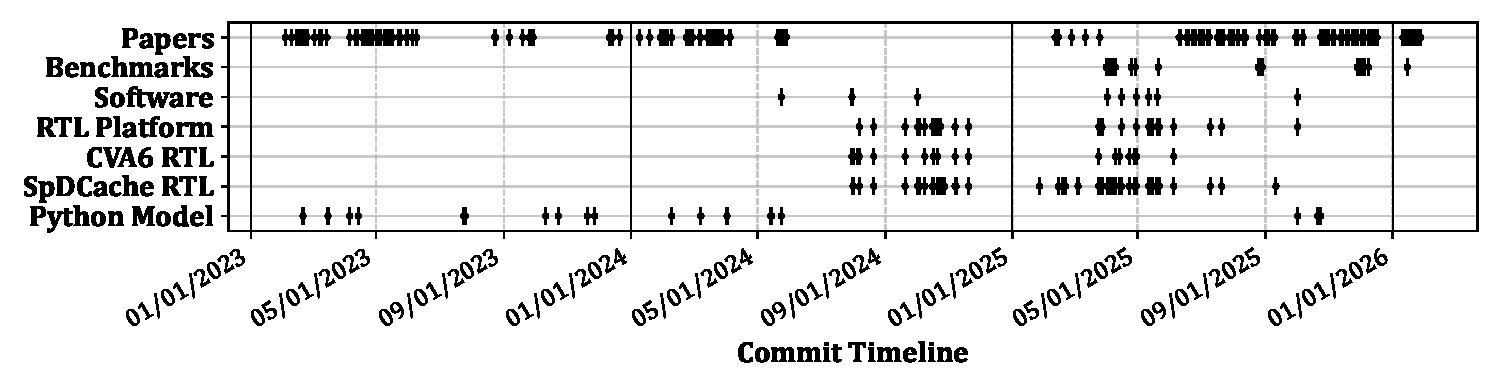
\includegraphics[width=\linewidth]{PreAndPostSections/Figures/PDF/Stats_Commits.pdf}
    \caption{Timeline of Commits Across All Working Repositories and Publications}
    \label{fig:app:stats:commits}
\end{figure}

To provide a sense of the work delivered, we present the number of new lines of code for each repository (excluding papers) after final modifications:
\begin{itemize}
    \item \textit{Python Scripts}: 18,590 lines;
    \item \textit{SpDCache RTL}: 5808 lines (33,696 $\to$ 39,504 total);
    \item \textit{CVA6 RTL}: 255 lines (36,623 $\to$ 36,878 total);
    \item \textit{RTL Platform}: 56 lines (6156 $\to$ 6212 total);
    \item \textit{Software}: 1554 lines;
    \item \textit{Benchmarks}: 7642 lines.
\end{itemize}
Additionally, Figure~\ref{fig:app:stats:languages} shows the programming language distribution across each repository.

\begin{figure}[htbp]
    \centering
    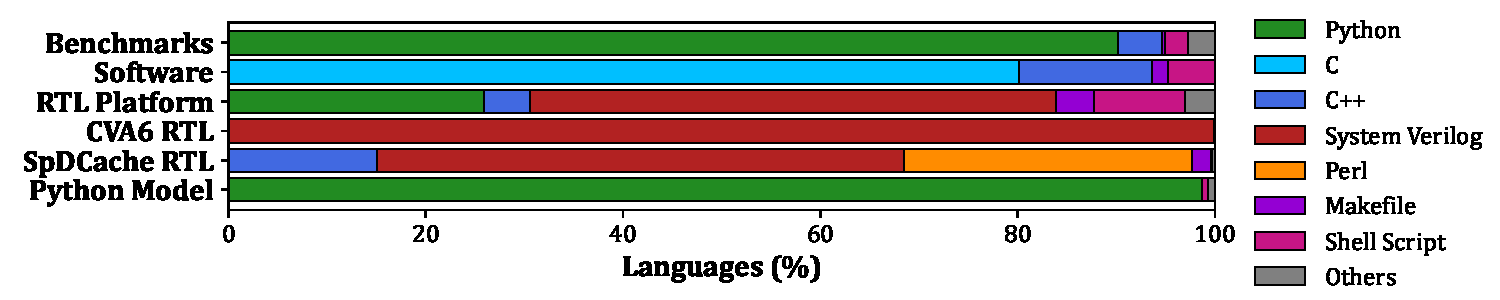
\includegraphics[width=\linewidth]{PreAndPostSections/Figures/PDF/Stats_Languages.pdf}
    \caption{Programming Language Distribution Across All Working Repositories}
    \label{fig:app:stats:languages}
\end{figure}

% %%%%%%%%%%%%%%%%%%%%%%%%%%%%%%%%%%%%%%%%%%%%%%%%%%%%%%%%%%%%%%%%%%%%%%%%%%%%%%%%%%%%%%%

\renewcommand{\thesection}{\arabic{chapter}.\arabic{section}}

\let\thefigure\originalthefigure
\renewcommand{\thefigure}{\thechapter.\arabic{figure}}

\let\thetable\originalthetable
\renewcommand{\thetable}{\thechapter.\arabic{table}}

\cleardoublepage %% Comment this line if this section occupies the last pages
\adjustmtc
% %%%%%%%%%%%%%%%%%%%%%%%%%%%%%%%%%%%%%%%%%%%%%%%%%%%%%%%%%%%%%%%%%%%%%%%%%%%%%%%%%%%%%%%
% List of Figures
% %%%%%%%%%%%%%%%%%%%%%%%%%%%%%%%%%%%%%%%%%%%%%%%%%%%%%%%%%%%%%%%%%%%%%%%%%%%%%%%%%%%%%%%

\FancyHeadRight{\sectitle}

\if\Language\EN \renewcommand{\sectitle}{List of Figures}
\else \renewcommand{\sectitle}{Table des figures} \fi

\phantomsection
\addcontentsline{toc}{chapter}{\sectitle}

\listoffigures

\cleardoublepage %% Comment this line if this section occupies the last pages
\adjustmtc
% %%%%%%%%%%%%%%%%%%%%%%%%%%%%%%%%%%%%%%%%%%%%%%%%%%%%%%%%%%%%%%%%%%%%%%%%%%%%%%%%%%%%%%%
% List of Tables
% %%%%%%%%%%%%%%%%%%%%%%%%%%%%%%%%%%%%%%%%%%%%%%%%%%%%%%%%%%%%%%%%%%%%%%%%%%%%%%%%%%%%%%%

\FancyHeadLeft{\sectitle}

\if\Language\EN \renewcommand{\sectitle}{List of Tables}
\else \renewcommand{\sectitle}{Liste des tableaux} \fi

\phantomsection
\addcontentsline{toc}{chapter}{\sectitle}

\listoftables

\cleardoublepage %% Comment this line if this section occupies the last pages
\adjustmtc
% %%%%%%%%%%%%%%%%%%%%%%%%%%%%%%%%%%%%%%%%%%%%%%%%%%%%%%%%%%%%%%%%%%%%%%%%%%%%%%%%%%%%%%%
% List of Algorithms
% %%%%%%%%%%%%%%%%%%%%%%%%%%%%%%%%%%%%%%%%%%%%%%%%%%%%%%%%%%%%%%%%%%%%%%%%%%%%%%%%%%%%%%%

\FancyHeadRight{\sectitle}

\if\Language\EN \renewcommand{\sectitle}{List of Algorithms}
\else \renewcommand{\sectitle}{Liste des algorithmes} \fi

\phantomsection
\addcontentsline{toc}{chapter}{\sectitle}
\renewcommand{\listalgorithmcfname}{\sectitle}

\listofalgorithms

\cleardoublepage %% Comment this line if this section occupies the last pages
\adjustmtc
% %%%%%%%%%%%%%%%%%%%%%%%%%%%%%%%%%%%%%%%%%%%%%%%%%%%%%%%%%%%%%%%%%%%%%%%%%%%%%%%%%%%%%%%
% List of Source Code
% %%%%%%%%%%%%%%%%%%%%%%%%%%%%%%%%%%%%%%%%%%%%%%%%%%%%%%%%%%%%%%%%%%%%%%%%%%%%%%%%%%%%%%%

\FancyHeadRight{\sectitle}

\if\Language\EN \renewcommand{\sectitle}{List of Source Code}
\else \renewcommand{\sectitle}{Table des codes sources} \fi

\phantomsection
\addcontentsline{toc}{chapter}{\sectitle}

\listofsourcecode

\cleardoublepage %% Comment this line if this section occupies the last pages
\adjustmtc
% %%%%%%%%%%%%%%%%%%%%%%%%%%%%%%%%%%%%%%%%%%%%%%%%%%%%%%%%%%%%%%%%%%%%%%%%%%%%%%%%%%%%%%%
%                             References
% %%%%%%%%%%%%%%%%%%%%%%%%%%%%%%%%%%%%%%%%%%%%%%%%%%%%%%%%%%%%%%%%%%%%%%%%%%%%%%%%%%%%%%%

\FancyHeadLeft{\sectitle}

\if\Language\EN \renewcommand{\sectitle}{Bibliography}
\else \renewcommand{\sectitle}{Bibliographie} \fi

\phantomsection
\addcontentsline{toc}{chapter}{\sectitle}

\bibliographystyle{ACM-Reference-Format}
\bibliography{biblio}

\cleardoublepage %% Comment this line if this section occupies the last pages
\adjustmtc
% %%%%%%%%%%%%%%%%%%%%%%%%%%%%%%%%%%%%%%%%%%%%%%%%%%%%%%%%%%%%%%%%%%%%%%%%%%%%%%%%%%%%%%%
%                             Table of content
% %%%%%%%%%%%%%%%%%%%%%%%%%%%%%%%%%%%%%%%%%%%%%%%%%%%%%%%%%%%%%%%%%%%%%%%%%%%%%%%%%%%%%%%

\FancyHeadRight{\sectitle}

\if\Language\EN \renewcommand{\sectitle}{Contents}
\else \renewcommand{\sectitle}{Table des matières} \fi

\phantomsection
\addcontentsline{toc}{chapter}{\sectitle}

\setcounter{tocdepth}{4}
\renewcommand{\contentsname}{\sectitle}
\tableofcontents

% \cleardoublepage %% Comment this line if this section occupies the last pages
\adjustmtc
% %%%%%%%%%%%%%%%%%%%%%%%%%%%%%%%%%%%%%%%%%%%%%%%%%%%%%%%%%%%%%%%%%%%%%%%%%%%%%%%%%%%%%%%

\end{document}